% THIS IS A LATEX TEMPLATE FILE FOR PAPERS INCLUDED IN THE
% *Anthology of Computers and the Humanities*. ADD THE OPTION
% 'final' WHEN CREATING THE FINAL VERSION OF THE PAPER. 
% DO NOT change the documentclass
%\documentclass[final]{anthology-ch} % for the final version
\documentclass[final]{anthology-ch}         % for the submission

% LOAD LaTeX PACKAGES
\usepackage{booktabs}
\usepackage{graphicx}
\usepackage{tabularx}
\usepackage{adjustbox}  % lets us make the table wider than \textwidth
\usepackage{setspace}
\usepackage{enumitem}
\usepackage{makecell}
% \usepackage{multirow}
\usepackage{float}
% \usepackage{url}
% \usepackage{cite}

% \usepackage[table,xcdraw]{xcolor} % Allows the use of HTML colors
% \usepackage{biblatex}
% \addbibresource{bibliography.bib}
\usepackage[numbers]{natbib}
\bibliographystyle{plainnat} % or choose another like IEEEtran, ACM-Reference-Format, etc.


% \PassOptionsToPackage{table,xcdraw}{xcolor}


\geometry{
  a4paper,
  top=2cm,
  bottom=2cm,
  left=2cm,
  right=2cm
}

% ADD your own packages using \usepackage{}

% TITLE OF THE SUBMISSION
% Change this to the name of your submission
\title{A Review of Reinforcement Learning Applications in Ad Policy Optimization for Large-Scale Recommender Systems}

% AUTHOR AND AFFILIATION INFORMATION
% For each author, include a new call to the \author command, with
% the numbers in brackets indicating the associated affiliations 
% (next section) and ORCID-ID for each author.  
\author{Armando Ordorica}

\author{Yuri Lawryshyn}

% While we encourage including ORCID-IDs for all authors, you can
% include authors that do not have one by definining an empty ID.


% There should be one call to \affiliation for each affiliation of
% the authors. Multiple affiliations can be given to each author
% and an affiliation can be given to multiple authors. 
\affiliation{University of Toronto, Toronto, Canada}

% KEYWORDS
% Provide one or more keywords or key phrases seperated by commas
% using the following command

\keywords{Reinforcement Learning, Ad Policy Optimization, Contextual Bandits, Recommendation Systems,  Off-Policy Learning, Online Advertising, Deep Reinforcement Learning,  Multi-Objective Optimization}

% METADATA FOR THE PUBLICATION
% This will be filled in when the document is published; the values can
% be kept as their defaults when the file is submitted
\pubyear{2025}
\pubvolume{1}
\pagestart{1}
\pageend{1}
\conferencename{Proceedings of Conference XXX}
\conferenceeditors{Editor1 Editor2}
\doi{00000/00000}  

% \addbibresource{bibliography.bib}


\setstretch{2.0}

\begin{document}


\maketitle
% \doublespacing

\begin{abstract}
Balancing advertisements with organic content in large-scale recommendation engines is a well-known challenge in the industry. While ads are essential for revenue generation in platforms that integrate them alongside organic content, they often underperform in user engagement compared to organic content \cite{hochstein2023toward}. The key challenges in achieving this balance include ad selection, ranking, and integration with organic content. These involve decisions about whether to insert an ad, which ad to select, and where to place it \cite{zhao2020jointly}. Traditional methods optimize for the highest probability of ad clickthrough with fixed placements and are typically solved as supervised Machine Learning (ML) problems \cite{covington2016deep}. However, these approaches focus on optimizing single actions, overlooking the downstream impact of sequential user behavior and underutilizing valuable contextual signals. A more dynamic approach that accounts for context and optimizes the long-term value of action sequences, balancing both engagement and revenue, remains an open research area \cite{lin2023survey}.\\

Reinforcement Learning (RL) offers a promising framework to address the need for dynamic, context-aware optimization by formalizing the process of finding the best policy in sequential decision-making under uncertainty \cite{dimitrakakis2018decision}. However, implementing RL in large-scale recommendation systems faces challenges such as vast state and action spaces, the risk of poorly chosen reward functions, high computational costs \cite{pancha2022pinnerformer}, and the difficulty of interpreting online policy learning \cite{van2024practical}. This paper surveys existing methodologies and frameworks that utilize RL to enhance recommendation strategies, aiming to guide practitioners and researchers in navigating these challenges. Our analysis reveals that while fully online RL is powerful in theory, in practice, techniques like contextual bandits, offline replay, and surrogate reward modeling often yield more scalable and interpretable solutions for large-scale ad-serving.
\end{abstract}

% \tableofcontents

\section{Introduction}

Platforms such as Google, Meta, TikTok, and Pinterest offer content recommendation systems whose revenue models depend on an effective balance between advertisements and organic content \cite{zhao2020jointly} \cite{danescu2010competing}. This balance is essential to maximize immediate revenue while avoiding long-term issues such as ad fatigue, where users become less responsive to ads due to overexposure, and user churn, where users discontinue using the platform \cite{sagtani2023quantifying} \cite{silberstein2023combating}.\\

Over the past decade, deep learning has emerged as a promising technique that enables recommendation engines to better understand context through embeddings, significantly improving their ability to personalize content \cite{naumov2019deep} \cite{zhao2024survey}. However, deep learning approaches are often supervised and rely on measurable and observable short-term metrics used as model labels, such as the probability of a click-through or the likelihood of a video being watched in full \cite{nvidia_recommender_systems_2021}. Methodologies that use myopic objective functions to optimize these directly measurable short-term metrics often overlook the long-term value of a recommendation \cite{mazoure2021improving}. By focusing on immediate rewards, they may rank content based on short-term engagement metrics while neglecting the entire sequence of user interactions that involve delayed responses. Such approaches can result in suboptimal outcomes, such as promoting clickbait content that compromises long-term revenue and user engagement.\\

	% 4.	How does Reinforcement Learning (RL) offer a promising solution to these challenges?

To overcome the challenges of optimizing based solely on immediate objectives, Reinforcement Learning (RL), modeled as a Markov Decision Process (MDP), has emerged as a promising framework \cite{afsar2022reinforcement}. RL enables the consideration of long-term value by optimizing policies that maximize cumulative rewards over time, rather than focusing on short-term engagement metrics. In an MDP, actions are selected based on a policy ($\pi$), which chooses the action that maximizes the expected cumulative reward from the current state onward. This cumulative reward is typically conceptualized as the expected sum of future rewards, discounted over time using a discount factor. A lower discount factor places more emphasis on immediate rewards, effectively ignoring future outcomes. Conversely, a discount factor approaching one values future rewards more heavily, encouraging the policy to consider long-term benefits \cite{Sutton1998}. \\

In the context of recommendation systems, rewards can be defined to capture both user engagement and revenue objectives. Engagement rewards might include metrics such as time spent on the platform, content views, clicks, saves, shares, or likes \cite{wang2022surrogate}. Revenue rewards can be tied to ad-related metrics like ad impressions, ad clicks, conversions, or purchases resulting from ad exposure. These different rewards are often combined into a single utility function that reflects the platform’s overall objectives \cite{zhao2020jointly} \cite{zou2019reinforcement} \cite{xu2023optimizing}.\\

For example, the reward function  $r_t$  at time  $t$  can be defined as:

$$
r_t = \alpha \times \text{Engagement Metric}_t + \beta \times \text{Revenue Metric}_t,
$$ where  $\alpha$  and  $\beta$  are weighting factors that balance the importance of user engagement and monetization. By appropriately defining the utility function and choosing suitable weights, RL algorithms can optimize policies that enhance user experience while maximizing revenue over the long term \cite{zhao2020jointly, zhao2021dear, yan2020ads, sagtani2024ad}. \\


% What specific challenges are encountered when implementing RL in large-scale recommendation systems?
Despite the promising theoretical framework that RL offers for optimizing long-term value in recommendation systems, implementing RL in real-world, large-scale platforms remains complex \cite{dulac2021challenges}. First, in the context of recommendation systems, the state space, which reflects the current context of the user and the environment, and the action space, which captures how the recommender system can be tuned, are both essentially infinite \cite{zhu2021overview}. This vastness makes learning and optimization computationally intensive and difficult to discretize into individual actions and states, a critical requirement for policy learning \cite{afsar2022reinforcement} . \\ 

Second, designing appropriate reward functions is critical, as poorly chosen reward functions can lead to unintended system behaviors that degrade user experience or negatively affect business revenue \cite{everitt2021reward}. For example, a reward function that overly prioritizes click-based metrics may drive the system to promote clickbait content, boosting short-term engagement but eroding user trust and satisfaction over time \cite{wu2017returning}. Similarly, a reward function too heavily skewed toward revenue metrics could result in excessive ad load, disrupting the user experience and leading to churn. Striking the right balance in reward function design is essential to achieve both user engagement and monetization objectives without compromising the platform’s long-term goals.\\


Furthermore, interpretability is a major challenge in RL deployment. Understanding the learned policies--the strategies adopted by the RL agent--can be particularly difficult when policies are updated in real-time during user interactions (online policy learning) \cite{glanois2024survey} \cite{vouros2022explainable} \cite{dulac2019challenges}. This real-time adaptation complicates monitoring and evaluation, making it challenging to understand what is happening during online learning. In extreme cases, this lack of transparency could result in non-compliant or unethical behavior, posing significant risks to both users and the business \cite{lambert2023entangled}.\\

	% 7.	What are the objectives and contributions of this paper?
In light of the challenges outlined above, this paper examines methodologies and frameworks used to implement RL for large-scale recommendation systems, with a particular focus on contexts where ad revenue is central to the business model. Although previous surveys address RL in recommendation systems \cite{lin2023survey, afsar2022reinforcement}, they do not specifically explore how RL can balance the competing demands of ad and organic content. This paper fills that gap by analyzing approaches tailored to these unique challenges and bridging the divide between theoretical RL concepts and their real-world applications.
\\

The paper begins with a historical overview of ad selection and ranking systems, tracing the evolution from simple rule-based models and heuristic approaches to tree-based models and modern deep learning techniques. Each of these stages is explored in detail, highlighting their limitations and the motivations for adopting RL as the next paradigm in recommendation systems. Following this contextual history and motivation, the paper introduces key RL components such as the action space, state space, reward functions, and policies, using a straightforward toy example: the frozen lake problem. This example provides a foundation for understanding RL fundamentals, which are then mapped to real-world challenges in online advertising and recommendation systems. Drawing on these analogies, the paper offers a clear and practical framework to help practitioners navigate the implementation of RL and adapt these methodologies to their specific needs.


	% 8.	How will this paper help practitioners and researchers navigate the challenges of implementing RL in recommendation systems?


	% 13.	What is the structure of the paper, and what can readers expect in the subsequent sections?

\section{Paper Collection Methodology}

To ensure broad coverage, relevant papers were collected from both academic and industry sources. Foundational academic works such as \textit{Reinforcement Learning: An Introduction} \cite{Sutton1998}, \textit{Statistical Methods for Recommender Systems} \cite{agarwal2016statistical}, and \textit{Artificial Intelligence: A Modern Approach} \cite{russell2016artificial} were used to establish key mathematical foundations, including Markov Decision Processes (MDPs), Contextual Bandits, Off-Policy Learning, and Offline Replay.

To reflect the internal perspective of a production-facing ad policy team, a curated list of 10–15 papers referenced within Pinterest’s Ad Policy team was also compiled. Examples include \textit{Jointly Learning to Recommend and Advertise} \cite{zhao2020jointly}, \textit{DEAR: Deep Reinforcement Learning for Online Advertising Impressions in Recommender Systems} \cite{zhao2021dear}, \textit{Ad-load Balancing via Off-Policy Learning} \cite{sagtani2024ad}, and \textit{Practical Bandits} \cite{van2024practical}. In addition, targeted keyword searches such as “Reinforcement Learning ads [company name]” and “Contextual Bandit [company name]” were conducted for leading companies in the advertising and recommendation space (e.g., Google, Meta, Pinterest, Microsoft, TikTok, YouTube, LinkedIn),  surfacing additional papers describing real-world systems and methodologies. To complement those efforts, a separate search was conducted on Google Scholar for relevant review papers. While no surveys were found that specifically focused on RL in ad recommendation systems, related reviews on "contextual bandits", "ad fatigue", and "recommender systems" were used to identify additional references.

Finally, manual crawling of citation networks in cornerstone papers was used to identify additional key contributions. For instance, tracing citations from \textit{Jointly Learning to Recommend and Advertise} \cite{zhao2020jointly}, \textit{DEAR} \cite{zhao2021dear}, and \textit{Offline Reinforcement Learning} \cite{levine2020offline} led to works such as \textit{Ads Allocation in Feed via Constrained Optimization} \cite{yan2020ads} and \textit{A Contextual Bandit Bake-off} \cite{bietti2021contextual}.
In total, 153 papers were selected and reviewed. Papers were ranked according to three main criteria: influence, to capture the foundational or widely adopted ideas in the field; industry relevance, to ensure that the outcomes were sound, implementable, and actionable; and recency, to reflect the latest methodological developments and deployment practices.

While recent and highly cited work was prioritized, papers introducing novel methodologies were also included regardless of citation count. To contextualize the selected works, this survey builds from the ground up. Each component of the Markov Decision Process, including states, actions, rewards, and policies, is defined and illustrated using a toy example such as the Frozen Lake. This foundation is then extended to practice through a review of how each component is operationalized in industry, along with a discussion of the limitations of those approaches. Drawing on existing methods and lessons from industry, the resulting framework is intended to inform practitioners exploring how RL can be applied in their organizations to develop ad policies that balance monetization with organic engagement. A comparison between the toy example and real-world implementation parallels can be found in Table \ref{tab:comparison}.



\section{A Brief History of Ad Selection and Ranking in Recommendation Systems}

\begin{figure}[ht]
    \centering
    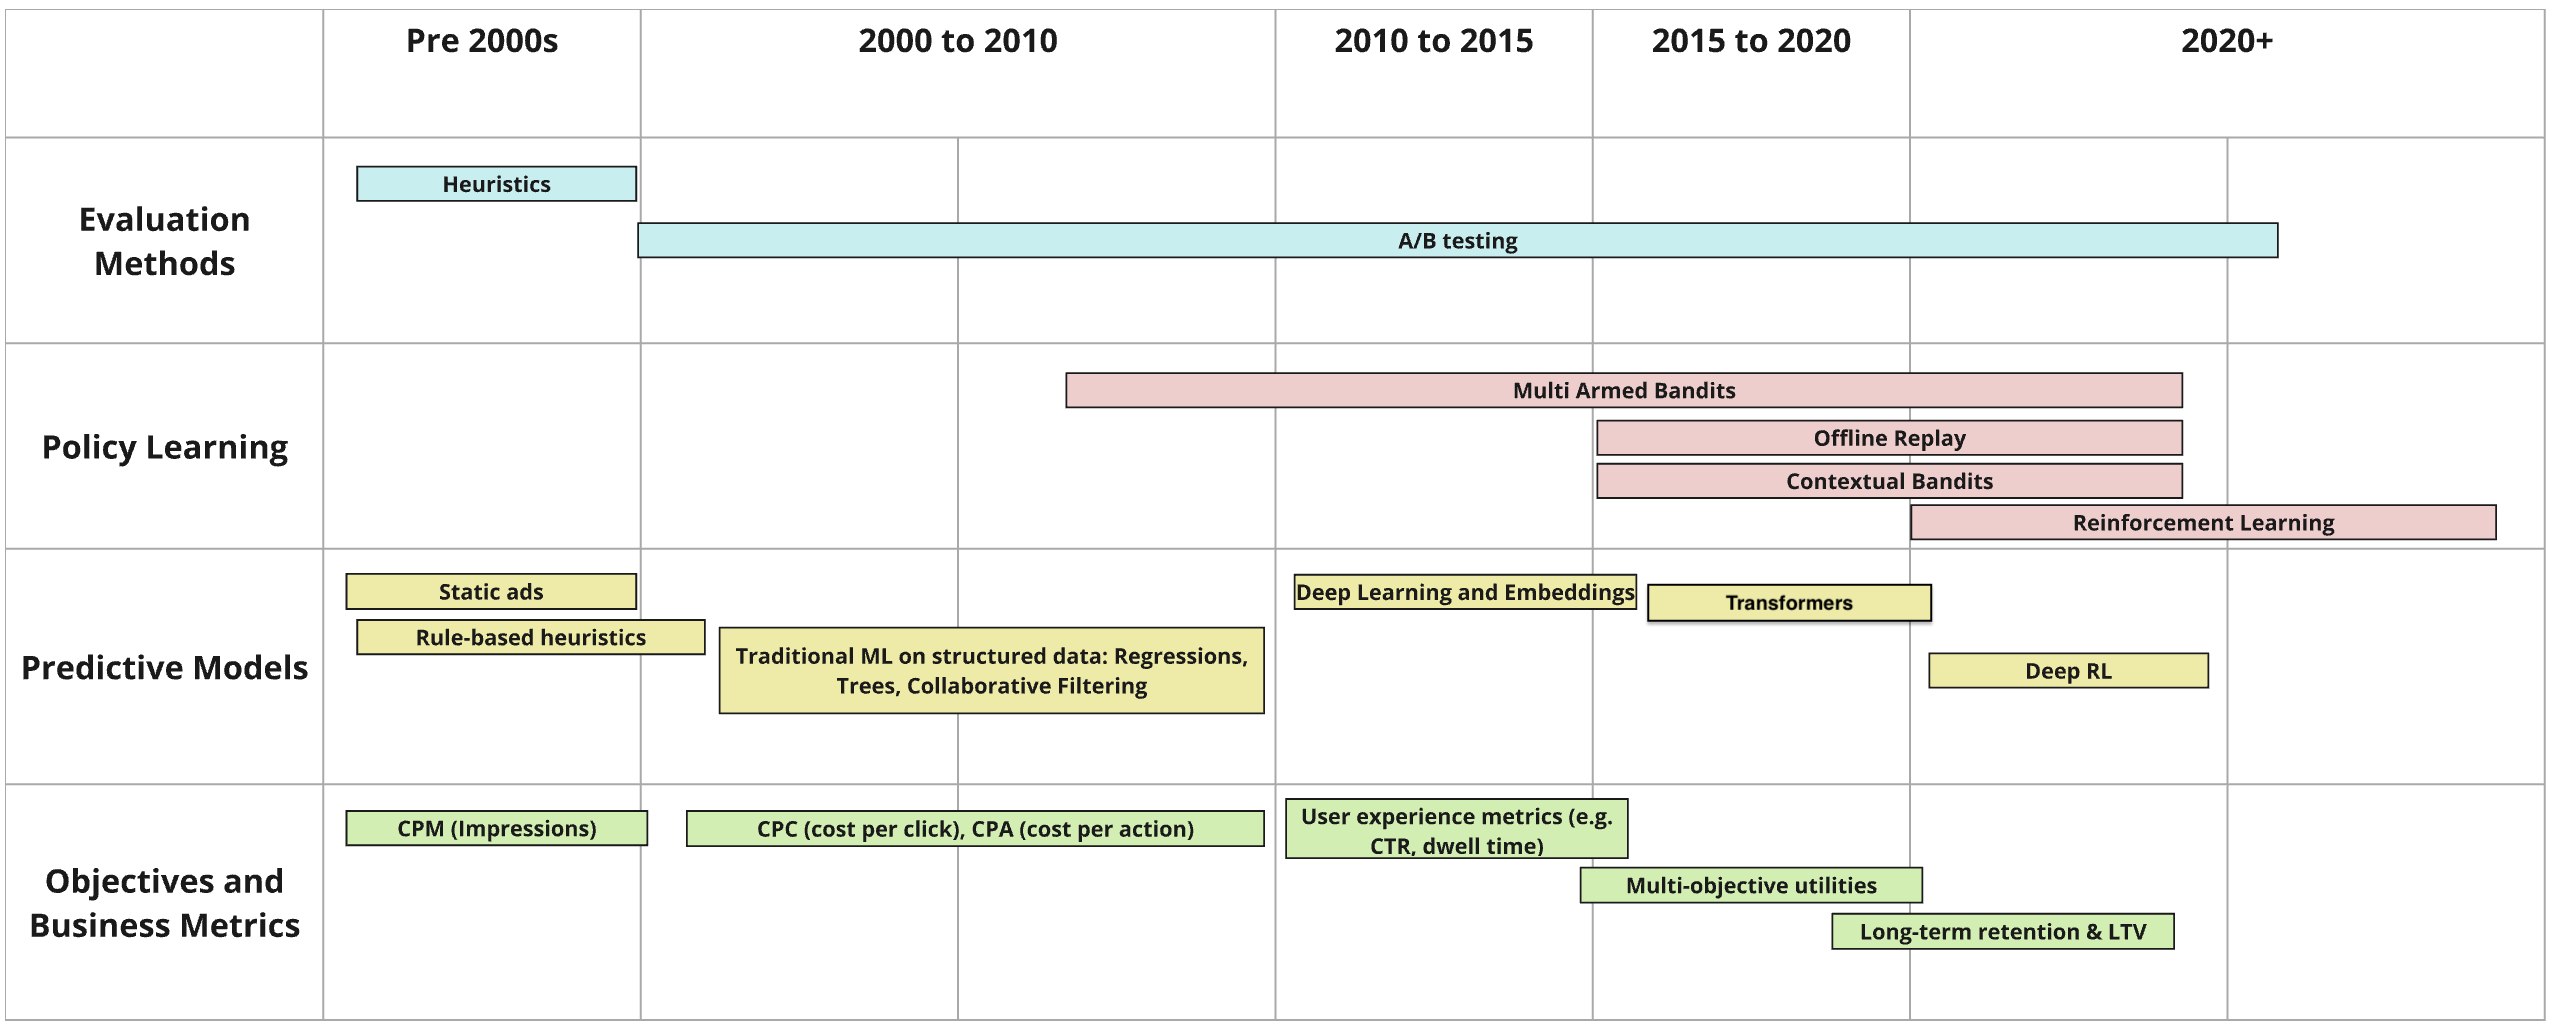
\includegraphics[width=\textwidth]{history_timeline_figure.png}
    \caption{Timeline Showing Initial Adoption and Popularization of Techniques and Methodologies in Online Advertising}
    \label{fig:ad_timeline}
    \vspace{0.2cm} % adds small vertical spacing
    \begin{flushleft}
        \footnotesize{\textit{Note:} The boundaries and lengths of rectangles are approximate. Innovations and transitions between techniques and objectives occurred gradually and continuously, rather than sharply at specific dates.}
    \end{flushleft}
\end{figure}


In online advertising, a good ad policy can result in positive revenue for the company while also boosting user experience. Conversely, a poor ad policy involves showing ads that are irrelevant to the user’s current intent, overloading the feed with excessive ad density, and failing to align content with the user’s interests. Irrelevant ad targeting can lead to ad fatigue, a state where users become desensitized or frustrated by excessive or poorly targeted ads, resulting in decreased engagement with both the ads and the platform as a whole \cite{ccelik2023ad}. \\

This section traces the evolution of advertising recommendation algorithms, culminating in the adoption of RL to overcome the limitations of earlier approaches. It begins by outlining how early online advertising primarily mirrored offline methods through banner ads and other static formats. It continues by explaining how static online advertising evolved over time to incorporate rule-based models and more sophisticated heuristic techniques. The discussion then transitions to the integration of machine learning methods, including regression-based models, tree-based algorithms, and collaborative filtering, followed by the emergence of deep learning and embedding-based approaches that effectively capture the nonlinear interactions between users and content. Finally, RL is introduced as a promising solution to address the shortcomings of preceding methodologies. This evolution is visually represented in Table \ref{fig:ad_timeline}, which shows the initial adoption and popularization of techniques and methodologies in online advertising. \\

\subsection{From Rule-Based Advertising to Traditional Machine Learning}
\textbf{Around the early 2000s, online advertising largely mirrored offline practices, heavily relying on non-targeted formats such as banner ads \cite{kant2021history}.} These generic advertising methods conflicted with the objective of search engines of efficiently directing users to relevant content \cite{fain2006sponsored}. As a marginal improvement on nontargeted ad formats like banner ads, advertisers began to utilize simple \texttt{if-then} logic with predefined rules to select and display ads based on basic criteria like user demographics. While rule-based systems were straightforward to implement, their lack of flexibility and personalization became evident as ad fatigue, defined as reduced user engagement due to repeated exposure to the same advertisement, persisted \cite{abrams2007personalized}. This issue underscored the necessity of not only leveraging user signals but also optimizing ad load tuning parameters, such as frequency and placement, to maintain user interest and maximize click-through rates \cite{abrams2007personalized}. For instance, researchers at LinkedIn introduced concepts like top slot - highest eligible position for an ad within the feed -  and minimum gap - the required distance between consecutive ads to prevent oversaturation - as ad load tuning parameters \cite{yan2020ads}. Their research indicated that users are more likely to click on ads that are spaced farther apart \cite{yan2020ads}. \\

\textbf{The evolution of ad pricing, from paying for impressions to paying for user actions, created pressure within the online advertising industry to improve relevance and performance-based metrics \cite{hu2004performance}.} Sponsored search, introduced by GoTo (later Overture), allowed advertisers to bid on specific keywords, directly linking ads to user queries and addressing the limitations of generic advertising  \cite{fain2006sponsored}. Foundational pricing models, such as Cost per Mille (CPM), charged advertisers per 1,000 impressions and closely mirrored offline practices \cite{wikipedia-cpm}. Yahoo!, through the acquisition of Overture \cite{wsj2003yahoooverture}, later introduced Cost per Click (CPC) \cite{ellam2003overture}, a performance-based pricing model that shifted costs to reflect measurable user engagement. This evolution continued with the introduction of Cost per Action (CPA), which tied fees to specific user actions beyond clicks, such as purchases or sign-ups. These changes incentivized the advertising industry to innovate, leading to the development of more relevance-focused strategies. These foundational pricing models remain integral to the utility functions that underpin contemporary ranking algorithms \cite{fain2006sponsored}. As advertisers increasingly demanded performance-based pricing, the ad tech industry was compelled to innovate within a competitive yet lucrative market, addressing the limitations of rule-based and heuristic models through the adoption of machine learning techniques to enable more dynamic and data-driven approaches \cite{zhang2018whole}.



\textbf{The next set of innovations following heuristics and performance-based targeting was led by machine learning (ML) and A/B testing \cite{barajas2022online}}. From 2010 to 2015, ad selection techniques evolved significantly with the adoption of machine learning models such as Logistic Regression, Decision Trees, and Gradient Boosting Machines \cite{cui2015global}. By leveraging historical data and diverse user behavior signals, these models enabled more accurate predictions of user engagement \cite{cui2015global}. In parallel, A/B testing allowed practitioners to systematically compare models and features, ensuring that any new implementation delivered measurable performance gains \cite{barajas2022online}.
Despite these successes, traditional tabular models struggled to capture nuanced user intent, particularly when processing more complex data such as images or text. In the early 2010s, deep learning gained momentum with breakthroughs like AlexNet \cite{krizhevsky2012imagenet}, which demonstrated the power of neural networks to handle unstructured high-dimensional data. This ability to capture complex, nonlinear interactions dramatically improved ad recommendations, especially through the use of embeddings, which are dense vector representations that map words or images into high-dimensional spaces. Metrics like cosine similarity further refined personalization by aligning recommendations with user interests \cite{covington2016deep}. Embedding-based models, particularly two-tower architectures, presented a major leap forward in ad recommendation systems by effectively capturing intricate relationships between users and ads. These models utilize two neural networks: one dedicated to encoding user information and the other to encoding ad (item) information. The outputs from these networks are then combined to predict user engagement with ads \cite{vorotilov2023scaling}. This approach not only boosted accuracy but also scaled effectively. Despite the significant improvements that embedding-based models introduced in terms of predictive accuracy and scalability of ad recommendation systems, the practical challenges of balancing multiple objectives, such as maximizing revenue, mitigating ad fatigue, and sustaining long-term user engagement remained unresolved.  


\textbf{Multi-Armed Bandits (MABs) emerged as a powerful method for online advertising around the 2010s to minimize user exposure to suboptimal ad configurations, effectively tackling the explore–exploit tradeoff, which consists of finding the optimal balance between choosing new ad policies with unknown performance and showing older ad policies with known positive performance \cite{schwartz2017customer} \cite{burtini2015improving}.} MABs are a class of algorithms for dynamic decision-making under uncertainty, originally developed in mid-20th-century probability theory \cite{robbins1952sequential}. While MABs had been widely applied in areas such as clinical trials \cite{villar2015multi} \cite{thompson1933likelihood}, they only gained significant traction in online advertising around the 2010s \cite{schwartz2017customer}.  

MABs allow platforms to reduce unnecessary exposure to a suboptimal treatment by continuously updating the probability distribution of which treatment is most likely to yield the highest reward \cite{kuleshov2014algorithms}. In clinical trials, for instance, a bandit algorithm reduces unnecessary exposure to suboptimal treatments by updating its reward estimates in real time: it allocates more patients to the better-performing treatment (exploitation) while still testing others that could be better (exploration) \cite{kuleshov2014algorithms}\cite{villar2015multi}. In this setting, the “reward” might be a measurable improvement in patient health or recovery time \cite{villar2015multi}. The same principle applies to online advertising, where “treatments” translate into specific ad configurations, defined by parameters such as displacement cost, reserve price, ad load, and ad placement. “Rewards” in online advertising typically represent user engagement metrics such as clicks or conversions \cite{schwartz2017customer}. Advertising platforms should continuously “explore” new treatments to test new ads, formats, and targeting strategies to avoid stagnation, while simultaneously “exploit” existing high-performing treatments to ensure near-term revenue targets are met \cite{schwartz2017customer}.  

In contrast to traditional A/B tests, where there are randomized treatments assigned for a predetermined amount of time, MABs dynamically learn which configuration yields the highest reward for each user at a particular time. This approach reduces the time users are exposed to suboptimal ad configurations, thereby mitigating losses in engagement and long-term revenue \cite{schwartz2017customer}. Although this dynamic learning framework effectively tackles the explore–exploit tradeoff, defining the precise set of rewards and objectives to optimize remains an open challenge, particularly when advertisers must juggle multiple goals such as revenue and long-term user satisfaction \cite{wen2019learning}.

\textbf{To address this need for clear, multi-objective definitions, such as balancing user satisfaction and revenue, utility functions have been employed in online advertising since the early 2000s \cite{engel2008incorporating}.} Rooted in microeconomic theory dating back to the mid-20th century, utility functions are mathematical constructs that quantify preferences and the net value of conflicting objectives \cite{Stigler1950} \cite{vonNeumannMorgenstern1944}. Introduced to formalize decision-making under uncertainty, they model and quantify consumer preferences, enabling advertisers and publishers to encode multiple objectives, such as revenue, user satisfaction, and long-term platform health, into a single or composite utility metric \cite{engel2008incorporating}. By integrating utility functions into MAB-based frameworks, advertisers can systematically guide the exploration–exploitation process toward a unified reward signal that balances short-term performance (e.g., clicks, impressions, or conversions) with long-term considerations (e.g., minimizing ad fatigue or maintaining user trust). This approach allows for principled trade-offs, optimizing for immediate gains while safeguarding long-term engagement.


\subsection{Advances in Deep Learning: Attention Models, Transformers, and Contextual Bandits}

\textbf{While embedding-based models greatly enhanced the predictive power of recommendation systems, capturing the full complexity of user sequences, especially over long time spans, remained a challenge for sequential deep learning methods such as  Long Short-Term Memory networks (LSTMs) and Gated Recurrent Units (GRUs) \cite{vaswani2017attention} \cite{gao2024mamba}.} Traditional recurrent networks (e.g., LSTMs or GRUs) process sequences step by step, typically encoding an entire sequence into a single fixed-size vector \cite{Sutskever2014}. This design poses several challenges. Because Recurrent Neural Networks (RNNs) operate strictly in a sequential manner, they cannot process multiple parts of the sequence in parallel, creating bottlenecks and risking the loss or blurring of details, especially those from earlier steps in long sequences \cite{vaswani2017attention}.  Moreover, standard RNNs inherently prioritize recent inputs as information is passed along, which attenuates earlier signals and leads to the well-known vanishing gradient problem in lengthy sequences and fails to effectively capture long-term dependencies \cite{Bengio1994}\cite{Pascanu2013}. 


\textbf{To address training inefficiencies in RNNs and the difficulty of capturing long-term dependencies, attention mechanisms allow direct access to any position in the sequence, enabling the model to focus on relevant features in the sequence regardless of their temporal distance \cite{vaswani2017attention}. }By computing pairwise interactions across all positions in the sequence, Transformers overcome the sequential bottlenecks of RNNs and enable parallel computation \cite{vaswani2017attention}.  This mechanism also allows the model to incorporate contextual signals, such as user demographics, session-level metadata, or item attributes, at any point in the sequence, rather than strictly depending on a running hidden state \cite{kang2018sasrec}. The ability to attend to any part of the input at any time allows Transformers to model long-range dependencies with far greater efficiency and accuracy than RNN-based architectures \cite{vaswani2017attention}. This paradigm shift led to the development of the Transformer architecture, which entirely replaces recurrence with self-attention, fundamentally redefining sequence modeling \cite{vaswani2017attention}.

\textbf{The Transformer’s parallel attention architecture is a natural fit for modern hardware.} Since self-attention and feed-forward layers are implemented with large matrix operations, the model makes efficient use of Graphics Processing Units (GPUs) and Tensor Processing Units (TPUs), which excel at parallel computation \cite{vaswani2017attention}. Unlike RNNs that left many GPU cores underutilized due to their step-by-step nature, Transformers keep the hardware busy by processing many elements concurrently. This yields significantly shorter training times compared to earlier recurrent models. Moreover, Transformers scale up seamlessly: training can be distributed across multiple GPUs, and larger batches or longer sequences can be handled without a drop in throughput \cite{shim2022comparison}. Engineers can simply add more GPU workers to accommodate bigger models or more data, achieving near-linear speedups in many cases \cite{brown2020language}. The ability to train deep models efficiently at scale has unlocked previously impractical projects, and Transformer-based architectures (e.g. BERT, GPT) are now standard building blocks in modern AI systems \cite{brown2020language} \cite{kaplan2020scaling}. One of the key innovations of the Transformer architecture is its multi-head attention mechanism \cite{vaswani2017attention}. Instead of relying on a single attention distribution, multiple attention “heads” are trained in parallel, each with its own set of learned parameters. This design allows the model to capture a range of relationships or patterns within the same sequence \cite{vaswani2017attention}.In practice, each head can focus on different aspects. One head might emphasize local dependencies in the user’s interaction history, while another one might highlight more global, long-range correlations \cite{vaswani2017attention}.


\textbf{In an advertising context, multi-head attention naturally accommodates multi-objective learning \cite{ma2018modeling}.} For example, one head could be tuned to prioritize short-term engagement metrics (e.g., click-through rate or CTR) by attending to recent user activities and relevant ad features, while another head could emphasize longer-term outcomes, such as mitigating ad fatigue or preserving user satisfaction \cite{zhao2019recommending} \cite{ma2018modeling}. Each head learns a distinct set of attention weights, enabling the model to isolate and capture unique signals that serve different goals \cite{an2024tmh}. The outputs from these multiple heads are then aggregated, typically concatenated and linearly transformed, into a single representation or score, providing a unified but multi-faceted embedding of user–ad interactions \cite{vaswani2017attention} \cite{lyu2023entire}. However, determining the appropriate attention heads and their optimal weighting remains a complex challenge \cite{vaswani2017attention}\cite{Kang2018} \cite{Voita2019}. The optimal weights may vary not only across different users and content types but also over time \cite{Zhou2018} \cite{Zhou2019}. Additionally, shifting business objectives, engineering constraints, and competing optimization objectives further complicate the design process \cite{Mehrotra2018} \cite{Mehrotra2020} \cite{Jannach2023}. 

%How is head selection and weighing typically done 
\textbf{Selecting the right heads in Multi-Task Attention Models and determining their optimal weighting is not a deterministic process \cite{Michel2019} \cite{Voita2019}.} It typically requires iterative experimentation, involving both offline analysis (e.g., hyperparameter tuning, head ablation studies) and online testing (A/B experiments) \cite{Michel2019} \cite{kang2018sasrec}. This process is particularly challenging for new users and new content, where slow adaptation can result in suboptimal personalization and early churn \cite{Schein2002, Bobadilla2013}. 

%tie this up to Offline Replay 
\textbf{To address difficulties related to policy optimization - like weight tuning and head selection - \textit{Offline Replay} is often employed to find optimal policies in large parameter search spaces  \cite{agarwal2016statistical} \cite{levine2020offline} \cite{agarwal2020optimistic}.} This technique typically begins with data collection via A/B/n experiments, where different policies are randomly assigned to users \cite{agarwal2019online} \cite{chen2009large}. Afterward, Offline Replay simulates the effects of various ad policies across different user segments and estimates the potential rewards based on logged interactions \cite{agarwal2016statistical}. In this context, “reward” refers to the performance metric we aim to maximize (i.e. clicks, likes, shares, revenue) \cite{wu2017returning}. However, in many cases, the true optimal treatment is not explicitly tested \cite{agarwal2019online}. Here, importance sampling corrects for differences between the observed behavior policy and the target policy, improving estimation accuracy \cite{Sutton1998} \cite{dudik2011doubly}.  Based on the collected data on random assignments between policies and users typically involved in Offline Replay, one can use different policy learning methods to map the optimal policies from user ids, content types, and other contextual signals for the optimal weights at any point in time \cite{swaminathan2015counterfactual}. 


%  As a form of counterfactual learning, it estimates potential rewards under different policies by simulating outcomes based on logged interactions. This enables the system to learn from sparse or delayed feedback and serves as a critical tool for safely testing new policies offline \cite{sagtani2024ad}.\\

% In this context, “reward” refers to the performance metric we aim to maximize. For example, a click or any other positive action on an item is considered a reward. Sometimes, a positive action like a click can be weighted by a downstream utility, such as advertising revenue or time spent on a landing page (the page displayed after a user clicks on a recommended item), to derive a weighted reward. Our goal is to estimate the expected reward of a new ad policy using data collected in the past \cite{agarwal2016statistical}.\\

\textbf{Offline replay  often assumes that user preferences and item availability do not change significantly during data collection. }However, in real ad systems, these factors can shift, causing offline data to become stale or biased \cite{levine2020offline} \cite{agarwal2014taming}. Contextual bandits address this limitation by leveraging continuous feedback from live user interactions, preventing the policy from being locked into a static offline dataset \cite{li2010contextual}. Contextual bandits can be thought of as a special case of RL, where an action selection does not influence future states \cite{bubeck2012regret} \cite{Sutton1998}. Unlike full RL, which models long-term state transitions, contextual bandits assume that each decision is independent, optimizing for immediate rewards rather than a multi-step trajectory \cite{bubeck2012regret} \cite{Sutton1998}. This makes them particularly well-suited for recommender systems, where ranking decisions can be treated as independent events \cite{afsar2022reinforcement} \cite{zhou2016latent}. Additionally, contextual bandits naturally balance exploration and exploitation, allowing them to adapt dynamically to user behavior in real time \cite{li2010contextual}. However, a practical limitation of contextual bandits is that they select actions from a fixed set defined at deployment time, such as preconfigured ad policies or treatment arms \cite{bietti2021contextual}. As a result, the policy’s performance is inherently constrained by the quality and granularity of the available states and actions at the time of inference \cite{dimitrakakis2018decision}.

\textbf{Although contextual bandits inherently focus on short-term rewards, they can be tuned to approximate long-term objectives by encoding historical or delayed outcomes into the feature space or the immediate reward function \cite{mcdonald2023impatient} \cite{wu2017returning}.} For instance, if an attention head emphasizing ad engagement indirectly correlates with better retention, a contextual bandit can increase its weight over time, provided that retention signals are reflected in the contextual features or the reward proxy \cite{yi2023progressive}. However, full RL remains more appropriate for scenarios demanding explicit multi-step optimization, where actions taken now significantly shape future user states \cite{gauci2018horizon}. Contextual bandits thus offer a practical trade-off, providing continuous adaptation and efficient online learning without the computational complexity of fully modeling multi-step state transitions \cite{gauci2018horizon} \cite{levine2020offline}.


\textbf{Despite the practical advantages that contextual bandits offer for real-time experimentation and short-horizon reward maximization, they remain limited in scenarios where user states evolve over repeated interactions \cite{Sutton1998}.} Modern advertising platforms often contend with extended user sessions and multiple recurring visits, demanding an approach capable of modeling multi-step feedback loops. RL naturally extends these capabilities by incorporating stateful dynamics and cumulative rewards, capturing phenomena like ad fatigue \cite{ccelik2023ad} and long-term retention \cite{wu2017returning}. Recent industrial deployments underscore RL’s growing importance in ads: ByteDance uses RL-based systems \cite{zhao2020jointly,zhao2021dear} to balance immediate revenue with session-level engagement in short-video feeds, Meta (Facebook) has leveraged policy-gradient methods for sequencing notifications and ad placements over evolving user states \cite{gauci2018horizon}, and companies like Google are experimenting with RL-driven ad scheduling that accounts for shifting user contexts at scale \cite{zhao2024survey}. These efforts demonstrate how RL can transcend the myopic focus of bandits to address long-horizon outcomes, multi-objective trade-offs, and dynamic user behaviors. In the sections that follow, we explore how these RL paradigms are integrated into large-scale advertising stacks, focusing on core algorithms, design decisions, and lessons learned from real-world implementations.



\section{The RL formulation of the Ad Recommendation Problem}

In RL, the \textbf{GridWorld problem }is a foundational example of a Markov Decision Process (MDP), where an \textbf{agent} interacts with a \textbf{deterministic environment} by performing \textbf{discrete actions}, such as moving up, down, left, or right, to navigate through a grid with the objective of reaching a goal, while potentially avoiding obstacles or hazards. A more complex variant is the \textbf{FrozenLake problem}, which features a \textbf{stochastic environment} where movements are uncertain due to a slippery surface (\textcolor[HTML]{1E90FF}{F}) as shown in Figure~\ref{tab:frozen_lake} \cite{FrozenLakeGymnasium2023}. Here, \textbf{actions do not always lead to the intended next state}, adding complexity by requiring policies that effectively manage uncertainty. In this paper, \textbf{we use the FrozenLake problem as a representative framework for stochastic environments and leverage this template to describe the ad optimization problem as an RL task}. Specifically, we will explore components of the underlying MDP, such as states, actions, and rewards, and investigate key RL concepts including policy evaluation, value iteration, and policy iteration. The grid is typically represented as shown in Figure~\ref{tab:frozen_lake}:


\label{frozen_lake}


\begin{figure}[ht]
\centering
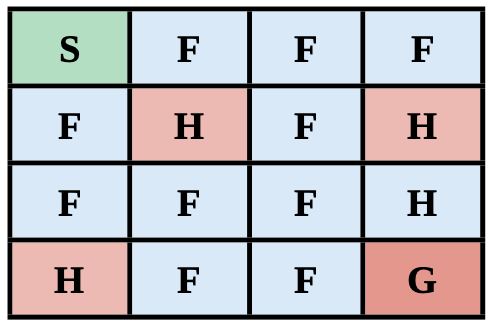
\includegraphics[width=0.35\linewidth]{frozenlake-table.png}
\caption{Frozen Lake Environment Grid}
\label{tab:frozen_lake}
\end{figure}


% \begin{table}[ht]
%     \centering
%     \setlength{\arrayrulewidth}{0.5mm}
%     \setlength{\tabcolsep}{12pt}
%     \renewcommand{\arraystretch}{1.5}
%     \begin{tabular}{|c|c|c|c|}
%         \hline
%         \cellcolor[HTML]{A9DFBF}\textbf{S} & \cellcolor[HTML]{D6EAF8}\textbf{F} & \cellcolor[HTML]{D6EAF8}\textbf{F} & \cellcolor[HTML]{D6EAF8}\textbf{F} \\ \hline
%         \cellcolor[HTML]{D6EAF8}\textbf{F} & \cellcolor[HTML]{F5B7B1}\textbf{H} & \cellcolor[HTML]{D6EAF8}\textbf{F} & \cellcolor[HTML]{F5B7B1}\textbf{H} \\ \hline
%         \cellcolor[HTML]{D6EAF8}\textbf{F} & \cellcolor[HTML]{D6EAF8}\textbf{F} & \cellcolor[HTML]{D6EAF8}\textbf{F} & \cellcolor[HTML]{D6EAF8}\textbf{H} \\ \hline
%         \cellcolor[HTML]{F5B7B1}\textbf{H} & \cellcolor[HTML]{D6EAF8}\textbf{F} & \cellcolor[HTML]{D6EAF8}\textbf{F} & \cellcolor[HTML]{F1948A}\textbf{G} \\ \hline
%     \end{tabular}
%     \caption{Frozen Lake Environment Grid}
%     \label{tab:frozen_lake} % This label is used to reference the table
% \end{table}


\begin{table*}[ht]
    \centering
    \small
    \begin{tabular}{|>{\centering\arraybackslash}p{3cm}|p{3.5cm}|p{9cm}|}
        \hline
        \textbf{Component of Markov Decision Process Formulation} & \textbf{Frozen Lake Example} & \textbf{Large Scale Recommendation Systems for Ad Policy Optimization} \\ 
        \hline
        \textbf{Environment} & The frozen lake. & The users. \\ 
        \hline
        \textbf{Goal} & Reach the goal (G) from the start position (S) while avoiding holes (H). The agent must avoid falling into a hole, and reaching the goal faster is rewarded. & Maximize revenue without compromising user experience. \\ 
         \hline
          \textbf{Episode} & A game. & A time period (T), typically 2 weeks, corresponding to an A/B experiment where enough data is collected to evaluate policy performance across users. \\ 
        \hline
        \textbf{Rewards} & Rewarded for reaching the goal (i.e., +100), but penalized for delays (i.e., -1 per step). & 
        The reward is typically represented by a utility function, which could be a weighted sum of metrics like user engagement (clicks, time spent) and revenue generated (ad clicks, conversions). The challenge lies in balancing short-term revenue with long-term user retention. \\ 
        \hline
        \textbf{Agent} & The learner. & The Recommendation System. \\ 
        \hline
        \textbf{Actions} & Up, down, left and right. & 
        Basically infinite. But when it comes to ad recommendations specifically, some typical actions are the following: 
        \begin{itemize}
            \item Reserve Price Floor: The minimum price at which an ad impression is sold.
            \item Displacement Cost Threshold: A measure of the opportunity cost for showing an ad.
            \item Max Ad Load: The maximum number of ads that can be shown without reducing user satisfaction.
            \item Ad Quality Thresholds: Standards used to ensure ads meet a quality bar before being shown.
            \item Ad Placement: The specific position of ads within the user feed (e.g., first, third, or fifth position).
        \end{itemize} \\
        \hline
        \textbf{States} & All possible grid positions the agent can occupy, representing the state space of the environment. & 
        \textbf{Signals}:
        \begin{itemize}
            \item User Context: Demographics, user profile
            \item Interaction Data: Previous interactions with ads, organic content
            \item Contextual Features: Time of day, browsing context
            \item Embeddings: Latent feature representations of user interests or ad features
        \end{itemize} \\
        \hline
        \textbf{Policy} & A mapping of grid positions to optimal action to take for a maximum reward. & 
        A mapping of user segments to ad treatments to maximize both revenue and user experience. This policy can be dynamically adjusted based on real-time feedback or offline simulations. \\ 
        \hline
    \end{tabular}
    \caption{Comparison of Frozen Lake Example and Large-Scale Recommendation Systems for Ad Policy Optimization}
    \label{tab:comparison}
\end{table*}

\subsection{The Agent and its Objective}
While toy examples like GridWorld \cite{Sutton1998}  and Frozen Lake \cite{frozenlake} provide well-defined, relatively simple environments where RL algorithms can be easily tested, transitioning these insights to real-world recommendation systems is far more complex due to factors like vast state–action spaces and delayed rewards, and environment observability \cite{dulac2019challenges, kaelbling1996reinforcement}. \textbf{Observability refers to the degree to which an agent can directly perceive the complete state of the environment} \cite{kaelbling1998planning}. In fully observable settings (such as the FrozenLake), the agent sees the true state at every step, enabling straightforward decision-making \cite{kaelbling1998planning}. However, real-world environments, including \textbf{recommendation systems, are often partially observable \cite{lu2016partially}}; the agent must infer the underlying state from incomplete or noisy signals, increasing both the computational complexity of learning and the uncertainty of policy outcomes \cite{wu2021partially}. In the FrozenLake environment, the \textbf{agent is a decision-maker that observes its surroundings and chooses actions}. It learns to navigate the grid to reach the goal (\textcolor[HTML]{FF4500}{G}) from the start position (\textcolor[HTML]{228B22}{S}) while avoiding holes (\textcolor[HTML]{FF0000}{H}) and navigating slippery surfaces (\textcolor[HTML]{1E90FF}{F}). By analogy, in ad policy optimization, \textbf{the agent is the algorithm responsible for serving ads}, which must balance two primary \textbf{objectives}: maximizing revenue while maintaining (or ideally enhancing) user engagement \cite{Theocharous-2015, zou2019reinforcement}. Ultimately, both the FrozenLake agent and the ad-serving algorithm share the same high-level goal: to maximize long-term rewards through strategic actions grounded in observed states.

The use of a \textbf{reward signal} to formalize the idea of a goal is a distinctive feature of RL \cite{Sutton1998}. In an MDP, the reward is a scalar value the agent receives after taking an action in a given state and transitioning to a new state, serving as immediate feedback on the benefit or cost of the action \cite{kaelbling1996reinforcement}. This feedback allows the agent to learn a policy that maximizes the cumulative reward over time \cite{kaelbling1996reinforcement}. In simple RL scenarios, rewards are typically straightforward. For instance, the agent might receive -1 per move (to encourage shorter paths), +100 for reaching the goal (G), and -100 if it falls into a hole (H), ending the episode. \textbf{However, in real-world recommendation systems, reward structures can be far more nuanced.  It is often unclear which user behaviors warrant the highest reward or how to weigh different signals} \cite{mcdonald2023spotify}. In online advertising, for example, low-intent actions such as clicks may be valued less than high-intent actions like saves or purchases. Moreover, deciding how to balance these varied signals in a single reward function can be both subjective and complex, especially when multiple objectives (e.g., revenue, user satisfaction, and content diversity) must be optimized \cite{mcdonald2023spotify}.\\

Ad recommendation engines often need to \textbf{balance multiple objectives}, such as maximizing user engagement while also ensuring ad revenue \cite{zhang2018whole, yan2020ads, sagtani2024ad}. Long-term engagement and revenue are metrics that are particularly difficult to measure directly, especially in randomized controlled experiments that typically span only a couple of weeks \cite{mcdonald2023spotify}. The delay in outcomes (e.g., retention signals may take months to manifest) and the often subtle impact of a single intervention can make it nearly impossible to detect meaningful changes within such short time frames \cite{mcdonald2023spotify}.  As a result, proxy metrics are commonly used. For instance, click-through rate (CTR) and ad impressions serve as approximate measures of revenue, while session duration, saves, and shares act as proxies for longer-term engagement \cite{wang2022surrogate}. However, these simpler proxies can fail to capture the system’s true long-term objectives, occasionally leading to suboptimal policies \cite{mazoure2021improving}. A high CTR may reflect short-term engagement, yet it can ultimately induce ad fatigue or frustrate users if the ads are misaligned with their actual interests \cite{hohnhold2015focusing, sagtani2024ad}. Table \ref{fig:proxy-metrics} summarizes some of the most commonly used proxies in the industry across dimensions of revenue, engagement, and ad fatigue. 


% \begin{figure}[H]
% \centering
% 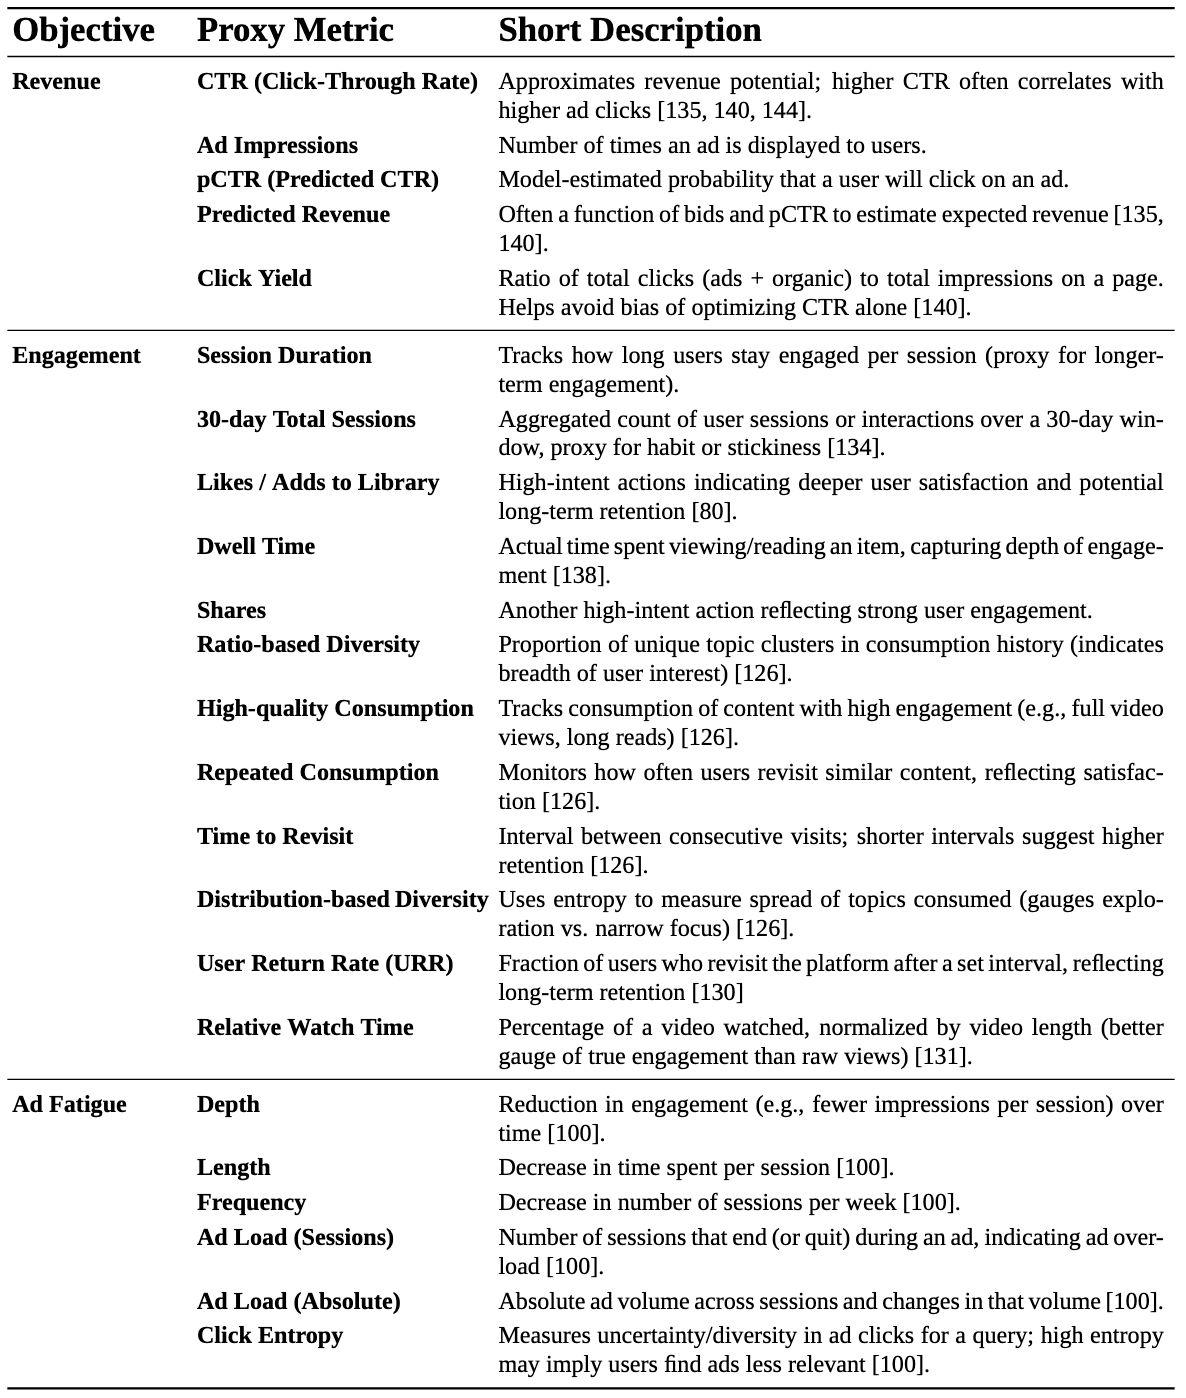
\includegraphics[width=\linewidth]{proxy-metrics-table.png}
% \caption{Proxy metrics for Revenue, Engagement, and Ad Fatigue.}
% \label{fig:proxy-metrics}
% \end{figure}

\begin{figure}[ht]
  \centering
  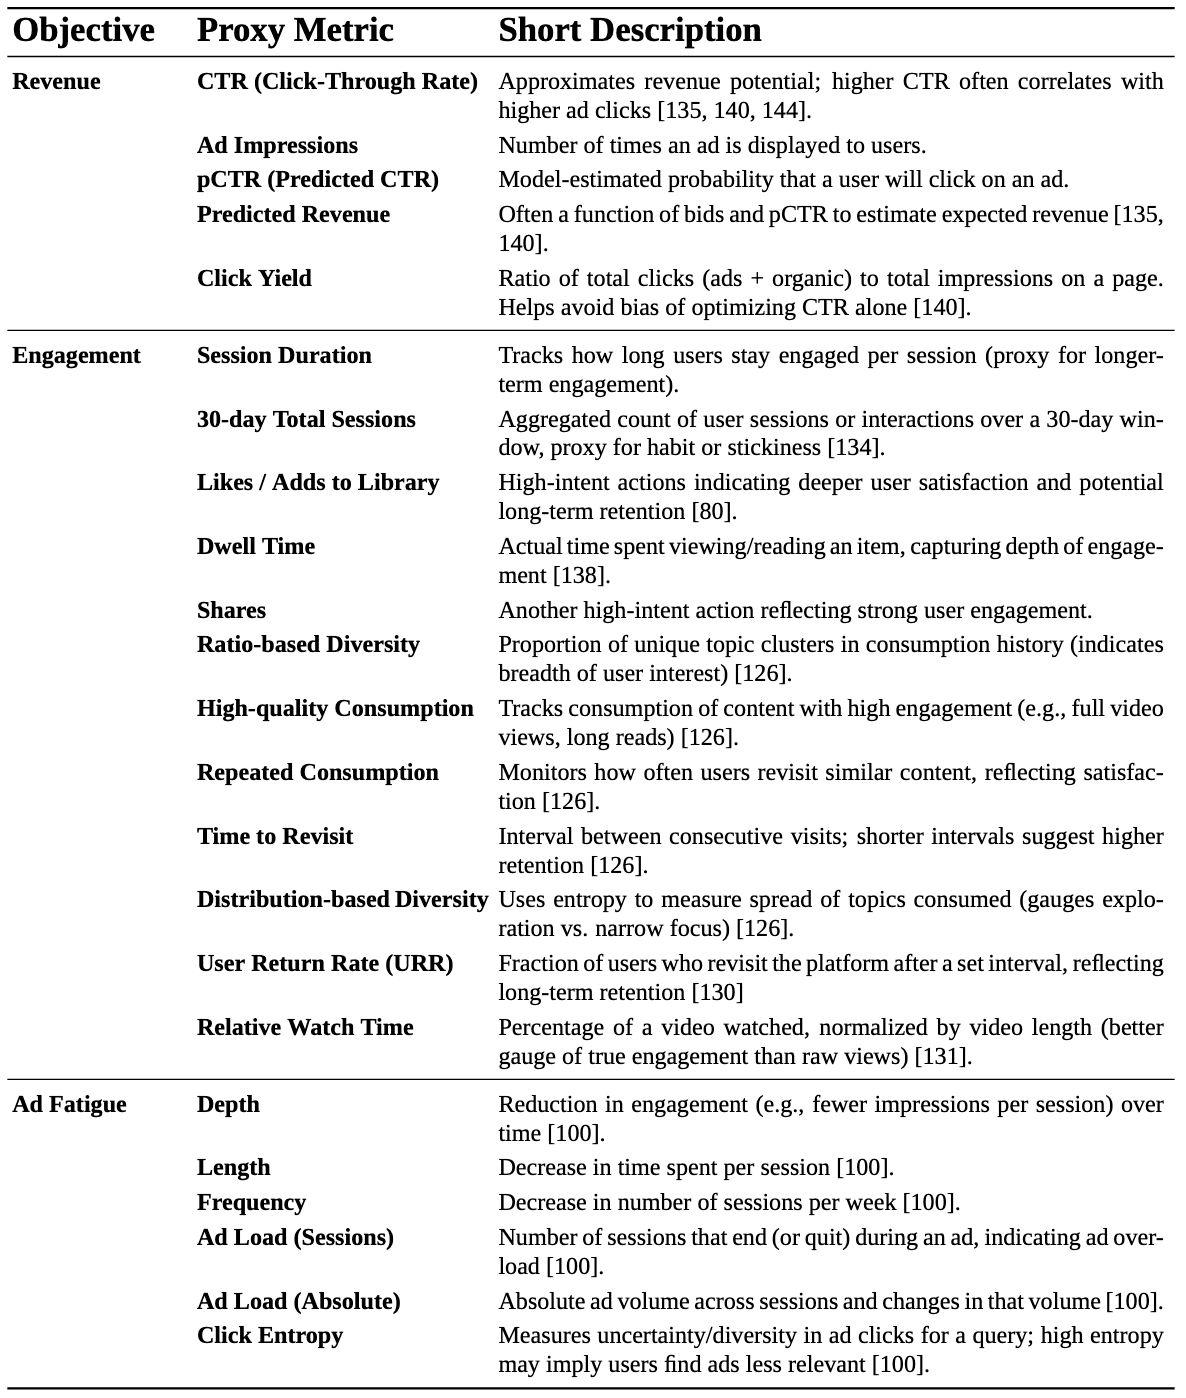
\includegraphics[width=\textwidth, height=0.85\textheight, keepaspectratio]{proxy-metrics-table.png}
  \caption{Proxy metrics for Revenue, Engagement, and Ad Fatigue.}
  \label{fig:proxy-metrics}
\end{figure}


% \begin{table}[H]
% \setstretch{1} % Ensure normal spacing within table. Separation between lines of the same cell. 
% \centering
% \small
% \renewcommand{\arraystretch}{1.2}  % Tweak if needed
% \setlength{\tabcolsep}{2pt} % separation between columns 
% \begin{tabularx}{\linewidth}{p{0.15\linewidth} p{0.25\linewidth} p{0.57\linewidth}}
% % the decimal points allow to control the size of the table, not of the text.
% \toprule
% {\bfseries \Large Objective} & {\bfseries \Large Proxy Metric} & {\bfseries \Large Short Description} \\
%   % \textbf{Objective} & \textbf{Proxy Metric} & \textbf{Short Description} \\
% \midrule
%     \multirow{\textbf{Revenue}} 
%        & \textbf{CTR (Click-Through Rate)} 
%            &  Approximates revenue potential; higher CTR often correlates with higher ad clicks \cite{zhang2018whole, yan2020ads, zhao2020jointly}. \\
%        & \textbf{Ad Impressions} 
%            & Number of times an ad is displayed to users. \\
%        & \textbf{pCTR (Predicted CTR)} 
%            & Model-estimated probability that a user will click on an ad. \\
%        & \textbf{Predicted Revenue} 
%            & Often a function of bids and pCTR to estimate expected revenue  \cite{yan2020ads, zhang2018whole}. \\
%        & \textbf{Click Yield} 
%            & Ratio of total clicks (ads + organic) to total impressions on a page. Helps avoid bias of optimizing CTR alone \cite{zhang2018whole}. \\
%     \midrule
%     \multirow{\textbf{Engagement}} 
%        & \textbf{Session Duration} 
%            & Tracks how long users stay engaged per session (proxy for longer-term engagement). \\
%         & \textbf{30-day Total Sessions} 
%        & Aggregated count of user sessions or interactions over a 30-day window, proxy for habit or stickiness 
%        \cite{xu2023optimizing}. \\
%        & \textbf{Likes / Adds to Library} 
%        & High-intent actions indicating deeper user satisfaction and potential long-term retention \cite{mcdonald2023spotify}. \\
%           & \textbf{Dwell Time} 
%        & Actual time spent viewing/reading an item, capturing depth of engagement  \cite{yi2014beyond}. \\
%        & \textbf{Shares} 
%            & Another high-intent action reflecting strong user engagement. \\
%     & \textbf{Ratio-based Diversity}  
%            & Proportion of unique topic clusters in consumption history (indicates breadth of user interest) \cite{wang2022surrogate}. \\
%        & \textbf{High-quality Consumption} 
%            & Tracks consumption of content with high engagement (e.g., full video views, long reads) \cite{wang2022surrogate}. \\
%      & \textbf{Repeated Consumption}  
%            & Monitors how often users revisit similar content, reflecting satisfaction \cite{wang2022surrogate}. \\
%               & \textbf{Time to Revisit} 
%            & Interval between consecutive visits; shorter intervals suggest higher retention \cite{wang2022surrogate}. \\
%      & \textbf{Distribution-based Diversity}  
%            & Uses entropy to measure spread of topics consumed (gauges exploration vs. narrow focus) \cite{wang2022surrogate}. \\
%     & \textbf{User Return Rate (URR)} 
%        & Fraction of users who revisit the platform after a set interval, reflecting long-term retention  \cite{wu2017returning} \\
%      & \textbf{Relative Watch Time} 
%        & Percentage of a video watched, normalized by video length (better gauge of true engagement than raw views) 
%       \cite{wu2018beyond}. \\
%     \midrule
%     \multirow{\textbf{Ad Fatigue}} 
%        & \textbf{Depth} 
%            & Reduction in engagement (e.g., fewer impressions per session) over time \cite{sagtani2023quantifying}. \\
%        & \textbf{Length} 
%            & Decrease in time spent per session \cite{sagtani2023quantifying}. \\
%        & \textbf{Frequency} 
%            & Decrease in number of sessions per week \cite{sagtani2023quantifying}. \\
%        & \textbf{Ad Load (Sessions)} 
%            & Number of sessions that end (or quit) during an ad, indicating ad overload \cite{sagtani2023quantifying}. \\
%        & \textbf{Ad Load (Absolute)} 
%            & Absolute ad volume across sessions and changes in that volume \cite{sagtani2023quantifying}. \\
%        & \textbf{Click Entropy} 
%            & Measures uncertainty/diversity in ad clicks for a query; high entropy may imply users find ads less relevant \cite{sagtani2023quantifying}. \\
% \bottomrule
% \end{tabularx}
% \caption{Proxy metrics for Revenue, Engagement, and Ad Fatigue.}
% \label{tab:proxy-metrics}
% \end{table}




\textbf{Utility functions are mathematical constructs used to estimate the net value of conflicting objectives \cite{Stigler1950}.} A utility function is a \textbf{composite reward function} that allows the agent to integrate various rewards or metrics from multiple objectives using a unified currency, facilitating more nuanced decision-making across competing priorities \cite{Stigler1950}. The ability to compare two utilities, like those of revenue and engagement normalized to a common scale, is critical for any principled blending of organic items and ads \cite{yan2020ads}.  Most utility functions are linear though this linearity is not a requirement for how the individual utility of each component is calculated \cite{wen2019learning, zhao2020jointly}. 

A \textbf{canonical utility function} at the policy layer to \textit{blend} ads and organic content can be represented as follows \cite{sagtani2024ad, yan2020ads, carrion2021blending}:
    \begin{equation}
        U(x) = \alpha \times \text{Revenue} + \beta \times \text{Engagement} - \gamma \times \text{Ad Fatigue}
    \end{equation}
    where $\alpha$, $\beta$, and $\gamma$ are weights that determine the relative importance of each factor. To compute the utilities of "Revenue", "Engagement", and "Ad Fatigue", typically many signals feed into each component. These signals include, but are not limited to, the ones shown in Table \ref{fig:proxy-metrics}. In a bandit or RL context, $U(x)$ serves as the reward signal guiding policy updates. The process of tuning the weights of $\alpha$, $\beta$, and $\gamma$ is often done through experimentation, as the right balance between engagement and revenue can shift depending on the context. For instance, ByteDance uses a multi-objective reward framework in their recommendation systems, where different reward functions are designed for organic content and ads, combining them to guide the overall recommendation strategy \cite{zhao2020jointly}.
    
In some cases, a very simple unified function can suffice over a complex utility function. Researchers at Alibaba introduced the concept of Click Yield, which is defined as the ratio of the total number of clicks on all items (ads + organic results) to the total number of impressions on a page \cite{zhang2018whole}. Click Yield provides a holistic evaluation of page performance, accounting for the interactive effects between ads and organic content, and helping to mitigate the bias that arises from examining CTR in isolation. Their optimization task maximizes total revenue while ensuring that the Click Yield does not fall below a certain threshold (T)  \cite{zhang2018whole}. A comparison of utility function formulations is shown in Table \ref{fig:utility-comparison}.

\begin{figure}[ht]
\centering
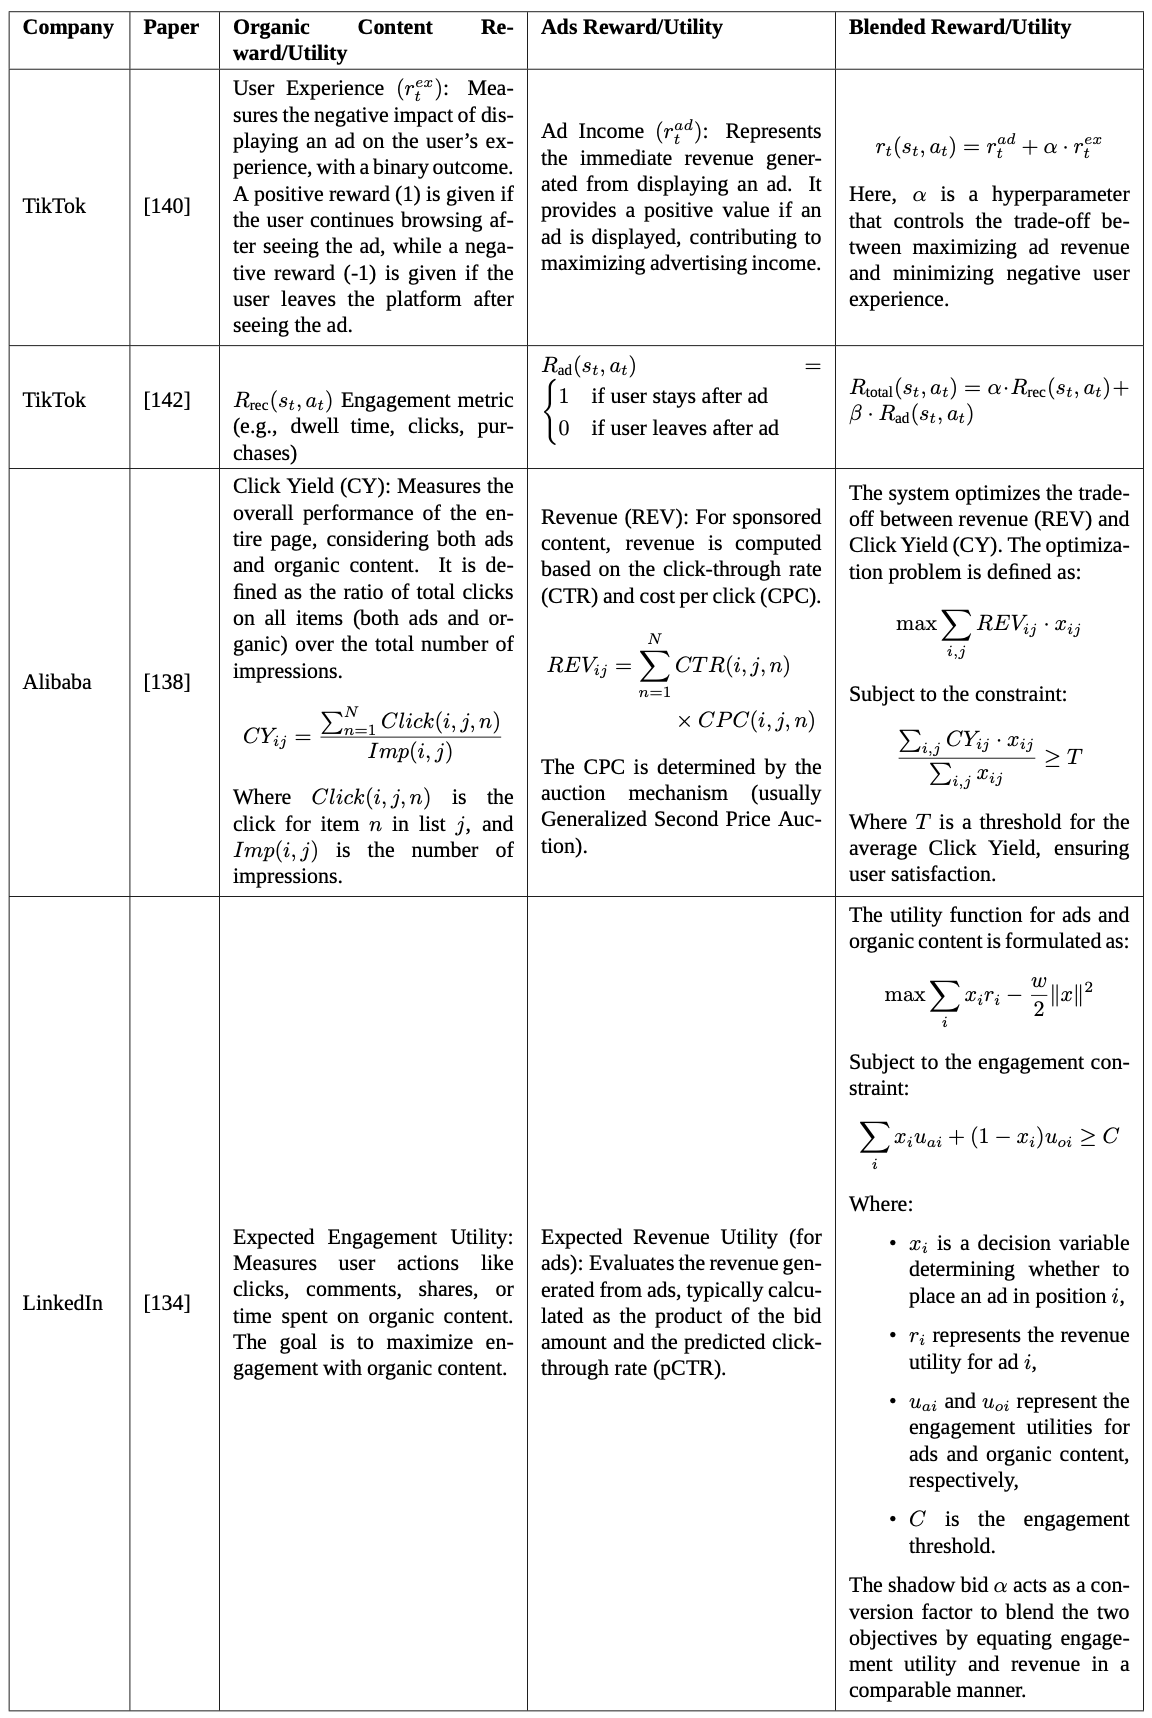
\includegraphics[width=\textwidth, height=0.85\textheight, keepaspectratio]{utility-comparison-table.png}
\caption{Comparison of Utility/Reward Formulation Approaches across Different Companies}
\label{fig:utility-comparison}
\end{figure}



% Adjusted table with better column width control and proper spacing
% \begin{table}[ht]
%     \centering
%     % \renewcommand{\arraystretch}{1.3}  % Adjust row height spacing
%     \begin{adjustbox}{max width=\textwidth}
%     \small % Decrease font size for the table
%     % \setlength{\tabcolsep}{6t} % Increase spacing between text and vertical lines
%     \renewcommand{\arraystretch}{1.15}
% \begin{tabular}{|p{1.5 cm}|p{1 cm}|p{4.5 cm}|p{4.5 cm}|p{4.5 cm}|}
%     \hline
%     \textbf{Company} & \textbf{Paper} & \textbf{Organic Content Reward/Utility} & \textbf{Ads Reward/Utility} & \textbf{Blended Reward/Utility} \\ 
%     \hline
%     TikTok & \cite{zhao2021dear} & 
%     \begin{minipage}{4.5cm}
%     \vspace{4pt}
%         User Experience \((r_t^{ex})\): Measures the negative impact of displaying an ad on the user's experience, with a binary outcome. A positive reward (1) is given if the user continues browsing after seeing the ad, while a negative reward (-1) is given if the user leaves the platform after seeing the ad.
%         \vspace{4pt}
%     \end{minipage}
%     & 
%     \begin{minipage}{4.5cm}
%     \vspace{4pt}
%         Ad Income \((r_t^{ad})\): Represents the immediate revenue generated from displaying an ad. It provides a positive value if an ad is displayed, contributing to maximizing advertising income.
%         \vspace{4pt}
%     \end{minipage}
%     & 
%     \begin{minipage}{4.5cm}
%     \vspace{4pt}
%         \[
%         r_t(s_t, a_t) = r_t^{ad} + \alpha \cdot r_t^{ex}
%         \]
%         Here, \(\alpha\) is a hyperparameter that controls the trade-off between maximizing ad revenue and minimizing negative user experience.
%         \vspace{4pt}
%     \end{minipage} \\
%     \hline
%     TikTok & \cite{zhao2020jointly} & 
%     $R_{\text{rec}}(s_t, a_t)$ Engagement metric (e.g., dwell time, clicks, purchases)  
%     & 
%     \begin{minipage}{4.5cm}
%     \vspace{4pt} 
%     \( R_{\text{ad}}(s_t, a_t) = 
%     \begin{cases} 
%         1 & \text{if user stays after ad} \\
%         0 & \text{if user leaves after ad} 
%     \end{cases} \) 
%         \vspace{4pt}
%     \end{minipage}
%     & 
%     \begin{minipage}{4.5cm}
%     \vspace{4pt}
%     \( R_{\text{total}}(s_t, a_t) = \alpha \cdot R_{\text{rec}}(s_t, a_t) + \beta \cdot R_{\text{ad}}(s_t, a_t) \)
%         \vspace{4pt}
%     \end{minipage} \\
%     \hline
%     Alibaba & \cite{zhang2018whole} & 
%     \begin{minipage}{4.5cm}
%     \vspace{4pt}
%         Click Yield (CY): Measures the overall performance of the entire page, considering both ads and organic content. It is defined as the ratio of total clicks on all items (both ads and organic) over the total number of impressions.
%         \[
%         CY_{ij} = \frac{\sum_{n=1}^{N} Click(i, j, n)}{Imp(i, j)}
%         \]
%         Where \(Click(i, j, n)\) is the click for item \(n\) in list \(j\), and \(Imp(i, j)\) is the number of impressions.
%         \vspace{4pt}
%     \end{minipage}
%     & 
%     \begin{minipage}{4.5cm}
%     \vspace{4pt}
%         Revenue (REV): For sponsored content, revenue is computed based on the click-through rate (CTR) and cost per click (CPC).
%         \[
% \begin{aligned}
% REV_{ij} = \sum_{n=1}^{N} & \, CTR(i, j, n) \\
% & \times CPC(i, j, n)
% \end{aligned}
% \]
%         The CPC is determined by the auction mechanism (usually Generalized Second Price Auction).
%         \vspace{4pt}
%     \end{minipage}
%     & 
%     \begin{minipage}{4.5cm}
%     \vspace{4pt}
%         The system optimizes the trade-off between revenue (REV) and Click Yield (CY). The optimization problem is defined as:
%         \[
%         \max \sum_{i,j} REV_{ij} \cdot x_{ij}
%         \]
%         Subject to the constraint:
%         \[
%         \frac{\sum_{i,j} CY_{ij} \cdot x_{ij}}{\sum_{i,j} x_{ij}} \geq T
%         \]
%         Where \(T\) is a threshold for the average Click Yield, ensuring user satisfaction.
%         \vspace{4pt}
%     \end{minipage} \\
%     \hline
%     LinkedIn & \cite{yan2020ads} & 
%     \begin{minipage}{4.5cm}
%     \vspace{4pt}
%         Expected Engagement Utility: Measures user actions like clicks, comments, shares, or time spent on organic content. The goal is to maximize engagement with organic content.
%         \vspace{4pt}
%     \end{minipage}
%     & 
%     \begin{minipage}{4.5cm}
%     \vspace{4pt}
%         Expected Revenue Utility (for ads): Evaluates the revenue generated from ads, typically calculated as the product of the bid amount and the predicted click-through rate (pCTR).
%         \vspace{4pt}
%     \end{minipage}
%     & 
%     \begin{minipage}{4.5cm}
%     \vspace{4pt}
%         The utility function for ads and organic content is formulated as:
%         \[
%         \max \sum_i x_i r_i - \frac{w}{2} \| x \|^2
%         \]
%         Subject to the engagement constraint:
%         \[
%         \sum_i x_i u_{ai} + (1 - x_i) u_{oi} \geq C
%         \]
%         Where:
%         \begin{itemize}
%             \item \(x_i\) is a decision variable determining whether to place an ad in position \(i\),
%             \item \(r_i\) represents the revenue utility for ad \(i\),
%             \item \(u_{ai}\) and \(u_{oi}\) represent the engagement utilities for ads and organic content, respectively,
%             \item \(C\) is the engagement threshold.
%         \end{itemize}
%         The shadow bid \(\alpha\) acts as a conversion factor to blend the two objectives by equating engagement utility and revenue in a comparable manner.
%         \vspace{4pt}
%     \end{minipage} \\
%     \hline
% \end{tabular}
% \end{adjustbox}
% \caption{Comparison of Utility/Reward Formulation Approaches across Different Companies}
% \label{tab:utility-comparison}
% \end{table}


\subsection{Action Space Representation}
\label{action_space_representation}

In RL, environments are modeled as a Markov Decision Process (MDP). An MDP is defined by $(\mathcal{S}, \mathcal{A}, P, R)$, where $\mathcal{S}$ is the state space, $\mathcal{A}$ is the action space, $P(\cdot\mid s,a)$ is the transition probability distribution, and $R(s,a)$ is the reward function. At each timestep $t$, the agent observes a state $s_t \in \mathcal{S}$ and selects an action $a_t \in \mathcal{A}$. Both action and state sets may be finite, infinite, discrete, or continuous.

% What is an action 
In RL, an \textbf{action} $a \in \mathcal{A}$ refers to \textbf{a decision or intervention taken by the agent based on its current state to influence the environment} \cite{Sutton1998}. The action space $\mathcal{A}$  represents the complete set of all possible actions that the agent can choose from at any given decision point \cite{Sutton1998}. For example, in the  FrozenLake environment,\textbf{ the possible actions for the agent are \textit{up, down, left} and \textit{right}} \cite{frozenlake}. \textbf{Because this set of possible actions is countable, the action space for the FrozenLake is said to be \textit{discrete} \cite{frozenlake}.} By contrast, in an \emph{advertisement recommendation} setting, the action space $\mathcal{A}$ might consist of all possible combinations of ads, their rankings, placements, and formats \cite{ie2019slateq}. The objective of this set of actions in ad recommendation is to deliver the right set of ads at the right time in order to maximize platform revenue, while maintaining or improving user engagement and satisfaction \cite{zhao2020jointly}. Although this action space is discrete and countable, the number of possible combinations grows exponentially with the number of candidate ads and available slots. As a result, it becomes computationally infeasible to enumerate or evaluate each action individually, and must instead be treated using methods designed for high-dimensional discrete spaces \cite{ie2019recsim}.

\textbf{An ideal action space should be \textit{expressive} enough to capture all relevant degrees of freedom the agent needs to optimize its behavior, but it should avoid unnecessary complexity \cite{zhu2024discretizing, liu2025reducing}.} The action space described above in the FrozenLake example satisfies these criteria, as the four cardinal movements (\textit{up, down, left,} and \textit{right}) are enough to navigate to any state in the grid while remaining \textbf{orthogonal}, thus providing both sufficient \textbf{coverage and simplicity} \cite{frozenlake}.  In contrast, the ad recommendation action space is inherently high-dimensional and entangled \cite{ie2019recsim}. The agent must decide \emph{what} to show (a discrete choice over candidate ads), \emph{where} to place it  (which may be modeled as a discrete slot or a continuous position), and in \emph{what order} (often determined by continuous relevance scores), often under tight latency constraints and user personalization requirements \cite{zhao2020jointly}. The action space in ad recommendation systems must be expressive enough to encompass all relevant choices for optimal ad delivery while ensuring no combinatorial explosion in complexity \cite{ie2019slateq}. Moreover, ensuring that each dimension remains sufficiently \emph{orthogonal} can be nontrivial, given potential interactions between ad content, positioning, and user context \cite{ie2019reinforcement}. If the action space is too coarse, the system risks underfitting, serving generic policies that fail to personalize effectively or miss monetization opportunities \cite{ie2019slateq}. On the other hand, if it is too fine, the system may overfit to noise, struggle to generalize, or incur prohibitive computational costs \cite{ie2019slateq}. Practical systems often resort to action abstraction or parameterization (e.g., slate-based policies, ad load knobs, or policy buckets) to reduce complexity at the cost of optimality \cite{ie2019reinforcement, hohnhold2015focusing, sagtani2024ad}.

\textbf{The independence of these action dimensions facilitates more modular policy learning \cite{tavakoli2018action, sharma2017learning}}. By allowing a degree of independence for each action dimension, the agent achieves modular policy learning that scales linearly (instead of exponentially) with the number of action degrees-of-freedom \cite{tavakoli2018action}. In addition, actions should ideally correspond to \textbf{semantically meaningful choices} to facilitate policy interpretability and validation \cite{glanois2024survey, puiutta2020explainable}. In the case of the FrozenLake problem, the action space is intuitive and human-interpretable, making it straightforward to validate learned policies \cite{brockman2016openai, Sutton1998}. For instance, an RL practitioner can manually inspect and reason about the learned policy (e.g. "the agent plans to move \textit{down} then \textit{right} to reach the goal") to verify that each action choice aligns with domain logic \cite{brockman2016openai}. While the action space in ad recommendation systems is far more complex, structuring it around semantically meaningful levers (e.g., “increase ad load for high-intent users” or “downrank low-quality creatives”) enables engineers and product teams to reason about the system’s behavior \cite{glanois2024survey, dulac2021challenges}. If a learned policy increases ad load for a particular user segment, analysts can trace this decision back to upstream signals, such as historical engagement patterns or commercial intent scores \cite{gauci2018horizon, dulac2021challenges}. Policies composed of interpretable levers enable more transparent debugging, offline validation, and policy review, which is crucial for ensuring that the deployed strategy aligns with business intuition, avoids learning spurious correlations, and mitigates the risk of unintended outcomes \cite{dulac2021challenges, verma2018programmatically, puiutta2020explainable, glanois2024survey}.

\textbf{Moreover, an action space should be consistent across episodes \cite{puterman2014markov}.} That is, taking the same action in the same state should yield statistically predictable outcomes \cite{puterman2014markov}. \textbf{The state space in the FrozenLake is stochastic \cite{frozenlake}}, meaning that taking the same action does not always result in the same next state. For example, selecting the action "move right" might result in the agent moving right, up, or down, as governed by the transition probabilities defined by $P(s' \mid s, a)$ \cite{frozenlake}. Despite the stochasticity in the environment,\textbf{ the outcomes observed should converge to the expected values described by the transition probability distribution over a sufficiently large number of episodes \cite{puterman2014markov}}. A similar principle applies in ad recommendation. Although user behavior and auction dynamics introduce stochasticity, \textbf{taking the same ad-serving action, such as presenting a specific slate of ads to a user with a given context, should yield statistically predictable engagement or monetization outcomes}. That is, over many episodes, \textbf{the distribution of observed rewards (e.g., clicks, conversions, revenue) should converge to the expected value associated with the given state-action pair \cite{mcmahan2013ad, zhao2018deep}}. This consistency is foundational for policy learning, as it ensures that repeated exposure to similar decision contexts enables accurate estimation of long-term value, despite noisy observations \cite{Sutton1998}. 

The action space can be thought of as levers that can be used to tune ad policy. Typical \textbf{levers in treatments in ad policies} include the following elements \cite{koutsopoulos2016native}: 

\begin{itemize}
    \item \textbf{Ad Load.} Also referred to as the spacing ads or frequency of ads is also a key component in inducing ad load fatigue. Placing ads too closely together may lead to user fatigue and reduced click probabilities \cite{abrams2007personalized, zhao2020jointly}. 
    \item \textbf{Ad Quality.} This refers to intrinsic features of the ad, such as the design format, product type, accompanying text, and the quality of the landing page, all of which directly influence user engagement. \cite{yan2009much, nielsen2017advertising}.
    \item \textbf{Ad Placement.}
Ads placed earlier in the feed are more likely to be clicked, though their relevance to preceding content also plays a significant role \cite{zhao2020jointly, saha2021advertiming, yuan2020unbiased}. 
    \item \textbf{Ad Relevance.} Ads that align more closely with user preferences and user intent are more likely to drive engagement. For example, an ad on a hotel might have a higher probability if shown adjacent to results of search queries related to vacations \cite{chakrabarti2008contextual, Zhou2018}. \\
\end{itemize}

\subsection{State Space Representation} \label{state_space_representation}
% Definition and Desirable Properties
% 1.1 What is a state space in RL?
% 1.2 Desirable properties of a state space
% Markovianity
% Expressiveness vs. generalization
% Stability under distribution shift
% Sample efficiency and learnability
% Interpretability and support for counterfactual reasoning

In RL, a \textit{state} $s \in \mathcal{S}$  represents all the relevant information from past agent-environment interactions necessary for the agent to make optimal decisions to maximize the expected cumulative reward \cite{Sutton1998}. Ideally, the state space is Markovian, meaning the future is conditionally independent of the past given the current state \cite{russell2016artificial, Sutton1998}. If the agent’s policy or value estimates rely on omitted or unobserved information from the past, the state representation violates the Markov property and the performance of the learned policy may degrade as a result \cite{russell2016artificial, Sutton1998}. In the FrozenLake example, the state space consists of the agent’s current grid position as the future outcomes of any action depend only on this position, and not on how the agent arrived there \cite{frozenlake}. In this example, because future transitions depend only on the current state and action, and not on prior history, the FrozenLake Environment satisfies the \textit{Markov Property} \cite{Sutton1998, frozenlake}.  


In contrast, the environments where \textbf{ad recommendation systems} operate are often \textbf{partially observable, high-dimensional, and non-stationary} \cite{dulac2021challenges, russell2016artificial}. To construct a state representation that reasonably approximates the Markov property in the face of partial observability and complex user dynamics, ad recommendation systems often combine tabular features with learned embeddings \cite{afsar2022reinforcement, kaelbling1998planning}. The tabular signals tend to include static attributes (e.g. demographics), contextual metadata (e.g. device type, time of the day), and behavioral history (e.g. recent clicks, impressions, or dwell time) \cite{cheng2016wide, covington2016deep}. An embedding is a learned, dense vector that encodes complex or high-cardinality inputs, such as user profiles, ads, or behavioral sequences, into a lower-dimensional space \cite{cheng2016wide}. Compared to static tabular features like frequency counts or recency buckets, embeddings capture richer structure, including sequence effects and latent similarity. This makes them more expressive and task-relevant, enabling ad recommendation systems to personalize content and ads more effectively \cite{covington2016deep, cheng2016wide}.

% User embeddings, item embeddings, user-item interaction embeddings, and sequence embeddings are among the most common embedding types used in recommendation systems. Each embedding type captures distinct aspects of information to guide the agent’s decisions. 

% Contextual features, including a user's location or device type, often serve as informative priors, particularly helpful in addressing the cold-start problem, i.e., when new users enter an ecosystem with limited historical data \cite{covington2016deep}. Additionally, some platforms prompt new users to select interests or topics during onboarding, providing supplementary signals that help initialize user embeddings. When no data for users is available (incognito window, SEO-driven traffic, new device without login, etc), systems typically default to population-level trends or popular content. While user embeddings may also be static and updated on batch mode, user embeddings can also be updated dynamically, such that as users engage further, the continuous updates on the embeddings allow for more personalized policies by the agent to reflect new information in the system and evolving preferences.

Embeddings may consist of two components: an offline (stationary) component and an online (non-stationary) component \cite{zhao2023embedding}. \textbf{Offline embeddings} represent \textbf{stationary or slow-changing attributes}, such as a user's demographics (e.g., gender, country) or long-term preferences, and fixed item properties (e.g., brand or product category) \cite{koren2009matrix, quadrana2018sequence}. These embeddings are usually computed in batch mode due to their \textbf{higher computational complexity, larger size, and relatively static nature} \cite{naumov2019deep, liu2022monolith}. \textbf{Online embeddings}, conversely, address non-stationary and rapidly evolving aspects such as recent user behaviors, trending content, or immediate interests \cite{Zhou2018, zhou2019deep}. These embeddings are \textbf{generally smaller,} \textbf{computed in near-real-time to meet latency requirements} \cite{liu2022monolith}. This hybrid approach combines stable and dynamic embeddings, balancing relevance with computational efficiency \cite{cheng2016wide, covington2016deep}. Furthermore, this allows the recommendation system to remain stable under distribution shifts, which is of paramount importance, especially in environments with rapidly evolving user preferences, content inventories, and behavioral patterns \cite{gama2014survey, Sutton1998}.

To effectively integrate diverse embeddings (user, item, interaction) and their offline and online components, embeddings of varying dimensions are typically concatenated and then projected via learned linear layers into a shared dimension \cite{pancha2022pinnerformer, grbovic2018real, covington2016deep}. Generally, zero-padding or truncation is avoided, as these methods can introduce noise or cause information loss \cite{xia2023transact}.

\textbf{User embeddings} are learned vector representations designed to capture user preferences and behaviors, enabling ad recommendation systems to personalize content effectively at scale \cite{covington2016deep, he2017neural}. These embeddings compress complex, high-dimensional user data, such as past interactions and demographic information, into compact vectors utilized by recommendation models \cite{covington2016deep, koren2009matrix, naumov2019deep}. User embeddings can be learned using a combination of supervised, unsupervised, and self-supervised approaches \cite{zhao2021dear}.  In the case of supervised learning, embeddings are optimized to predict explicit labels such as clicks, conversions, or purchases \cite{covington2016deep, Zhou2018}. To exploit information in more implicit signals, self-supervised methods can be used with objectives such as next item interaction or item co-occurrence \cite{yuan2020unbiased, mikolov2013distributed}. Many practical implementations tend to combine both supervised and self-supervised methods \cite{zhao2021dear, xia2023transact}. For example, embeddings may initially be learned through self-supervised tasks (e.g., predicting next clicks) and then fine-tuned on supervised tasks (CTR, conversions). A well-documented example is that of YouTube, where despite the availability of explicit feedback mechanisms (thumbs up/down, in-product surveys, etc.), they turn to implicit signals, where a user completing a video is a positive example, given that the relative prevalence of implicit signals is much higher than explicit signals, allowing the models to learn more effectively \cite{covington2016deep}.

\textbf{Item embeddings} are designed to capture intrinsic item characteristics \cite{koren2009matrix}. These embeddings compress complex, high-dimensional item data, such as product descriptions, categories, brands, and historical interaction patterns \cite{koren2009matrix, cheng2016wide}. Similar to user embeddings, item embeddings can be learned through supervised, unsupervised, and self-supervised approaches \cite{barkan2016item2vec, zhao2023embedding}. In supervised learning scenarios, embeddings are optimized to predict explicit labels, such as clicks, conversions, or purchases associated with the items \cite{covington2016deep, naumov2019deep}. To leverage more implicit information, self-supervised methods may focus on objectives like predicting co-occurrence patterns or sequential interactions (e.g., item-to-item relationships) \cite{barkan2016item2vec, sun2019bert4rec}. 

While user and item embeddings provide essential representations of individual entities, it is through interaction embeddings, which capture the joint dynamics between users and items, that the system truly learns user preferences and can surface content that is contextually relevant and personalized \cite{koren2009matrix}. Being able to \textbf{ effectively represent user-item interactions} is at the core of personalization for recommendation systems \cite{linden2003amazon}. Collaborative Filtering (CF) was one of the earliest popular methods to represent user-item interactions \cite{linden2003amazon, Bobadilla2013}. CF predicted user preferences by analyzing explicit interactions (e.g., ratings) or implicit behavioral signals (e.g., clicks, views), using metrics like cosine similarity or Pearson correlation \cite{Bobadilla2013}. However, CF struggled with sparse datasets, as many user-item pairs lacked interactions, limiting recommendation accuracy \cite{Bobadilla2013}. Additionally, CF's direct interaction-based approach limited its ability to capture deeper latent or implicit relationships between users and items \cite{koren2008factorization}.

Matrix Factorization (MF), popularized during the Netflix Prize competition (2006–2009), addressed some of CF’s key limitations \cite{bennett2007netflix}. The classic approach is to factorize the (sparse) interaction matrix into the product of a user-factor matrix and an item-factor matrix \cite{koren2009matrix}. MF learns these latent (hidden) user and item factors by optimizing embeddings to reconstruct observed interactions, enabling it to capture deeper relational structures that CF missed \cite{koren2009matrix}. MF also significantly improved storage efficiency \cite{koren2009matrix}. For instance, a CF matrix with 1 million users and 1 million items would contain 1 trillion (mostly sparse) entries. In contrast, MF represents these interactions using two dense embedding matrices totaling approximately 128 million entries (assuming an embedding dimension of k=64) \cite{koren2009matrix}.

As companies began logging large-scale user interaction data in the late 2000s and early 2010s, Amazon, Spotify, and Netflix turned to Matrix Factorization (MF) as a simple yet effective way to harness that data for scalable personalization \cite{gomez2015netflix, linden2003amazon}. However, while MF improved predictions for existing users/items with limited interactions, it did not solve all limitations of CF \cite{koren2009matrix}. Particularly, MF still struggled with the cold-start problem, as completely new users or items without interaction history cannot be effectively represented in the embedding space \cite{koren2009matrix}. Additionally, MF assumes linear interactions between latent factors, limiting its ability to capture more complex, nonlinear user behaviors \cite{he2017neural}. Neural embeddings emerged in the 2010s to address some of these limitations \cite{he2017neural}. Unlike CF and MF, neural embeddings naturally capture complex, nonlinear interactions between users and items \cite{he2017neural}. They also effectively incorporate content-based and contextual metadata, significantly improving the handling of cold-start issues \cite{van2013deep, cheng2016wide, naumov2019deep}. Two-tower models,  notably introduced by Google for YouTube’s recommendation systems, leverage deep neural networks for scalable candidate retrieval and generation \cite{covington2016deep}.  A two-tower model consists of two distinct neural network components: one tower encodes user-specific features, and the other one encodes item-specific features, projecting them into a shared latent embedding space \cite{covington2016deep}. This shared embedding space enables efficient similarity computation, facilitating large-scale real-time recommendations \cite{covington2016deep}. Today, companies like YouTube use two-tower models for tasks such as next-video prediction, and Meta uses them for personalized ad ranking \cite{covington2016deep, he2014practical, naumov2019deep}.

Following the widespread adoption of two-tower neural networks, the need to explicitly capture temporal dynamics emerged, motivating the rise of sequence-aware embeddings \cite{quadrana2018sequence}. Users’ preferences evolve continuously, and earlier methods struggled to effectively capture these dynamics \cite{gama2014survey}. Earlier embedding methods, such as Matrix Factorization and two-tower models, primarily represented user-item relationships statically, without adequately capturing evolving user preferences or the order of interactions \cite{koren2009matrix, covington2016deep}. Sequence-aware embeddings thus emerged as an important advancement \cite{quadrana2018sequence}. Initially, RNNs, particularly GRUs, were introduced to model sequential user behaviors \cite{kang2018sasrec}. GRUs could effectively capture short-term temporal dependencies by processing sequences step-by-step, making them well-suited for real-time recommendation tasks \cite{kang2018sasrec, zhao2021dear}. However, these recurrent architectures faced several key limitations: they were prone to the vanishing gradient problem, where information from earlier interactions diminished during training, making it challenging to capture long-range dependencies \cite{Bengio1994}. They also exhibited a recency bias, disproportionately emphasizing recent interactions and overlooking longer-term user interests \cite{Pascanu2013}. Moreover, their sequential nature resulted in slow training times, limiting their scalability \cite{shim2022comparison}. To address these limitations, Transformers, originally introduced by Vaswani et al. in 2017, became widely adopted for recommendation tasks in the late 2010s and early 2020s \cite{vaswani2017attention}. Transformers leveraged self-attention mechanisms, allowing the model to simultaneously process all interactions in a sequence and dynamically attend to the most informative interactions—such as pivotal clicks, conversions, or moments of high engagement \cite{vaswani2017attention}. This adaptive attention mechanism effectively mitigated the vanishing gradient problem, robustly captured both short-term and long-range dependencies, and reduced recency bias by emphasizing interactions based on relevance rather than mere chronological proximity \cite{kang2018sasrec, vaswani2017attention}. 

Transformers enable parallel processing over sequence elements, significantly accelerating training and making them well-suited for large-scale recommendation systems with extensive historical data \cite{vaswani2017attention, kang2018sasrec}. Industry models like Pinterest’s PinnerFormer (2020) and ByteDance’s DEAR (2021) have leveraged this capability to effectively model evolving user behavior and serve contextually relevant recommendations \cite{pancha2022pinnerformer, zhao2021dear}.

\subsection{Policy Learning} \label{policy_learning}

A policy is a core component of any RL system \cite{Sutton1998}. It encodes not only the logic that determines which action the agent should take in a given state to maximize long-term cumulative rewards, but also how much to explore versus exploit \cite{Sutton1998, russell2016artificial}. Exploration is necessary for the agent to discover the value of unfamiliar actions, which may lead to better strategies \cite{russo2018tutorial}. However, this must be balanced with exploitation, which involves choosing actions that are already known to yield high rewards \cite{auer2002finite}. Without a policy, the agent has no systematic way to select actions or improve its behavior based on feedback from the environment \cite{Sutton1998}.

Formally, a policy is denoted as $\pi(a|s)$, representing the probability of selecting action $a$ given state $s$ \cite{Sutton1998, russell2016artificial}. In the context of the FrozenLake example, a policy is the mapping of grid positions (e.g. the states) to the optimal moves {\textit{up, down, left, right}} (e.g the actions) in order to maximize cumulative reward \cite{frozenlake}. The FrozenLake setting also provides intuition for the explore–exploit tradeoff \cite{frozenlake}. If the agent only explores, it never settles on a reliable strategy and may keep falling into holes \cite{Sutton1998}. If it only exploits, it might stick to a suboptimal path and miss shorter or safer routes \cite{russo2018tutorial}. Balancing both is essential to finding the optimal policy \cite{auer2002finite}.

\textbf{The degree of randomness in a policy is an important consideration \cite{Sutton1998}.} A policy can be either stochastic or deterministic \cite{Sutton1998}. In a \textbf{\textit{stochastic} policy}, $\pi(a|s)$ defines a probability distribution over the action space: $\sum_a \pi(a|s) = 1$ and $0 \leq \pi(a|s) \leq 1$ for all $a$ \cite{Sutton1998}. In a \textbf{\textit{deterministic} policy}, the agent always selects the same action in a given state, with $\pi(a|s) = 1$ for exactly one action and $0$ for all others \cite{puterman2014markov}. A deterministic policy can be expressed as $\pi(s) = a$, where, in the context of the FrozenLake example, $s$ is the agent’s current position in the grid and $a$ is the action selected from the set \{\textit{up}, \textit{down}, \textit{left}, \textit{right}\} \cite{frozenlake}. For example, if $\pi((2,1)) = \textit{down}$, it means that when the agent is in row 2, column 1 of the grid, it should move down to maximize the expected return \cite{FrozenLakeGymnasium2023}.

\textbf{It is important to distinguish between the stochasticity of the \textit{policy} and that of the \textit{environment}} \cite{Sutton1998}. A policy determines which action the agent selects in a given state \cite{Sutton1998, russell2016artificial}. The environment, by contrast, is modeled by transition dynamics that specify a probability distribution over the next state and reward, given the current state and action \cite{puterman2014markov}. This is typically denoted as \( P(s', r \mid s, a) \), where \( s \) is the current state, \( a \) is the selected action, and \( (s', r) \) is the resulting next state and reward \cite{Sutton1998, puterman2014markov}. However, while the decision of choosing the action of \textit{moving right} given a state may be deterministic, what happens next is subject to the degree of stochasticity present in the environment \cite{Sutton1998, FrozenLakeGymnasium2023}. Due to slipperiness, taking the action to move  'right' from that cell may result in the agent actually moving in a different direction, such as \textit{up} or \textit{down}, each with some probability \cite{frozenlake}. Thus, an agent can act deterministically in an environment where the outcomes of its actions are probabilistic \cite{Sutton1998, kaelbling1996reinforcement}.

The \textbf{optimal policy $\pi^*$} is the one that maximizes the expected cumulative return from any given state \cite{Sutton1998, puterman2014markov}. In Markov Decision Processes (MDPs), this is often expressed as 
\begin{equation}
\pi^*(a|s) = \arg\max_{\pi} \mathbb{E} \left[ \sum_{t=0}^{\infty} \gamma^t r_t \,\middle|\, \pi, s_0 = s \right]
\end{equation}
where $\gamma \in [0,1)$ is the discount factor and $r_t$ is the reward received at time $t$ \cite{puterman2014markov, Sutton1998}.

This simplicity in defining states, actions, transitions, and rewards makes toy examples like GridWorld ideal for illustrating core RL concepts, but they lack the complexity and ambiguity found in real-world applications, where the state space is vast, the actions are numerous and continuous, and the rewards are often delayed and difficult to quantify \cite{dulac2021challenges, levine2020offline}, .

In the context of \textbf{ad policy optimization}, the policy $\pi(a|s)$ defines how the system selects ads $a$ to display to a user in a particular state $s$, using levers such as ad load, placement, and price thresholds, as detailed in Section~\ref{action_space_representation} \cite{zhang2018whole, zhao2021dear, ie2019reinforcement}. The state $s$ may include the user’s profile, browsing history, session context, and inferred commercial intent, as discussed in Section~\ref{state_space_representation} \cite{pancha2022pinnerformer, xia2023transact, Zhou2019}. The policy can be deterministic (always show the same ad for a given state) or stochastic (show ads based on probabilities) \cite{Sutton1998, levine2020offline}. In advanced recommendation systems, ad policies are typically stochastic, whereas in older recommendation systems, policies might be deterministic (i.e. every X impressions of organic items show ad Y from list Z) \cite{gauci2018horizon, zhao2021dear}.  \textbf{Stochastic policies} are desirable because they \textbf{naturally support exploration}, allowing the system to sample from a range of actions rather than always selecting the historically best-performing one \cite{Sutton1998, russo2018tutorial}. This \textbf{helps avoid local optima} and uncover ad-user pairings that may lead to better long-term outcomes \cite{zou2019reinforcement, mazoure2021improving}. Moreover, stochastic policies provide a practical mechanism for managing uncertainty and partial information \cite{dulac2021challenges, levine2020offline}. When it is unclear which action best serves all objectives, such as monetization and long-term engagement, randomizing over plausible actions allows the system to spread risk and continue learning \cite{Mehrotra2020, Jannach2023}. While \textbf{deterministic policies} can in principle encode complex tradeoffs, they may hard-code assumptions that \textbf{ do not generalize well or require re-tuning as user behavior shifts }\cite{dulac2021challenges}. Stochastic policies, by contrast, can naturally adapt via probabilistic weighting as more data becomes available \cite{levine2020offline, gauci2018horizon}.


\textbf{Learning a policy} involves a series of critical design decisions that must account for both \textbf{algorithmic trade-offs and real-world constraints}. These include whether to learn from historical data in an \textbf{offline} setting or through direct interaction with the environment via \textbf{online learning}; whether to rely on \textbf{value-based methods} \textbf{or policy-based optimization}; whether to incorporate an \textbf{explicit model of the environment or adopt a model-free approach}; and whether to use \textbf{tabular methods or generalize through function approximation}. In addition, selecting an appropriate \textbf{exploration} strategy is essential for balancing the trade-off between learning new behaviors and \textbf{exploiting} known high-reward actions. This section provides guidance on how to navigate these decisions, using the FrozenLake environment as a conceptual reference point and highlighting real-world implementations from large-scale recommendation systems.

\subsubsection{Offline vs Online Policy Learning}
Depending on whether the agent learns by training on historical data or by interacting with the environment in real time,  \textbf{policy learning can be categorized as either offline or online \cite{Sutton1998}}. \textbf{In offline policy learning, }models are trained using logged data from past user interactions, without actively modifying the live system \cite{levine2020offline}. This is often the safest and most scalable approach in large platforms, as it avoids the risk of deploying untested policies \cite{levine2020offline}. Offline methods are particularly useful during the early stages of development when real-time exploration is expensive \cite{levine2020offline, gauci2018horizon, Mehrotra2020}. 

Monte Carlo (MC) methods estimate the expected return of a policy by averaging cumulative rewards across complete episodes of logged interactions \cite{Sutton1998, levine2020offline}. Because they require observing full trajectories before updates, MC methods are particularly well-suited to settings where rewards are delayed and live exploration is costly \cite{Sutton1998, levine2020offline}. This makes them a natural fit for early-stage offline learning scenarios, where the focus is on extracting long-term value insights from existing data without interacting with the live environment \cite{Sutton1998, levine2020offline}. However, Monte Carlo methods have notable limitations \cite{Sutton1998}. Waiting for full episodes to complete can make them highly sample-inefficient, particularly in environments where episodes are long or rewards are sparse \cite{levine2020offline}. This inefficiency can delay policy improvements and slow adaptation to changes \cite{dulac2019challenges}. Furthermore, MC estimates often suffer from high variance, especially in noisy or stochastic environments, which can destabilize learning unless techniques like reward normalization, batch averaging, or variance reduction are applied \cite{Sutton1998}. Monte Carlo approaches also assume that logged episodes are representative of the environment; if the logging policy is narrow or biased, importance sampling corrections become necessary to avoid skewed estimates \cite{swaminathan2015counterfactual}. Due to these limitations, Monte Carlo methods are typically not used in high-frequency online systems where quick updates are critical \cite{dulac2019challenges}. As an illustrative example of offline learning, in the context of the FrozenLake environment, offline policy learning refers to the process of learning a policy using a log of past episodes, i.e. sequences of (state, action, next state, reward) generated by a prior policy.  The learner must rely entirely on the logged data to reason about optimal behavior in navigating from the start state (S) to the goal (G), while avoiding holes (H) and dealing with slippery transitions. 

\textbf{Logged data only contains actions chosen by the historical policy}, which means there is no direct visibility into what would have happened if alternative actions had been taken in the same context \cite{swaminathan2015counterfactual}. This \textbf{lack of counterfactual information makes it difficult to evaluate or iterate on new policies \cite{dudik2011doubly}}. However, methods such as inverse propensity scoring (IPS), which re-weights logged rewards to approximate outcomes under a different policy, and doubly robust estimators, which combine IPS with model-based value predictions, can help address this challenge \cite{swaminathan2015counterfactual, dudik2011doubly, levine2020offline}. These approaches enable limited forms of counterfactual reasoning, especially when the new policy does not diverge too far from the one that generated the data \cite{swaminathan2015counterfactual, dudik2011doubly}. 

A simple example of counterfactual estimation being viable in the FrozenLake environment can be illustrated as follows: suppose the agent has never made a left turn from state 4. While we may not have logged data on this specific action at this specific grid location, a function approximator—such as a neural network trained over state-action pairs—might still be able to infer the expected outcome. This is because the model could have learned to generalize from similar patterns observed in nearby states, allowing it to estimate the return of an unobserved action in a plausible way \cite{levine2020offline, dudik2011doubly}.

To overcome the constraints of limited exploration in offline settings, \textbf{online policy learning enables agents to refine their policies by interacting with the environment and learning from new experiences} \cite{dimitrakakis2018decision}. The agent is able to explore different actions, observe the consequences in real time, gather feedback, and update its behavior accordingly. This ability to learn directly through interaction with the environment makes online learning more flexible and adaptive, although it also introduces greater risk \cite{dulac2019challenges}. 

To mitigate risks and costs of online exploration, offline is almost always used first \cite{levine2020offline}. Online is introduced gradually via controlled bandit loops, feature gates, or soft rollouts. This hybrid approach of offline-then-online policy learning is commonly seen in industry. In their offline RL system, YouTube trained an actor-critic model entirely on logged user interaction data, using Monte Carlo returns to estimate long-term value, and only deployed policies to production after thorough offline evaluation \cite{chen2022off}. At Meta, the Horizon platform first trains policies offline using counterfactual estimators like Doubly Robust evaluation, and then deploys them through gated rollouts, which refer to the controlled and staged release of new policies to a limited portion of traffic in order to minimize risk during online learning \cite{gauci2018horizon}. Spotify similarly adopts a cautious approach by first optimizing contextual bandit policies offline, and then introducing online learning through incremental updates and careful exploration strategies \cite{Mehrotra2020}.

\subsubsection{Value-based vs Policy-based Learning}

RL algorithms can be divided into value-based and policy-based methods based on how they learn to make decisions to maximize cumulative rewards \cite{Sutton1998, russell2016artificial}. Value-based methods first estimate the value of states or state-action pairs and then derive a policy from these estimates, whereas policy-based methods learn the policy directly by optimizing expected cumulative reward \cite{Sutton1998, schulman2017proximal}. In other words, value-based methods focus on learning the utility of states or actions and derive the optimal behavior indirectly by acting greedily with respect to this learned value \cite{Sutton1998}. Policy-based methods, in contrast, directly optimize the policy without estimating value functions \cite{Sutton1998, schulman2017proximal}. 

There are two common \textbf{value functions}. The first is the state value function, defined as
    \begin{equation}
        V^{\pi}(s) = \mathbb{E}_{\pi} \left[ \sum_{t=0}^{\infty} \gamma^t R_{t+1} \,\middle|\, S_0 = s \right]
        \label{eq:v_function}
    \end{equation}
    which gives the expected return when starting in state $s$ and following policy $\pi$ thereafter. As in standard RL notation, \( R_{t+1} \) is the reward received at time step \( t+1 \), and \( \gamma \in [0, 1] \) is the discount factor that determines how much future rewards are valued relative to immediate ones. The lower the value of $\gamma$, the less future rewards influence the total return \cite{Sutton1998, russell2016artificial}. The second is the action value function, defined as
    \begin{equation}
        Q^{\pi}(s, a) = \mathbb{E}_{\pi} \left[ \sum_{t=0}^{\infty} \gamma^t R_{t+1} \,\middle|\, S_0 = s, A_0 = a \right]
        \label{eq:q_function}
    \end{equation}
which gives the expected return when starting in state $s$, taking action $a$, and then following policy $\pi$ \cite{Sutton1998, russell2016artificial}. Once the action-value function \( Q(s, a) \) is learned,  the agent can act greedily with respect to its current value estimates by selecting the action that maximizes this function:

\begin{equation}
    \pi(s) = \arg\max_a Q(s, a)
    \label{eq:greedy_policy}
\end{equation}

where \( \pi(s) \) denotes the policy derived from the current value function \cite{Sutton1998}. This approach allows the agent to act greedily with respect to its current value estimates, that is, to select the action that appears to yield the highest expected return at the next decision point, gradually improving its behavior as the value function becomes more accurate \cite{Sutton1998}. Because value-based methods rely on greedy action selection to determine the next best action, they require comparing the estimated value of all possible actions at each decision point (e.g. each state) \cite{Sutton1998, dulac2019challenges}. As the number of available actions grows, and as the agent encounters more states during interaction, this exhaustive comparison becomes computationally intractable \cite{dulac2019challenges}. For this reason, value-based methods are particularly well-suited for environments with discrete or low-dimensional action spaces, where enumerating and comparing action values remains computationally feasible \cite{dulac2019challenges, Sutton1998}. Common algorithms used in value-based learning include Q-learning, SARSA, and Deep Q-Networks (DQN) \cite{Sutton1998, mnih2015human}. 

\textbf{In Policy-based learning}, the agent tries out different strategies and tweaks their behavior directly based on what works well overall, rather than scoring every possible move \cite{russell2016artificial, Sutton1998}. Formally, the goal is to learn a parameterized policy \( \pi_\theta(a \mid s) \), where \( \theta \) denotes the parameters of the policy \cite{Sutton1998, schulman2017proximal}. In practice, especially in modern industrial applications, these parameters are often the weights of a neural network, though other function approximators are possible \cite{Sutton1998, levine2020offline, mnih2016asynchronous}. Neural network-based policies have become the norm in large-scale recommendation systems due to their expressiveness and scalability, making them particularly well-suited for environments with complex and high-dimensional state spaces \cite{lin2023survey, chen2022off, gauci2018horizon}. Formally, the objective function to be maximized is the expected cumulative reward under the policy: 
\begin{equation}
    J(\theta) = \mathbb{E}_{\tau \sim \pi_\theta} \left[ \sum_{t=0}^{\infty} \gamma^t R_{t+1} \right]
    \label{eq:objective_function}
\end{equation}
where \( \tau \) denotes a trajectory: a sequence of states and actions generated by following the policy \( \pi_\theta \) \cite{Sutton1998, levine2020offline}. To optimize this objective, the policy gradient theorem provides a way to compute the gradient of the expected return with respect to the policy parameters, given by:

\begin{equation}
    \nabla_\theta J(\theta) = \mathbb{E}_{\pi_\theta} \left[ \nabla_\theta \log \pi_\theta(a \mid s) \cdot Q^{\pi_\theta}(s, a) \right]
    \label{eq:policy_gradient}
\end{equation}

where \( Q^{\pi_\theta}(s, a) \) is the action-value function under the current policy \cite{Sutton1998, williams1992simple}. Since the goal is to maximize return, gradient ascent, not descent, is used \cite{Sutton1998, williams1992simple}. \textbf{Common policy-based RL algorithms }include REINFORCE, Proximal Policy Optimization (PPO), Trust Region Policy Optimization (TRPO), and various Actor-Critic methods, which \textbf{combine both policy and value learning in a hybrid architecture} \cite{williams1992simple, schulman2015trust, schulman2017proximal, Sutton1998}.

In theory, either value-based or policy-based learning is sufficient to solve an RL problem \cite{Sutton1998, kaelbling1996reinforcement}. However, policy-based methods tend to be more suitable for ad policy optimization for a number of reasons \cite{chen2022off, gauci2018horizon}. \textbf{First, policy-based methods are preferred in scenarios where stochastic policies are desired} because they explicitly parameterize the policy as a probability distribution over actions, rather than implicitly choosing a single best action \cite{williams1992simple, Sutton1998}. What policy-based methods learn are the stochastic policy   $\pi_\theta(a \mid s)$ directly, whereby the output is itself a probability distribution (e.g. softmax over action logits, Gaussian in continuous space) \cite{Sutton1998, schulman2015trust}. \textbf{Moreover, policy-based methods are also desirable when careful tuning of exploration-exploitation is required}, as they can learn when and how to be random, whereas value-based methods cannot \cite{Sutton1998, williams1992simple, schulman2015trust}. In contrast, because value-based methods learn the action-value function $Q(s,a)$ and then derive the deterministic policy $\arg\max_a Q(s, a)$, value-based methods cannot directly represent probability distributions over actions \cite{Sutton1998, dulac2019challenges}. To accommodate for stochasticity, value-based methods resort to $\epsilon$-greedy approaches, which are ad hoc and not a learned methodology \cite{Sutton1998, kaelbling1996reinforcement}. \textbf{Finally, Policy-based methods are often used when we want to optimize a policy across an entire ML pipeline}\cite{Sutton1998, chen2022off}. It is common for ad-ranking systems to start with a transformer-based encoder for ad retrieval and to conclude with a multi-head attention blending layer that predicts a downstream action, where end-to-end differentiability is required to allow the gradient to flow and therefore learn a cohesive policy \cite{zhao2021dear, xia2023transact, pancha2022pinnerformer}. This is difficult to achieve with value-based methods, which estimate a value function \(Q(s, a)\) and then select actions via \(\arg\max_{a} Q(s, a)\) \cite{Sutton1998, dulac2019challenges}. Because \(\arg\max\) is non-differentiable, it breaks gradient flow in neural networks \cite{Sutton1998, dulac2019challenges}. In contrast, policy-based methods directly parameterize the policy \(\pi_\theta(a \mid s)\) using differentiable functions (e.g., softmax or Gaussians) \cite{Sutton1998, williams1992simple}. As a result, gradients can backpropagate through the entire pipeline, from the final action probabilities to earlier neural layers, enabling a fully integrated, end-to-end approach that can incorporate embeddings, attention mechanisms, and encoder-decoder architectures \cite{chen2022off, zhao2021dear, xia2023transact}.

While policy-based methods are powerful and overcome many of the limitations of value-based methods, \textbf{policy-based methods also have their shortcomings} \cite{Sutton1998, levine2020offline}. Policy-based methods assume that the performance of the gradient can be accurately estimated and optimized through sampling \cite{williams1992simple, Sutton1998}. However,\textbf{ these estimates often suffer from high variance}, which can lead to unstable learning and slow convergence \cite{Sutton1998, schulman2015trust}. Because of the absence of an explicit value function, policy-based methods tend to require a larger number of samples compared to value-based methods, making them \textbf{less sample-efficient} \cite{levine2020offline, dulac2019challenges}. \textbf{To overcome these limitations, many large-scale production systems adopt hybrid approaches that combine both value-based and policy-based learning, most notably in the form of actor-critic architectures} \cite{Sutton1998, chen2022off, gauci2018horizon}. In these methods, \textbf{the actor is responsible for learning the policy}, \textbf{while the critic estimates the value function to guide and stabilize the policy updates} \cite{Sutton1998, williams1992simple}. This combination improves learning stability, speeds up convergence, and enhances interpretability, making it well-suited for complex, real-world applications such as recommendation and ad-serving systems \cite{chen2022off, gauci2018horizon, dulac2019challenges}.

To illustrate the \textbf{distinction between value-based and policy-based methods in a simple example, consider the FrozenLake environment} \cite{frozenlake}. In a value-based approach, the agent learns a state-action value function \( Q(s, a) \) that estimates the expected cumulative reward for each action at every grid position \cite{Sutton1998, kaelbling1996reinforcement}. Once trained, the agent derives its policy by selecting the action with the highest value in each state \cite{Sutton1998}. For example, from a particular icy tile near a hole, it may learn that moving right has a higher expected return than moving down, based on accumulated experience. In contrast, a policy-based agent would directly learn a parameterized policy \( \pi(a \mid s) \) that outputs a probability distribution over actions for each state \cite{Sutton1998, williams1992simple}. Instead of estimating the value of each action, it adjusts its parameters to increase the likelihood of action sequences that successfully reach the goal \cite{williams1992simple, Sutton1998}. Over time, this agent may learn, for instance, that taking a probabilistic mix of "right" and "down" from a slippery tile leads to more consistent success, even if it cannot explicitly quantify the expected value of each option.

\textbf{The value-based vs policy-based taxonomy offers a useful lens for categorizing RL approaches in ad policy optimization, based on how decisions are learned to maximize cumulative rewards} \cite{Sutton1998, zhao2021dear, lin2023survey}. \textbf{Platforms like LinkedIn and Google Ads have applied value-based approaches like Q-learning to optimize between discrete ad policies}, such as selecting between low or high ad load treatments, by estimating the expected value of each action for a given user segment \cite{mcmahan2013ad, Theocharous-2015, zhao2024survey}. \textbf{Value-based learning works well when the action space is discrete, small, and easily enumerable}, allowing the agent to derive a policy through the maximization of the learned Q-function \cite{Sutton1998, dulac2019challenges}. \textbf{In contrast, policy-based approaches are better suited for continuous, high-dimensional, or unstructured decision spaces} \cite{Sutton1998, dulac2019challenges, schulman2015trust}. While industry examples above from Google and LinkedIn have applied value-based methods such as Q-learning to optimize among a small set of discrete ad policies (e.g., choosing between high and low ad load treatments) \cite{mcmahan2013ad, Theocharous-2015}, it is also \textbf{possible to optimize for the ad policy directly in a more flexible formulation} \cite{Sutton1998, williams1992simple, zhao2021dear}. For instance, rather than predefining a limited set of treatment arms, TikTok used Proximal Policy Optimization (PPO) to learn a stochastic ranking policy that directly maps user context to slates of ads \cite{zhao2021dear, zhao2024survey}. This approach can handle potentially large or complex sets of ads more flexibly, allowing for direct parameterization of the stochastic policy \cite{zhao2021dear, ie2019slateq, dulac2019challenges}. The built-in stochasticity facilitates exploration (helping to uncover effective ad configurations) and adaptation to shifting user behaviors,  without constraining the policy to a small, predefined action space \cite{Sutton1998, williams1992simple, zhao2021dear}.

\textbf{Actor-critic architectures present a hybrid method that leverages the benefits of both value-based and policy-based methods \cite{Sutton1998}. The actor learns the policy, while the critic provides value estimates to stabilize and accelerate learning \cite{Sutton1998, lin2023survey}.} The critic acts as a baseline to reduce the high variance of policy gradient methods (e.g. REINFORCE), and the actor’s explicit policy handles large or complex action spaces better than value-based approaches (e.g. DQN) \cite{chen2022off, mnih2016asynchronous, Sutton1998}.

There are well-documented industry examples of the use of actor-critic methods in ad recommendations. For example, Facebook reported that RL models (including off-policy actor-critic methods) trained on its Horizon platform outperformed and even replaced previous supervised recommendation systems in tasks like notifications and video ranking \cite{gauci2018horizon}. YouTube introduced an off-policy actor-critic approach to augment their previous REINFORCE agent (policy-gradient based) by adding a critic network that estimates Q-values via temporal difference (TD) learning \cite{chen2022off}. The use of Q-value estimates enables lower-variance policy updates compared to Monte Carlo returns; one-step importance correction offers more robust handling of off-policy data than full-trajectory importance sampling; and bootstrapping with one-step TD targets improves the estimation of long-term rewards \cite{chen2022off}.

 Actor-critic methods are particularly useful in multi-objective settings where both revenue and user engagement must be balanced, and where using logged data for offline training is desired \cite{cai2023two}. To this end, two-staged constrained actor-critic methods have been effectively used to optimize the main objective while enforcing guardrail constraints through a constrained MDP formulation \cite{cai2023two}. In stage one, multiple actor-critic agents learn to optimize auxiliary objectives (e.g. engagement such as likes, saves, and shares) \cite{cai2023two}. In stage two, a primary actor-critic learns a policy maximizing the main objective (e.g. revenue, ad clicks) while staying close to the auxiliary policies to satisfy those constraints. This two-tier actor-critic approach achieved a superior balance: offline experiments showed it outperformed alternative RL methods on the trade-off between watch time and other interaction metrics \cite{cai2023two}.

\textbf{Actor-critic RL brings the bias–variance trade-off under control: the critic (value-based element) introduces bias but provides low-variance evaluation, and the actor (policy-based element) ensures we still directly optimize the true objective \cite{chen2022off, Sutton1998}.}\textbf{ Understanding the structure and cardinality of the action and state spaces, the importance of calibrating exploration vs exploitation, the available computational budget, and the degree of cohesion required across an ML pipeline are some key factors that help determine which paradigm to use in practice \cite{dulac2019challenges, schulman2017proximal, zhu2021overview}.}


\subsection{Balancing Exploration and Exploitation in Policy Learning}

Balancing exploration and exploitation is a fundamental challenge in policy learning \cite{Sutton1998}, particularly at large scale, whereby exhaustively exploring all options is computationally infeasible, the cost of suboptimal decisions compounds quickly, and sustained bias toward early winners can prevent  the discovery of truly optimal policies over time \cite{dulac2021challenges}.

In ad policy optimization, tuning exploration and exploitation is critical across multiple dimensions, notably ad selection and ad load. In \textit{ad selection}, a system must decide between exploring new ads that might yield higher rewards and exploiting ads known to perform well \cite{russo2018tutorial,auer2002finite, bietti2021contextual}. In setting \textit{ad load} configuration, platforms must weigh the exploration of higher ad exposure for queries with high commercial intent against the risk of degrading user experience \cite{zhang2018whole, carrion2021blending, hohnhold2015focusing}. While exploring more aggressive ad load configurations may unlock revenue gains, it risks triggering ad fatigue, reduced engagement, and eventual user attrition \cite{silberstein2023combating, sagtani2023quantifying}. 

In this section, we introduce the commonly used methods in industry as well as their pros and cons,  and the contexts in which they are most effective.

% \subsubsection{\textbf{$\epsilon$-Greedy Strategy}} 
\subsubsection{\textbf{\texorpdfstring{$\epsilon$}{epsilon}-Greedy Strategy}}

One of the simplest and most widely used exploration methods, the epsilon-greedy strategy allows the agent to primarily exploit known successful actions (with probability $1 - \epsilon$) while occasionally exploring random actions (with probability $\epsilon$) \cite{Sutton1998, russell2016artificial}. Over time, $\epsilon$ \textit{can} be reduced, shifting focus toward exploitation as the agent gains more experience \cite{russo2018tutorial, Sutton1998}. However, deciding how much and when to decrease $\epsilon$ is non-trivial, as reducing exploration too quickly can lead to premature convergence on suboptimal actions \cite{Sutton1998, dulac2019challenges}. 
    
 $\epsilon$-Greedy based exploration/exploitation is a relatively easy method to implement, computationally efficient, and thus well-suited for real-time applications \cite{Sutton1998, russell2016artificial}. However, because it treats all actions uniformly during exploration, $\epsilon$-greedy does not differentiate between tried and untried actions, account for uncertainty in value estimates, or prioritize actions with higher potential expected improvement \cite{Sutton1998, dulac2019challenges}. This can lead to missed opportunities, especially in environments with large action spaces, because as the number of possible actions increases, the probability of selecting any particular action during exploration decreases \cite{Sutton1998, bubeck2012regret}. As a result, many potentially high-value actions may never be explored, or may be explored too infrequently to accurately estimate their value \cite{Sutton1998, dulac2019challenges}. $\epsilon$-greedy is most effective in smaller action spaces, where exploration remains tractable and the risk of encountering extremely low-value actions is lower due to the reduced likelihood of extreme outcomes \cite{Sutton1998, dulac2019challenges}. \\
    
\subsubsection{\textbf{Upper Confidence Bound (UCB)}} In contrast to $\epsilon$-greedy strategies, which explore uniformly at random and do not incorporate knowledge of an action's estimated value or the uncertainty in that estimate, the UCB algorithm ranks actions using a composite score that integrates both expected reward and uncertainty \cite{auer2002finite}. At each time step $t$, UCB selects the action $a$ that maximizes:
\begin{equation}
    \text{UCB}_t(a) = \hat{Q}_t(a) + \alpha \cdot \sqrt{\frac{\log t}{N_t(a)}}
    \label{eq:ucb}
\end{equation}

where\textbf{ the first term $\hat{Q}_t(a)$ is the estimated average reward of action $a$, and the second term is called the exploration bonus}, which reflects the uncertainty in the reward estimate \cite{auer2002finite, bubeck2012regret}. $N_t(a)$ is the number of times action $a$ has been selected, which shrinks the bonus as the action is chosen more often and reduces exploration as a result \cite{auer2002finite, bubeck2012regret}. Similarly, $\log t$ grows slowly over time, which ensures continued exploration in later rounds. This formulation with the exploration and exploitation terms ensures that actions are prioritized either because they have performed well (high $\hat{Q}_t(a)$) or because they are underexplored (high uncertainty bonus) \cite{auer2002finite, bubeck2012regret}. $\alpha$ is a tunable parameter that determines how much exploration is valued over exploitation \cite{auer2002finite, bubeck2012regret, Sutton1998}. As an action is selected more frequently, its estimate becomes more reliable, uncertainty decreases, and the confidence interval narrows \cite{auer2002finite, bubeck2012regret}.  As a result, the UCB score may increase or decrease: if the action is good, its estimated reward improves and the score may remain high or even rise despite the shrinking bonus; if the action is bad, the estimate stays low and the diminishing uncertainty term no longer inflates its score, causing it to be deprioritized over time \cite{auer2002finite, bubeck2012regret}. 

\textbf{The unified scoring function in UCB naturally balances exploration and exploitation \cite{auer2002finite, bubeck2012regret}.} It allows the agent to identify promising but underexplored actions while avoiding those that are confidently known to perform poorly \cite{auer2002finite}. While UCB provides tighter bounds on long-term regret, it can be more computationally expensive than simpler methods like $\epsilon$-greedy and may over-explore suboptimal actions with high uncertainty, leading to short-term performance losses \cite{bubeck2012regret, dulac2019challenges, Sutton1998}.

\textbf{LinkedIn used UCB-style methods to optimize ad placement and pacing in user feeds.} In the early stages of their system, UCB was employed to evaluate which treatment arms, such as different spacing, reserve price, and ad load configurations, performed best across user segments. UCB helped balance exploration of new pacing parameters with exploitation of those already showing promising results \cite{yan2020ads}. \textbf{Microsoft, through the Contextual Bandit Bake-Off, found that UCB and its linear variant, LinUCB, were competitive or superior to $\epsilon$-greedy approaches across multiple offline datasets for ad personalization and content recommendation} \cite{bietti2021contextual}.\textbf{ Facebook (Meta) }\textbf{incorporated UCB-inspired bandit methods within its Horizon RL platform, particularly for notification ranking and ad sequencing tasks}. These methods were used in early-stage exploration, particularly in cold-start scenarios or on surfaces with limited historical data, before transitioning to more complex actor-critic architectures for long-term optimization \cite{gauci2018horizon}.

\textbf{UCB performs best} in environments where data is sparse, \textbf{optimization horizons are long}, and \textbf{the cost of regret is high}, making it well-suited for ad policy optimization where long-term performance (like maximizing user lifetime value or engagement) is key \cite{bubeck2012regret, dulac2019challenges, Theocharous-2015}. However, in real-time applications where immediate results are prioritized, UCB’s tendency to over-explore may be less suitable \cite{mcmahan2013ad, Sutton1998, dulac2019challenges}. Additionally, the choice of the exploration parameter $\alpha$ can be brittle as too conservative a setting may limit the discovery of better actions, while too aggressive a setting may amplify noise and degrade performance.
    
%     \item \textbf{RegCB (Regret Confidence Bounds).} RegCB is another method within the confidence-based family, extending the Upper Confidence Bound (UCB) approach by leveraging a regression oracle to compute more sophisticated confidence intervals for each action \cite{foster2020beyond}. While UCB bases decisions on the average reward and uncertainty using linear assumptions, RegCB takes a more advanced approach by predicting the reward based on contextual features using a regression model. Importantly, RegCB can incorporate non-linear regressions, allowing it to handle more complex relationships between features and outcomes, making it particularly well-suited for environments with sparse or high-dimensional data \cite{foster2020beyond}.\\

% This flexibility gives RegCB an edge in scenarios where feature interactions are non-linear, enabling it to estimate rewards more accurately compared to UCB’s simpler linear models. By providing tighter confidence bounds and improving decision-making, RegCB better balances exploration and exploitation, especially in environments where data sparsity or high dimensionality are key challenges \cite{bietti2021contextual}.\\

% In a large-scale evaluation conducted by researchers at Microsoft across 500 datasets, RegCB outperformed UCB and other algorithms in balancing exploration and exploitation, demonstrating superior performance in uncertain environments \cite{bietti2021contextual}. However, the trade-off for this robustness is increased computational complexity, as computing regression-based confidence intervals—especially for non-linear models—requires more resources than simpler methods like $\epsilon$-greedy \cite{bietti2021contextual}. Despite the added complexity, RegCB’s ability to handle uncertainty and complex data makes it a strong candidate for large-scale recommendation systems.\\


\subsubsection{\textbf{Thompson Sampling}} Thompson Sampling (TS) uses a Bayesian approach in which actions are selected by sampling from the posterior distribution over rewards and choosing the action with the highest sampled value \cite{Sutton1998, russo2018tutorial}.  Formally, the selected action at time $t$ is:
\begin{equation}
a_t = \arg\max_{a \in \mathcal{A}} \tilde{Q}_t(a)
\label{eq:ts}
\end{equation}

Formally, the selected action at time $t$ is:
where $\mathcal{A}$ is the action set and $\tilde{Q}_t(a)$ is a sample from the posterior distribution of the expected reward for action $a$ at time $t$ \cite{russo2018tutorial}.

While each individual decision is based on a single random sample, across many realizations, the likelihood that an action is selected reflects the posterior probability that it is the optimal choice \cite{russo2018tutorial}. Initially, TS relies on a prior distribution that reflects the initial belief about the reward of each action, usually based on some default assumptions or domain knowledge \cite{russo2018tutorial}. As more data is collected through interactions (e.g., clicks or conversions in an ad setting), the prior is updated to form a posterior distribution, representing the system’s refined belief about expected rewards \cite{russo2018tutorial}. Actions with greater uncertainty (i.e., wider posterior distributions) are more likely to generate extreme reward samples, occasionally leading to their selection even if their mean reward is lower \cite{russo2018tutorial}. In contrast, actions with higher expected rewards and narrower posterior distributions are selected more consistently due to their reliably higher sampled values \cite{russo2018tutorial}. Thus, TS leverages posterior variance to simultaneously enable exploration and exploitation without requiring an explicit exploration bonus as used in UCB methods \cite{russo2018tutorial}. \\

While both UCB and TS leverage estimates of variability to manage exploration and exploitation, they differ in how they quantify uncertainty, handle randomness, and select actions \cite{Sutton1998, russo2018tutorial}. UCB constructs an upper confidence bound for each action and always selects the action with the highest upper bound \cite{auer2002finite}, whereas TS samples from the posterior distribution over rewards and chooses the action with the highest sampled value \cite{russo2018tutorial}. As a result, UCB deterministically selects the same action given the same inputs, while TS’s choice varies across runs due to its sampling-based nature \cite{russo2018tutorial}. Although UCB is often easier to implement, as it does not require specifying prior or posterior distributions, it can be more brittle to tune (e.g., selecting an appropriate exploration constant $\alpha$) \cite{Sutton1998, auer2002finite}. In contrast, TS is generally more robust to hyperparameter choices and tends to perform better in non-stationary environments \cite{chapelle2011empirical, russo2018tutorial}.

Studies by Chapelle and Li \cite{chapelle2011empirical} show that TS can perform as well as, or better than, UCB in terms of cumulative regret, defined as the total loss incurred from not consistently selecting the optimal action \cite{chapelle2011empirical, russo2018tutorial}. This is especially true in \textbf{scenarios where data is sparse or feedback is delayed \cite{chapelle2011empirical}}. In contrast to UCB, which might over-explore uncertain actions with low potential returns, TS ensures a more balanced and probabilistic form of exploration \cite{russo2018tutorial}. TS is naturally well-suited for industry problems like selecting ads for new or existing users, particularly in dynamic environments such as online advertising, where user preferences shift frequently and new content is introduced continuously. However, because TS relies on randomized sampling, it can exhibit high variance, which may lead to less stable performance in environments that prioritize short-term accuracy or require highly reliable decision-making \cite{russo2018tutorial}.

\subsubsection{\textbf{Broader Considerations for Exploration and Exploitation}}
While the previous discussion focused on canonical exploration strategies that are widely deployed and highly effective in industrial recommender and ad systems (e.g., $\epsilon$-Greedy, UCB, Thompson Sampling), it is also important to recognize that additional techniques are often employed to address more complex, high-dimensional, or rapidly evolving environments. For instance, in dynamic ad allocation systems, parameters are often tuned in real-time to balance short-term revenue generation against user experience metrics such as Click Yield, which measures the rate of user interactions per ad impression \cite{zhang2018whole}. By adjusting trade-off parameters in response to shifting engagement patterns, platforms can dynamically prioritize either immediate monetization or sustained user satisfaction. Moreover, alternative approaches such as entropy-regularized policies \cite{mnih2016asynchronous}, Bayesian optimization \cite{shahriari2015taking}, and policy gradient methods like Proximal Policy Optimization (PPO) \cite{schulman2017proximal} extend the exploration-exploitation framework in settings where continuous adaptation is critical.


% \item \textbf{Deterministic Trade-off Parameters for Dynamic Optimization.} In certain systems, a deterministic trade-off parameter can be used to dynamically adjust between competing objectives, such as maximizing short-term revenue (exploitation) and maintaining long-term user engagement (exploration). For example, in dynamic ad allocation systems, a parameter like $\alpha$ can balance revenue generation against metrics such as Click Yield (user engagement). Adjusting this parameter in real-time allows the system to shift priorities based on the current context, ensuring an optimal trade-off between immediate business goals and sustained user satisfaction \cite{zhang2018whole}.


%     \item \textbf{Other Techniques.} While the above methods are prominent, other approaches like entropy-regularized policies \cite{mnih2016asynchronous}, multi-armed bandit algorithms \cite{auer2002finite}, Proximal Policy Optimization (PPO) \cite{schulman2017proximal}, Bayesian optimization \cite{shahriari2015taking}, and dual networks in Deep Q-Networks (DQN) \cite{van2016deep} also play significant roles in managing the exploration-exploitation trade-off, especially in more complex or dynamic environments.


\begin{table*}[ht]
    \centering
    \renewcommand{\arraystretch}{1.15}
    \small
    \hspace*{-1.5cm}

    \begin{tabular}{|>{\raggedright\arraybackslash}p{1.4cm}|>{\raggedright\arraybackslash}p{3.6cm}|>{\raggedright\arraybackslash}p{3.6cm}|>{\raggedright\arraybackslash}p{3.0cm}|>{\raggedright\arraybackslash}p{3.0cm}|}
        \hline
        \textbf{Method} & \textbf{How It Works} & \textbf{Pros} & \textbf{Cons} & \textbf{Best Use Cases} \\ 
        \hline
        Epsilon-Greedy & 
        Selects the best-known action with probability \(1 - \epsilon\) and explores randomly with probability \(\epsilon\). & 
        \begin{minipage}[t]{\linewidth}
            \raggedright
            \begin{itemize}[leftmargin=*, itemsep=1pt]
                \item Simple to implement
                \item Low computational cost
                \item Easy to understand
            \end{itemize}
        \end{minipage}
        & 
        \begin{minipage}[t]{\linewidth}
            \raggedright
            \begin{itemize}[leftmargin=*, itemsep=1pt]
                \item Fixed exploration rate
                \item Might miss better actions
                \item Not adaptive to context
            \end{itemize}
        \end{minipage}
        & 
        \begin{minipage}[t]{\linewidth}
            \raggedright
            \begin{itemize}[leftmargin=*, itemsep=1pt]
                \item Simple, static environments
                \item Prioritize computational efficiency
            \end{itemize}
        \end{minipage} \\ 
        \hline
        Upper Confidence Bound (UCB) & 
        Selects actions based on confidence intervals combining reward estimates and uncertainty. & 
        \begin{minipage}[t]{\linewidth}
            \raggedright
            \begin{itemize}[leftmargin=*, itemsep=1pt]
                \item Systematic exploration
                \item Minimizes long-term regret
                \item Strong theoretical foundations
            \end{itemize}
        \end{minipage}
        & 
        \begin{minipage}[t]{\linewidth}
            \raggedright
            \begin{itemize}[leftmargin=*, itemsep=1pt]
                \item May overexplore uncertain actions
                \item Higher computational complexity
            \end{itemize}
        \end{minipage}
        & 
        \begin{minipage}[t]{\linewidth}
            \raggedright
            \begin{itemize}[leftmargin=*, itemsep=1pt]
                \item Real-time ad placement
                \item Long-term optimization
            \end{itemize}
        \end{minipage} \\ 
        \hline
        Regret Confidence Bounds (RegCB) & 
        Extends UCB by using regression oracles to compute confidence intervals based on contextual features. & 
        \begin{minipage}[t]{\linewidth}
            \raggedright
            \begin{itemize}[leftmargin=*, itemsep=1pt]
                \item Handles high-dimensional, sparse data
                \item More accurate reward estimates
                \item Well-suited for complex environments
            \end{itemize}
        \end{minipage}
        & 
        \begin{minipage}[t]{\linewidth}
            \raggedright
            \begin{itemize}[leftmargin=*, itemsep=1pt]
                \item High computational cost
                \item Difficult to scale
            \end{itemize}
        \end{minipage}
        & 
        \begin{minipage}[t]{\linewidth}
            \raggedright
            \begin{itemize}[leftmargin=*, itemsep=1pt]
                \item High-dimensional environments
                \item Needs precise reward prediction
            \end{itemize}
        \end{minipage} \\ 
        \hline
        Thompson Sampling (TS) & 
        Uses Bayesian sampling from posterior distributions to estimate optimal actions. & 
        \begin{minipage}[t]{\linewidth}
            \raggedright
            \begin{itemize}[leftmargin=*, itemsep=1pt]
                \item Adapts quickly to new data
                \item Naturally balances exploration
                \item Effective for cold-start problems
            \end{itemize}
        \end{minipage}
        & 
        \begin{minipage}[t]{\linewidth}
            \raggedright
            \begin{itemize}[leftmargin=*, itemsep=1pt]
                \item Can exhibit high variance
                \item Moderate computational complexity
            \end{itemize}
        \end{minipage}
        & 
        \begin{minipage}[t]{\linewidth}
            \raggedright
            \begin{itemize}[leftmargin=*, itemsep=1pt]
                \item Cold-start and sparse data
                \item Dynamic, shifting environments
            \end{itemize}
        \end{minipage} \\ 
        \hline
    \end{tabular}
    \caption{Comparison of Exploration-Exploitation Methods in Ad Policy Optimization}
    \label{tab:exploration-exploitation-comparison}
\end{table*}


\definecolor{darkgreen}{rgb}{0.0, 0.5, 0.0}

\begin{figure*}[ht]
    \centering
    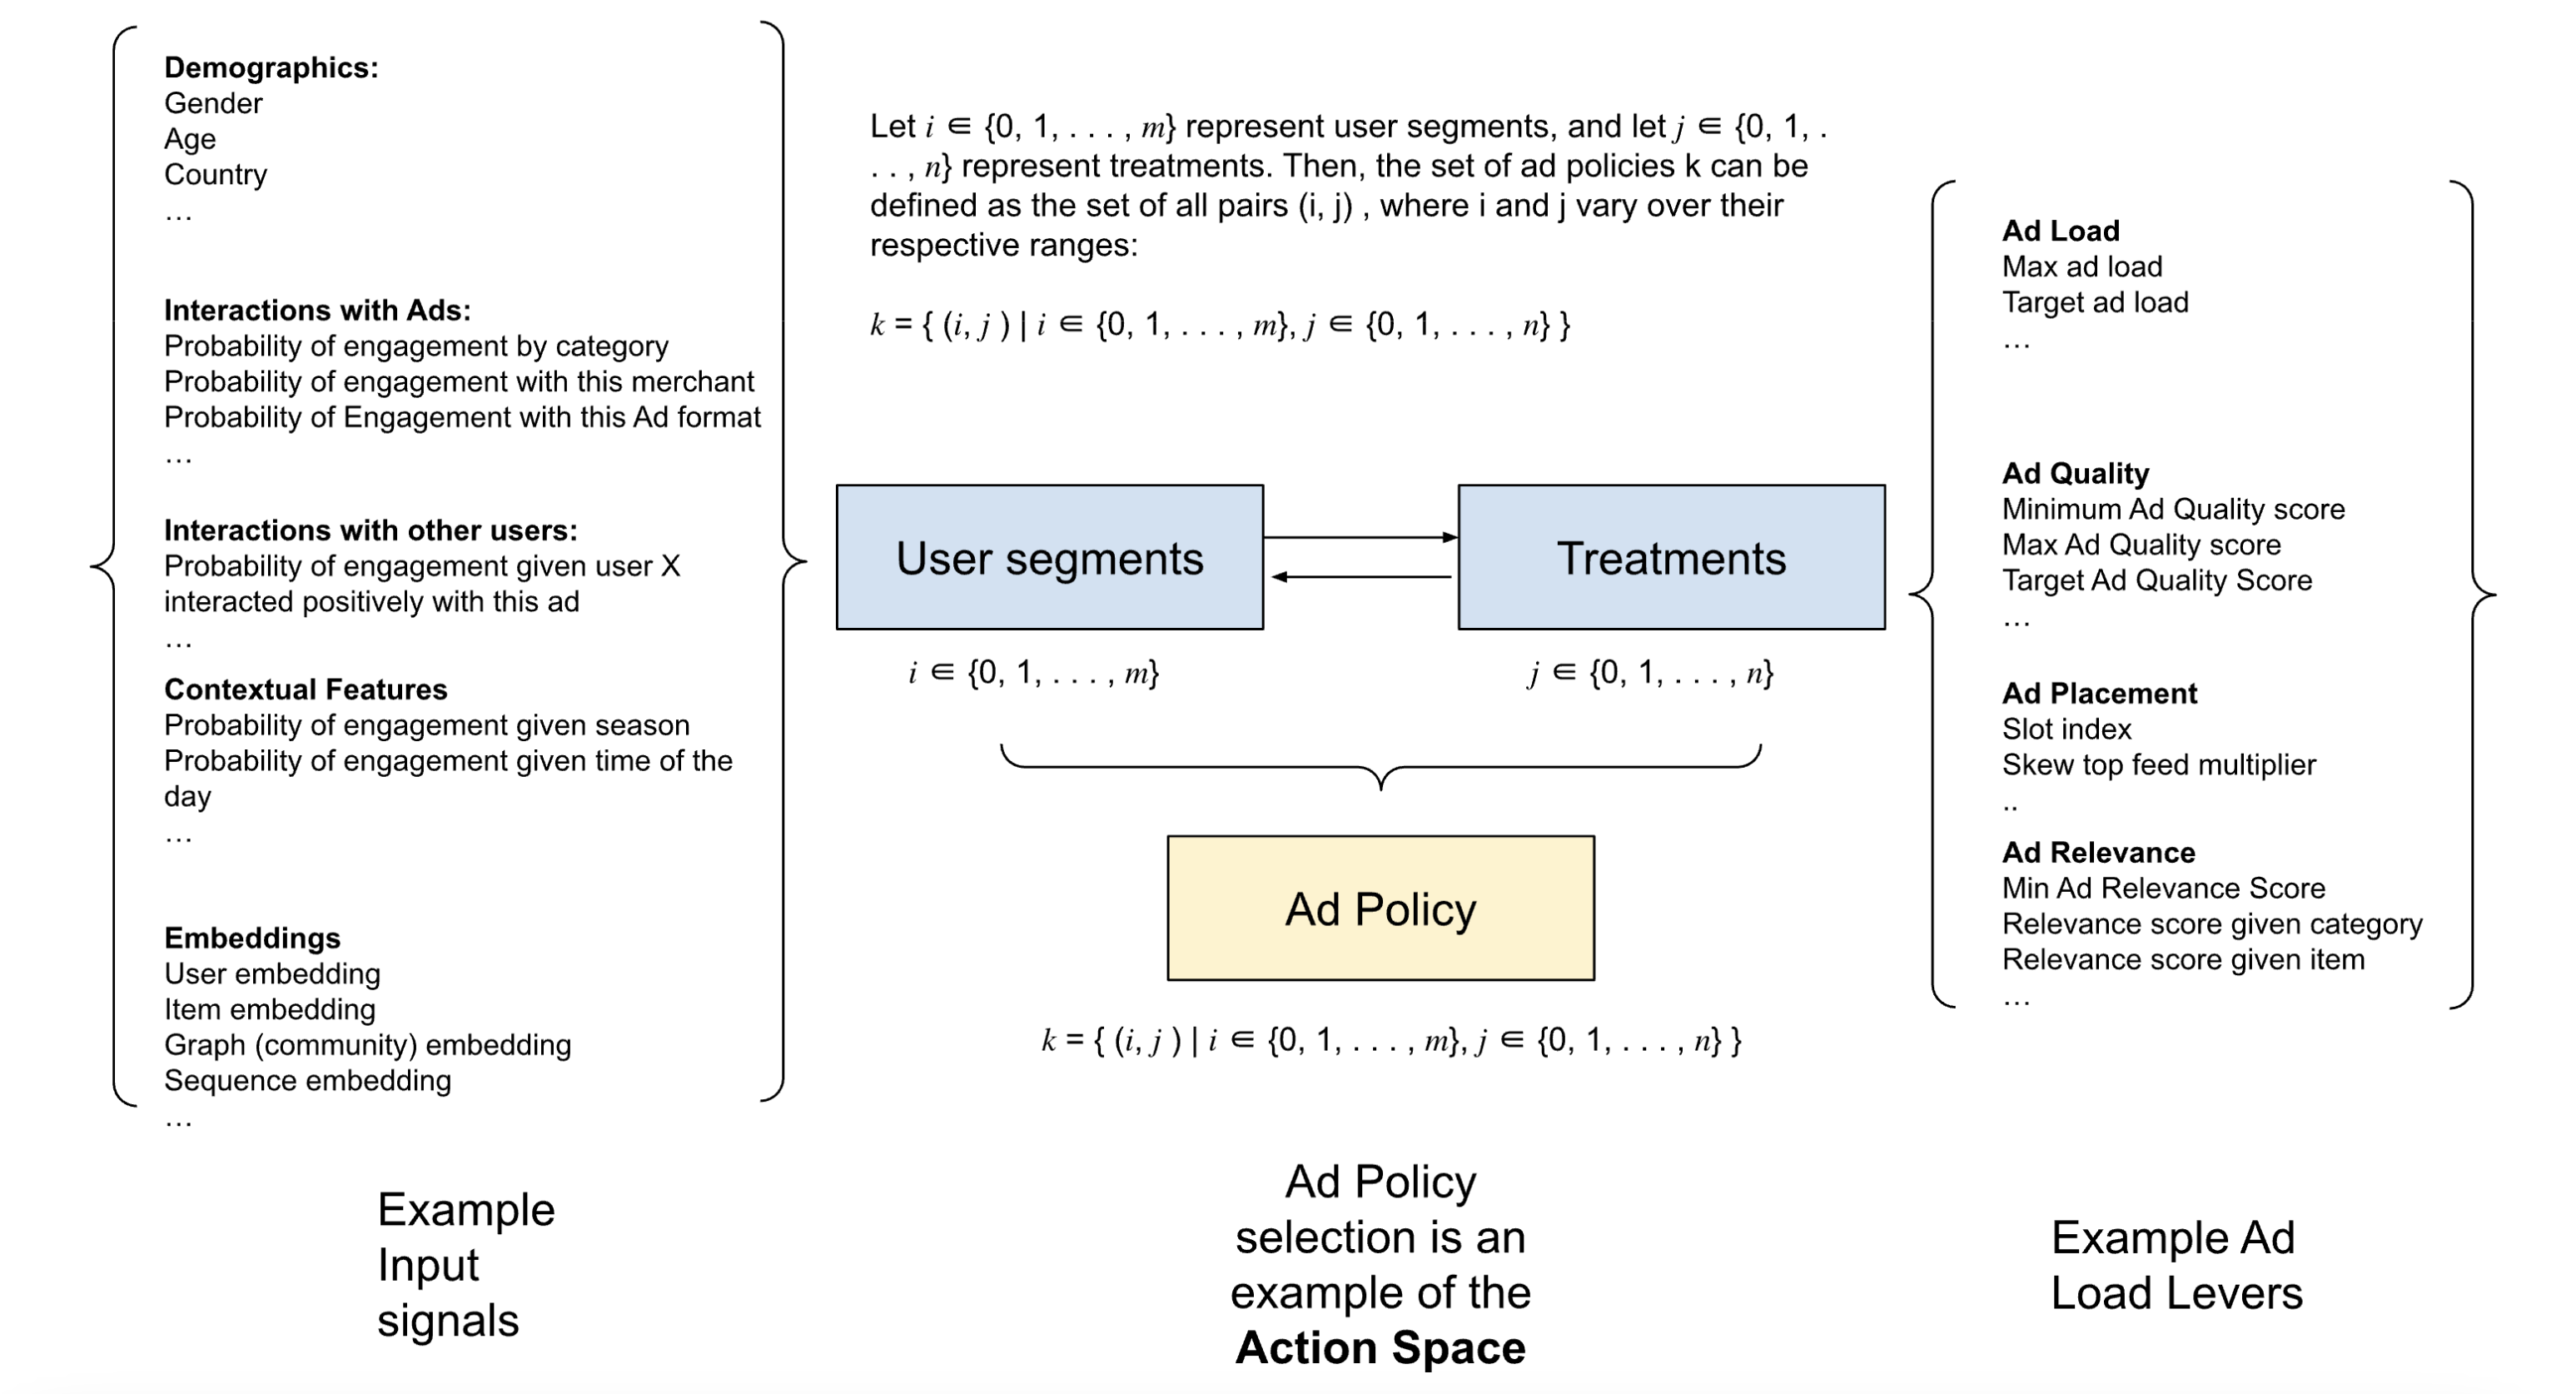
\includegraphics[width=\textwidth]{detailed_ad_policy.png}
    \caption{Example of an action set in the context of ad policies in recommendation systems}
    \label{fig:detailed_ad_policy}
\end{figure*}

\section{Conclusions}

The integration of RL in policy optimization for large-scale recommender systems has gained popularity as a promising approach to balance long-term and short-term objectives in environments with complex user behavior and revenue dynamics. However, scaling RL in practice presents challenges, including vast state and action spaces, reliance on proxy metrics, and significant computational demands. This paper provides an overview of effective, scalable techniques that address these challenges, offering insights into how RL can be applied at scale.
Unlike traditional methods that focus on optimizing short-term outcomes, RL’s cumulative reward framework enables it to account for both immediate and delayed feedback. Together, contextual bandits and offline replay offer scalable, interpretable solutions that approximate full RL while managing real-time constraints. Contextual bandits support selecting optimal actions within each interaction based on the current state, maximizing immediate rewards, which are typically proxy metrics of the true long-term reward. Offline replay complements this by enabling counterfactual learning: multiple treatments can be tested across randomized populations to evaluate causal effects, refining policies for diverse user segments.

Future research may focus on enhancing interpretability, refining reward functions, and exploring decentralized approaches to handle complex decision layers. These advancements will bring RL closer to fulfilling its potential in providing tailored, dynamic ad recommendations that align user satisfaction with business goals in large-scale recommendation systems.




\section*{Acknowledgements}
I would like to thank my advisor, Yuri Lawryshyn, for his valuable guidance and direction throughout this work. I also extend my gratitude to Adam Obeng, Bee-Chung Chen, and Jay Adams for their critical coaching and insights, which have significantly shaped my approach and understanding of industry practices. Their expertise has been key in aligning academic research with practical applications.

% This unnumbered section should be blank when submitting your paper. After review, you may include lists of people and organizations who supported the work.

% Print the biblography at the end. Keep this line after the main text of your paper, and before an appendix. 
% % THIS IS A LATEX TEMPLATE FILE FOR PAPERS INCLUDED IN THE
% *Anthology of Computers and the Humanities*. ADD THE OPTION
% 'final' WHEN CREATING THE FINAL VERSION OF THE PAPER. 
% DO NOT change the documentclass
%\documentclass[final]{anthology-ch} % for the final version
\documentclass[final]{anthology-ch}         % for the submission

% LOAD LaTeX PACKAGES
\usepackage{booktabs}
\usepackage{graphicx}
\usepackage{tabularx}
\usepackage{adjustbox}  % lets us make the table wider than \textwidth
\usepackage{setspace}
\usepackage{enumitem}
\usepackage{makecell}
% \usepackage{multirow}
\usepackage{float}

% \usepackage[table,xcdraw]{xcolor} % Allows the use of HTML colors

\addbibresource{bibliography.bib}


% \PassOptionsToPackage{table,xcdraw}{xcolor}


\geometry{
  a4paper,
  top=2cm,
  bottom=2cm,
  left=2cm,
  right=2cm
}

% ADD your own packages using \usepackage{}

% TITLE OF THE SUBMISSION
% Change this to the name of your submission
\title{A Review of Reinforcement Learning Applications in Ad Policy Optimization for Large-Scale Recommender Systems}

% AUTHOR AND AFFILIATION INFORMATION
% For each author, include a new call to the \author command, with
% the numbers in brackets indicating the associated affiliations 
% (next section) and ORCID-ID for each author.  
\author{Armando Ordorica}

\author{Yuri Lawryshyn}

% While we encourage including ORCID-IDs for all authors, you can
% include authors that do not have one by definining an empty ID.


% There should be one call to \affiliation for each affiliation of
% the authors. Multiple affiliations can be given to each author
% and an affiliation can be given to multiple authors. 
\affiliation{University of Toronto, Toronto, Canada}

% KEYWORDS
% Provide one or more keywords or key phrases seperated by commas
% using the following command

\keywords{Reinforcement Learning, Ad Policy Optimization, Contextual Bandits, Recommendation Systems,  Off-Policy Learning, Online Advertising, Deep Reinforcement Learning,  Multi-Objective Optimization}

% METADATA FOR THE PUBLICATION
% This will be filled in when the document is published; the values can
% be kept as their defaults when the file is submitted
\pubyear{2025}
\pubvolume{1}
\pagestart{1}
\pageend{1}
\conferencename{Proceedings of Conference XXX}
\conferenceeditors{Editor1 Editor2}
\doi{00000/00000}  

% \addbibresource{bibliography.bib}


\setstretch{2.0}

\begin{document}


\maketitle
% \doublespacing

\begin{abstract}
Balancing advertisements with organic content in large-scale recommendation engines is a well-known challenge in the industry. While ads are essential for revenue generation in platforms that integrate them alongside organic content, they often underperform in user engagement compared to organic content \cite{hochstein2023toward}. The key challenges in achieving this balance include ad selection, ranking, and integration with organic content. These involve decisions about whether to insert an ad, which ad to select, and where to place it \cite{zhao2020jointly}. Traditional methods optimize for the highest probability of ad clickthrough with fixed placements and are typically solved as supervised Machine Learning (ML) problems \cite{covington2016deep}. However, these approaches focus on optimizing single actions, overlooking the downstream impact of sequential user behavior and underutilizing valuable contextual signals. A more dynamic approach that accounts for context and optimizes the long-term value of action sequences, balancing both engagement and revenue, remains an open research area \cite{lin2023survey}.\\

Reinforcement Learning (RL) offers a promising framework to address the need for dynamic, context-aware optimization by formalizing the process of finding the best policy in sequential decision-making under uncertainty \cite{dimitrakakis2018decision}. However, implementing RL in large-scale recommendation systems faces challenges such as vast state and action spaces, the risk of poorly chosen reward functions, high computational costs \cite{pancha2022pinnerformer}, and the difficulty of interpreting online policy learning \cite{van2024practical}. This paper surveys existing methodologies and frameworks that utilize RL to enhance recommendation strategies, aiming to guide practitioners and researchers in navigating these challenges. Our analysis reveals that while fully online RL is powerful in theory, in practice, techniques like contextual bandits, offline replay, and surrogate reward modeling often yield more scalable and interpretable solutions for large-scale ad-serving.
\end{abstract}

% \tableofcontents

\section{Introduction}

Platforms such as Google, Meta, TikTok, and Pinterest offer content recommendation systems whose revenue models depend on an effective balance between advertisements and organic content \cite{zhao2020jointly} \cite{danescu2010competing}. This balance is essential to maximize immediate revenue while avoiding long-term issues such as ad fatigue, where users become less responsive to ads due to overexposure, and user churn, where users discontinue using the platform \cite{sagtani2023quantifying} \cite{silberstein2023combating}.\\

Over the past decade, deep learning has emerged as a promising technique that enables recommendation engines to better understand context through embeddings, significantly improving their ability to personalize content \cite{naumov2019deep} \cite{zhao2024survey}. However, deep learning approaches are often supervised and rely on measurable and observable short-term metrics used as model labels, such as the probability of a click-through or the likelihood of a video being watched in full \cite{nvidia_recommender_systems_2021}. Methodologies that use myopic objective functions to optimize these directly measurable short-term metrics often overlook the long-term value of a recommendation \cite{mazoure2021improving}. By focusing on immediate rewards, they may rank content based on short-term engagement metrics while neglecting the entire sequence of user interactions that involve delayed responses. Such approaches can result in suboptimal outcomes, such as promoting clickbait content that compromises long-term revenue and user engagement.\\

	% 4.	How does Reinforcement Learning (RL) offer a promising solution to these challenges?

To overcome the challenges of optimizing based solely on immediate objectives, Reinforcement Learning (RL), modeled as a Markov Decision Process (MDP), has emerged as a promising framework \cite{afsar2022reinforcement}. RL enables the consideration of long-term value by optimizing policies that maximize cumulative rewards over time, rather than focusing on short-term engagement metrics. In an MDP, actions are selected based on a policy ($\pi$), which chooses the action that maximizes the expected cumulative reward from the current state onward. This cumulative reward is typically conceptualized as the expected sum of future rewards, discounted over time using a discount factor. A lower discount factor places more emphasis on immediate rewards, effectively ignoring future outcomes. Conversely, a discount factor approaching one values future rewards more heavily, encouraging the policy to consider long-term benefits \cite{Sutton1998}. \\

In the context of recommendation systems, rewards can be defined to capture both user engagement and revenue objectives. Engagement rewards might include metrics such as time spent on the platform, content views, clicks, saves, shares, or likes \cite{wang2022surrogate}. Revenue rewards can be tied to ad-related metrics like ad impressions, ad clicks, conversions, or purchases resulting from ad exposure. These different rewards are often combined into a single utility function that reflects the platform’s overall objectives \cite{zhao2020jointly} \cite{zou2019reinforcement} \cite{xu2023optimizing}.\\

For example, the reward function  $r_t$  at time  $t$  can be defined as:

$$
r_t = \alpha \times \text{Engagement Metric}_t + \beta \times \text{Revenue Metric}_t,
$$ where  $\alpha$  and  $\beta$  are weighting factors that balance the importance of user engagement and monetization. By appropriately defining the utility function and choosing suitable weights, RL algorithms can optimize policies that enhance user experience while maximizing revenue over the long term \cite{zhao2020jointly, zhao2021dear, yan2020ads, sagtani2024ad}. \\


% What specific challenges are encountered when implementing RL in large-scale recommendation systems?
Despite the promising theoretical framework that RL offers for optimizing long-term value in recommendation systems, implementing RL in real-world, large-scale platforms remains complex \cite{dulac2021challenges}. First, in the context of recommendation systems, the state space, which reflects the current context of the user and the environment, and the action space, which captures how the recommender system can be tuned, are both essentially infinite \cite{zhu2021overview}. This vastness makes learning and optimization computationally intensive and difficult to discretize into individual actions and states, a critical requirement for policy learning \cite{afsar2022reinforcement} . \\ 

Second, designing appropriate reward functions is critical, as poorly chosen reward functions can lead to unintended system behaviors that degrade user experience or negatively affect business revenue \cite{everitt2021reward}. For example, a reward function that overly prioritizes click-based metrics may drive the system to promote clickbait content, boosting short-term engagement but eroding user trust and satisfaction over time \cite{wu2017returning}. Similarly, a reward function too heavily skewed toward revenue metrics could result in excessive ad load, disrupting the user experience and leading to churn. Striking the right balance in reward function design is essential to achieve both user engagement and monetization objectives without compromising the platform’s long-term goals.\\


Furthermore, interpretability is a major challenge in RL deployment. Understanding the learned policies--the strategies adopted by the RL agent--can be particularly difficult when policies are updated in real-time during user interactions (online policy learning) \cite{glanois2024survey} \cite{vouros2022explainable} \cite{dulac2019challenges}. This real-time adaptation complicates monitoring and evaluation, making it challenging to understand what is happening during online learning. In extreme cases, this lack of transparency could result in non-compliant or unethical behavior, posing significant risks to both users and the business \cite{lambert2023entangled}.\\

	% 7.	What are the objectives and contributions of this paper?
In light of the challenges outlined above, this paper examines methodologies and frameworks used to implement RL for large-scale recommendation systems, with a particular focus on contexts where ad revenue is central to the business model. Although previous surveys address RL in recommendation systems \cite{lin2023survey, afsar2022reinforcement}, they do not specifically explore how RL can balance the competing demands of ad and organic content. This paper fills that gap by analyzing approaches tailored to these unique challenges and bridging the divide between theoretical RL concepts and their real-world applications.
\\

The paper begins with a historical overview of ad selection and ranking systems, tracing the evolution from simple rule-based models and heuristic approaches to tree-based models and modern deep learning techniques. Each of these stages is explored in detail, highlighting their limitations and the motivations for adopting RL as the next paradigm in recommendation systems. Following this contextual history and motivation, the paper introduces key RL components such as the action space, state space, reward functions, and policies, using a straightforward toy example: the frozen lake problem. This example provides a foundation for understanding RL fundamentals, which are then mapped to real-world challenges in online advertising and recommendation systems. Drawing on these analogies, the paper offers a clear and practical framework to help practitioners navigate the implementation of RL and adapt these methodologies to their specific needs.


	% 8.	How will this paper help practitioners and researchers navigate the challenges of implementing RL in recommendation systems?


	% 13.	What is the structure of the paper, and what can readers expect in the subsequent sections?

\section{Paper Collection Methodology}

To ensure broad coverage, relevant papers were collected from both academic and industry sources. Foundational academic works such as \textit{Reinforcement Learning: An Introduction} \cite{Sutton1998}, \textit{Statistical Methods for Recommender Systems} \cite{agarwal2016statistical}, and \textit{Artificial Intelligence: A Modern Approach} \cite{russell2016artificial} were used to establish key mathematical foundations, including Markov Decision Processes (MDPs), Contextual Bandits, Off-Policy Learning, and Offline Replay.

To reflect the internal perspective of a production-facing ad policy team, a curated list of 10–15 papers referenced within Pinterest’s Ad Policy team was also compiled. Examples include \textit{Jointly Learning to Recommend and Advertise} \cite{zhao2020jointly}, \textit{DEAR: Deep Reinforcement Learning for Online Advertising Impressions in Recommender Systems} \cite{zhao2021dear}, \textit{Ad-load Balancing via Off-Policy Learning} \cite{sagtani2024ad}, and \textit{Practical Bandits} \cite{van2024practical}. In addition, targeted keyword searches such as “Reinforcement Learning ads [company name]” and “Contextual Bandit [company name]” were conducted for leading companies in the advertising and recommendation space (e.g., Google, Meta, Pinterest, Microsoft, TikTok, YouTube, LinkedIn),  surfacing additional papers describing real-world systems and methodologies. To complement those efforts, a separate search was conducted on Google Scholar for relevant review papers. While no surveys were found that specifically focused on RL in ad recommendation systems, related reviews on "contextual bandits", "ad fatigue", and "recommender systems" were used to identify additional references.

Finally, manual crawling of citation networks in cornerstone papers was used to identify additional key contributions. For instance, tracing citations from \textit{Jointly Learning to Recommend and Advertise} \cite{zhao2020jointly}, \textit{DEAR} \cite{zhao2021dear}, and \textit{Offline Reinforcement Learning} \cite{levine2020offline} led to works such as \textit{Ads Allocation in Feed via Constrained Optimization} \cite{yan2020ads} and \textit{A Contextual Bandit Bake-off} \cite{bietti2021contextual}.
In total, 153 papers were selected and reviewed. Papers were ranked according to three main criteria: influence, to capture the foundational or widely adopted ideas in the field; industry relevance, to ensure that the outcomes were sound, implementable, and actionable; and recency, to reflect the latest methodological developments and deployment practices.

While recent and highly cited work was prioritized, papers introducing novel methodologies were also included regardless of citation count. To contextualize the selected works, this survey builds from the ground up. Each component of the Markov Decision Process, including states, actions, rewards, and policies, is defined and illustrated using a toy example such as the Frozen Lake. This foundation is then extended to practice through a review of how each component is operationalized in industry, along with a discussion of the limitations of those approaches. Drawing on existing methods and lessons from industry, the resulting framework is intended to inform practitioners exploring how RL can be applied in their organizations to develop ad policies that balance monetization with organic engagement. A comparison between the toy example and real-world implementation parallels can be found in Table \ref{tab:comparison}.



\section{A Brief History of Ad Selection and Ranking in Recommendation Systems}

\begin{figure}[ht]
    \centering
    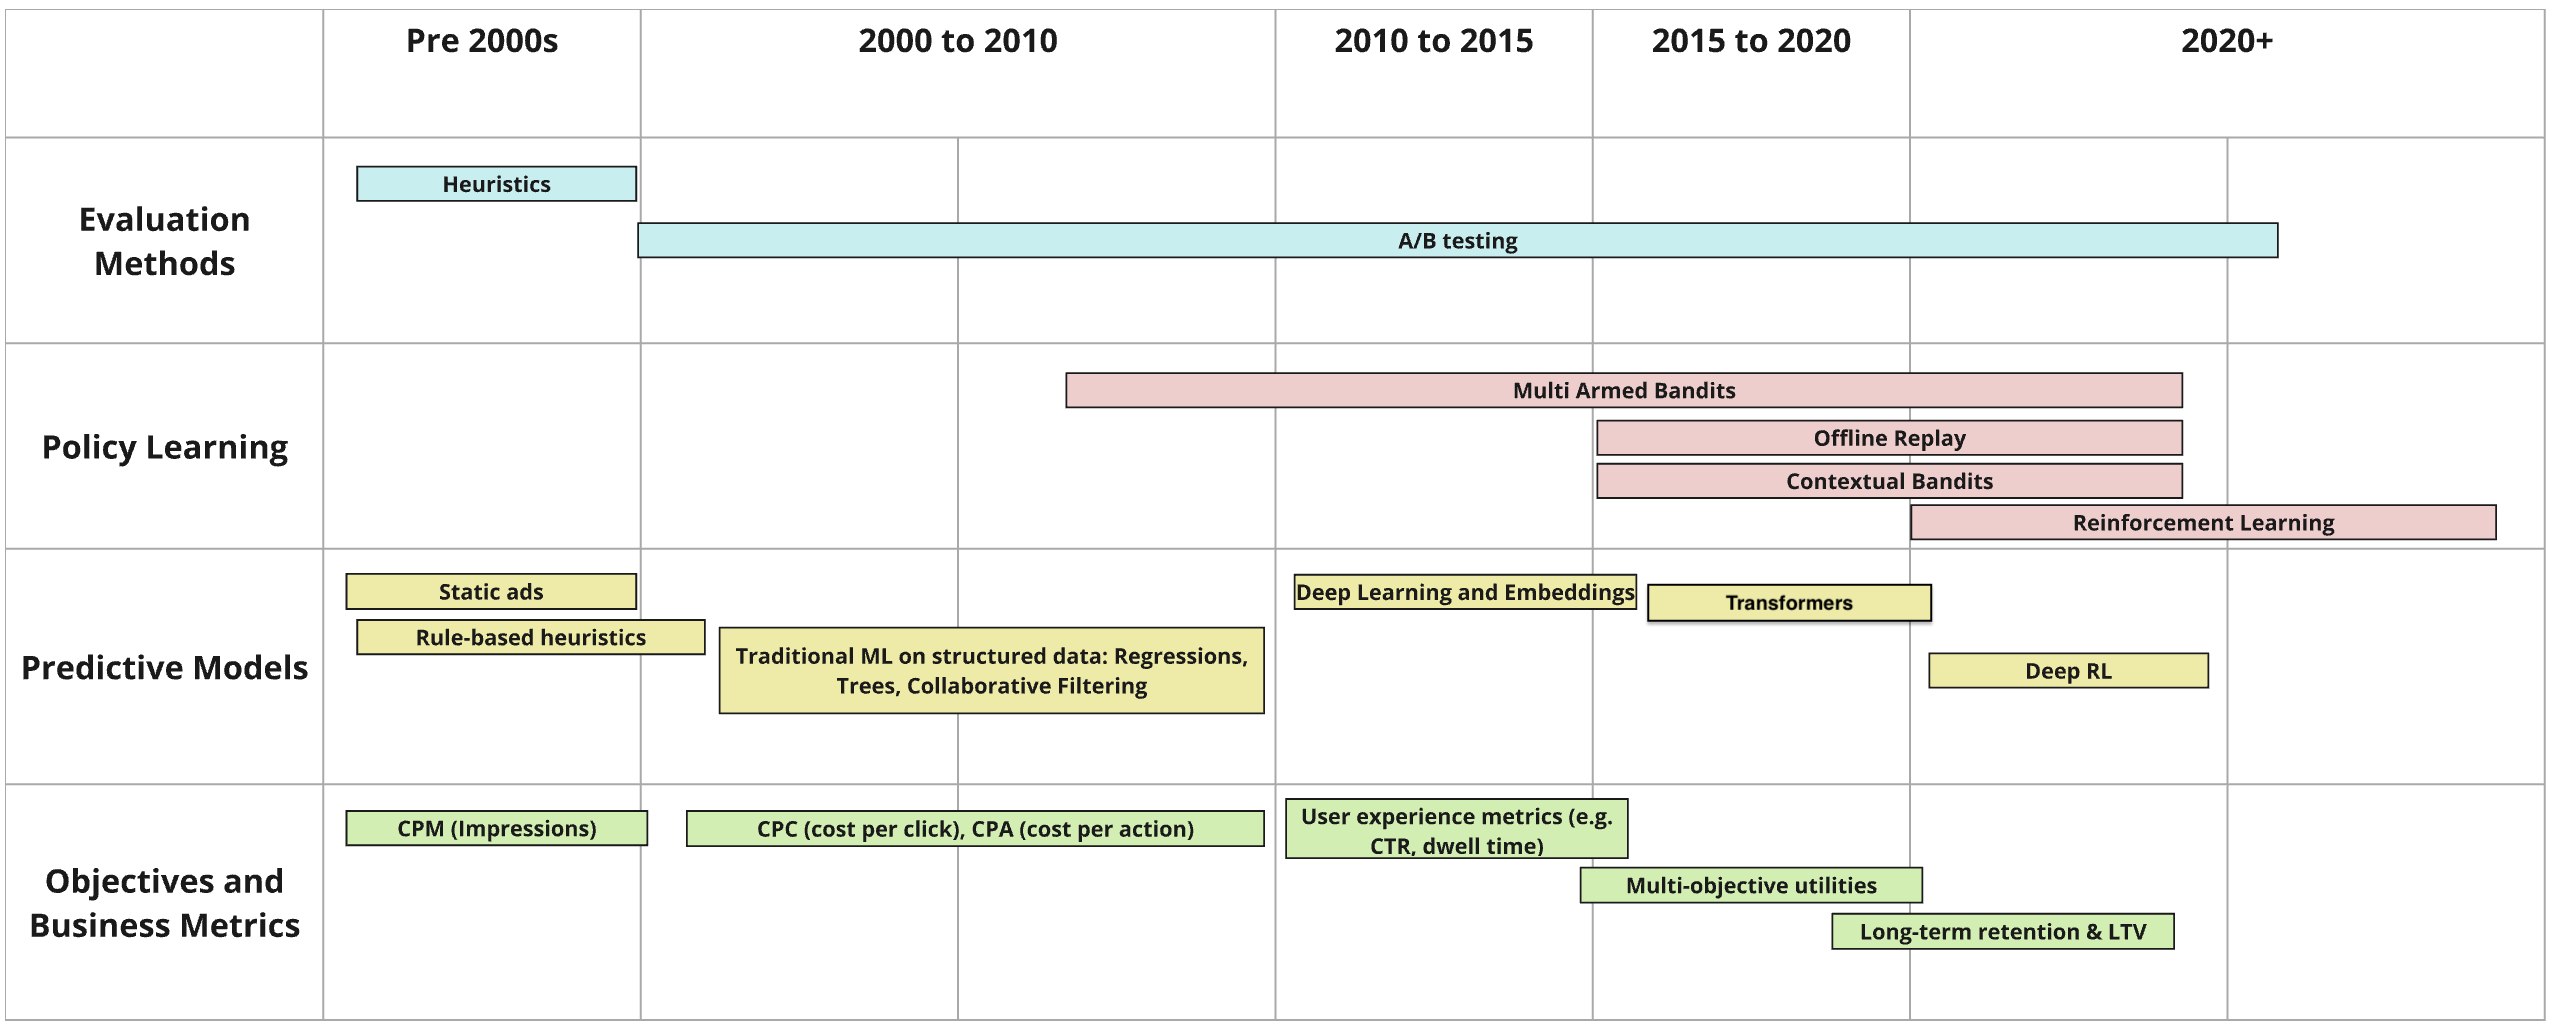
\includegraphics[width=\textwidth]{history_timeline_figure.png}
    \caption{Timeline Showing Initial Adoption and Popularization of Techniques and Methodologies in Online Advertising}
    \label{fig:ad_timeline}
    \vspace{0.2cm} % adds small vertical spacing
    \begin{flushleft}
        \footnotesize{\textit{Note:} The boundaries and lengths of rectangles are approximate. Innovations and transitions between techniques and objectives occurred gradually and continuously, rather than sharply at specific dates.}
    \end{flushleft}
\end{figure}


In online advertising, a good ad policy can result in positive revenue for the company while also boosting user experience. Conversely, a poor ad policy involves showing ads that are irrelevant to the user’s current intent, overloading the feed with excessive ad density, and failing to align content with the user’s interests. Irrelevant ad targeting can lead to ad fatigue, a state where users become desensitized or frustrated by excessive or poorly targeted ads, resulting in decreased engagement with both the ads and the platform as a whole \cite{ccelik2023ad}. \\

This section traces the evolution of advertising recommendation algorithms, culminating in the adoption of RL to overcome the limitations of earlier approaches. It begins by outlining how early online advertising primarily mirrored offline methods through banner ads and other static formats. It continues by explaining how static online advertising evolved over time to incorporate rule-based models and more sophisticated heuristic techniques. The discussion then transitions to the integration of machine learning methods, including regression-based models, tree-based algorithms, and collaborative filtering, followed by the emergence of deep learning and embedding-based approaches that effectively capture the nonlinear interactions between users and content. Finally, RL is introduced as a promising solution to address the shortcomings of preceding methodologies. This evolution is visually represented in Table \ref{fig:ad_timeline}, which shows the initial adoption and popularization of techniques and methodologies in online advertising. \\

\subsection{From Rule-Based Advertising to Traditional Machine Learning}
\textbf{Around the early 2000s, online advertising largely mirrored offline practices, heavily relying on non-targeted formats such as banner ads \cite{kant2021history}.} These generic advertising methods conflicted with the objective of search engines of efficiently directing users to relevant content \cite{fain2006sponsored}. As a marginal improvement on nontargeted ad formats like banner ads, advertisers began to utilize simple \texttt{if-then} logic with predefined rules to select and display ads based on basic criteria like user demographics. While rule-based systems were straightforward to implement, their lack of flexibility and personalization became evident as ad fatigue, defined as reduced user engagement due to repeated exposure to the same advertisement, persisted \cite{abrams2007personalized}. This issue underscored the necessity of not only leveraging user signals but also optimizing ad load tuning parameters, such as frequency and placement, to maintain user interest and maximize click-through rates \cite{abrams2007personalized}. For instance, researchers at LinkedIn introduced concepts like top slot - highest eligible position for an ad within the feed -  and minimum gap - the required distance between consecutive ads to prevent oversaturation - as ad load tuning parameters \cite{yan2020ads}. Their research indicated that users are more likely to click on ads that are spaced farther apart \cite{yan2020ads}. \\

\textbf{The evolution of ad pricing, from paying for impressions to paying for user actions, created pressure within the online advertising industry to improve relevance and performance-based metrics \cite{hu2004performance}.} Sponsored search, introduced by GoTo (later Overture), allowed advertisers to bid on specific keywords, directly linking ads to user queries and addressing the limitations of generic advertising  \cite{fain2006sponsored}. Foundational pricing models, such as Cost per Mille (CPM), charged advertisers per 1,000 impressions and closely mirrored offline practices \cite{wikipedia-cpm}. Yahoo!, through the acquisition of Overture \cite{wsj2003yahoooverture}, later introduced Cost per Click (CPC) \cite{ellam2003overture}, a performance-based pricing model that shifted costs to reflect measurable user engagement. This evolution continued with the introduction of Cost per Action (CPA), which tied fees to specific user actions beyond clicks, such as purchases or sign-ups. These changes incentivized the advertising industry to innovate, leading to the development of more relevance-focused strategies. These foundational pricing models remain integral to the utility functions that underpin contemporary ranking algorithms \cite{fain2006sponsored}. As advertisers increasingly demanded performance-based pricing, the ad tech industry was compelled to innovate within a competitive yet lucrative market, addressing the limitations of rule-based and heuristic models through the adoption of machine learning techniques to enable more dynamic and data-driven approaches \cite{zhang2018whole}.



\textbf{The next set of innovations following heuristics and performance-based targeting was led by machine learning (ML) and A/B testing \cite{barajas2022online}}. From 2010 to 2015, ad selection techniques evolved significantly with the adoption of machine learning models such as Logistic Regression, Decision Trees, and Gradient Boosting Machines \cite{cui2015global}. By leveraging historical data and diverse user behavior signals, these models enabled more accurate predictions of user engagement \cite{cui2015global}. In parallel, A/B testing allowed practitioners to systematically compare models and features, ensuring that any new implementation delivered measurable performance gains \cite{barajas2022online}.
Despite these successes, traditional tabular models struggled to capture nuanced user intent, particularly when processing more complex data such as images or text. In the early 2010s, deep learning gained momentum with breakthroughs like AlexNet \cite{krizhevsky2012imagenet}, which demonstrated the power of neural networks to handle unstructured high-dimensional data. This ability to capture complex, nonlinear interactions dramatically improved ad recommendations, especially through the use of embeddings, which are dense vector representations that map words or images into high-dimensional spaces. Metrics like cosine similarity further refined personalization by aligning recommendations with user interests \cite{covington2016deep}. Embedding-based models, particularly two-tower architectures, presented a major leap forward in ad recommendation systems by effectively capturing intricate relationships between users and ads. These models utilize two neural networks: one dedicated to encoding user information and the other to encoding ad (item) information. The outputs from these networks are then combined to predict user engagement with ads \cite{vorotilov2023scaling}. This approach not only boosted accuracy but also scaled effectively. Despite the significant improvements that embedding-based models introduced in terms of predictive accuracy and scalability of ad recommendation systems, the practical challenges of balancing multiple objectives, such as maximizing revenue, mitigating ad fatigue, and sustaining long-term user engagement remained unresolved.  


\textbf{Multi-Armed Bandits (MABs) emerged as a powerful method for online advertising around the 2010s to minimize user exposure to suboptimal ad configurations, effectively tackling the explore–exploit tradeoff, which consists of finding the optimal balance between choosing new ad policies with unknown performance and showing older ad policies with known positive performance \cite{schwartz2017customer} \cite{burtini2015improving}.} MABs are a class of algorithms for dynamic decision-making under uncertainty, originally developed in mid-20th-century probability theory \cite{robbins1952sequential}. While MABs had been widely applied in areas such as clinical trials \cite{villar2015multi} \cite{thompson1933likelihood}, they only gained significant traction in online advertising around the 2010s \cite{schwartz2017customer}.  

MABs allow platforms to reduce unnecessary exposure to a suboptimal treatment by continuously updating the probability distribution of which treatment is most likely to yield the highest reward \cite{kuleshov2014algorithms}. In clinical trials, for instance, a bandit algorithm reduces unnecessary exposure to suboptimal treatments by updating its reward estimates in real time: it allocates more patients to the better-performing treatment (exploitation) while still testing others that could be better (exploration) \cite{kuleshov2014algorithms}\cite{villar2015multi}. In this setting, the “reward” might be a measurable improvement in patient health or recovery time \cite{villar2015multi}. The same principle applies to online advertising, where “treatments” translate into specific ad configurations, defined by parameters such as displacement cost, reserve price, ad load, and ad placement. “Rewards” in online advertising typically represent user engagement metrics such as clicks or conversions \cite{schwartz2017customer}. Advertising platforms should continuously “explore” new treatments to test new ads, formats, and targeting strategies to avoid stagnation, while simultaneously “exploit” existing high-performing treatments to ensure near-term revenue targets are met \cite{schwartz2017customer}.  

In contrast to traditional A/B tests, where there are randomized treatments assigned for a predetermined amount of time, MABs dynamically learn which configuration yields the highest reward for each user at a particular time. This approach reduces the time users are exposed to suboptimal ad configurations, thereby mitigating losses in engagement and long-term revenue \cite{schwartz2017customer}. Although this dynamic learning framework effectively tackles the explore–exploit tradeoff, defining the precise set of rewards and objectives to optimize remains an open challenge, particularly when advertisers must juggle multiple goals such as revenue and long-term user satisfaction \cite{wen2019learning}.

\textbf{To address this need for clear, multi-objective definitions, such as balancing user satisfaction and revenue, utility functions have been employed in online advertising since the early 2000s \cite{engel2008incorporating}.} Rooted in microeconomic theory dating back to the mid-20th century, utility functions are mathematical constructs that quantify preferences and the net value of conflicting objectives \cite{Stigler1950} \cite{vonNeumannMorgenstern1944}. Introduced to formalize decision-making under uncertainty, they model and quantify consumer preferences, enabling advertisers and publishers to encode multiple objectives, such as revenue, user satisfaction, and long-term platform health, into a single or composite utility metric \cite{engel2008incorporating}. By integrating utility functions into MAB-based frameworks, advertisers can systematically guide the exploration–exploitation process toward a unified reward signal that balances short-term performance (e.g., clicks, impressions, or conversions) with long-term considerations (e.g., minimizing ad fatigue or maintaining user trust). This approach allows for principled trade-offs, optimizing for immediate gains while safeguarding long-term engagement.


\subsection{Advances in Deep Learning: Attention Models, Transformers, and Contextual Bandits}

\textbf{While embedding-based models greatly enhanced the predictive power of recommendation systems, capturing the full complexity of user sequences, especially over long time spans, remained a challenge for sequential deep learning methods such as  Long Short-Term Memory networks (LSTMs) and Gated Recurrent Units (GRUs) \cite{vaswani2017attention} \cite{gao2024mamba}.} Traditional recurrent networks (e.g., LSTMs or GRUs) process sequences step by step, typically encoding an entire sequence into a single fixed-size vector \cite{Sutskever2014}. This design poses several challenges. Because Recurrent Neural Networks (RNNs) operate strictly in a sequential manner, they cannot process multiple parts of the sequence in parallel, creating bottlenecks and risking the loss or blurring of details, especially those from earlier steps in long sequences \cite{vaswani2017attention}.  Moreover, standard RNNs inherently prioritize recent inputs as information is passed along, which attenuates earlier signals and leads to the well-known vanishing gradient problem in lengthy sequences and fails to effectively capture long-term dependencies \cite{Bengio1994}\cite{Pascanu2013}. 


\textbf{To address training inefficiencies in RNNs and the difficulty of capturing long-term dependencies, attention mechanisms allow direct access to any position in the sequence, enabling the model to focus on relevant features in the sequence regardless of their temporal distance \cite{vaswani2017attention}. }By computing pairwise interactions across all positions in the sequence, Transformers overcome the sequential bottlenecks of RNNs and enable parallel computation \cite{vaswani2017attention}.  This mechanism also allows the model to incorporate contextual signals, such as user demographics, session-level metadata, or item attributes, at any point in the sequence, rather than strictly depending on a running hidden state \cite{kang2018sasrec}. The ability to attend to any part of the input at any time allows Transformers to model long-range dependencies with far greater efficiency and accuracy than RNN-based architectures \cite{vaswani2017attention}. This paradigm shift led to the development of the Transformer architecture, which entirely replaces recurrence with self-attention, fundamentally redefining sequence modeling \cite{vaswani2017attention}.

\textbf{The Transformer’s parallel attention architecture is a natural fit for modern hardware.} Since self-attention and feed-forward layers are implemented with large matrix operations, the model makes efficient use of Graphics Processing Units (GPUs) and Tensor Processing Units (TPUs), which excel at parallel computation \cite{vaswani2017attention}. Unlike RNNs that left many GPU cores underutilized due to their step-by-step nature, Transformers keep the hardware busy by processing many elements concurrently. This yields significantly shorter training times compared to earlier recurrent models. Moreover, Transformers scale up seamlessly: training can be distributed across multiple GPUs, and larger batches or longer sequences can be handled without a drop in throughput \cite{shim2022comparison}. Engineers can simply add more GPU workers to accommodate bigger models or more data, achieving near-linear speedups in many cases \cite{brown2020language}. The ability to train deep models efficiently at scale has unlocked previously impractical projects, and Transformer-based architectures (e.g. BERT, GPT) are now standard building blocks in modern AI systems \cite{brown2020language} \cite{kaplan2020scaling}. One of the key innovations of the Transformer architecture is its multi-head attention mechanism \cite{vaswani2017attention}. Instead of relying on a single attention distribution, multiple attention “heads” are trained in parallel, each with its own set of learned parameters. This design allows the model to capture a range of relationships or patterns within the same sequence \cite{vaswani2017attention}.In practice, each head can focus on different aspects. One head might emphasize local dependencies in the user’s interaction history, while another one might highlight more global, long-range correlations \cite{vaswani2017attention}.


\textbf{In an advertising context, multi-head attention naturally accommodates multi-objective learning \cite{ma2018modeling}.} For example, one head could be tuned to prioritize short-term engagement metrics (e.g., click-through rate or CTR) by attending to recent user activities and relevant ad features, while another head could emphasize longer-term outcomes, such as mitigating ad fatigue or preserving user satisfaction \cite{zhao2019recommending} \cite{ma2018modeling}. Each head learns a distinct set of attention weights, enabling the model to isolate and capture unique signals that serve different goals \cite{an2024tmh}. The outputs from these multiple heads are then aggregated, typically concatenated and linearly transformed, into a single representation or score, providing a unified but multi-faceted embedding of user–ad interactions \cite{vaswani2017attention} \cite{lyu2023entire}. However, determining the appropriate attention heads and their optimal weighting remains a complex challenge \cite{vaswani2017attention}\cite{Kang2018} \cite{Voita2019}. The optimal weights may vary not only across different users and content types but also over time \cite{Zhou2018} \cite{Zhou2019}. Additionally, shifting business objectives, engineering constraints, and competing optimization objectives further complicate the design process \cite{Mehrotra2018} \cite{Mehrotra2020} \cite{Jannach2023}. 

%How is head selection and weighing typically done 
\textbf{Selecting the right heads in Multi-Task Attention Models and determining their optimal weighting is not a deterministic process \cite{Michel2019} \cite{Voita2019}.} It typically requires iterative experimentation, involving both offline analysis (e.g., hyperparameter tuning, head ablation studies) and online testing (A/B experiments) \cite{Michel2019} \cite{kang2018sasrec}. This process is particularly challenging for new users and new content, where slow adaptation can result in suboptimal personalization and early churn \cite{Schein2002, Bobadilla2013}. 

%tie this up to Offline Replay 
\textbf{To address difficulties related to policy optimization - like weight tuning and head selection - \textit{Offline Replay} is often employed to find optimal policies in large parameter search spaces  \cite{agarwal2016statistical} \cite{levine2020offline} \cite{agarwal2020optimistic}.} This technique typically begins with data collection via A/B/n experiments, where different policies are randomly assigned to users \cite{agarwal2019online} \cite{chen2009large}. Afterward, Offline Replay simulates the effects of various ad policies across different user segments and estimates the potential rewards based on logged interactions \cite{agarwal2016statistical}. In this context, “reward” refers to the performance metric we aim to maximize (i.e. clicks, likes, shares, revenue) \cite{wu2017returning}. However, in many cases, the true optimal treatment is not explicitly tested \cite{agarwal2019online}. Here, importance sampling corrects for differences between the observed behavior policy and the target policy, improving estimation accuracy \cite{Sutton1998} \cite{dudik2011doubly}.  Based on the collected data on random assignments between policies and users typically involved in Offline Replay, one can use different policy learning methods to map the optimal policies from user ids, content types, and other contextual signals for the optimal weights at any point in time \cite{swaminathan2015counterfactual}. 


%  As a form of counterfactual learning, it estimates potential rewards under different policies by simulating outcomes based on logged interactions. This enables the system to learn from sparse or delayed feedback and serves as a critical tool for safely testing new policies offline \cite{sagtani2024ad}.\\

% In this context, “reward” refers to the performance metric we aim to maximize. For example, a click or any other positive action on an item is considered a reward. Sometimes, a positive action like a click can be weighted by a downstream utility, such as advertising revenue or time spent on a landing page (the page displayed after a user clicks on a recommended item), to derive a weighted reward. Our goal is to estimate the expected reward of a new ad policy using data collected in the past \cite{agarwal2016statistical}.\\

\textbf{Offline replay  often assumes that user preferences and item availability do not change significantly during data collection. }However, in real ad systems, these factors can shift, causing offline data to become stale or biased \cite{levine2020offline} \cite{agarwal2014taming}. Contextual bandits address this limitation by leveraging continuous feedback from live user interactions, preventing the policy from being locked into a static offline dataset \cite{li2010contextual}. Contextual bandits can be thought of as a special case of RL, where an action selection does not influence future states \cite{bubeck2012regret} \cite{Sutton1998}. Unlike full RL, which models long-term state transitions, contextual bandits assume that each decision is independent, optimizing for immediate rewards rather than a multi-step trajectory \cite{bubeck2012regret} \cite{Sutton1998}. This makes them particularly well-suited for recommender systems, where ranking decisions can be treated as independent events \cite{afsar2022reinforcement} \cite{zhou2016latent}. Additionally, contextual bandits naturally balance exploration and exploitation, allowing them to adapt dynamically to user behavior in real time \cite{li2010contextual}. However, a practical limitation of contextual bandits is that they select actions from a fixed set defined at deployment time, such as preconfigured ad policies or treatment arms \cite{bietti2021contextual}. As a result, the policy’s performance is inherently constrained by the quality and granularity of the available states and actions at the time of inference \cite{dimitrakakis2018decision}.

\textbf{Although contextual bandits inherently focus on short-term rewards, they can be tuned to approximate long-term objectives by encoding historical or delayed outcomes into the feature space or the immediate reward function \cite{mcdonald2023impatient} \cite{wu2017returning}.} For instance, if an attention head emphasizing ad engagement indirectly correlates with better retention, a contextual bandit can increase its weight over time, provided that retention signals are reflected in the contextual features or the reward proxy \cite{yi2023progressive}. However, full RL remains more appropriate for scenarios demanding explicit multi-step optimization, where actions taken now significantly shape future user states \cite{gauci2018horizon}. Contextual bandits thus offer a practical trade-off, providing continuous adaptation and efficient online learning without the computational complexity of fully modeling multi-step state transitions \cite{gauci2018horizon} \cite{levine2020offline}.


\textbf{Despite the practical advantages that contextual bandits offer for real-time experimentation and short-horizon reward maximization, they remain limited in scenarios where user states evolve over repeated interactions \cite{Sutton1998}.} Modern advertising platforms often contend with extended user sessions and multiple recurring visits, demanding an approach capable of modeling multi-step feedback loops. RL naturally extends these capabilities by incorporating stateful dynamics and cumulative rewards, capturing phenomena like ad fatigue \cite{ccelik2023ad} and long-term retention \cite{wu2017returning}. Recent industrial deployments underscore RL’s growing importance in ads: ByteDance uses RL-based systems \cite{zhao2020jointly,zhao2021dear} to balance immediate revenue with session-level engagement in short-video feeds, Meta (Facebook) has leveraged policy-gradient methods for sequencing notifications and ad placements over evolving user states \cite{gauci2018horizon}, and companies like Google are experimenting with RL-driven ad scheduling that accounts for shifting user contexts at scale \cite{zhao2024survey}. These efforts demonstrate how RL can transcend the myopic focus of bandits to address long-horizon outcomes, multi-objective trade-offs, and dynamic user behaviors. In the sections that follow, we explore how these RL paradigms are integrated into large-scale advertising stacks, focusing on core algorithms, design decisions, and lessons learned from real-world implementations.



\section{The RL formulation of the Ad Recommendation Problem}

In RL, the \textbf{GridWorld problem }is a foundational example of a Markov Decision Process (MDP), where an \textbf{agent} interacts with a \textbf{deterministic environment} by performing \textbf{discrete actions}, such as moving up, down, left, or right, to navigate through a grid with the objective of reaching a goal, while potentially avoiding obstacles or hazards. A more complex variant is the \textbf{FrozenLake problem}, which features a \textbf{stochastic environment} where movements are uncertain due to a slippery surface (\textcolor[HTML]{1E90FF}{F}) as shown in Figure~\ref{tab:frozen_lake} \cite{FrozenLakeGymnasium2023}. Here, \textbf{actions do not always lead to the intended next state}, adding complexity by requiring policies that effectively manage uncertainty. In this paper, \textbf{we use the FrozenLake problem as a representative framework for stochastic environments and leverage this template to describe the ad optimization problem as an RL task}. Specifically, we will explore components of the underlying MDP, such as states, actions, and rewards, and investigate key RL concepts including policy evaluation, value iteration, and policy iteration. The grid is typically represented as shown in Figure~\ref{tab:frozen_lake}:


\label{frozen_lake}


\begin{figure}[ht]
\centering
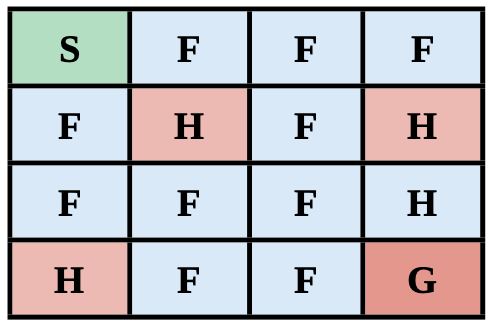
\includegraphics[width=0.35\linewidth]{frozenlake-table.png}
\caption{Frozen Lake Environment Grid}
\label{tab:frozen_lake}
\end{figure}


% \begin{table}[ht]
%     \centering
%     \setlength{\arrayrulewidth}{0.5mm}
%     \setlength{\tabcolsep}{12pt}
%     \renewcommand{\arraystretch}{1.5}
%     \begin{tabular}{|c|c|c|c|}
%         \hline
%         \cellcolor[HTML]{A9DFBF}\textbf{S} & \cellcolor[HTML]{D6EAF8}\textbf{F} & \cellcolor[HTML]{D6EAF8}\textbf{F} & \cellcolor[HTML]{D6EAF8}\textbf{F} \\ \hline
%         \cellcolor[HTML]{D6EAF8}\textbf{F} & \cellcolor[HTML]{F5B7B1}\textbf{H} & \cellcolor[HTML]{D6EAF8}\textbf{F} & \cellcolor[HTML]{F5B7B1}\textbf{H} \\ \hline
%         \cellcolor[HTML]{D6EAF8}\textbf{F} & \cellcolor[HTML]{D6EAF8}\textbf{F} & \cellcolor[HTML]{D6EAF8}\textbf{F} & \cellcolor[HTML]{D6EAF8}\textbf{H} \\ \hline
%         \cellcolor[HTML]{F5B7B1}\textbf{H} & \cellcolor[HTML]{D6EAF8}\textbf{F} & \cellcolor[HTML]{D6EAF8}\textbf{F} & \cellcolor[HTML]{F1948A}\textbf{G} \\ \hline
%     \end{tabular}
%     \caption{Frozen Lake Environment Grid}
%     \label{tab:frozen_lake} % This label is used to reference the table
% \end{table}


\begin{table*}[ht]
    \centering
    \small
    \begin{tabular}{|>{\centering\arraybackslash}p{3cm}|p{3.5cm}|p{9cm}|}
        \hline
        \textbf{Component of Markov Decision Process Formulation} & \textbf{Frozen Lake Example} & \textbf{Large Scale Recommendation Systems for Ad Policy Optimization} \\ 
        \hline
        \textbf{Environment} & The frozen lake. & The users. \\ 
        \hline
        \textbf{Goal} & Reach the goal (G) from the start position (S) while avoiding holes (H). The agent must avoid falling into a hole, and reaching the goal faster is rewarded. & Maximize revenue without compromising user experience. \\ 
         \hline
          \textbf{Episode} & A game. & A time period (T), typically 2 weeks, corresponding to an A/B experiment where enough data is collected to evaluate policy performance across users. \\ 
        \hline
        \textbf{Rewards} & Rewarded for reaching the goal (i.e., +100), but penalized for delays (i.e., -1 per step). & 
        The reward is typically represented by a utility function, which could be a weighted sum of metrics like user engagement (clicks, time spent) and revenue generated (ad clicks, conversions). The challenge lies in balancing short-term revenue with long-term user retention. \\ 
        \hline
        \textbf{Agent} & The learner. & The Recommendation System. \\ 
        \hline
        \textbf{Actions} & Up, down, left and right. & 
        Basically infinite. But when it comes to ad recommendations specifically, some typical actions are the following: 
        \begin{itemize}
            \item Reserve Price Floor: The minimum price at which an ad impression is sold.
            \item Displacement Cost Threshold: A measure of the opportunity cost for showing an ad.
            \item Max Ad Load: The maximum number of ads that can be shown without reducing user satisfaction.
            \item Ad Quality Thresholds: Standards used to ensure ads meet a quality bar before being shown.
            \item Ad Placement: The specific position of ads within the user feed (e.g., first, third, or fifth position).
        \end{itemize} \\
        \hline
        \textbf{States} & All possible grid positions the agent can occupy, representing the state space of the environment. & 
        \textbf{Signals}:
        \begin{itemize}
            \item User Context: Demographics, user profile
            \item Interaction Data: Previous interactions with ads, organic content
            \item Contextual Features: Time of day, browsing context
            \item Embeddings: Latent feature representations of user interests or ad features
        \end{itemize} \\
        \hline
        \textbf{Policy} & A mapping of grid positions to optimal action to take for a maximum reward. & 
        A mapping of user segments to ad treatments to maximize both revenue and user experience. This policy can be dynamically adjusted based on real-time feedback or offline simulations. \\ 
        \hline
    \end{tabular}
    \caption{Comparison of Frozen Lake Example and Large-Scale Recommendation Systems for Ad Policy Optimization}
    \label{tab:comparison}
\end{table*}

\subsection{The Agent and its Objective}
While toy examples like GridWorld \cite{Sutton1998}  and Frozen Lake \cite{frozenlake} provide well-defined, relatively simple environments where RL algorithms can be easily tested, transitioning these insights to real-world recommendation systems is far more complex due to factors like vast state–action spaces and delayed rewards, and environment observability \cite{dulac2019challenges, kaelbling1996reinforcement}. \textbf{Observability refers to the degree to which an agent can directly perceive the complete state of the environment} \cite{kaelbling1998planning}. In fully observable settings (such as the FrozenLake), the agent sees the true state at every step, enabling straightforward decision-making \cite{kaelbling1998planning}. However, real-world environments, including \textbf{recommendation systems, are often partially observable \cite{lu2016partially}}; the agent must infer the underlying state from incomplete or noisy signals, increasing both the computational complexity of learning and the uncertainty of policy outcomes \cite{wu2021partially}. In the FrozenLake environment, the \textbf{agent is a decision-maker that observes its surroundings and chooses actions}. It learns to navigate the grid to reach the goal (\textcolor[HTML]{FF4500}{G}) from the start position (\textcolor[HTML]{228B22}{S}) while avoiding holes (\textcolor[HTML]{FF0000}{H}) and navigating slippery surfaces (\textcolor[HTML]{1E90FF}{F}). By analogy, in ad policy optimization, \textbf{the agent is the algorithm responsible for serving ads}, which must balance two primary \textbf{objectives}: maximizing revenue while maintaining (or ideally enhancing) user engagement \cite{Theocharous-2015, zou2019reinforcement}. Ultimately, both the FrozenLake agent and the ad-serving algorithm share the same high-level goal: to maximize long-term rewards through strategic actions grounded in observed states.

The use of a \textbf{reward signal} to formalize the idea of a goal is a distinctive feature of RL \cite{Sutton1998}. In an MDP, the reward is a scalar value the agent receives after taking an action in a given state and transitioning to a new state, serving as immediate feedback on the benefit or cost of the action \cite{kaelbling1996reinforcement}. This feedback allows the agent to learn a policy that maximizes the cumulative reward over time \cite{kaelbling1996reinforcement}. In simple RL scenarios, rewards are typically straightforward. For instance, the agent might receive -1 per move (to encourage shorter paths), +100 for reaching the goal (G), and -100 if it falls into a hole (H), ending the episode. \textbf{However, in real-world recommendation systems, reward structures can be far more nuanced.  It is often unclear which user behaviors warrant the highest reward or how to weigh different signals} \cite{mcdonald2023spotify}. In online advertising, for example, low-intent actions such as clicks may be valued less than high-intent actions like saves or purchases. Moreover, deciding how to balance these varied signals in a single reward function can be both subjective and complex, especially when multiple objectives (e.g., revenue, user satisfaction, and content diversity) must be optimized \cite{mcdonald2023spotify}.\\

Ad recommendation engines often need to \textbf{balance multiple objectives}, such as maximizing user engagement while also ensuring ad revenue \cite{zhang2018whole, yan2020ads, sagtani2024ad}. Long-term engagement and revenue are metrics that are particularly difficult to measure directly, especially in randomized controlled experiments that typically span only a couple of weeks \cite{mcdonald2023spotify}. The delay in outcomes (e.g., retention signals may take months to manifest) and the often subtle impact of a single intervention can make it nearly impossible to detect meaningful changes within such short time frames \cite{mcdonald2023spotify}.  As a result, proxy metrics are commonly used. For instance, click-through rate (CTR) and ad impressions serve as approximate measures of revenue, while session duration, saves, and shares act as proxies for longer-term engagement \cite{wang2022surrogate}. However, these simpler proxies can fail to capture the system’s true long-term objectives, occasionally leading to suboptimal policies \cite{mazoure2021improving}. A high CTR may reflect short-term engagement, yet it can ultimately induce ad fatigue or frustrate users if the ads are misaligned with their actual interests \cite{hohnhold2015focusing, sagtani2024ad}. Table \ref{fig:proxy-metrics} summarizes some of the most commonly used proxies in the industry across dimensions of revenue, engagement, and ad fatigue. 


% \begin{figure}[H]
% \centering
% 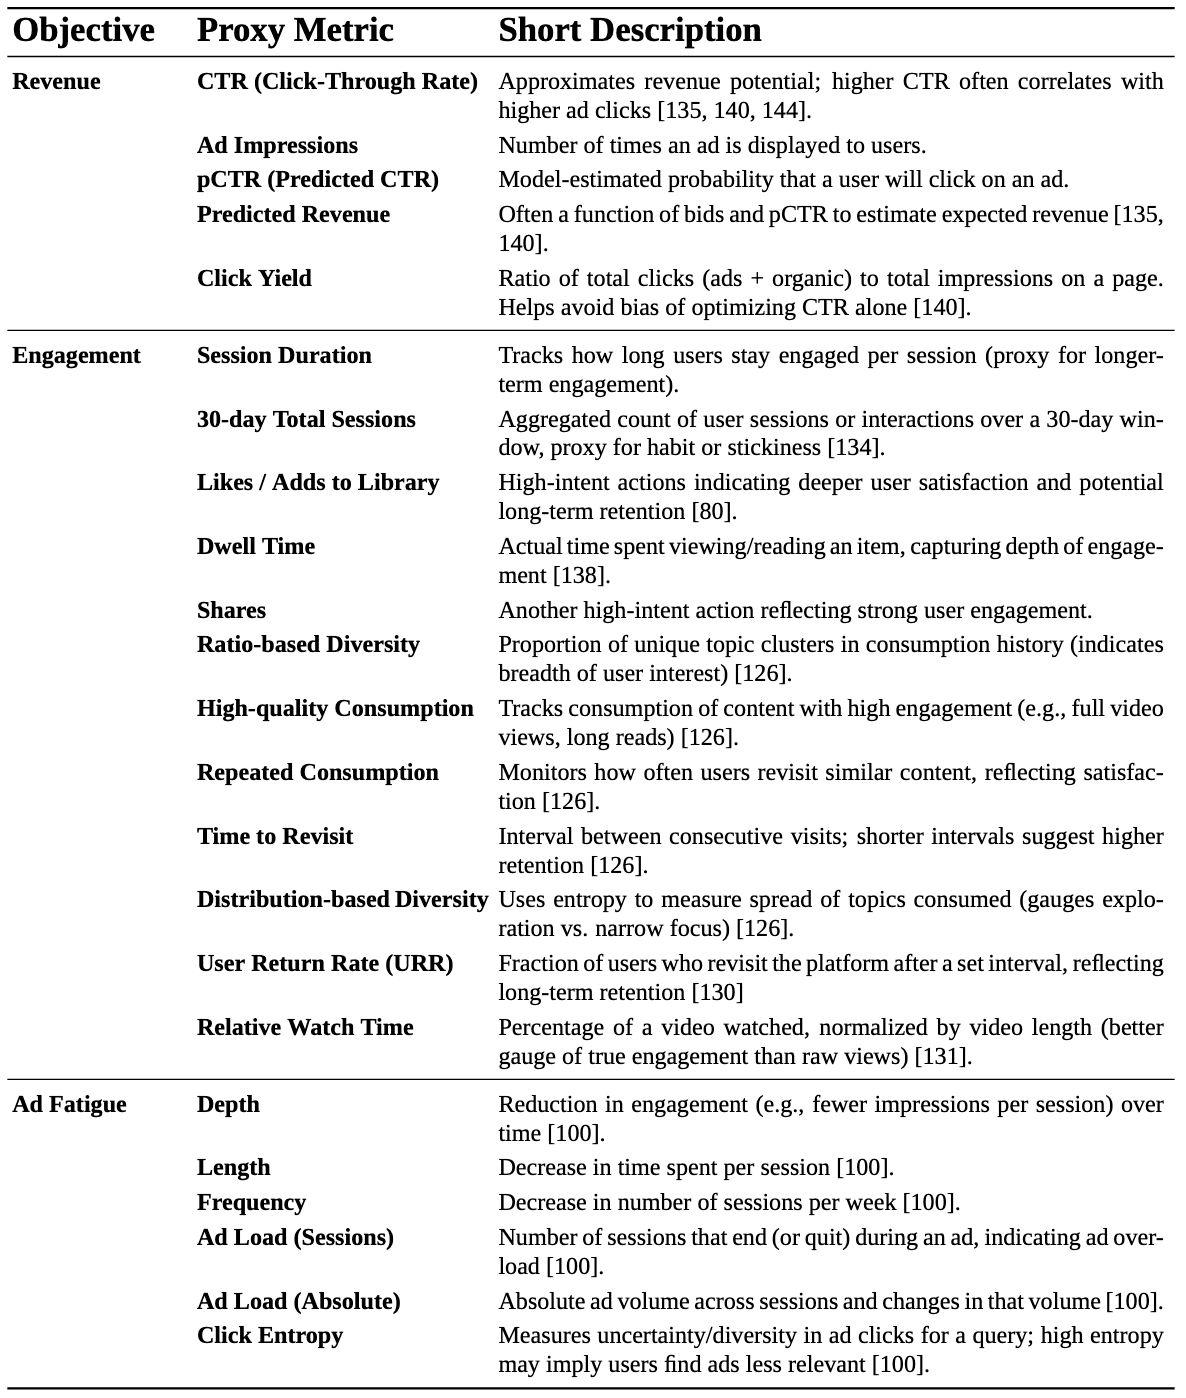
\includegraphics[width=\linewidth]{proxy-metrics-table.png}
% \caption{Proxy metrics for Revenue, Engagement, and Ad Fatigue.}
% \label{fig:proxy-metrics}
% \end{figure}

\begin{figure}[ht]
  \centering
  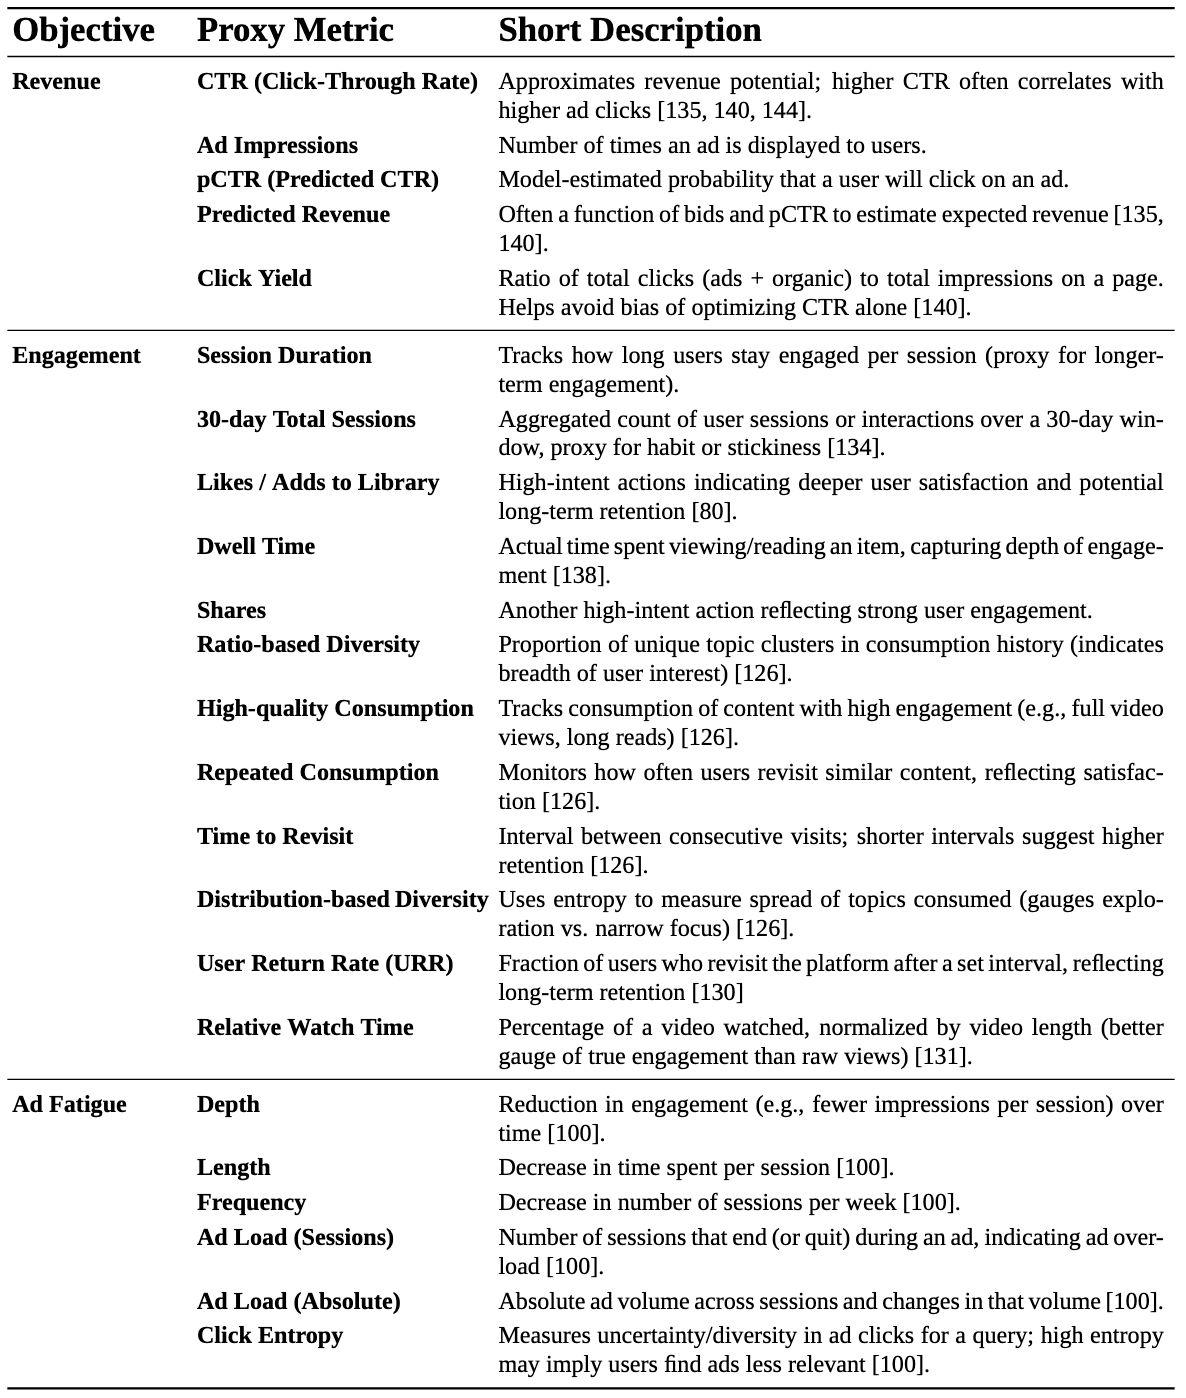
\includegraphics[width=\textwidth, height=0.85\textheight, keepaspectratio]{proxy-metrics-table.png}
  \caption{Proxy metrics for Revenue, Engagement, and Ad Fatigue.}
  \label{fig:proxy-metrics}
\end{figure}


% \begin{table}[H]
% \setstretch{1} % Ensure normal spacing within table. Separation between lines of the same cell. 
% \centering
% \small
% \renewcommand{\arraystretch}{1.2}  % Tweak if needed
% \setlength{\tabcolsep}{2pt} % separation between columns 
% \begin{tabularx}{\linewidth}{p{0.15\linewidth} p{0.25\linewidth} p{0.57\linewidth}}
% % the decimal points allow to control the size of the table, not of the text.
% \toprule
% {\bfseries \Large Objective} & {\bfseries \Large Proxy Metric} & {\bfseries \Large Short Description} \\
%   % \textbf{Objective} & \textbf{Proxy Metric} & \textbf{Short Description} \\
% \midrule
%     \multirow{\textbf{Revenue}} 
%        & \textbf{CTR (Click-Through Rate)} 
%            &  Approximates revenue potential; higher CTR often correlates with higher ad clicks \cite{zhang2018whole, yan2020ads, zhao2020jointly}. \\
%        & \textbf{Ad Impressions} 
%            & Number of times an ad is displayed to users. \\
%        & \textbf{pCTR (Predicted CTR)} 
%            & Model-estimated probability that a user will click on an ad. \\
%        & \textbf{Predicted Revenue} 
%            & Often a function of bids and pCTR to estimate expected revenue  \cite{yan2020ads, zhang2018whole}. \\
%        & \textbf{Click Yield} 
%            & Ratio of total clicks (ads + organic) to total impressions on a page. Helps avoid bias of optimizing CTR alone \cite{zhang2018whole}. \\
%     \midrule
%     \multirow{\textbf{Engagement}} 
%        & \textbf{Session Duration} 
%            & Tracks how long users stay engaged per session (proxy for longer-term engagement). \\
%         & \textbf{30-day Total Sessions} 
%        & Aggregated count of user sessions or interactions over a 30-day window, proxy for habit or stickiness 
%        \cite{xu2023optimizing}. \\
%        & \textbf{Likes / Adds to Library} 
%        & High-intent actions indicating deeper user satisfaction and potential long-term retention \cite{mcdonald2023spotify}. \\
%           & \textbf{Dwell Time} 
%        & Actual time spent viewing/reading an item, capturing depth of engagement  \cite{yi2014beyond}. \\
%        & \textbf{Shares} 
%            & Another high-intent action reflecting strong user engagement. \\
%     & \textbf{Ratio-based Diversity}  
%            & Proportion of unique topic clusters in consumption history (indicates breadth of user interest) \cite{wang2022surrogate}. \\
%        & \textbf{High-quality Consumption} 
%            & Tracks consumption of content with high engagement (e.g., full video views, long reads) \cite{wang2022surrogate}. \\
%      & \textbf{Repeated Consumption}  
%            & Monitors how often users revisit similar content, reflecting satisfaction \cite{wang2022surrogate}. \\
%               & \textbf{Time to Revisit} 
%            & Interval between consecutive visits; shorter intervals suggest higher retention \cite{wang2022surrogate}. \\
%      & \textbf{Distribution-based Diversity}  
%            & Uses entropy to measure spread of topics consumed (gauges exploration vs. narrow focus) \cite{wang2022surrogate}. \\
%     & \textbf{User Return Rate (URR)} 
%        & Fraction of users who revisit the platform after a set interval, reflecting long-term retention  \cite{wu2017returning} \\
%      & \textbf{Relative Watch Time} 
%        & Percentage of a video watched, normalized by video length (better gauge of true engagement than raw views) 
%       \cite{wu2018beyond}. \\
%     \midrule
%     \multirow{\textbf{Ad Fatigue}} 
%        & \textbf{Depth} 
%            & Reduction in engagement (e.g., fewer impressions per session) over time \cite{sagtani2023quantifying}. \\
%        & \textbf{Length} 
%            & Decrease in time spent per session \cite{sagtani2023quantifying}. \\
%        & \textbf{Frequency} 
%            & Decrease in number of sessions per week \cite{sagtani2023quantifying}. \\
%        & \textbf{Ad Load (Sessions)} 
%            & Number of sessions that end (or quit) during an ad, indicating ad overload \cite{sagtani2023quantifying}. \\
%        & \textbf{Ad Load (Absolute)} 
%            & Absolute ad volume across sessions and changes in that volume \cite{sagtani2023quantifying}. \\
%        & \textbf{Click Entropy} 
%            & Measures uncertainty/diversity in ad clicks for a query; high entropy may imply users find ads less relevant \cite{sagtani2023quantifying}. \\
% \bottomrule
% \end{tabularx}
% \caption{Proxy metrics for Revenue, Engagement, and Ad Fatigue.}
% \label{tab:proxy-metrics}
% \end{table}




\textbf{Utility functions are mathematical constructs used to estimate the net value of conflicting objectives \cite{Stigler1950}.} A utility function is a \textbf{composite reward function} that allows the agent to integrate various rewards or metrics from multiple objectives using a unified currency, facilitating more nuanced decision-making across competing priorities \cite{Stigler1950}. The ability to compare two utilities, like those of revenue and engagement normalized to a common scale, is critical for any principled blending of organic items and ads \cite{yan2020ads}.  Most utility functions are linear though this linearity is not a requirement for how the individual utility of each component is calculated \cite{wen2019learning, zhao2020jointly}. 

A \textbf{canonical utility function} at the policy layer to \textit{blend} ads and organic content can be represented as follows \cite{sagtani2024ad, yan2020ads, carrion2021blending}:
    \begin{equation}
        U(x) = \alpha \times \text{Revenue} + \beta \times \text{Engagement} - \gamma \times \text{Ad Fatigue}
    \end{equation}
    where $\alpha$, $\beta$, and $\gamma$ are weights that determine the relative importance of each factor. To compute the utilities of "Revenue", "Engagement", and "Ad Fatigue", typically many signals feed into each component. These signals include, but are not limited to, the ones shown in Table \ref{fig:proxy-metrics}. In a bandit or RL context, $U(x)$ serves as the reward signal guiding policy updates. The process of tuning the weights of $\alpha$, $\beta$, and $\gamma$ is often done through experimentation, as the right balance between engagement and revenue can shift depending on the context. For instance, ByteDance uses a multi-objective reward framework in their recommendation systems, where different reward functions are designed for organic content and ads, combining them to guide the overall recommendation strategy \cite{zhao2020jointly}.
    
In some cases, a very simple unified function can suffice over a complex utility function. Researchers at Alibaba introduced the concept of Click Yield, which is defined as the ratio of the total number of clicks on all items (ads + organic results) to the total number of impressions on a page \cite{zhang2018whole}. Click Yield provides a holistic evaluation of page performance, accounting for the interactive effects between ads and organic content, and helping to mitigate the bias that arises from examining CTR in isolation. Their optimization task maximizes total revenue while ensuring that the Click Yield does not fall below a certain threshold (T)  \cite{zhang2018whole}. A comparison of utility function formulations is shown in Table \ref{fig:utility-comparison}.

\begin{figure}[ht]
\centering
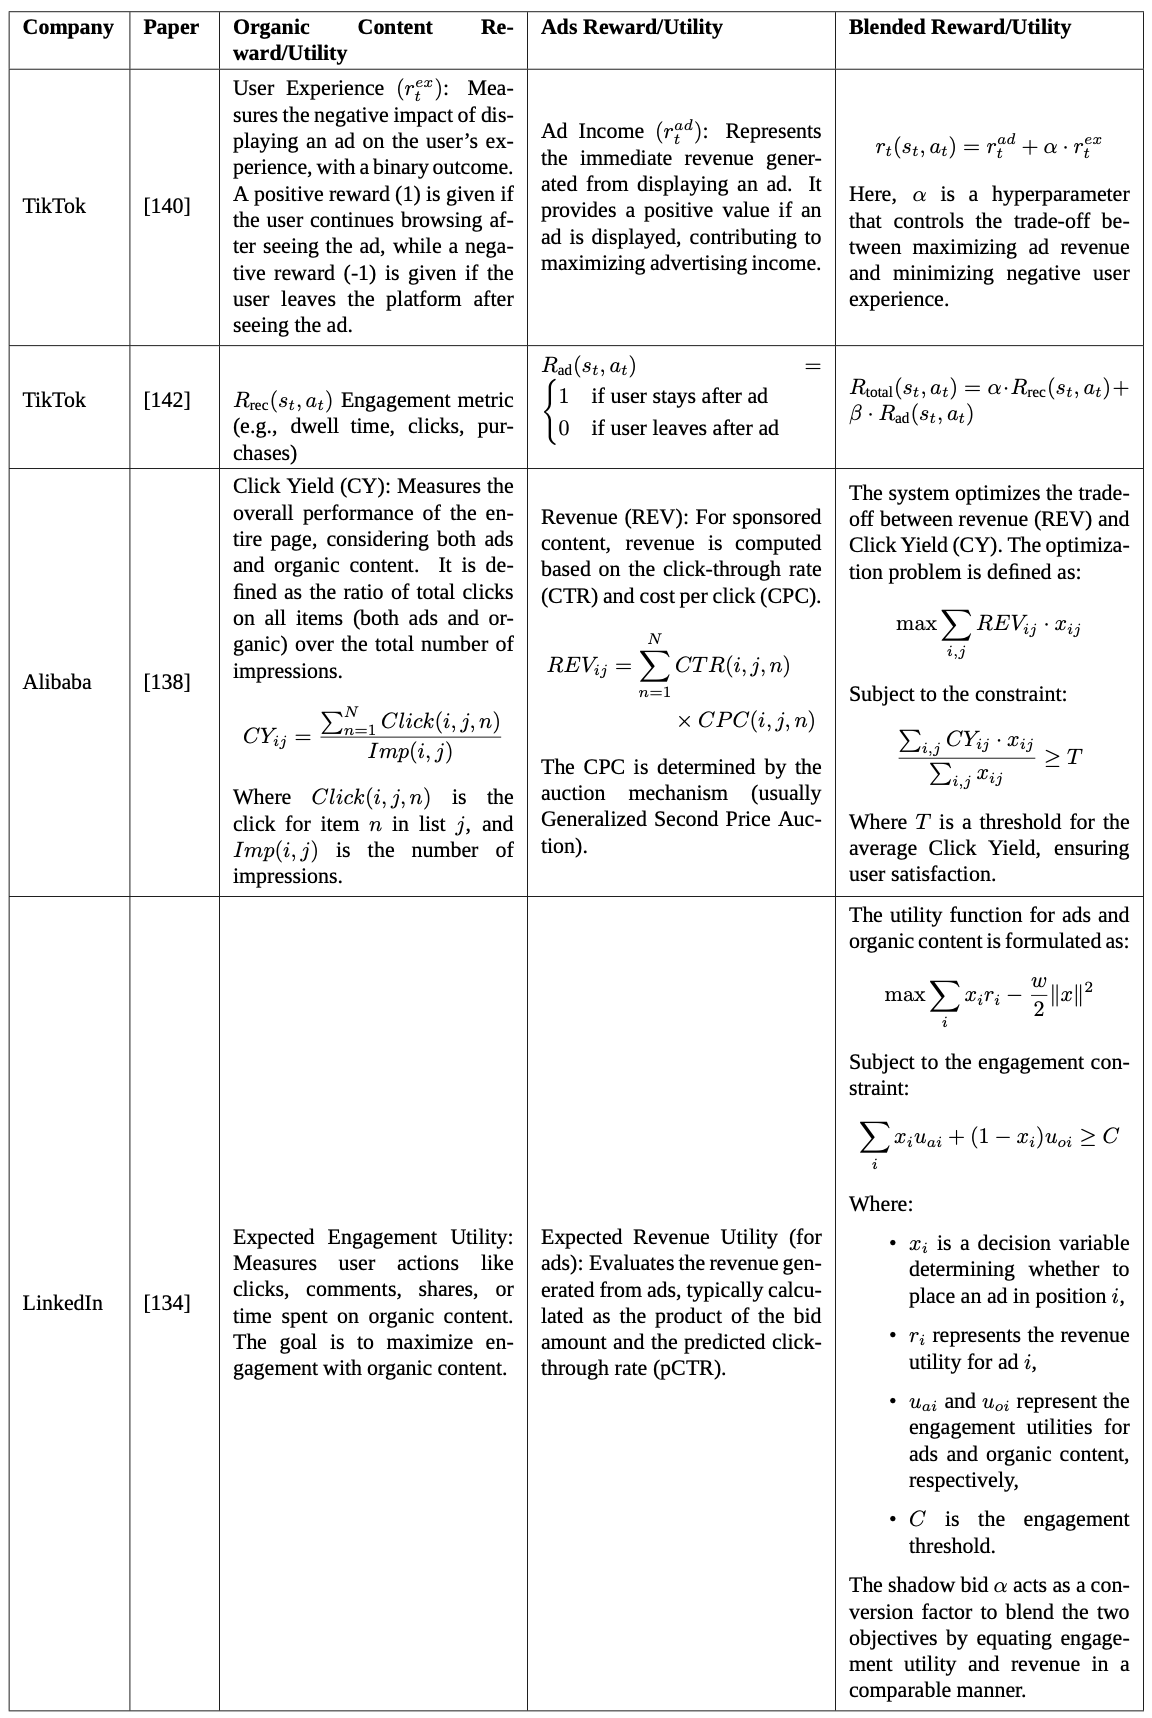
\includegraphics[width=\textwidth, height=0.85\textheight, keepaspectratio]{utility-comparison-table.png}
\caption{Comparison of Utility/Reward Formulation Approaches across Different Companies}
\label{fig:utility-comparison}
\end{figure}



% Adjusted table with better column width control and proper spacing
% \begin{table}[ht]
%     \centering
%     % \renewcommand{\arraystretch}{1.3}  % Adjust row height spacing
%     \begin{adjustbox}{max width=\textwidth}
%     \small % Decrease font size for the table
%     % \setlength{\tabcolsep}{6t} % Increase spacing between text and vertical lines
%     \renewcommand{\arraystretch}{1.15}
% \begin{tabular}{|p{1.5 cm}|p{1 cm}|p{4.5 cm}|p{4.5 cm}|p{4.5 cm}|}
%     \hline
%     \textbf{Company} & \textbf{Paper} & \textbf{Organic Content Reward/Utility} & \textbf{Ads Reward/Utility} & \textbf{Blended Reward/Utility} \\ 
%     \hline
%     TikTok & \cite{zhao2021dear} & 
%     \begin{minipage}{4.5cm}
%     \vspace{4pt}
%         User Experience \((r_t^{ex})\): Measures the negative impact of displaying an ad on the user's experience, with a binary outcome. A positive reward (1) is given if the user continues browsing after seeing the ad, while a negative reward (-1) is given if the user leaves the platform after seeing the ad.
%         \vspace{4pt}
%     \end{minipage}
%     & 
%     \begin{minipage}{4.5cm}
%     \vspace{4pt}
%         Ad Income \((r_t^{ad})\): Represents the immediate revenue generated from displaying an ad. It provides a positive value if an ad is displayed, contributing to maximizing advertising income.
%         \vspace{4pt}
%     \end{minipage}
%     & 
%     \begin{minipage}{4.5cm}
%     \vspace{4pt}
%         \[
%         r_t(s_t, a_t) = r_t^{ad} + \alpha \cdot r_t^{ex}
%         \]
%         Here, \(\alpha\) is a hyperparameter that controls the trade-off between maximizing ad revenue and minimizing negative user experience.
%         \vspace{4pt}
%     \end{minipage} \\
%     \hline
%     TikTok & \cite{zhao2020jointly} & 
%     $R_{\text{rec}}(s_t, a_t)$ Engagement metric (e.g., dwell time, clicks, purchases)  
%     & 
%     \begin{minipage}{4.5cm}
%     \vspace{4pt} 
%     \( R_{\text{ad}}(s_t, a_t) = 
%     \begin{cases} 
%         1 & \text{if user stays after ad} \\
%         0 & \text{if user leaves after ad} 
%     \end{cases} \) 
%         \vspace{4pt}
%     \end{minipage}
%     & 
%     \begin{minipage}{4.5cm}
%     \vspace{4pt}
%     \( R_{\text{total}}(s_t, a_t) = \alpha \cdot R_{\text{rec}}(s_t, a_t) + \beta \cdot R_{\text{ad}}(s_t, a_t) \)
%         \vspace{4pt}
%     \end{minipage} \\
%     \hline
%     Alibaba & \cite{zhang2018whole} & 
%     \begin{minipage}{4.5cm}
%     \vspace{4pt}
%         Click Yield (CY): Measures the overall performance of the entire page, considering both ads and organic content. It is defined as the ratio of total clicks on all items (both ads and organic) over the total number of impressions.
%         \[
%         CY_{ij} = \frac{\sum_{n=1}^{N} Click(i, j, n)}{Imp(i, j)}
%         \]
%         Where \(Click(i, j, n)\) is the click for item \(n\) in list \(j\), and \(Imp(i, j)\) is the number of impressions.
%         \vspace{4pt}
%     \end{minipage}
%     & 
%     \begin{minipage}{4.5cm}
%     \vspace{4pt}
%         Revenue (REV): For sponsored content, revenue is computed based on the click-through rate (CTR) and cost per click (CPC).
%         \[
% \begin{aligned}
% REV_{ij} = \sum_{n=1}^{N} & \, CTR(i, j, n) \\
% & \times CPC(i, j, n)
% \end{aligned}
% \]
%         The CPC is determined by the auction mechanism (usually Generalized Second Price Auction).
%         \vspace{4pt}
%     \end{minipage}
%     & 
%     \begin{minipage}{4.5cm}
%     \vspace{4pt}
%         The system optimizes the trade-off between revenue (REV) and Click Yield (CY). The optimization problem is defined as:
%         \[
%         \max \sum_{i,j} REV_{ij} \cdot x_{ij}
%         \]
%         Subject to the constraint:
%         \[
%         \frac{\sum_{i,j} CY_{ij} \cdot x_{ij}}{\sum_{i,j} x_{ij}} \geq T
%         \]
%         Where \(T\) is a threshold for the average Click Yield, ensuring user satisfaction.
%         \vspace{4pt}
%     \end{minipage} \\
%     \hline
%     LinkedIn & \cite{yan2020ads} & 
%     \begin{minipage}{4.5cm}
%     \vspace{4pt}
%         Expected Engagement Utility: Measures user actions like clicks, comments, shares, or time spent on organic content. The goal is to maximize engagement with organic content.
%         \vspace{4pt}
%     \end{minipage}
%     & 
%     \begin{minipage}{4.5cm}
%     \vspace{4pt}
%         Expected Revenue Utility (for ads): Evaluates the revenue generated from ads, typically calculated as the product of the bid amount and the predicted click-through rate (pCTR).
%         \vspace{4pt}
%     \end{minipage}
%     & 
%     \begin{minipage}{4.5cm}
%     \vspace{4pt}
%         The utility function for ads and organic content is formulated as:
%         \[
%         \max \sum_i x_i r_i - \frac{w}{2} \| x \|^2
%         \]
%         Subject to the engagement constraint:
%         \[
%         \sum_i x_i u_{ai} + (1 - x_i) u_{oi} \geq C
%         \]
%         Where:
%         \begin{itemize}
%             \item \(x_i\) is a decision variable determining whether to place an ad in position \(i\),
%             \item \(r_i\) represents the revenue utility for ad \(i\),
%             \item \(u_{ai}\) and \(u_{oi}\) represent the engagement utilities for ads and organic content, respectively,
%             \item \(C\) is the engagement threshold.
%         \end{itemize}
%         The shadow bid \(\alpha\) acts as a conversion factor to blend the two objectives by equating engagement utility and revenue in a comparable manner.
%         \vspace{4pt}
%     \end{minipage} \\
%     \hline
% \end{tabular}
% \end{adjustbox}
% \caption{Comparison of Utility/Reward Formulation Approaches across Different Companies}
% \label{tab:utility-comparison}
% \end{table}


\subsection{Action Space Representation}
\label{action_space_representation}

In RL, environments are modeled as a Markov Decision Process (MDP). An MDP is defined by $(\mathcal{S}, \mathcal{A}, P, R)$, where $\mathcal{S}$ is the state space, $\mathcal{A}$ is the action space, $P(\cdot\mid s,a)$ is the transition probability distribution, and $R(s,a)$ is the reward function. At each timestep $t$, the agent observes a state $s_t \in \mathcal{S}$ and selects an action $a_t \in \mathcal{A}$. Both action and state sets may be finite, infinite, discrete, or continuous.

% What is an action 
In RL, an \textbf{action} $a \in \mathcal{A}$ refers to \textbf{a decision or intervention taken by the agent based on its current state to influence the environment} \cite{Sutton1998}. The action space $\mathcal{A}$  represents the complete set of all possible actions that the agent can choose from at any given decision point \cite{Sutton1998}. For example, in the  FrozenLake environment,\textbf{ the possible actions for the agent are \textit{up, down, left} and \textit{right}} \cite{frozenlake}. \textbf{Because this set of possible actions is countable, the action space for the FrozenLake is said to be \textit{discrete} \cite{frozenlake}.} By contrast, in an \emph{advertisement recommendation} setting, the action space $\mathcal{A}$ might consist of all possible combinations of ads, their rankings, placements, and formats \cite{ie2019slateq}. The objective of this set of actions in ad recommendation is to deliver the right set of ads at the right time in order to maximize platform revenue, while maintaining or improving user engagement and satisfaction \cite{zhao2020jointly}. Although this action space is discrete and countable, the number of possible combinations grows exponentially with the number of candidate ads and available slots. As a result, it becomes computationally infeasible to enumerate or evaluate each action individually, and must instead be treated using methods designed for high-dimensional discrete spaces \cite{ie2019recsim}.

\textbf{An ideal action space should be \textit{expressive} enough to capture all relevant degrees of freedom the agent needs to optimize its behavior, but it should avoid unnecessary complexity \cite{zhu2024discretizing, liu2025reducing}.} The action space described above in the FrozenLake example satisfies these criteria, as the four cardinal movements (\textit{up, down, left,} and \textit{right}) are enough to navigate to any state in the grid while remaining \textbf{orthogonal}, thus providing both sufficient \textbf{coverage and simplicity} \cite{frozenlake}.  In contrast, the ad recommendation action space is inherently high-dimensional and entangled \cite{ie2019recsim}. The agent must decide \emph{what} to show (a discrete choice over candidate ads), \emph{where} to place it  (which may be modeled as a discrete slot or a continuous position), and in \emph{what order} (often determined by continuous relevance scores), often under tight latency constraints and user personalization requirements \cite{zhao2020jointly}. The action space in ad recommendation systems must be expressive enough to encompass all relevant choices for optimal ad delivery while ensuring no combinatorial explosion in complexity \cite{ie2019slateq}. Moreover, ensuring that each dimension remains sufficiently \emph{orthogonal} can be nontrivial, given potential interactions between ad content, positioning, and user context \cite{ie2019reinforcement}. If the action space is too coarse, the system risks underfitting, serving generic policies that fail to personalize effectively or miss monetization opportunities \cite{ie2019slateq}. On the other hand, if it is too fine, the system may overfit to noise, struggle to generalize, or incur prohibitive computational costs \cite{ie2019slateq}. Practical systems often resort to action abstraction or parameterization (e.g., slate-based policies, ad load knobs, or policy buckets) to reduce complexity at the cost of optimality \cite{ie2019reinforcement, hohnhold2015focusing, sagtani2024ad}.

\textbf{The independence of these action dimensions facilitates more modular policy learning \cite{tavakoli2018action, sharma2017learning}}. By allowing a degree of independence for each action dimension, the agent achieves modular policy learning that scales linearly (instead of exponentially) with the number of action degrees-of-freedom \cite{tavakoli2018action}. In addition, actions should ideally correspond to \textbf{semantically meaningful choices} to facilitate policy interpretability and validation \cite{glanois2024survey, puiutta2020explainable}. In the case of the FrozenLake problem, the action space is intuitive and human-interpretable, making it straightforward to validate learned policies \cite{brockman2016openai, Sutton1998}. For instance, an RL practitioner can manually inspect and reason about the learned policy (e.g. "the agent plans to move \textit{down} then \textit{right} to reach the goal") to verify that each action choice aligns with domain logic \cite{brockman2016openai}. While the action space in ad recommendation systems is far more complex, structuring it around semantically meaningful levers (e.g., “increase ad load for high-intent users” or “downrank low-quality creatives”) enables engineers and product teams to reason about the system’s behavior \cite{glanois2024survey, dulac2021challenges}. If a learned policy increases ad load for a particular user segment, analysts can trace this decision back to upstream signals, such as historical engagement patterns or commercial intent scores \cite{gauci2018horizon, dulac2021challenges}. Policies composed of interpretable levers enable more transparent debugging, offline validation, and policy review, which is crucial for ensuring that the deployed strategy aligns with business intuition, avoids learning spurious correlations, and mitigates the risk of unintended outcomes \cite{dulac2021challenges, verma2018programmatically, puiutta2020explainable, glanois2024survey}.

\textbf{Moreover, an action space should be consistent across episodes \cite{puterman2014markov}.} That is, taking the same action in the same state should yield statistically predictable outcomes \cite{puterman2014markov}. \textbf{The state space in the FrozenLake is stochastic \cite{frozenlake}}, meaning that taking the same action does not always result in the same next state. For example, selecting the action "move right" might result in the agent moving right, up, or down, as governed by the transition probabilities defined by $P(s' \mid s, a)$ \cite{frozenlake}. Despite the stochasticity in the environment,\textbf{ the outcomes observed should converge to the expected values described by the transition probability distribution over a sufficiently large number of episodes \cite{puterman2014markov}}. A similar principle applies in ad recommendation. Although user behavior and auction dynamics introduce stochasticity, \textbf{taking the same ad-serving action, such as presenting a specific slate of ads to a user with a given context, should yield statistically predictable engagement or monetization outcomes}. That is, over many episodes, \textbf{the distribution of observed rewards (e.g., clicks, conversions, revenue) should converge to the expected value associated with the given state-action pair \cite{mcmahan2013ad, zhao2018deep}}. This consistency is foundational for policy learning, as it ensures that repeated exposure to similar decision contexts enables accurate estimation of long-term value, despite noisy observations \cite{Sutton1998}. 

The action space can be thought of as levers that can be used to tune ad policy. Typical \textbf{levers in treatments in ad policies} include the following elements \cite{koutsopoulos2016native}: 

\begin{itemize}
    \item \textbf{Ad Load.} Also referred to as the spacing ads or frequency of ads is also a key component in inducing ad load fatigue. Placing ads too closely together may lead to user fatigue and reduced click probabilities \cite{abrams2007personalized, zhao2020jointly}. 
    \item \textbf{Ad Quality.} This refers to intrinsic features of the ad, such as the design format, product type, accompanying text, and the quality of the landing page, all of which directly influence user engagement. \cite{yan2009much, nielsen2017advertising}.
    \item \textbf{Ad Placement.}
Ads placed earlier in the feed are more likely to be clicked, though their relevance to preceding content also plays a significant role \cite{zhao2020jointly, saha2021advertiming, yuan2020unbiased}. 
    \item \textbf{Ad Relevance.} Ads that align more closely with user preferences and user intent are more likely to drive engagement. For example, an ad on a hotel might have a higher probability if shown adjacent to results of search queries related to vacations \cite{chakrabarti2008contextual, Zhou2018}. \\
\end{itemize}

\subsection{State Space Representation} \label{state_space_representation}
% Definition and Desirable Properties
% 1.1 What is a state space in RL?
% 1.2 Desirable properties of a state space
% Markovianity
% Expressiveness vs. generalization
% Stability under distribution shift
% Sample efficiency and learnability
% Interpretability and support for counterfactual reasoning

In RL, a \textit{state} $s \in \mathcal{S}$  represents all the relevant information from past agent-environment interactions necessary for the agent to make optimal decisions to maximize the expected cumulative reward \cite{Sutton1998}. Ideally, the state space is Markovian, meaning the future is conditionally independent of the past given the current state \cite{russell2016artificial, Sutton1998}. If the agent’s policy or value estimates rely on omitted or unobserved information from the past, the state representation violates the Markov property and the performance of the learned policy may degrade as a result \cite{russell2016artificial, Sutton1998}. In the FrozenLake example, the state space consists of the agent’s current grid position as the future outcomes of any action depend only on this position, and not on how the agent arrived there \cite{frozenlake}. In this example, because future transitions depend only on the current state and action, and not on prior history, the FrozenLake Environment satisfies the \textit{Markov Property} \cite{Sutton1998, frozenlake}.  


In contrast, the environments where \textbf{ad recommendation systems} operate are often \textbf{partially observable, high-dimensional, and non-stationary} \cite{dulac2021challenges, russell2016artificial}. To construct a state representation that reasonably approximates the Markov property in the face of partial observability and complex user dynamics, ad recommendation systems often combine tabular features with learned embeddings \cite{afsar2022reinforcement, kaelbling1998planning}. The tabular signals tend to include static attributes (e.g. demographics), contextual metadata (e.g. device type, time of the day), and behavioral history (e.g. recent clicks, impressions, or dwell time) \cite{cheng2016wide, covington2016deep}. An embedding is a learned, dense vector that encodes complex or high-cardinality inputs, such as user profiles, ads, or behavioral sequences, into a lower-dimensional space \cite{cheng2016wide}. Compared to static tabular features like frequency counts or recency buckets, embeddings capture richer structure, including sequence effects and latent similarity. This makes them more expressive and task-relevant, enabling ad recommendation systems to personalize content and ads more effectively \cite{covington2016deep, cheng2016wide}.

% User embeddings, item embeddings, user-item interaction embeddings, and sequence embeddings are among the most common embedding types used in recommendation systems. Each embedding type captures distinct aspects of information to guide the agent’s decisions. 

% Contextual features, including a user's location or device type, often serve as informative priors, particularly helpful in addressing the cold-start problem, i.e., when new users enter an ecosystem with limited historical data \cite{covington2016deep}. Additionally, some platforms prompt new users to select interests or topics during onboarding, providing supplementary signals that help initialize user embeddings. When no data for users is available (incognito window, SEO-driven traffic, new device without login, etc), systems typically default to population-level trends or popular content. While user embeddings may also be static and updated on batch mode, user embeddings can also be updated dynamically, such that as users engage further, the continuous updates on the embeddings allow for more personalized policies by the agent to reflect new information in the system and evolving preferences.

Embeddings may consist of two components: an offline (stationary) component and an online (non-stationary) component \cite{zhao2023embedding}. \textbf{Offline embeddings} represent \textbf{stationary or slow-changing attributes}, such as a user's demographics (e.g., gender, country) or long-term preferences, and fixed item properties (e.g., brand or product category) \cite{koren2009matrix, quadrana2018sequence}. These embeddings are usually computed in batch mode due to their \textbf{higher computational complexity, larger size, and relatively static nature} \cite{naumov2019deep, liu2022monolith}. \textbf{Online embeddings}, conversely, address non-stationary and rapidly evolving aspects such as recent user behaviors, trending content, or immediate interests \cite{Zhou2018, zhou2019deep}. These embeddings are \textbf{generally smaller,} \textbf{computed in near-real-time to meet latency requirements} \cite{liu2022monolith}. This hybrid approach combines stable and dynamic embeddings, balancing relevance with computational efficiency \cite{cheng2016wide, covington2016deep}. Furthermore, this allows the recommendation system to remain stable under distribution shifts, which is of paramount importance, especially in environments with rapidly evolving user preferences, content inventories, and behavioral patterns \cite{gama2014survey, Sutton1998}.

To effectively integrate diverse embeddings (user, item, interaction) and their offline and online components, embeddings of varying dimensions are typically concatenated and then projected via learned linear layers into a shared dimension \cite{pancha2022pinnerformer, grbovic2018real, covington2016deep}. Generally, zero-padding or truncation is avoided, as these methods can introduce noise or cause information loss \cite{xia2023transact}.

\textbf{User embeddings} are learned vector representations designed to capture user preferences and behaviors, enabling ad recommendation systems to personalize content effectively at scale \cite{covington2016deep, he2017neural}. These embeddings compress complex, high-dimensional user data, such as past interactions and demographic information, into compact vectors utilized by recommendation models \cite{covington2016deep, koren2009matrix, naumov2019deep}. User embeddings can be learned using a combination of supervised, unsupervised, and self-supervised approaches \cite{zhao2021dear}.  In the case of supervised learning, embeddings are optimized to predict explicit labels such as clicks, conversions, or purchases \cite{covington2016deep, Zhou2018}. To exploit information in more implicit signals, self-supervised methods can be used with objectives such as next item interaction or item co-occurrence \cite{yuan2020unbiased, mikolov2013distributed}. Many practical implementations tend to combine both supervised and self-supervised methods \cite{zhao2021dear, xia2023transact}. For example, embeddings may initially be learned through self-supervised tasks (e.g., predicting next clicks) and then fine-tuned on supervised tasks (CTR, conversions). A well-documented example is that of YouTube, where despite the availability of explicit feedback mechanisms (thumbs up/down, in-product surveys, etc.), they turn to implicit signals, where a user completing a video is a positive example, given that the relative prevalence of implicit signals is much higher than explicit signals, allowing the models to learn more effectively \cite{covington2016deep}.

\textbf{Item embeddings} are designed to capture intrinsic item characteristics \cite{koren2009matrix}. These embeddings compress complex, high-dimensional item data, such as product descriptions, categories, brands, and historical interaction patterns \cite{koren2009matrix, cheng2016wide}. Similar to user embeddings, item embeddings can be learned through supervised, unsupervised, and self-supervised approaches \cite{barkan2016item2vec, zhao2023embedding}. In supervised learning scenarios, embeddings are optimized to predict explicit labels, such as clicks, conversions, or purchases associated with the items \cite{covington2016deep, naumov2019deep}. To leverage more implicit information, self-supervised methods may focus on objectives like predicting co-occurrence patterns or sequential interactions (e.g., item-to-item relationships) \cite{barkan2016item2vec, sun2019bert4rec}. 

While user and item embeddings provide essential representations of individual entities, it is through interaction embeddings, which capture the joint dynamics between users and items, that the system truly learns user preferences and can surface content that is contextually relevant and personalized \cite{koren2009matrix}. Being able to \textbf{ effectively represent user-item interactions} is at the core of personalization for recommendation systems \cite{linden2003amazon}. Collaborative Filtering (CF) was one of the earliest popular methods to represent user-item interactions \cite{linden2003amazon, Bobadilla2013}. CF predicted user preferences by analyzing explicit interactions (e.g., ratings) or implicit behavioral signals (e.g., clicks, views), using metrics like cosine similarity or Pearson correlation \cite{Bobadilla2013}. However, CF struggled with sparse datasets, as many user-item pairs lacked interactions, limiting recommendation accuracy \cite{Bobadilla2013}. Additionally, CF's direct interaction-based approach limited its ability to capture deeper latent or implicit relationships between users and items \cite{koren2008factorization}.

Matrix Factorization (MF), popularized during the Netflix Prize competition (2006–2009), addressed some of CF’s key limitations \cite{bennett2007netflix}. The classic approach is to factorize the (sparse) interaction matrix into the product of a user-factor matrix and an item-factor matrix \cite{koren2009matrix}. MF learns these latent (hidden) user and item factors by optimizing embeddings to reconstruct observed interactions, enabling it to capture deeper relational structures that CF missed \cite{koren2009matrix}. MF also significantly improved storage efficiency \cite{koren2009matrix}. For instance, a CF matrix with 1 million users and 1 million items would contain 1 trillion (mostly sparse) entries. In contrast, MF represents these interactions using two dense embedding matrices totaling approximately 128 million entries (assuming an embedding dimension of k=64) \cite{koren2009matrix}.

As companies began logging large-scale user interaction data in the late 2000s and early 2010s, Amazon, Spotify, and Netflix turned to Matrix Factorization (MF) as a simple yet effective way to harness that data for scalable personalization \cite{gomez2015netflix, linden2003amazon}. However, while MF improved predictions for existing users/items with limited interactions, it did not solve all limitations of CF \cite{koren2009matrix}. Particularly, MF still struggled with the cold-start problem, as completely new users or items without interaction history cannot be effectively represented in the embedding space \cite{koren2009matrix}. Additionally, MF assumes linear interactions between latent factors, limiting its ability to capture more complex, nonlinear user behaviors \cite{he2017neural}. Neural embeddings emerged in the 2010s to address some of these limitations \cite{he2017neural}. Unlike CF and MF, neural embeddings naturally capture complex, nonlinear interactions between users and items \cite{he2017neural}. They also effectively incorporate content-based and contextual metadata, significantly improving the handling of cold-start issues \cite{van2013deep, cheng2016wide, naumov2019deep}. Two-tower models,  notably introduced by Google for YouTube’s recommendation systems, leverage deep neural networks for scalable candidate retrieval and generation \cite{covington2016deep}.  A two-tower model consists of two distinct neural network components: one tower encodes user-specific features, and the other one encodes item-specific features, projecting them into a shared latent embedding space \cite{covington2016deep}. This shared embedding space enables efficient similarity computation, facilitating large-scale real-time recommendations \cite{covington2016deep}. Today, companies like YouTube use two-tower models for tasks such as next-video prediction, and Meta uses them for personalized ad ranking \cite{covington2016deep, he2014practical, naumov2019deep}.

Following the widespread adoption of two-tower neural networks, the need to explicitly capture temporal dynamics emerged, motivating the rise of sequence-aware embeddings \cite{quadrana2018sequence}. Users’ preferences evolve continuously, and earlier methods struggled to effectively capture these dynamics \cite{gama2014survey}. Earlier embedding methods, such as Matrix Factorization and two-tower models, primarily represented user-item relationships statically, without adequately capturing evolving user preferences or the order of interactions \cite{koren2009matrix, covington2016deep}. Sequence-aware embeddings thus emerged as an important advancement \cite{quadrana2018sequence}. Initially, RNNs, particularly GRUs, were introduced to model sequential user behaviors \cite{kang2018sasrec}. GRUs could effectively capture short-term temporal dependencies by processing sequences step-by-step, making them well-suited for real-time recommendation tasks \cite{kang2018sasrec, zhao2021dear}. However, these recurrent architectures faced several key limitations: they were prone to the vanishing gradient problem, where information from earlier interactions diminished during training, making it challenging to capture long-range dependencies \cite{Bengio1994}. They also exhibited a recency bias, disproportionately emphasizing recent interactions and overlooking longer-term user interests \cite{Pascanu2013}. Moreover, their sequential nature resulted in slow training times, limiting their scalability \cite{shim2022comparison}. To address these limitations, Transformers, originally introduced by Vaswani et al. in 2017, became widely adopted for recommendation tasks in the late 2010s and early 2020s \cite{vaswani2017attention}. Transformers leveraged self-attention mechanisms, allowing the model to simultaneously process all interactions in a sequence and dynamically attend to the most informative interactions—such as pivotal clicks, conversions, or moments of high engagement \cite{vaswani2017attention}. This adaptive attention mechanism effectively mitigated the vanishing gradient problem, robustly captured both short-term and long-range dependencies, and reduced recency bias by emphasizing interactions based on relevance rather than mere chronological proximity \cite{kang2018sasrec, vaswani2017attention}. 

Transformers enable parallel processing over sequence elements, significantly accelerating training and making them well-suited for large-scale recommendation systems with extensive historical data \cite{vaswani2017attention, kang2018sasrec}. Industry models like Pinterest’s PinnerFormer (2020) and ByteDance’s DEAR (2021) have leveraged this capability to effectively model evolving user behavior and serve contextually relevant recommendations \cite{pancha2022pinnerformer, zhao2021dear}.

\subsection{Policy Learning} \label{policy_learning}

A policy is a core component of any RL system \cite{Sutton1998}. It encodes not only the logic that determines which action the agent should take in a given state to maximize long-term cumulative rewards, but also how much to explore versus exploit \cite{Sutton1998, russell2016artificial}. Exploration is necessary for the agent to discover the value of unfamiliar actions, which may lead to better strategies \cite{russo2018tutorial}. However, this must be balanced with exploitation, which involves choosing actions that are already known to yield high rewards \cite{auer2002finite}. Without a policy, the agent has no systematic way to select actions or improve its behavior based on feedback from the environment \cite{Sutton1998}.

Formally, a policy is denoted as $\pi(a|s)$, representing the probability of selecting action $a$ given state $s$ \cite{Sutton1998, russell2016artificial}. In the context of the FrozenLake example, a policy is the mapping of grid positions (e.g. the states) to the optimal moves {\textit{up, down, left, right}} (e.g the actions) in order to maximize cumulative reward \cite{frozenlake}. The FrozenLake setting also provides intuition for the explore–exploit tradeoff \cite{frozenlake}. If the agent only explores, it never settles on a reliable strategy and may keep falling into holes \cite{Sutton1998}. If it only exploits, it might stick to a suboptimal path and miss shorter or safer routes \cite{russo2018tutorial}. Balancing both is essential to finding the optimal policy \cite{auer2002finite}.

\textbf{The degree of randomness in a policy is an important consideration \cite{Sutton1998}.} A policy can be either stochastic or deterministic \cite{Sutton1998}. In a \textbf{\textit{stochastic} policy}, $\pi(a|s)$ defines a probability distribution over the action space: $\sum_a \pi(a|s) = 1$ and $0 \leq \pi(a|s) \leq 1$ for all $a$ \cite{Sutton1998}. In a \textbf{\textit{deterministic} policy}, the agent always selects the same action in a given state, with $\pi(a|s) = 1$ for exactly one action and $0$ for all others \cite{puterman2014markov}. A deterministic policy can be expressed as $\pi(s) = a$, where, in the context of the FrozenLake example, $s$ is the agent’s current position in the grid and $a$ is the action selected from the set \{\textit{up}, \textit{down}, \textit{left}, \textit{right}\} \cite{frozenlake}. For example, if $\pi((2,1)) = \textit{down}$, it means that when the agent is in row 2, column 1 of the grid, it should move down to maximize the expected return \cite{FrozenLakeGymnasium2023}.

\textbf{It is important to distinguish between the stochasticity of the \textit{policy} and that of the \textit{environment}} \cite{Sutton1998}. A policy determines which action the agent selects in a given state \cite{Sutton1998, russell2016artificial}. The environment, by contrast, is modeled by transition dynamics that specify a probability distribution over the next state and reward, given the current state and action \cite{puterman2014markov}. This is typically denoted as \( P(s', r \mid s, a) \), where \( s \) is the current state, \( a \) is the selected action, and \( (s', r) \) is the resulting next state and reward \cite{Sutton1998, puterman2014markov}. However, while the decision of choosing the action of \textit{moving right} given a state may be deterministic, what happens next is subject to the degree of stochasticity present in the environment \cite{Sutton1998, FrozenLakeGymnasium2023}. Due to slipperiness, taking the action to move  'right' from that cell may result in the agent actually moving in a different direction, such as \textit{up} or \textit{down}, each with some probability \cite{frozenlake}. Thus, an agent can act deterministically in an environment where the outcomes of its actions are probabilistic \cite{Sutton1998, kaelbling1996reinforcement}.

The \textbf{optimal policy $\pi^*$} is the one that maximizes the expected cumulative return from any given state \cite{Sutton1998, puterman2014markov}. In Markov Decision Processes (MDPs), this is often expressed as 
\begin{equation}
\pi^*(a|s) = \arg\max_{\pi} \mathbb{E} \left[ \sum_{t=0}^{\infty} \gamma^t r_t \,\middle|\, \pi, s_0 = s \right]
\end{equation}
where $\gamma \in [0,1)$ is the discount factor and $r_t$ is the reward received at time $t$ \cite{puterman2014markov, Sutton1998}.

This simplicity in defining states, actions, transitions, and rewards makes toy examples like GridWorld ideal for illustrating core RL concepts, but they lack the complexity and ambiguity found in real-world applications, where the state space is vast, the actions are numerous and continuous, and the rewards are often delayed and difficult to quantify \cite{dulac2021challenges, levine2020offline}, .

In the context of \textbf{ad policy optimization}, the policy $\pi(a|s)$ defines how the system selects ads $a$ to display to a user in a particular state $s$, using levers such as ad load, placement, and price thresholds, as detailed in Section~\ref{action_space_representation} \cite{zhang2018whole, zhao2021dear, ie2019reinforcement}. The state $s$ may include the user’s profile, browsing history, session context, and inferred commercial intent, as discussed in Section~\ref{state_space_representation} \cite{pancha2022pinnerformer, xia2023transact, Zhou2019}. The policy can be deterministic (always show the same ad for a given state) or stochastic (show ads based on probabilities) \cite{Sutton1998, levine2020offline}. In advanced recommendation systems, ad policies are typically stochastic, whereas in older recommendation systems, policies might be deterministic (i.e. every X impressions of organic items show ad Y from list Z) \cite{gauci2018horizon, zhao2021dear}.  \textbf{Stochastic policies} are desirable because they \textbf{naturally support exploration}, allowing the system to sample from a range of actions rather than always selecting the historically best-performing one \cite{Sutton1998, russo2018tutorial}. This \textbf{helps avoid local optima} and uncover ad-user pairings that may lead to better long-term outcomes \cite{zou2019reinforcement, mazoure2021improving}. Moreover, stochastic policies provide a practical mechanism for managing uncertainty and partial information \cite{dulac2021challenges, levine2020offline}. When it is unclear which action best serves all objectives, such as monetization and long-term engagement, randomizing over plausible actions allows the system to spread risk and continue learning \cite{Mehrotra2020, Jannach2023}. While \textbf{deterministic policies} can in principle encode complex tradeoffs, they may hard-code assumptions that \textbf{ do not generalize well or require re-tuning as user behavior shifts }\cite{dulac2021challenges}. Stochastic policies, by contrast, can naturally adapt via probabilistic weighting as more data becomes available \cite{levine2020offline, gauci2018horizon}.


\textbf{Learning a policy} involves a series of critical design decisions that must account for both \textbf{algorithmic trade-offs and real-world constraints}. These include whether to learn from historical data in an \textbf{offline} setting or through direct interaction with the environment via \textbf{online learning}; whether to rely on \textbf{value-based methods} \textbf{or policy-based optimization}; whether to incorporate an \textbf{explicit model of the environment or adopt a model-free approach}; and whether to use \textbf{tabular methods or generalize through function approximation}. In addition, selecting an appropriate \textbf{exploration} strategy is essential for balancing the trade-off between learning new behaviors and \textbf{exploiting} known high-reward actions. This section provides guidance on how to navigate these decisions, using the FrozenLake environment as a conceptual reference point and highlighting real-world implementations from large-scale recommendation systems.

\subsubsection{Offline vs Online Policy Learning}
Depending on whether the agent learns by training on historical data or by interacting with the environment in real time,  \textbf{policy learning can be categorized as either offline or online \cite{Sutton1998}}. \textbf{In offline policy learning, }models are trained using logged data from past user interactions, without actively modifying the live system \cite{levine2020offline}. This is often the safest and most scalable approach in large platforms, as it avoids the risk of deploying untested policies \cite{levine2020offline}. Offline methods are particularly useful during the early stages of development when real-time exploration is expensive \cite{levine2020offline, gauci2018horizon, Mehrotra2020}. 

Monte Carlo (MC) methods estimate the expected return of a policy by averaging cumulative rewards across complete episodes of logged interactions \cite{Sutton1998, levine2020offline}. Because they require observing full trajectories before updates, MC methods are particularly well-suited to settings where rewards are delayed and live exploration is costly \cite{Sutton1998, levine2020offline}. This makes them a natural fit for early-stage offline learning scenarios, where the focus is on extracting long-term value insights from existing data without interacting with the live environment \cite{Sutton1998, levine2020offline}. However, Monte Carlo methods have notable limitations \cite{Sutton1998}. Waiting for full episodes to complete can make them highly sample-inefficient, particularly in environments where episodes are long or rewards are sparse \cite{levine2020offline}. This inefficiency can delay policy improvements and slow adaptation to changes \cite{dulac2019challenges}. Furthermore, MC estimates often suffer from high variance, especially in noisy or stochastic environments, which can destabilize learning unless techniques like reward normalization, batch averaging, or variance reduction are applied \cite{Sutton1998}. Monte Carlo approaches also assume that logged episodes are representative of the environment; if the logging policy is narrow or biased, importance sampling corrections become necessary to avoid skewed estimates \cite{swaminathan2015counterfactual}. Due to these limitations, Monte Carlo methods are typically not used in high-frequency online systems where quick updates are critical \cite{dulac2019challenges}. As an illustrative example of offline learning, in the context of the FrozenLake environment, offline policy learning refers to the process of learning a policy using a log of past episodes, i.e. sequences of (state, action, next state, reward) generated by a prior policy.  The learner must rely entirely on the logged data to reason about optimal behavior in navigating from the start state (S) to the goal (G), while avoiding holes (H) and dealing with slippery transitions. 

\textbf{Logged data only contains actions chosen by the historical policy}, which means there is no direct visibility into what would have happened if alternative actions had been taken in the same context \cite{swaminathan2015counterfactual}. This \textbf{lack of counterfactual information makes it difficult to evaluate or iterate on new policies \cite{dudik2011doubly}}. However, methods such as inverse propensity scoring (IPS), which re-weights logged rewards to approximate outcomes under a different policy, and doubly robust estimators, which combine IPS with model-based value predictions, can help address this challenge \cite{swaminathan2015counterfactual, dudik2011doubly, levine2020offline}. These approaches enable limited forms of counterfactual reasoning, especially when the new policy does not diverge too far from the one that generated the data \cite{swaminathan2015counterfactual, dudik2011doubly}. 

A simple example of counterfactual estimation being viable in the FrozenLake environment can be illustrated as follows: suppose the agent has never made a left turn from state 4. While we may not have logged data on this specific action at this specific grid location, a function approximator—such as a neural network trained over state-action pairs—might still be able to infer the expected outcome. This is because the model could have learned to generalize from similar patterns observed in nearby states, allowing it to estimate the return of an unobserved action in a plausible way \cite{levine2020offline, dudik2011doubly}.

To overcome the constraints of limited exploration in offline settings, \textbf{online policy learning enables agents to refine their policies by interacting with the environment and learning from new experiences} \cite{dimitrakakis2018decision}. The agent is able to explore different actions, observe the consequences in real time, gather feedback, and update its behavior accordingly. This ability to learn directly through interaction with the environment makes online learning more flexible and adaptive, although it also introduces greater risk \cite{dulac2019challenges}. 

To mitigate risks and costs of online exploration, offline is almost always used first \cite{levine2020offline}. Online is introduced gradually via controlled bandit loops, feature gates, or soft rollouts. This hybrid approach of offline-then-online policy learning is commonly seen in industry. In their offline RL system, YouTube trained an actor-critic model entirely on logged user interaction data, using Monte Carlo returns to estimate long-term value, and only deployed policies to production after thorough offline evaluation \cite{chen2022off}. At Meta, the Horizon platform first trains policies offline using counterfactual estimators like Doubly Robust evaluation, and then deploys them through gated rollouts, which refer to the controlled and staged release of new policies to a limited portion of traffic in order to minimize risk during online learning \cite{gauci2018horizon}. Spotify similarly adopts a cautious approach by first optimizing contextual bandit policies offline, and then introducing online learning through incremental updates and careful exploration strategies \cite{Mehrotra2020}.

\subsubsection{Value-based vs Policy-based Learning}

RL algorithms can be divided into value-based and policy-based methods based on how they learn to make decisions to maximize cumulative rewards \cite{Sutton1998, russell2016artificial}. Value-based methods first estimate the value of states or state-action pairs and then derive a policy from these estimates, whereas policy-based methods learn the policy directly by optimizing expected cumulative reward \cite{Sutton1998, schulman2017proximal}. In other words, value-based methods focus on learning the utility of states or actions and derive the optimal behavior indirectly by acting greedily with respect to this learned value \cite{Sutton1998}. Policy-based methods, in contrast, directly optimize the policy without estimating value functions \cite{Sutton1998, schulman2017proximal}. 

There are two common \textbf{value functions}. The first is the state value function, defined as
    \begin{equation}
        V^{\pi}(s) = \mathbb{E}_{\pi} \left[ \sum_{t=0}^{\infty} \gamma^t R_{t+1} \,\middle|\, S_0 = s \right]
        \label{eq:v_function}
    \end{equation}
    which gives the expected return when starting in state $s$ and following policy $\pi$ thereafter. As in standard RL notation, \( R_{t+1} \) is the reward received at time step \( t+1 \), and \( \gamma \in [0, 1] \) is the discount factor that determines how much future rewards are valued relative to immediate ones. The lower the value of $\gamma$, the less future rewards influence the total return \cite{Sutton1998, russell2016artificial}. The second is the action value function, defined as
    \begin{equation}
        Q^{\pi}(s, a) = \mathbb{E}_{\pi} \left[ \sum_{t=0}^{\infty} \gamma^t R_{t+1} \,\middle|\, S_0 = s, A_0 = a \right]
        \label{eq:q_function}
    \end{equation}
which gives the expected return when starting in state $s$, taking action $a$, and then following policy $\pi$ \cite{Sutton1998, russell2016artificial}. Once the action-value function \( Q(s, a) \) is learned,  the agent can act greedily with respect to its current value estimates by selecting the action that maximizes this function:

\begin{equation}
    \pi(s) = \arg\max_a Q(s, a)
    \label{eq:greedy_policy}
\end{equation}

where \( \pi(s) \) denotes the policy derived from the current value function \cite{Sutton1998}. This approach allows the agent to act greedily with respect to its current value estimates, that is, to select the action that appears to yield the highest expected return at the next decision point, gradually improving its behavior as the value function becomes more accurate \cite{Sutton1998}. Because value-based methods rely on greedy action selection to determine the next best action, they require comparing the estimated value of all possible actions at each decision point (e.g. each state) \cite{Sutton1998, dulac2019challenges}. As the number of available actions grows, and as the agent encounters more states during interaction, this exhaustive comparison becomes computationally intractable \cite{dulac2019challenges}. For this reason, value-based methods are particularly well-suited for environments with discrete or low-dimensional action spaces, where enumerating and comparing action values remains computationally feasible \cite{dulac2019challenges, Sutton1998}. Common algorithms used in value-based learning include Q-learning, SARSA, and Deep Q-Networks (DQN) \cite{Sutton1998, mnih2015human}. 

\textbf{In Policy-based learning}, the agent tries out different strategies and tweaks their behavior directly based on what works well overall, rather than scoring every possible move \cite{russell2016artificial, Sutton1998}. Formally, the goal is to learn a parameterized policy \( \pi_\theta(a \mid s) \), where \( \theta \) denotes the parameters of the policy \cite{Sutton1998, schulman2017proximal}. In practice, especially in modern industrial applications, these parameters are often the weights of a neural network, though other function approximators are possible \cite{Sutton1998, levine2020offline, mnih2016asynchronous}. Neural network-based policies have become the norm in large-scale recommendation systems due to their expressiveness and scalability, making them particularly well-suited for environments with complex and high-dimensional state spaces \cite{lin2023survey, chen2022off, gauci2018horizon}. Formally, the objective function to be maximized is the expected cumulative reward under the policy: 
\begin{equation}
    J(\theta) = \mathbb{E}_{\tau \sim \pi_\theta} \left[ \sum_{t=0}^{\infty} \gamma^t R_{t+1} \right]
    \label{eq:objective_function}
\end{equation}
where \( \tau \) denotes a trajectory: a sequence of states and actions generated by following the policy \( \pi_\theta \) \cite{Sutton1998, levine2020offline}. To optimize this objective, the policy gradient theorem provides a way to compute the gradient of the expected return with respect to the policy parameters, given by:

\begin{equation}
    \nabla_\theta J(\theta) = \mathbb{E}_{\pi_\theta} \left[ \nabla_\theta \log \pi_\theta(a \mid s) \cdot Q^{\pi_\theta}(s, a) \right]
    \label{eq:policy_gradient}
\end{equation}

where \( Q^{\pi_\theta}(s, a) \) is the action-value function under the current policy \cite{Sutton1998, williams1992simple}. Since the goal is to maximize return, gradient ascent, not descent, is used \cite{Sutton1998, williams1992simple}. \textbf{Common policy-based RL algorithms }include REINFORCE, Proximal Policy Optimization (PPO), Trust Region Policy Optimization (TRPO), and various Actor-Critic methods, which \textbf{combine both policy and value learning in a hybrid architecture} \cite{williams1992simple, schulman2015trust, schulman2017proximal, Sutton1998}.

In theory, either value-based or policy-based learning is sufficient to solve an RL problem \cite{Sutton1998, kaelbling1996reinforcement}. However, policy-based methods tend to be more suitable for ad policy optimization for a number of reasons \cite{chen2022off, gauci2018horizon}. \textbf{First, policy-based methods are preferred in scenarios where stochastic policies are desired} because they explicitly parameterize the policy as a probability distribution over actions, rather than implicitly choosing a single best action \cite{williams1992simple, Sutton1998}. What policy-based methods learn are the stochastic policy   $\pi_\theta(a \mid s)$ directly, whereby the output is itself a probability distribution (e.g. softmax over action logits, Gaussian in continuous space) \cite{Sutton1998, schulman2015trust}. \textbf{Moreover, policy-based methods are also desirable when careful tuning of exploration-exploitation is required}, as they can learn when and how to be random, whereas value-based methods cannot \cite{Sutton1998, williams1992simple, schulman2015trust}. In contrast, because value-based methods learn the action-value function $Q(s,a)$ and then derive the deterministic policy $\arg\max_a Q(s, a)$, value-based methods cannot directly represent probability distributions over actions \cite{Sutton1998, dulac2019challenges}. To accommodate for stochasticity, value-based methods resort to $\epsilon$-greedy approaches, which are ad hoc and not a learned methodology \cite{Sutton1998, kaelbling1996reinforcement}. \textbf{Finally, Policy-based methods are often used when we want to optimize a policy across an entire ML pipeline}\cite{Sutton1998, chen2022off}. It is common for ad-ranking systems to start with a transformer-based encoder for ad retrieval and to conclude with a multi-head attention blending layer that predicts a downstream action, where end-to-end differentiability is required to allow the gradient to flow and therefore learn a cohesive policy \cite{zhao2021dear, xia2023transact, pancha2022pinnerformer}. This is difficult to achieve with value-based methods, which estimate a value function \(Q(s, a)\) and then select actions via \(\arg\max_{a} Q(s, a)\) \cite{Sutton1998, dulac2019challenges}. Because \(\arg\max\) is non-differentiable, it breaks gradient flow in neural networks \cite{Sutton1998, dulac2019challenges}. In contrast, policy-based methods directly parameterize the policy \(\pi_\theta(a \mid s)\) using differentiable functions (e.g., softmax or Gaussians) \cite{Sutton1998, williams1992simple}. As a result, gradients can backpropagate through the entire pipeline, from the final action probabilities to earlier neural layers, enabling a fully integrated, end-to-end approach that can incorporate embeddings, attention mechanisms, and encoder-decoder architectures \cite{chen2022off, zhao2021dear, xia2023transact}.

While policy-based methods are powerful and overcome many of the limitations of value-based methods, \textbf{policy-based methods also have their shortcomings} \cite{Sutton1998, levine2020offline}. Policy-based methods assume that the performance of the gradient can be accurately estimated and optimized through sampling \cite{williams1992simple, Sutton1998}. However,\textbf{ these estimates often suffer from high variance}, which can lead to unstable learning and slow convergence \cite{Sutton1998, schulman2015trust}. Because of the absence of an explicit value function, policy-based methods tend to require a larger number of samples compared to value-based methods, making them \textbf{less sample-efficient} \cite{levine2020offline, dulac2019challenges}. \textbf{To overcome these limitations, many large-scale production systems adopt hybrid approaches that combine both value-based and policy-based learning, most notably in the form of actor-critic architectures} \cite{Sutton1998, chen2022off, gauci2018horizon}. In these methods, \textbf{the actor is responsible for learning the policy}, \textbf{while the critic estimates the value function to guide and stabilize the policy updates} \cite{Sutton1998, williams1992simple}. This combination improves learning stability, speeds up convergence, and enhances interpretability, making it well-suited for complex, real-world applications such as recommendation and ad-serving systems \cite{chen2022off, gauci2018horizon, dulac2019challenges}.

To illustrate the \textbf{distinction between value-based and policy-based methods in a simple example, consider the FrozenLake environment} \cite{frozenlake}. In a value-based approach, the agent learns a state-action value function \( Q(s, a) \) that estimates the expected cumulative reward for each action at every grid position \cite{Sutton1998, kaelbling1996reinforcement}. Once trained, the agent derives its policy by selecting the action with the highest value in each state \cite{Sutton1998}. For example, from a particular icy tile near a hole, it may learn that moving right has a higher expected return than moving down, based on accumulated experience. In contrast, a policy-based agent would directly learn a parameterized policy \( \pi(a \mid s) \) that outputs a probability distribution over actions for each state \cite{Sutton1998, williams1992simple}. Instead of estimating the value of each action, it adjusts its parameters to increase the likelihood of action sequences that successfully reach the goal \cite{williams1992simple, Sutton1998}. Over time, this agent may learn, for instance, that taking a probabilistic mix of "right" and "down" from a slippery tile leads to more consistent success, even if it cannot explicitly quantify the expected value of each option.

\textbf{The value-based vs policy-based taxonomy offers a useful lens for categorizing RL approaches in ad policy optimization, based on how decisions are learned to maximize cumulative rewards} \cite{Sutton1998, zhao2021dear, lin2023survey}. \textbf{Platforms like LinkedIn and Google Ads have applied value-based approaches like Q-learning to optimize between discrete ad policies}, such as selecting between low or high ad load treatments, by estimating the expected value of each action for a given user segment \cite{mcmahan2013ad, Theocharous-2015, zhao2024survey}. \textbf{Value-based learning works well when the action space is discrete, small, and easily enumerable}, allowing the agent to derive a policy through the maximization of the learned Q-function \cite{Sutton1998, dulac2019challenges}. \textbf{In contrast, policy-based approaches are better suited for continuous, high-dimensional, or unstructured decision spaces} \cite{Sutton1998, dulac2019challenges, schulman2015trust}. While industry examples above from Google and LinkedIn have applied value-based methods such as Q-learning to optimize among a small set of discrete ad policies (e.g., choosing between high and low ad load treatments) \cite{mcmahan2013ad, Theocharous-2015}, it is also \textbf{possible to optimize for the ad policy directly in a more flexible formulation} \cite{Sutton1998, williams1992simple, zhao2021dear}. For instance, rather than predefining a limited set of treatment arms, TikTok used Proximal Policy Optimization (PPO) to learn a stochastic ranking policy that directly maps user context to slates of ads \cite{zhao2021dear, zhao2024survey}. This approach can handle potentially large or complex sets of ads more flexibly, allowing for direct parameterization of the stochastic policy \cite{zhao2021dear, ie2019slateq, dulac2019challenges}. The built-in stochasticity facilitates exploration (helping to uncover effective ad configurations) and adaptation to shifting user behaviors,  without constraining the policy to a small, predefined action space \cite{Sutton1998, williams1992simple, zhao2021dear}.

\textbf{Actor-critic architectures present a hybrid method that leverages the benefits of both value-based and policy-based methods \cite{Sutton1998}. The actor learns the policy, while the critic provides value estimates to stabilize and accelerate learning \cite{Sutton1998, lin2023survey}.} The critic acts as a baseline to reduce the high variance of policy gradient methods (e.g. REINFORCE), and the actor’s explicit policy handles large or complex action spaces better than value-based approaches (e.g. DQN) \cite{chen2022off, mnih2016asynchronous, Sutton1998}.

There are well-documented industry examples of the use of actor-critic methods in ad recommendations. For example, Facebook reported that RL models (including off-policy actor-critic methods) trained on its Horizon platform outperformed and even replaced previous supervised recommendation systems in tasks like notifications and video ranking \cite{gauci2018horizon}. YouTube introduced an off-policy actor-critic approach to augment their previous REINFORCE agent (policy-gradient based) by adding a critic network that estimates Q-values via temporal difference (TD) learning \cite{chen2022off}. The use of Q-value estimates enables lower-variance policy updates compared to Monte Carlo returns; one-step importance correction offers more robust handling of off-policy data than full-trajectory importance sampling; and bootstrapping with one-step TD targets improves the estimation of long-term rewards \cite{chen2022off}.

 Actor-critic methods are particularly useful in multi-objective settings where both revenue and user engagement must be balanced, and where using logged data for offline training is desired \cite{cai2023two}. To this end, two-staged constrained actor-critic methods have been effectively used to optimize the main objective while enforcing guardrail constraints through a constrained MDP formulation \cite{cai2023two}. In stage one, multiple actor-critic agents learn to optimize auxiliary objectives (e.g. engagement such as likes, saves, and shares) \cite{cai2023two}. In stage two, a primary actor-critic learns a policy maximizing the main objective (e.g. revenue, ad clicks) while staying close to the auxiliary policies to satisfy those constraints. This two-tier actor-critic approach achieved a superior balance: offline experiments showed it outperformed alternative RL methods on the trade-off between watch time and other interaction metrics \cite{cai2023two}.

\textbf{Actor-critic RL brings the bias–variance trade-off under control: the critic (value-based element) introduces bias but provides low-variance evaluation, and the actor (policy-based element) ensures we still directly optimize the true objective \cite{chen2022off, Sutton1998}.}\textbf{ Understanding the structure and cardinality of the action and state spaces, the importance of calibrating exploration vs exploitation, the available computational budget, and the degree of cohesion required across an ML pipeline are some key factors that help determine which paradigm to use in practice \cite{dulac2019challenges, schulman2017proximal, zhu2021overview}.}


\subsection{Balancing Exploration and Exploitation in Policy Learning}

Balancing exploration and exploitation is a fundamental challenge in policy learning \cite{Sutton1998}, particularly at large scale, whereby exhaustively exploring all options is computationally infeasible, the cost of suboptimal decisions compounds quickly, and sustained bias toward early winners can prevent  the discovery of truly optimal policies over time \cite{dulac2021challenges}.

In ad policy optimization, tuning exploration and exploitation is critical across multiple dimensions, notably ad selection and ad load. In \textit{ad selection}, a system must decide between exploring new ads that might yield higher rewards and exploiting ads known to perform well \cite{russo2018tutorial,auer2002finite, bietti2021contextual}. In setting \textit{ad load} configuration, platforms must weigh the exploration of higher ad exposure for queries with high commercial intent against the risk of degrading user experience \cite{zhang2018whole, carrion2021blending, hohnhold2015focusing}. While exploring more aggressive ad load configurations may unlock revenue gains, it risks triggering ad fatigue, reduced engagement, and eventual user attrition \cite{silberstein2023combating, sagtani2023quantifying}. 

In this section, we introduce the commonly used methods in industry as well as their pros and cons,  and the contexts in which they are most effective.

% \subsubsection{\textbf{$\epsilon$-Greedy Strategy}} 
\subsubsection{\textbf{\texorpdfstring{$\epsilon$}{epsilon}-Greedy Strategy}}

One of the simplest and most widely used exploration methods, the epsilon-greedy strategy allows the agent to primarily exploit known successful actions (with probability $1 - \epsilon$) while occasionally exploring random actions (with probability $\epsilon$) \cite{Sutton1998, russell2016artificial}. Over time, $\epsilon$ \textit{can} be reduced, shifting focus toward exploitation as the agent gains more experience \cite{russo2018tutorial, Sutton1998}. However, deciding how much and when to decrease $\epsilon$ is non-trivial, as reducing exploration too quickly can lead to premature convergence on suboptimal actions \cite{Sutton1998, dulac2019challenges}. 
    
 $\epsilon$-Greedy based exploration/exploitation is a relatively easy method to implement, computationally efficient, and thus well-suited for real-time applications \cite{Sutton1998, russell2016artificial}. However, because it treats all actions uniformly during exploration, $\epsilon$-greedy does not differentiate between tried and untried actions, account for uncertainty in value estimates, or prioritize actions with higher potential expected improvement \cite{Sutton1998, dulac2019challenges}. This can lead to missed opportunities, especially in environments with large action spaces, because as the number of possible actions increases, the probability of selecting any particular action during exploration decreases \cite{Sutton1998, bubeck2012regret}. As a result, many potentially high-value actions may never be explored, or may be explored too infrequently to accurately estimate their value \cite{Sutton1998, dulac2019challenges}. $\epsilon$-greedy is most effective in smaller action spaces, where exploration remains tractable and the risk of encountering extremely low-value actions is lower due to the reduced likelihood of extreme outcomes \cite{Sutton1998, dulac2019challenges}. \\
    
\subsubsection{\textbf{Upper Confidence Bound (UCB)}} In contrast to $\epsilon$-greedy strategies, which explore uniformly at random and do not incorporate knowledge of an action's estimated value or the uncertainty in that estimate, the UCB algorithm ranks actions using a composite score that integrates both expected reward and uncertainty \cite{auer2002finite}. At each time step $t$, UCB selects the action $a$ that maximizes:
\begin{equation}
    \text{UCB}_t(a) = \hat{Q}_t(a) + \alpha \cdot \sqrt{\frac{\log t}{N_t(a)}}
    \label{eq:ucb}
\end{equation}

where\textbf{ the first term $\hat{Q}_t(a)$ is the estimated average reward of action $a$, and the second term is called the exploration bonus}, which reflects the uncertainty in the reward estimate \cite{auer2002finite, bubeck2012regret}. $N_t(a)$ is the number of times action $a$ has been selected, which shrinks the bonus as the action is chosen more often and reduces exploration as a result \cite{auer2002finite, bubeck2012regret}. Similarly, $\log t$ grows slowly over time, which ensures continued exploration in later rounds. This formulation with the exploration and exploitation terms ensures that actions are prioritized either because they have performed well (high $\hat{Q}_t(a)$) or because they are underexplored (high uncertainty bonus) \cite{auer2002finite, bubeck2012regret}. $\alpha$ is a tunable parameter that determines how much exploration is valued over exploitation \cite{auer2002finite, bubeck2012regret, Sutton1998}. As an action is selected more frequently, its estimate becomes more reliable, uncertainty decreases, and the confidence interval narrows \cite{auer2002finite, bubeck2012regret}.  As a result, the UCB score may increase or decrease: if the action is good, its estimated reward improves and the score may remain high or even rise despite the shrinking bonus; if the action is bad, the estimate stays low and the diminishing uncertainty term no longer inflates its score, causing it to be deprioritized over time \cite{auer2002finite, bubeck2012regret}. 

\textbf{The unified scoring function in UCB naturally balances exploration and exploitation \cite{auer2002finite, bubeck2012regret}.} It allows the agent to identify promising but underexplored actions while avoiding those that are confidently known to perform poorly \cite{auer2002finite}. While UCB provides tighter bounds on long-term regret, it can be more computationally expensive than simpler methods like $\epsilon$-greedy and may over-explore suboptimal actions with high uncertainty, leading to short-term performance losses \cite{bubeck2012regret, dulac2019challenges, Sutton1998}.

\textbf{LinkedIn used UCB-style methods to optimize ad placement and pacing in user feeds.} In the early stages of their system, UCB was employed to evaluate which treatment arms, such as different spacing, reserve price, and ad load configurations, performed best across user segments. UCB helped balance exploration of new pacing parameters with exploitation of those already showing promising results \cite{yan2020ads}. \textbf{Microsoft, through the Contextual Bandit Bake-Off, found that UCB and its linear variant, LinUCB, were competitive or superior to $\epsilon$-greedy approaches across multiple offline datasets for ad personalization and content recommendation} \cite{bietti2021contextual}.\textbf{ Facebook (Meta) }\textbf{incorporated UCB-inspired bandit methods within its Horizon RL platform, particularly for notification ranking and ad sequencing tasks}. These methods were used in early-stage exploration, particularly in cold-start scenarios or on surfaces with limited historical data, before transitioning to more complex actor-critic architectures for long-term optimization \cite{gauci2018horizon}.

\textbf{UCB performs best} in environments where data is sparse, \textbf{optimization horizons are long}, and \textbf{the cost of regret is high}, making it well-suited for ad policy optimization where long-term performance (like maximizing user lifetime value or engagement) is key \cite{bubeck2012regret, dulac2019challenges, Theocharous-2015}. However, in real-time applications where immediate results are prioritized, UCB’s tendency to over-explore may be less suitable \cite{mcmahan2013ad, Sutton1998, dulac2019challenges}. Additionally, the choice of the exploration parameter $\alpha$ can be brittle as too conservative a setting may limit the discovery of better actions, while too aggressive a setting may amplify noise and degrade performance.
    
%     \item \textbf{RegCB (Regret Confidence Bounds).} RegCB is another method within the confidence-based family, extending the Upper Confidence Bound (UCB) approach by leveraging a regression oracle to compute more sophisticated confidence intervals for each action \cite{foster2020beyond}. While UCB bases decisions on the average reward and uncertainty using linear assumptions, RegCB takes a more advanced approach by predicting the reward based on contextual features using a regression model. Importantly, RegCB can incorporate non-linear regressions, allowing it to handle more complex relationships between features and outcomes, making it particularly well-suited for environments with sparse or high-dimensional data \cite{foster2020beyond}.\\

% This flexibility gives RegCB an edge in scenarios where feature interactions are non-linear, enabling it to estimate rewards more accurately compared to UCB’s simpler linear models. By providing tighter confidence bounds and improving decision-making, RegCB better balances exploration and exploitation, especially in environments where data sparsity or high dimensionality are key challenges \cite{bietti2021contextual}.\\

% In a large-scale evaluation conducted by researchers at Microsoft across 500 datasets, RegCB outperformed UCB and other algorithms in balancing exploration and exploitation, demonstrating superior performance in uncertain environments \cite{bietti2021contextual}. However, the trade-off for this robustness is increased computational complexity, as computing regression-based confidence intervals—especially for non-linear models—requires more resources than simpler methods like $\epsilon$-greedy \cite{bietti2021contextual}. Despite the added complexity, RegCB’s ability to handle uncertainty and complex data makes it a strong candidate for large-scale recommendation systems.\\


\subsubsection{\textbf{Thompson Sampling}} Thompson Sampling (TS) uses a Bayesian approach in which actions are selected by sampling from the posterior distribution over rewards and choosing the action with the highest sampled value \cite{Sutton1998, russo2018tutorial}.  Formally, the selected action at time $t$ is:
\begin{equation}
a_t = \arg\max_{a \in \mathcal{A}} \tilde{Q}_t(a)
\label{eq:ts}
\end{equation}

Formally, the selected action at time $t$ is:
where $\mathcal{A}$ is the action set and $\tilde{Q}_t(a)$ is a sample from the posterior distribution of the expected reward for action $a$ at time $t$ \cite{russo2018tutorial}.

While each individual decision is based on a single random sample, across many realizations, the likelihood that an action is selected reflects the posterior probability that it is the optimal choice \cite{russo2018tutorial}. Initially, TS relies on a prior distribution that reflects the initial belief about the reward of each action, usually based on some default assumptions or domain knowledge \cite{russo2018tutorial}. As more data is collected through interactions (e.g., clicks or conversions in an ad setting), the prior is updated to form a posterior distribution, representing the system’s refined belief about expected rewards \cite{russo2018tutorial}. Actions with greater uncertainty (i.e., wider posterior distributions) are more likely to generate extreme reward samples, occasionally leading to their selection even if their mean reward is lower \cite{russo2018tutorial}. In contrast, actions with higher expected rewards and narrower posterior distributions are selected more consistently due to their reliably higher sampled values \cite{russo2018tutorial}. Thus, TS leverages posterior variance to simultaneously enable exploration and exploitation without requiring an explicit exploration bonus as used in UCB methods \cite{russo2018tutorial}. \\

While both UCB and TS leverage estimates of variability to manage exploration and exploitation, they differ in how they quantify uncertainty, handle randomness, and select actions \cite{Sutton1998, russo2018tutorial}. UCB constructs an upper confidence bound for each action and always selects the action with the highest upper bound \cite{auer2002finite}, whereas TS samples from the posterior distribution over rewards and chooses the action with the highest sampled value \cite{russo2018tutorial}. As a result, UCB deterministically selects the same action given the same inputs, while TS’s choice varies across runs due to its sampling-based nature \cite{russo2018tutorial}. Although UCB is often easier to implement, as it does not require specifying prior or posterior distributions, it can be more brittle to tune (e.g., selecting an appropriate exploration constant $\alpha$) \cite{Sutton1998, auer2002finite}. In contrast, TS is generally more robust to hyperparameter choices and tends to perform better in non-stationary environments \cite{chapelle2011empirical, russo2018tutorial}.

Studies by Chapelle and Li \cite{chapelle2011empirical} show that TS can perform as well as, or better than, UCB in terms of cumulative regret, defined as the total loss incurred from not consistently selecting the optimal action \cite{chapelle2011empirical, russo2018tutorial}. This is especially true in \textbf{scenarios where data is sparse or feedback is delayed \cite{chapelle2011empirical}}. In contrast to UCB, which might over-explore uncertain actions with low potential returns, TS ensures a more balanced and probabilistic form of exploration \cite{russo2018tutorial}. TS is naturally well-suited for industry problems like selecting ads for new or existing users, particularly in dynamic environments such as online advertising, where user preferences shift frequently and new content is introduced continuously. However, because TS relies on randomized sampling, it can exhibit high variance, which may lead to less stable performance in environments that prioritize short-term accuracy or require highly reliable decision-making \cite{russo2018tutorial}.

\subsubsection{\textbf{Broader Considerations for Exploration and Exploitation}}
While the previous discussion focused on canonical exploration strategies that are widely deployed and highly effective in industrial recommender and ad systems (e.g., $\epsilon$-Greedy, UCB, Thompson Sampling), it is also important to recognize that additional techniques are often employed to address more complex, high-dimensional, or rapidly evolving environments. For instance, in dynamic ad allocation systems, parameters are often tuned in real-time to balance short-term revenue generation against user experience metrics such as Click Yield, which measures the rate of user interactions per ad impression \cite{zhang2018whole}. By adjusting trade-off parameters in response to shifting engagement patterns, platforms can dynamically prioritize either immediate monetization or sustained user satisfaction. Moreover, alternative approaches such as entropy-regularized policies \cite{mnih2016asynchronous}, Bayesian optimization \cite{shahriari2015taking}, and policy gradient methods like Proximal Policy Optimization (PPO) \cite{schulman2017proximal} extend the exploration-exploitation framework in settings where continuous adaptation is critical.


% \item \textbf{Deterministic Trade-off Parameters for Dynamic Optimization.} In certain systems, a deterministic trade-off parameter can be used to dynamically adjust between competing objectives, such as maximizing short-term revenue (exploitation) and maintaining long-term user engagement (exploration). For example, in dynamic ad allocation systems, a parameter like $\alpha$ can balance revenue generation against metrics such as Click Yield (user engagement). Adjusting this parameter in real-time allows the system to shift priorities based on the current context, ensuring an optimal trade-off between immediate business goals and sustained user satisfaction \cite{zhang2018whole}.


%     \item \textbf{Other Techniques.} While the above methods are prominent, other approaches like entropy-regularized policies \cite{mnih2016asynchronous}, multi-armed bandit algorithms \cite{auer2002finite}, Proximal Policy Optimization (PPO) \cite{schulman2017proximal}, Bayesian optimization \cite{shahriari2015taking}, and dual networks in Deep Q-Networks (DQN) \cite{van2016deep} also play significant roles in managing the exploration-exploitation trade-off, especially in more complex or dynamic environments.


\begin{table*}[ht]
    \centering
    \renewcommand{\arraystretch}{1.15}
    \small
    \hspace*{-1.5cm}

    \begin{tabular}{|>{\raggedright\arraybackslash}p{1.4cm}|>{\raggedright\arraybackslash}p{3.6cm}|>{\raggedright\arraybackslash}p{3.6cm}|>{\raggedright\arraybackslash}p{3.0cm}|>{\raggedright\arraybackslash}p{3.0cm}|}
        \hline
        \textbf{Method} & \textbf{How It Works} & \textbf{Pros} & \textbf{Cons} & \textbf{Best Use Cases} \\ 
        \hline
        Epsilon-Greedy & 
        Selects the best-known action with probability \(1 - \epsilon\) and explores randomly with probability \(\epsilon\). & 
        \begin{minipage}[t]{\linewidth}
            \raggedright
            \begin{itemize}[leftmargin=*, itemsep=1pt]
                \item Simple to implement
                \item Low computational cost
                \item Easy to understand
            \end{itemize}
        \end{minipage}
        & 
        \begin{minipage}[t]{\linewidth}
            \raggedright
            \begin{itemize}[leftmargin=*, itemsep=1pt]
                \item Fixed exploration rate
                \item Might miss better actions
                \item Not adaptive to context
            \end{itemize}
        \end{minipage}
        & 
        \begin{minipage}[t]{\linewidth}
            \raggedright
            \begin{itemize}[leftmargin=*, itemsep=1pt]
                \item Simple, static environments
                \item Prioritize computational efficiency
            \end{itemize}
        \end{minipage} \\ 
        \hline
        Upper Confidence Bound (UCB) & 
        Selects actions based on confidence intervals combining reward estimates and uncertainty. & 
        \begin{minipage}[t]{\linewidth}
            \raggedright
            \begin{itemize}[leftmargin=*, itemsep=1pt]
                \item Systematic exploration
                \item Minimizes long-term regret
                \item Strong theoretical foundations
            \end{itemize}
        \end{minipage}
        & 
        \begin{minipage}[t]{\linewidth}
            \raggedright
            \begin{itemize}[leftmargin=*, itemsep=1pt]
                \item May overexplore uncertain actions
                \item Higher computational complexity
            \end{itemize}
        \end{minipage}
        & 
        \begin{minipage}[t]{\linewidth}
            \raggedright
            \begin{itemize}[leftmargin=*, itemsep=1pt]
                \item Real-time ad placement
                \item Long-term optimization
            \end{itemize}
        \end{minipage} \\ 
        \hline
        Regret Confidence Bounds (RegCB) & 
        Extends UCB by using regression oracles to compute confidence intervals based on contextual features. & 
        \begin{minipage}[t]{\linewidth}
            \raggedright
            \begin{itemize}[leftmargin=*, itemsep=1pt]
                \item Handles high-dimensional, sparse data
                \item More accurate reward estimates
                \item Well-suited for complex environments
            \end{itemize}
        \end{minipage}
        & 
        \begin{minipage}[t]{\linewidth}
            \raggedright
            \begin{itemize}[leftmargin=*, itemsep=1pt]
                \item High computational cost
                \item Difficult to scale
            \end{itemize}
        \end{minipage}
        & 
        \begin{minipage}[t]{\linewidth}
            \raggedright
            \begin{itemize}[leftmargin=*, itemsep=1pt]
                \item High-dimensional environments
                \item Needs precise reward prediction
            \end{itemize}
        \end{minipage} \\ 
        \hline
        Thompson Sampling (TS) & 
        Uses Bayesian sampling from posterior distributions to estimate optimal actions. & 
        \begin{minipage}[t]{\linewidth}
            \raggedright
            \begin{itemize}[leftmargin=*, itemsep=1pt]
                \item Adapts quickly to new data
                \item Naturally balances exploration
                \item Effective for cold-start problems
            \end{itemize}
        \end{minipage}
        & 
        \begin{minipage}[t]{\linewidth}
            \raggedright
            \begin{itemize}[leftmargin=*, itemsep=1pt]
                \item Can exhibit high variance
                \item Moderate computational complexity
            \end{itemize}
        \end{minipage}
        & 
        \begin{minipage}[t]{\linewidth}
            \raggedright
            \begin{itemize}[leftmargin=*, itemsep=1pt]
                \item Cold-start and sparse data
                \item Dynamic, shifting environments
            \end{itemize}
        \end{minipage} \\ 
        \hline
    \end{tabular}
    \caption{Comparison of Exploration-Exploitation Methods in Ad Policy Optimization}
    \label{tab:exploration-exploitation-comparison}
\end{table*}


\definecolor{darkgreen}{rgb}{0.0, 0.5, 0.0}

\begin{figure*}[ht]
    \centering
    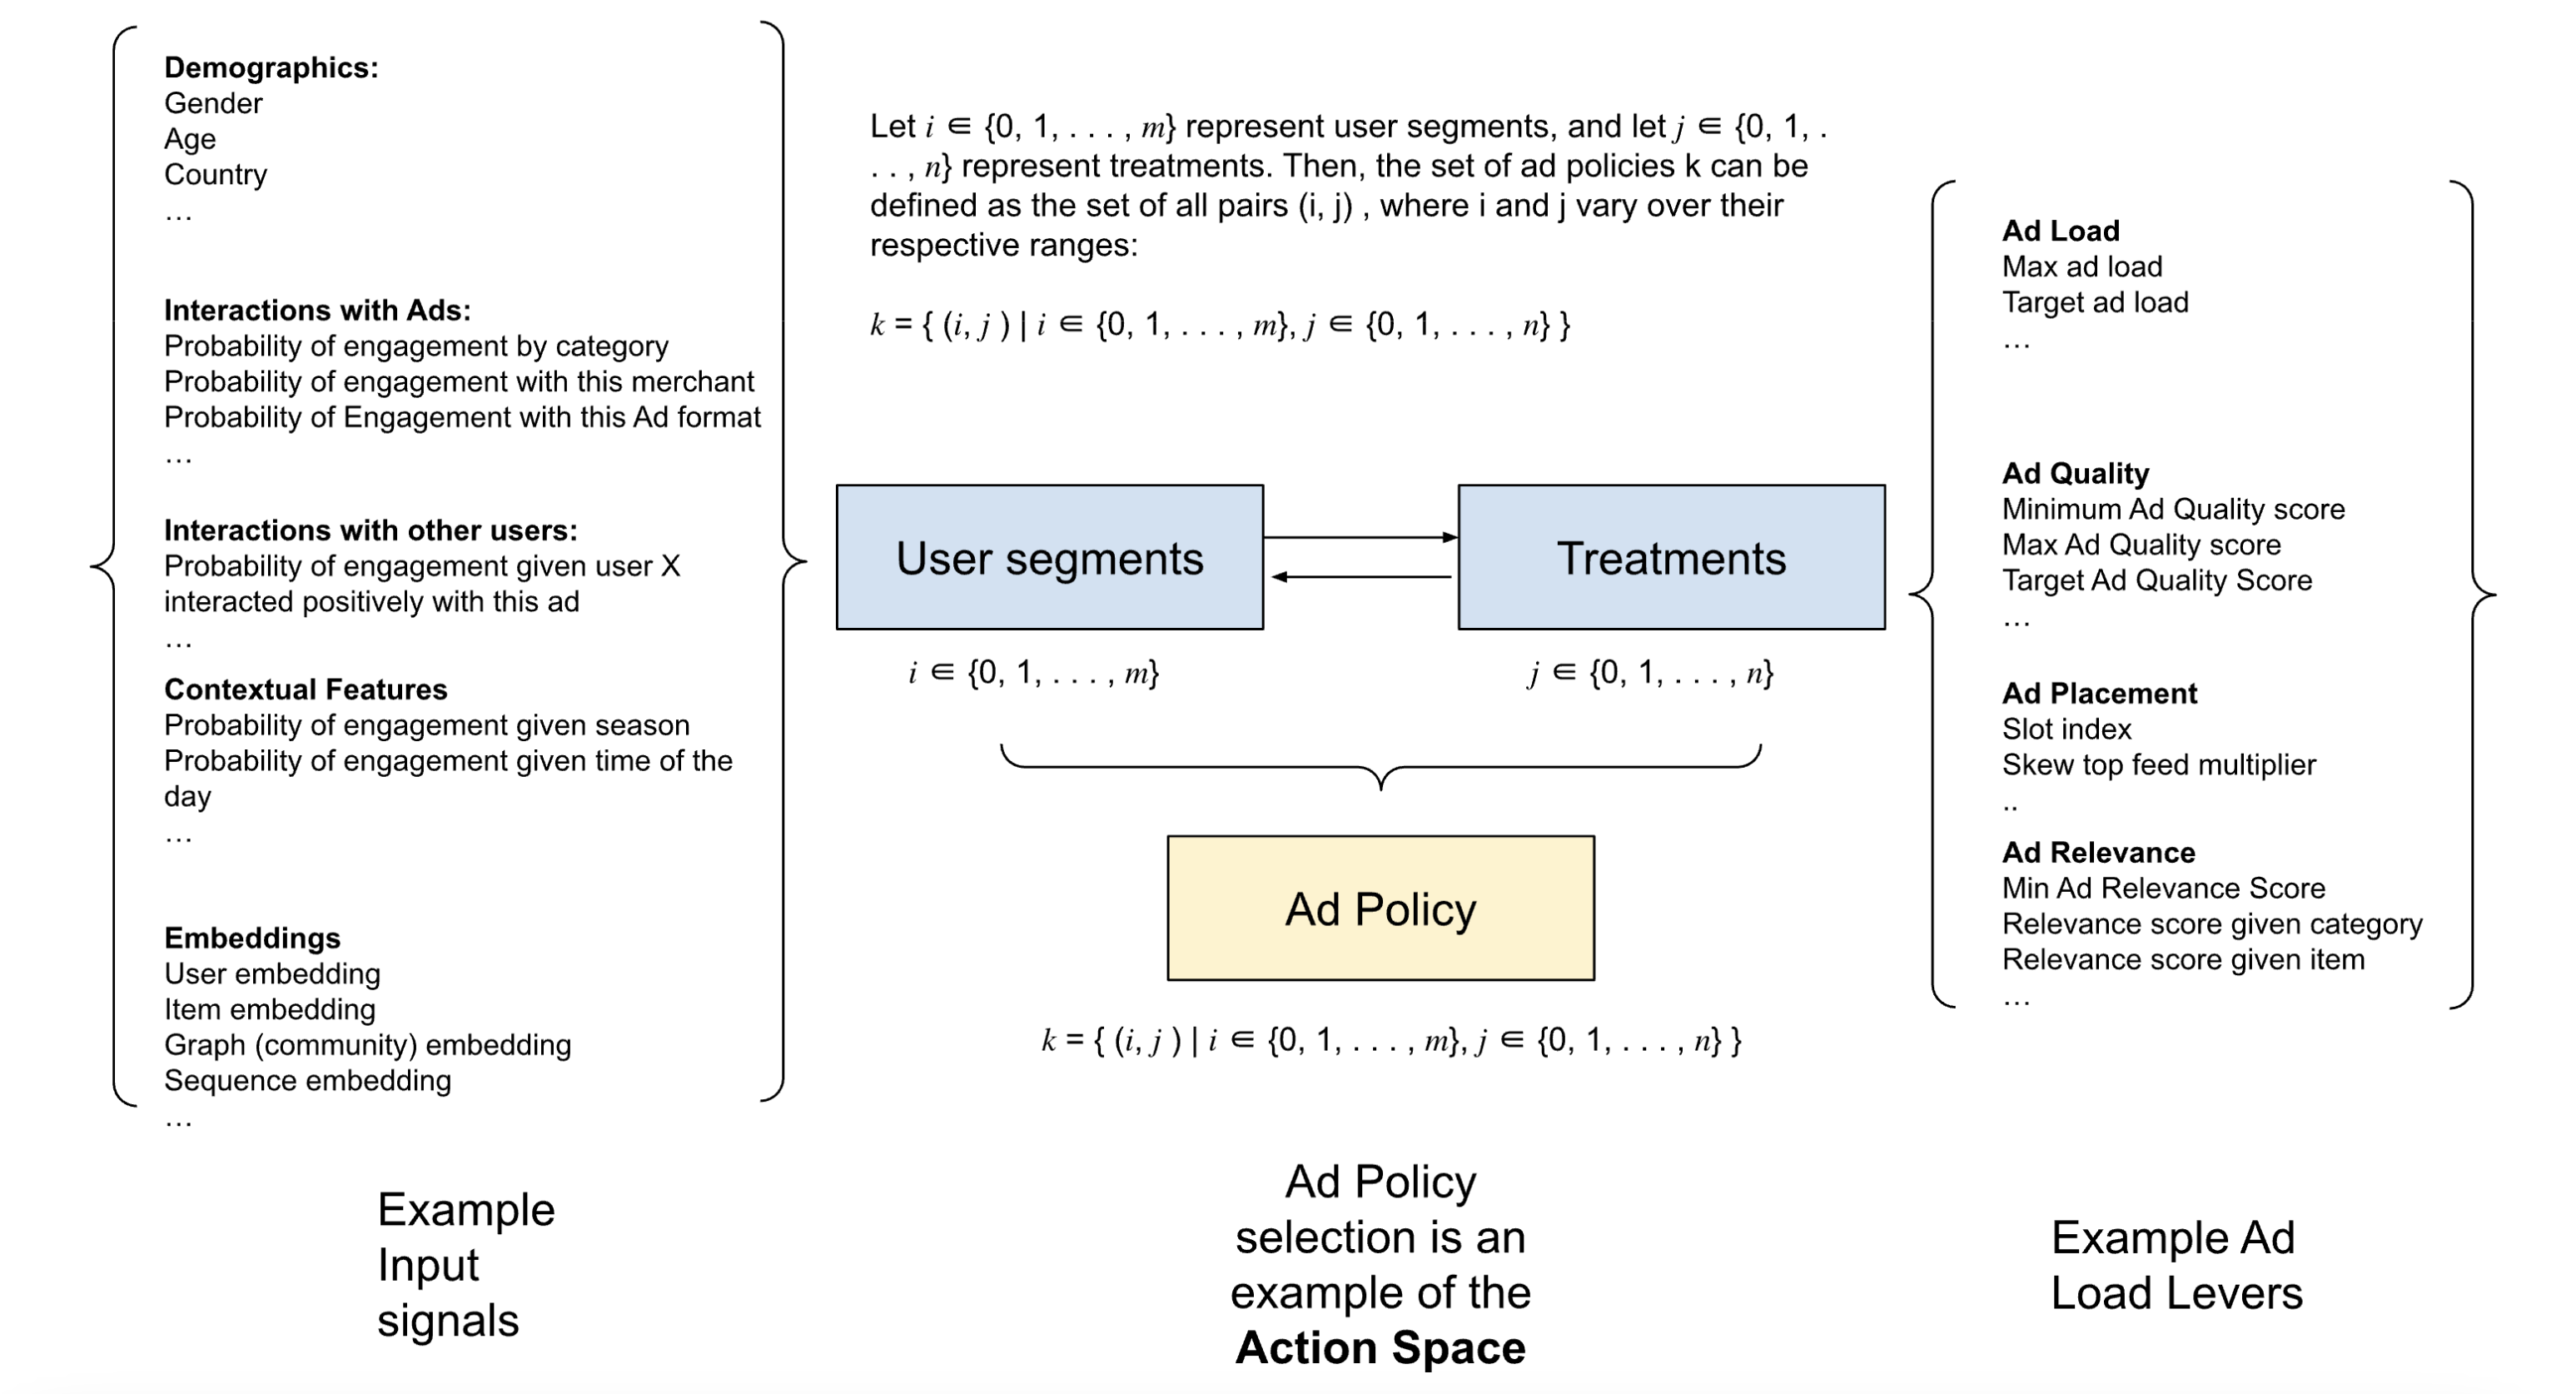
\includegraphics[width=\textwidth]{detailed_ad_policy.png}
    \caption{Example of an action set in the context of ad policies in recommendation systems}
    \label{fig:detailed_ad_policy}
\end{figure*}

\section{Conclusions}

The integration of RL in policy optimization for large-scale recommender systems has gained popularity as a promising approach to balance long-term and short-term objectives in environments with complex user behavior and revenue dynamics. However, scaling RL in practice presents challenges, including vast state and action spaces, reliance on proxy metrics, and significant computational demands. This paper provides an overview of effective, scalable techniques that address these challenges, offering insights into how RL can be applied at scale.
Unlike traditional methods that focus on optimizing short-term outcomes, RL’s cumulative reward framework enables it to account for both immediate and delayed feedback. Together, contextual bandits and offline replay offer scalable, interpretable solutions that approximate full RL while managing real-time constraints. Contextual bandits support selecting optimal actions within each interaction based on the current state, maximizing immediate rewards, which are typically proxy metrics of the true long-term reward. Offline replay complements this by enabling counterfactual learning: multiple treatments can be tested across randomized populations to evaluate causal effects, refining policies for diverse user segments.

Future research may focus on enhancing interpretability, refining reward functions, and exploring decentralized approaches to handle complex decision layers. These advancements will bring RL closer to fulfilling its potential in providing tailored, dynamic ad recommendations that align user satisfaction with business goals in large-scale recommendation systems.




\section*{Acknowledgements}
I would like to thank my advisor, Yuri Lawryshyn, for his valuable guidance and direction throughout this work. I also extend my gratitude to Adam Obeng, Bee-Chung Chen, and Jay Adams for their critical coaching and insights, which have significantly shaped my approach and understanding of industry practices. Their expertise has been key in aligning academic research with practical applications.

% This unnumbered section should be blank when submitting your paper. After review, you may include lists of people and organizations who supported the work.

% Print the biblography at the end. Keep this line after the main text of your paper, and before an appendix. 
% % THIS IS A LATEX TEMPLATE FILE FOR PAPERS INCLUDED IN THE
% *Anthology of Computers and the Humanities*. ADD THE OPTION
% 'final' WHEN CREATING THE FINAL VERSION OF THE PAPER. 
% DO NOT change the documentclass
%\documentclass[final]{anthology-ch} % for the final version
\documentclass[final]{anthology-ch}         % for the submission

% LOAD LaTeX PACKAGES
\usepackage{booktabs}
\usepackage{graphicx}
\usepackage{tabularx}
\usepackage{adjustbox}  % lets us make the table wider than \textwidth
\usepackage{setspace}
\usepackage{enumitem}
\usepackage{makecell}
% \usepackage{multirow}
\usepackage{float}

% \usepackage[table,xcdraw]{xcolor} % Allows the use of HTML colors

\addbibresource{bibliography.bib}


% \PassOptionsToPackage{table,xcdraw}{xcolor}


\geometry{
  a4paper,
  top=2cm,
  bottom=2cm,
  left=2cm,
  right=2cm
}

% ADD your own packages using \usepackage{}

% TITLE OF THE SUBMISSION
% Change this to the name of your submission
\title{A Review of Reinforcement Learning Applications in Ad Policy Optimization for Large-Scale Recommender Systems}

% AUTHOR AND AFFILIATION INFORMATION
% For each author, include a new call to the \author command, with
% the numbers in brackets indicating the associated affiliations 
% (next section) and ORCID-ID for each author.  
\author{Armando Ordorica}

\author{Yuri Lawryshyn}

% While we encourage including ORCID-IDs for all authors, you can
% include authors that do not have one by definining an empty ID.


% There should be one call to \affiliation for each affiliation of
% the authors. Multiple affiliations can be given to each author
% and an affiliation can be given to multiple authors. 
\affiliation{University of Toronto, Toronto, Canada}

% KEYWORDS
% Provide one or more keywords or key phrases seperated by commas
% using the following command

\keywords{Reinforcement Learning, Ad Policy Optimization, Contextual Bandits, Recommendation Systems,  Off-Policy Learning, Online Advertising, Deep Reinforcement Learning,  Multi-Objective Optimization}

% METADATA FOR THE PUBLICATION
% This will be filled in when the document is published; the values can
% be kept as their defaults when the file is submitted
\pubyear{2025}
\pubvolume{1}
\pagestart{1}
\pageend{1}
\conferencename{Proceedings of Conference XXX}
\conferenceeditors{Editor1 Editor2}
\doi{00000/00000}  

% \addbibresource{bibliography.bib}


\setstretch{2.0}

\begin{document}


\maketitle
% \doublespacing

\begin{abstract}
Balancing advertisements with organic content in large-scale recommendation engines is a well-known challenge in the industry. While ads are essential for revenue generation in platforms that integrate them alongside organic content, they often underperform in user engagement compared to organic content \cite{hochstein2023toward}. The key challenges in achieving this balance include ad selection, ranking, and integration with organic content. These involve decisions about whether to insert an ad, which ad to select, and where to place it \cite{zhao2020jointly}. Traditional methods optimize for the highest probability of ad clickthrough with fixed placements and are typically solved as supervised Machine Learning (ML) problems \cite{covington2016deep}. However, these approaches focus on optimizing single actions, overlooking the downstream impact of sequential user behavior and underutilizing valuable contextual signals. A more dynamic approach that accounts for context and optimizes the long-term value of action sequences, balancing both engagement and revenue, remains an open research area \cite{lin2023survey}.\\

Reinforcement Learning (RL) offers a promising framework to address the need for dynamic, context-aware optimization by formalizing the process of finding the best policy in sequential decision-making under uncertainty \cite{dimitrakakis2018decision}. However, implementing RL in large-scale recommendation systems faces challenges such as vast state and action spaces, the risk of poorly chosen reward functions, high computational costs \cite{pancha2022pinnerformer}, and the difficulty of interpreting online policy learning \cite{van2024practical}. This paper surveys existing methodologies and frameworks that utilize RL to enhance recommendation strategies, aiming to guide practitioners and researchers in navigating these challenges. Our analysis reveals that while fully online RL is powerful in theory, in practice, techniques like contextual bandits, offline replay, and surrogate reward modeling often yield more scalable and interpretable solutions for large-scale ad-serving.
\end{abstract}

% \tableofcontents

\section{Introduction}

Platforms such as Google, Meta, TikTok, and Pinterest offer content recommendation systems whose revenue models depend on an effective balance between advertisements and organic content \cite{zhao2020jointly} \cite{danescu2010competing}. This balance is essential to maximize immediate revenue while avoiding long-term issues such as ad fatigue, where users become less responsive to ads due to overexposure, and user churn, where users discontinue using the platform \cite{sagtani2023quantifying} \cite{silberstein2023combating}.\\

Over the past decade, deep learning has emerged as a promising technique that enables recommendation engines to better understand context through embeddings, significantly improving their ability to personalize content \cite{naumov2019deep} \cite{zhao2024survey}. However, deep learning approaches are often supervised and rely on measurable and observable short-term metrics used as model labels, such as the probability of a click-through or the likelihood of a video being watched in full \cite{nvidia_recommender_systems_2021}. Methodologies that use myopic objective functions to optimize these directly measurable short-term metrics often overlook the long-term value of a recommendation \cite{mazoure2021improving}. By focusing on immediate rewards, they may rank content based on short-term engagement metrics while neglecting the entire sequence of user interactions that involve delayed responses. Such approaches can result in suboptimal outcomes, such as promoting clickbait content that compromises long-term revenue and user engagement.\\

	% 4.	How does Reinforcement Learning (RL) offer a promising solution to these challenges?

To overcome the challenges of optimizing based solely on immediate objectives, Reinforcement Learning (RL), modeled as a Markov Decision Process (MDP), has emerged as a promising framework \cite{afsar2022reinforcement}. RL enables the consideration of long-term value by optimizing policies that maximize cumulative rewards over time, rather than focusing on short-term engagement metrics. In an MDP, actions are selected based on a policy ($\pi$), which chooses the action that maximizes the expected cumulative reward from the current state onward. This cumulative reward is typically conceptualized as the expected sum of future rewards, discounted over time using a discount factor. A lower discount factor places more emphasis on immediate rewards, effectively ignoring future outcomes. Conversely, a discount factor approaching one values future rewards more heavily, encouraging the policy to consider long-term benefits \cite{Sutton1998}. \\

In the context of recommendation systems, rewards can be defined to capture both user engagement and revenue objectives. Engagement rewards might include metrics such as time spent on the platform, content views, clicks, saves, shares, or likes \cite{wang2022surrogate}. Revenue rewards can be tied to ad-related metrics like ad impressions, ad clicks, conversions, or purchases resulting from ad exposure. These different rewards are often combined into a single utility function that reflects the platform’s overall objectives \cite{zhao2020jointly} \cite{zou2019reinforcement} \cite{xu2023optimizing}.\\

For example, the reward function  $r_t$  at time  $t$  can be defined as:

$$
r_t = \alpha \times \text{Engagement Metric}_t + \beta \times \text{Revenue Metric}_t,
$$ where  $\alpha$  and  $\beta$  are weighting factors that balance the importance of user engagement and monetization. By appropriately defining the utility function and choosing suitable weights, RL algorithms can optimize policies that enhance user experience while maximizing revenue over the long term \cite{zhao2020jointly, zhao2021dear, yan2020ads, sagtani2024ad}. \\


% What specific challenges are encountered when implementing RL in large-scale recommendation systems?
Despite the promising theoretical framework that RL offers for optimizing long-term value in recommendation systems, implementing RL in real-world, large-scale platforms remains complex \cite{dulac2021challenges}. First, in the context of recommendation systems, the state space, which reflects the current context of the user and the environment, and the action space, which captures how the recommender system can be tuned, are both essentially infinite \cite{zhu2021overview}. This vastness makes learning and optimization computationally intensive and difficult to discretize into individual actions and states, a critical requirement for policy learning \cite{afsar2022reinforcement} . \\ 

Second, designing appropriate reward functions is critical, as poorly chosen reward functions can lead to unintended system behaviors that degrade user experience or negatively affect business revenue \cite{everitt2021reward}. For example, a reward function that overly prioritizes click-based metrics may drive the system to promote clickbait content, boosting short-term engagement but eroding user trust and satisfaction over time \cite{wu2017returning}. Similarly, a reward function too heavily skewed toward revenue metrics could result in excessive ad load, disrupting the user experience and leading to churn. Striking the right balance in reward function design is essential to achieve both user engagement and monetization objectives without compromising the platform’s long-term goals.\\


Furthermore, interpretability is a major challenge in RL deployment. Understanding the learned policies--the strategies adopted by the RL agent--can be particularly difficult when policies are updated in real-time during user interactions (online policy learning) \cite{glanois2024survey} \cite{vouros2022explainable} \cite{dulac2019challenges}. This real-time adaptation complicates monitoring and evaluation, making it challenging to understand what is happening during online learning. In extreme cases, this lack of transparency could result in non-compliant or unethical behavior, posing significant risks to both users and the business \cite{lambert2023entangled}.\\

	% 7.	What are the objectives and contributions of this paper?
In light of the challenges outlined above, this paper examines methodologies and frameworks used to implement RL for large-scale recommendation systems, with a particular focus on contexts where ad revenue is central to the business model. Although previous surveys address RL in recommendation systems \cite{lin2023survey, afsar2022reinforcement}, they do not specifically explore how RL can balance the competing demands of ad and organic content. This paper fills that gap by analyzing approaches tailored to these unique challenges and bridging the divide between theoretical RL concepts and their real-world applications.
\\

The paper begins with a historical overview of ad selection and ranking systems, tracing the evolution from simple rule-based models and heuristic approaches to tree-based models and modern deep learning techniques. Each of these stages is explored in detail, highlighting their limitations and the motivations for adopting RL as the next paradigm in recommendation systems. Following this contextual history and motivation, the paper introduces key RL components such as the action space, state space, reward functions, and policies, using a straightforward toy example: the frozen lake problem. This example provides a foundation for understanding RL fundamentals, which are then mapped to real-world challenges in online advertising and recommendation systems. Drawing on these analogies, the paper offers a clear and practical framework to help practitioners navigate the implementation of RL and adapt these methodologies to their specific needs.


	% 8.	How will this paper help practitioners and researchers navigate the challenges of implementing RL in recommendation systems?


	% 13.	What is the structure of the paper, and what can readers expect in the subsequent sections?

\section{Paper Collection Methodology}

To ensure broad coverage, relevant papers were collected from both academic and industry sources. Foundational academic works such as \textit{Reinforcement Learning: An Introduction} \cite{Sutton1998}, \textit{Statistical Methods for Recommender Systems} \cite{agarwal2016statistical}, and \textit{Artificial Intelligence: A Modern Approach} \cite{russell2016artificial} were used to establish key mathematical foundations, including Markov Decision Processes (MDPs), Contextual Bandits, Off-Policy Learning, and Offline Replay.

To reflect the internal perspective of a production-facing ad policy team, a curated list of 10–15 papers referenced within Pinterest’s Ad Policy team was also compiled. Examples include \textit{Jointly Learning to Recommend and Advertise} \cite{zhao2020jointly}, \textit{DEAR: Deep Reinforcement Learning for Online Advertising Impressions in Recommender Systems} \cite{zhao2021dear}, \textit{Ad-load Balancing via Off-Policy Learning} \cite{sagtani2024ad}, and \textit{Practical Bandits} \cite{van2024practical}. In addition, targeted keyword searches such as “Reinforcement Learning ads [company name]” and “Contextual Bandit [company name]” were conducted for leading companies in the advertising and recommendation space (e.g., Google, Meta, Pinterest, Microsoft, TikTok, YouTube, LinkedIn),  surfacing additional papers describing real-world systems and methodologies. To complement those efforts, a separate search was conducted on Google Scholar for relevant review papers. While no surveys were found that specifically focused on RL in ad recommendation systems, related reviews on "contextual bandits", "ad fatigue", and "recommender systems" were used to identify additional references.

Finally, manual crawling of citation networks in cornerstone papers was used to identify additional key contributions. For instance, tracing citations from \textit{Jointly Learning to Recommend and Advertise} \cite{zhao2020jointly}, \textit{DEAR} \cite{zhao2021dear}, and \textit{Offline Reinforcement Learning} \cite{levine2020offline} led to works such as \textit{Ads Allocation in Feed via Constrained Optimization} \cite{yan2020ads} and \textit{A Contextual Bandit Bake-off} \cite{bietti2021contextual}.
In total, 153 papers were selected and reviewed. Papers were ranked according to three main criteria: influence, to capture the foundational or widely adopted ideas in the field; industry relevance, to ensure that the outcomes were sound, implementable, and actionable; and recency, to reflect the latest methodological developments and deployment practices.

While recent and highly cited work was prioritized, papers introducing novel methodologies were also included regardless of citation count. To contextualize the selected works, this survey builds from the ground up. Each component of the Markov Decision Process, including states, actions, rewards, and policies, is defined and illustrated using a toy example such as the Frozen Lake. This foundation is then extended to practice through a review of how each component is operationalized in industry, along with a discussion of the limitations of those approaches. Drawing on existing methods and lessons from industry, the resulting framework is intended to inform practitioners exploring how RL can be applied in their organizations to develop ad policies that balance monetization with organic engagement. A comparison between the toy example and real-world implementation parallels can be found in Table \ref{tab:comparison}.



\section{A Brief History of Ad Selection and Ranking in Recommendation Systems}

\begin{figure}[ht]
    \centering
    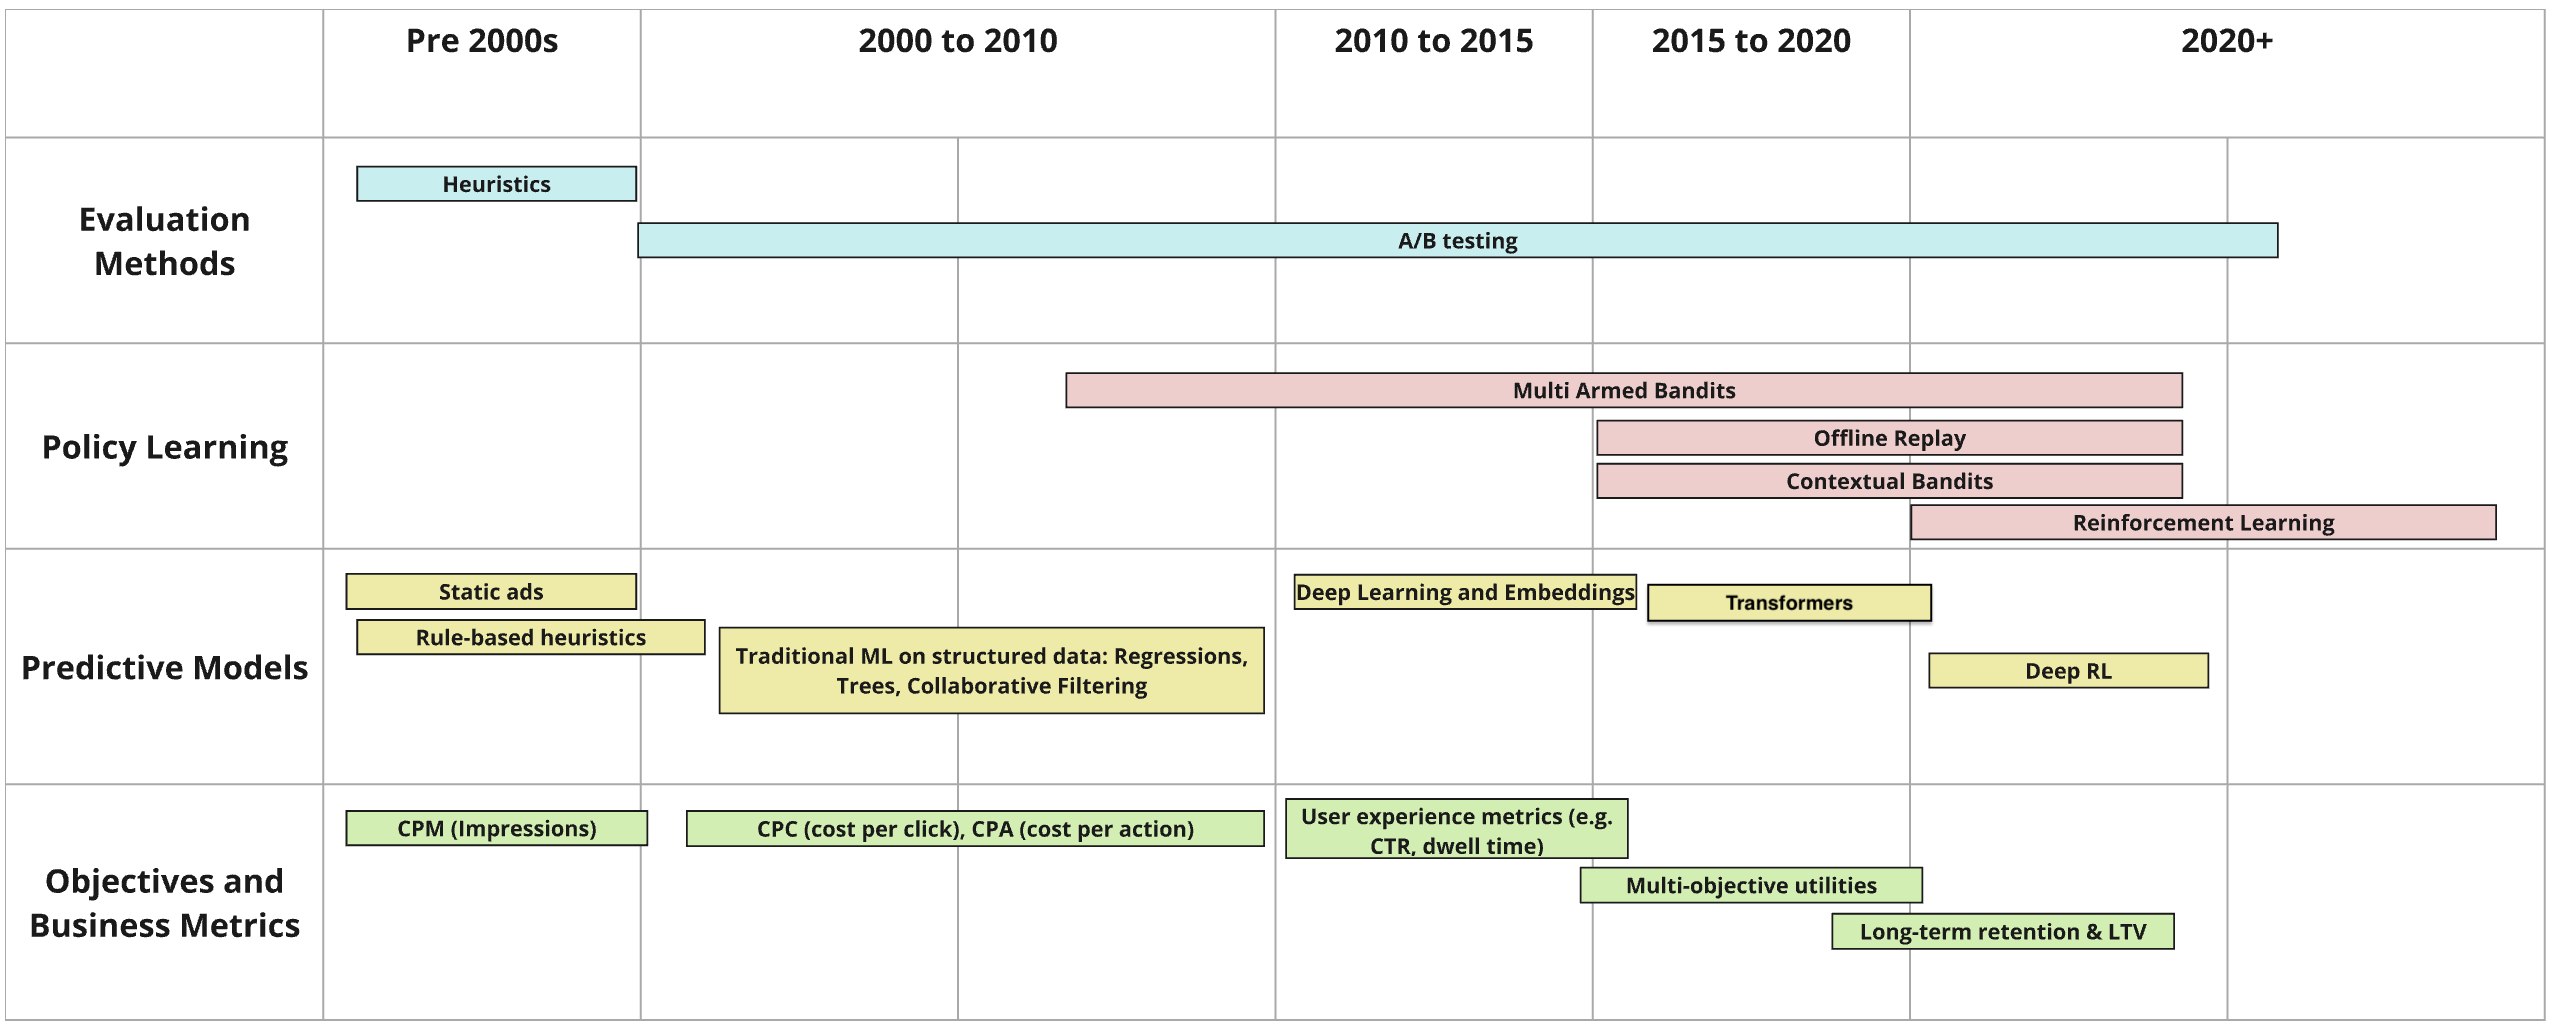
\includegraphics[width=\textwidth]{history_timeline_figure.png}
    \caption{Timeline Showing Initial Adoption and Popularization of Techniques and Methodologies in Online Advertising}
    \label{fig:ad_timeline}
    \vspace{0.2cm} % adds small vertical spacing
    \begin{flushleft}
        \footnotesize{\textit{Note:} The boundaries and lengths of rectangles are approximate. Innovations and transitions between techniques and objectives occurred gradually and continuously, rather than sharply at specific dates.}
    \end{flushleft}
\end{figure}


In online advertising, a good ad policy can result in positive revenue for the company while also boosting user experience. Conversely, a poor ad policy involves showing ads that are irrelevant to the user’s current intent, overloading the feed with excessive ad density, and failing to align content with the user’s interests. Irrelevant ad targeting can lead to ad fatigue, a state where users become desensitized or frustrated by excessive or poorly targeted ads, resulting in decreased engagement with both the ads and the platform as a whole \cite{ccelik2023ad}. \\

This section traces the evolution of advertising recommendation algorithms, culminating in the adoption of RL to overcome the limitations of earlier approaches. It begins by outlining how early online advertising primarily mirrored offline methods through banner ads and other static formats. It continues by explaining how static online advertising evolved over time to incorporate rule-based models and more sophisticated heuristic techniques. The discussion then transitions to the integration of machine learning methods, including regression-based models, tree-based algorithms, and collaborative filtering, followed by the emergence of deep learning and embedding-based approaches that effectively capture the nonlinear interactions between users and content. Finally, RL is introduced as a promising solution to address the shortcomings of preceding methodologies. This evolution is visually represented in Table \ref{fig:ad_timeline}, which shows the initial adoption and popularization of techniques and methodologies in online advertising. \\

\subsection{From Rule-Based Advertising to Traditional Machine Learning}
\textbf{Around the early 2000s, online advertising largely mirrored offline practices, heavily relying on non-targeted formats such as banner ads \cite{kant2021history}.} These generic advertising methods conflicted with the objective of search engines of efficiently directing users to relevant content \cite{fain2006sponsored}. As a marginal improvement on nontargeted ad formats like banner ads, advertisers began to utilize simple \texttt{if-then} logic with predefined rules to select and display ads based on basic criteria like user demographics. While rule-based systems were straightforward to implement, their lack of flexibility and personalization became evident as ad fatigue, defined as reduced user engagement due to repeated exposure to the same advertisement, persisted \cite{abrams2007personalized}. This issue underscored the necessity of not only leveraging user signals but also optimizing ad load tuning parameters, such as frequency and placement, to maintain user interest and maximize click-through rates \cite{abrams2007personalized}. For instance, researchers at LinkedIn introduced concepts like top slot - highest eligible position for an ad within the feed -  and minimum gap - the required distance between consecutive ads to prevent oversaturation - as ad load tuning parameters \cite{yan2020ads}. Their research indicated that users are more likely to click on ads that are spaced farther apart \cite{yan2020ads}. \\

\textbf{The evolution of ad pricing, from paying for impressions to paying for user actions, created pressure within the online advertising industry to improve relevance and performance-based metrics \cite{hu2004performance}.} Sponsored search, introduced by GoTo (later Overture), allowed advertisers to bid on specific keywords, directly linking ads to user queries and addressing the limitations of generic advertising  \cite{fain2006sponsored}. Foundational pricing models, such as Cost per Mille (CPM), charged advertisers per 1,000 impressions and closely mirrored offline practices \cite{wikipedia-cpm}. Yahoo!, through the acquisition of Overture \cite{wsj2003yahoooverture}, later introduced Cost per Click (CPC) \cite{ellam2003overture}, a performance-based pricing model that shifted costs to reflect measurable user engagement. This evolution continued with the introduction of Cost per Action (CPA), which tied fees to specific user actions beyond clicks, such as purchases or sign-ups. These changes incentivized the advertising industry to innovate, leading to the development of more relevance-focused strategies. These foundational pricing models remain integral to the utility functions that underpin contemporary ranking algorithms \cite{fain2006sponsored}. As advertisers increasingly demanded performance-based pricing, the ad tech industry was compelled to innovate within a competitive yet lucrative market, addressing the limitations of rule-based and heuristic models through the adoption of machine learning techniques to enable more dynamic and data-driven approaches \cite{zhang2018whole}.



\textbf{The next set of innovations following heuristics and performance-based targeting was led by machine learning (ML) and A/B testing \cite{barajas2022online}}. From 2010 to 2015, ad selection techniques evolved significantly with the adoption of machine learning models such as Logistic Regression, Decision Trees, and Gradient Boosting Machines \cite{cui2015global}. By leveraging historical data and diverse user behavior signals, these models enabled more accurate predictions of user engagement \cite{cui2015global}. In parallel, A/B testing allowed practitioners to systematically compare models and features, ensuring that any new implementation delivered measurable performance gains \cite{barajas2022online}.
Despite these successes, traditional tabular models struggled to capture nuanced user intent, particularly when processing more complex data such as images or text. In the early 2010s, deep learning gained momentum with breakthroughs like AlexNet \cite{krizhevsky2012imagenet}, which demonstrated the power of neural networks to handle unstructured high-dimensional data. This ability to capture complex, nonlinear interactions dramatically improved ad recommendations, especially through the use of embeddings, which are dense vector representations that map words or images into high-dimensional spaces. Metrics like cosine similarity further refined personalization by aligning recommendations with user interests \cite{covington2016deep}. Embedding-based models, particularly two-tower architectures, presented a major leap forward in ad recommendation systems by effectively capturing intricate relationships between users and ads. These models utilize two neural networks: one dedicated to encoding user information and the other to encoding ad (item) information. The outputs from these networks are then combined to predict user engagement with ads \cite{vorotilov2023scaling}. This approach not only boosted accuracy but also scaled effectively. Despite the significant improvements that embedding-based models introduced in terms of predictive accuracy and scalability of ad recommendation systems, the practical challenges of balancing multiple objectives, such as maximizing revenue, mitigating ad fatigue, and sustaining long-term user engagement remained unresolved.  


\textbf{Multi-Armed Bandits (MABs) emerged as a powerful method for online advertising around the 2010s to minimize user exposure to suboptimal ad configurations, effectively tackling the explore–exploit tradeoff, which consists of finding the optimal balance between choosing new ad policies with unknown performance and showing older ad policies with known positive performance \cite{schwartz2017customer} \cite{burtini2015improving}.} MABs are a class of algorithms for dynamic decision-making under uncertainty, originally developed in mid-20th-century probability theory \cite{robbins1952sequential}. While MABs had been widely applied in areas such as clinical trials \cite{villar2015multi} \cite{thompson1933likelihood}, they only gained significant traction in online advertising around the 2010s \cite{schwartz2017customer}.  

MABs allow platforms to reduce unnecessary exposure to a suboptimal treatment by continuously updating the probability distribution of which treatment is most likely to yield the highest reward \cite{kuleshov2014algorithms}. In clinical trials, for instance, a bandit algorithm reduces unnecessary exposure to suboptimal treatments by updating its reward estimates in real time: it allocates more patients to the better-performing treatment (exploitation) while still testing others that could be better (exploration) \cite{kuleshov2014algorithms}\cite{villar2015multi}. In this setting, the “reward” might be a measurable improvement in patient health or recovery time \cite{villar2015multi}. The same principle applies to online advertising, where “treatments” translate into specific ad configurations, defined by parameters such as displacement cost, reserve price, ad load, and ad placement. “Rewards” in online advertising typically represent user engagement metrics such as clicks or conversions \cite{schwartz2017customer}. Advertising platforms should continuously “explore” new treatments to test new ads, formats, and targeting strategies to avoid stagnation, while simultaneously “exploit” existing high-performing treatments to ensure near-term revenue targets are met \cite{schwartz2017customer}.  

In contrast to traditional A/B tests, where there are randomized treatments assigned for a predetermined amount of time, MABs dynamically learn which configuration yields the highest reward for each user at a particular time. This approach reduces the time users are exposed to suboptimal ad configurations, thereby mitigating losses in engagement and long-term revenue \cite{schwartz2017customer}. Although this dynamic learning framework effectively tackles the explore–exploit tradeoff, defining the precise set of rewards and objectives to optimize remains an open challenge, particularly when advertisers must juggle multiple goals such as revenue and long-term user satisfaction \cite{wen2019learning}.

\textbf{To address this need for clear, multi-objective definitions, such as balancing user satisfaction and revenue, utility functions have been employed in online advertising since the early 2000s \cite{engel2008incorporating}.} Rooted in microeconomic theory dating back to the mid-20th century, utility functions are mathematical constructs that quantify preferences and the net value of conflicting objectives \cite{Stigler1950} \cite{vonNeumannMorgenstern1944}. Introduced to formalize decision-making under uncertainty, they model and quantify consumer preferences, enabling advertisers and publishers to encode multiple objectives, such as revenue, user satisfaction, and long-term platform health, into a single or composite utility metric \cite{engel2008incorporating}. By integrating utility functions into MAB-based frameworks, advertisers can systematically guide the exploration–exploitation process toward a unified reward signal that balances short-term performance (e.g., clicks, impressions, or conversions) with long-term considerations (e.g., minimizing ad fatigue or maintaining user trust). This approach allows for principled trade-offs, optimizing for immediate gains while safeguarding long-term engagement.


\subsection{Advances in Deep Learning: Attention Models, Transformers, and Contextual Bandits}

\textbf{While embedding-based models greatly enhanced the predictive power of recommendation systems, capturing the full complexity of user sequences, especially over long time spans, remained a challenge for sequential deep learning methods such as  Long Short-Term Memory networks (LSTMs) and Gated Recurrent Units (GRUs) \cite{vaswani2017attention} \cite{gao2024mamba}.} Traditional recurrent networks (e.g., LSTMs or GRUs) process sequences step by step, typically encoding an entire sequence into a single fixed-size vector \cite{Sutskever2014}. This design poses several challenges. Because Recurrent Neural Networks (RNNs) operate strictly in a sequential manner, they cannot process multiple parts of the sequence in parallel, creating bottlenecks and risking the loss or blurring of details, especially those from earlier steps in long sequences \cite{vaswani2017attention}.  Moreover, standard RNNs inherently prioritize recent inputs as information is passed along, which attenuates earlier signals and leads to the well-known vanishing gradient problem in lengthy sequences and fails to effectively capture long-term dependencies \cite{Bengio1994}\cite{Pascanu2013}. 


\textbf{To address training inefficiencies in RNNs and the difficulty of capturing long-term dependencies, attention mechanisms allow direct access to any position in the sequence, enabling the model to focus on relevant features in the sequence regardless of their temporal distance \cite{vaswani2017attention}. }By computing pairwise interactions across all positions in the sequence, Transformers overcome the sequential bottlenecks of RNNs and enable parallel computation \cite{vaswani2017attention}.  This mechanism also allows the model to incorporate contextual signals, such as user demographics, session-level metadata, or item attributes, at any point in the sequence, rather than strictly depending on a running hidden state \cite{kang2018sasrec}. The ability to attend to any part of the input at any time allows Transformers to model long-range dependencies with far greater efficiency and accuracy than RNN-based architectures \cite{vaswani2017attention}. This paradigm shift led to the development of the Transformer architecture, which entirely replaces recurrence with self-attention, fundamentally redefining sequence modeling \cite{vaswani2017attention}.

\textbf{The Transformer’s parallel attention architecture is a natural fit for modern hardware.} Since self-attention and feed-forward layers are implemented with large matrix operations, the model makes efficient use of Graphics Processing Units (GPUs) and Tensor Processing Units (TPUs), which excel at parallel computation \cite{vaswani2017attention}. Unlike RNNs that left many GPU cores underutilized due to their step-by-step nature, Transformers keep the hardware busy by processing many elements concurrently. This yields significantly shorter training times compared to earlier recurrent models. Moreover, Transformers scale up seamlessly: training can be distributed across multiple GPUs, and larger batches or longer sequences can be handled without a drop in throughput \cite{shim2022comparison}. Engineers can simply add more GPU workers to accommodate bigger models or more data, achieving near-linear speedups in many cases \cite{brown2020language}. The ability to train deep models efficiently at scale has unlocked previously impractical projects, and Transformer-based architectures (e.g. BERT, GPT) are now standard building blocks in modern AI systems \cite{brown2020language} \cite{kaplan2020scaling}. One of the key innovations of the Transformer architecture is its multi-head attention mechanism \cite{vaswani2017attention}. Instead of relying on a single attention distribution, multiple attention “heads” are trained in parallel, each with its own set of learned parameters. This design allows the model to capture a range of relationships or patterns within the same sequence \cite{vaswani2017attention}.In practice, each head can focus on different aspects. One head might emphasize local dependencies in the user’s interaction history, while another one might highlight more global, long-range correlations \cite{vaswani2017attention}.


\textbf{In an advertising context, multi-head attention naturally accommodates multi-objective learning \cite{ma2018modeling}.} For example, one head could be tuned to prioritize short-term engagement metrics (e.g., click-through rate or CTR) by attending to recent user activities and relevant ad features, while another head could emphasize longer-term outcomes, such as mitigating ad fatigue or preserving user satisfaction \cite{zhao2019recommending} \cite{ma2018modeling}. Each head learns a distinct set of attention weights, enabling the model to isolate and capture unique signals that serve different goals \cite{an2024tmh}. The outputs from these multiple heads are then aggregated, typically concatenated and linearly transformed, into a single representation or score, providing a unified but multi-faceted embedding of user–ad interactions \cite{vaswani2017attention} \cite{lyu2023entire}. However, determining the appropriate attention heads and their optimal weighting remains a complex challenge \cite{vaswani2017attention}\cite{Kang2018} \cite{Voita2019}. The optimal weights may vary not only across different users and content types but also over time \cite{Zhou2018} \cite{Zhou2019}. Additionally, shifting business objectives, engineering constraints, and competing optimization objectives further complicate the design process \cite{Mehrotra2018} \cite{Mehrotra2020} \cite{Jannach2023}. 

%How is head selection and weighing typically done 
\textbf{Selecting the right heads in Multi-Task Attention Models and determining their optimal weighting is not a deterministic process \cite{Michel2019} \cite{Voita2019}.} It typically requires iterative experimentation, involving both offline analysis (e.g., hyperparameter tuning, head ablation studies) and online testing (A/B experiments) \cite{Michel2019} \cite{kang2018sasrec}. This process is particularly challenging for new users and new content, where slow adaptation can result in suboptimal personalization and early churn \cite{Schein2002, Bobadilla2013}. 

%tie this up to Offline Replay 
\textbf{To address difficulties related to policy optimization - like weight tuning and head selection - \textit{Offline Replay} is often employed to find optimal policies in large parameter search spaces  \cite{agarwal2016statistical} \cite{levine2020offline} \cite{agarwal2020optimistic}.} This technique typically begins with data collection via A/B/n experiments, where different policies are randomly assigned to users \cite{agarwal2019online} \cite{chen2009large}. Afterward, Offline Replay simulates the effects of various ad policies across different user segments and estimates the potential rewards based on logged interactions \cite{agarwal2016statistical}. In this context, “reward” refers to the performance metric we aim to maximize (i.e. clicks, likes, shares, revenue) \cite{wu2017returning}. However, in many cases, the true optimal treatment is not explicitly tested \cite{agarwal2019online}. Here, importance sampling corrects for differences between the observed behavior policy and the target policy, improving estimation accuracy \cite{Sutton1998} \cite{dudik2011doubly}.  Based on the collected data on random assignments between policies and users typically involved in Offline Replay, one can use different policy learning methods to map the optimal policies from user ids, content types, and other contextual signals for the optimal weights at any point in time \cite{swaminathan2015counterfactual}. 


%  As a form of counterfactual learning, it estimates potential rewards under different policies by simulating outcomes based on logged interactions. This enables the system to learn from sparse or delayed feedback and serves as a critical tool for safely testing new policies offline \cite{sagtani2024ad}.\\

% In this context, “reward” refers to the performance metric we aim to maximize. For example, a click or any other positive action on an item is considered a reward. Sometimes, a positive action like a click can be weighted by a downstream utility, such as advertising revenue or time spent on a landing page (the page displayed after a user clicks on a recommended item), to derive a weighted reward. Our goal is to estimate the expected reward of a new ad policy using data collected in the past \cite{agarwal2016statistical}.\\

\textbf{Offline replay  often assumes that user preferences and item availability do not change significantly during data collection. }However, in real ad systems, these factors can shift, causing offline data to become stale or biased \cite{levine2020offline} \cite{agarwal2014taming}. Contextual bandits address this limitation by leveraging continuous feedback from live user interactions, preventing the policy from being locked into a static offline dataset \cite{li2010contextual}. Contextual bandits can be thought of as a special case of RL, where an action selection does not influence future states \cite{bubeck2012regret} \cite{Sutton1998}. Unlike full RL, which models long-term state transitions, contextual bandits assume that each decision is independent, optimizing for immediate rewards rather than a multi-step trajectory \cite{bubeck2012regret} \cite{Sutton1998}. This makes them particularly well-suited for recommender systems, where ranking decisions can be treated as independent events \cite{afsar2022reinforcement} \cite{zhou2016latent}. Additionally, contextual bandits naturally balance exploration and exploitation, allowing them to adapt dynamically to user behavior in real time \cite{li2010contextual}. However, a practical limitation of contextual bandits is that they select actions from a fixed set defined at deployment time, such as preconfigured ad policies or treatment arms \cite{bietti2021contextual}. As a result, the policy’s performance is inherently constrained by the quality and granularity of the available states and actions at the time of inference \cite{dimitrakakis2018decision}.

\textbf{Although contextual bandits inherently focus on short-term rewards, they can be tuned to approximate long-term objectives by encoding historical or delayed outcomes into the feature space or the immediate reward function \cite{mcdonald2023impatient} \cite{wu2017returning}.} For instance, if an attention head emphasizing ad engagement indirectly correlates with better retention, a contextual bandit can increase its weight over time, provided that retention signals are reflected in the contextual features or the reward proxy \cite{yi2023progressive}. However, full RL remains more appropriate for scenarios demanding explicit multi-step optimization, where actions taken now significantly shape future user states \cite{gauci2018horizon}. Contextual bandits thus offer a practical trade-off, providing continuous adaptation and efficient online learning without the computational complexity of fully modeling multi-step state transitions \cite{gauci2018horizon} \cite{levine2020offline}.


\textbf{Despite the practical advantages that contextual bandits offer for real-time experimentation and short-horizon reward maximization, they remain limited in scenarios where user states evolve over repeated interactions \cite{Sutton1998}.} Modern advertising platforms often contend with extended user sessions and multiple recurring visits, demanding an approach capable of modeling multi-step feedback loops. RL naturally extends these capabilities by incorporating stateful dynamics and cumulative rewards, capturing phenomena like ad fatigue \cite{ccelik2023ad} and long-term retention \cite{wu2017returning}. Recent industrial deployments underscore RL’s growing importance in ads: ByteDance uses RL-based systems \cite{zhao2020jointly,zhao2021dear} to balance immediate revenue with session-level engagement in short-video feeds, Meta (Facebook) has leveraged policy-gradient methods for sequencing notifications and ad placements over evolving user states \cite{gauci2018horizon}, and companies like Google are experimenting with RL-driven ad scheduling that accounts for shifting user contexts at scale \cite{zhao2024survey}. These efforts demonstrate how RL can transcend the myopic focus of bandits to address long-horizon outcomes, multi-objective trade-offs, and dynamic user behaviors. In the sections that follow, we explore how these RL paradigms are integrated into large-scale advertising stacks, focusing on core algorithms, design decisions, and lessons learned from real-world implementations.



\section{The RL formulation of the Ad Recommendation Problem}

In RL, the \textbf{GridWorld problem }is a foundational example of a Markov Decision Process (MDP), where an \textbf{agent} interacts with a \textbf{deterministic environment} by performing \textbf{discrete actions}, such as moving up, down, left, or right, to navigate through a grid with the objective of reaching a goal, while potentially avoiding obstacles or hazards. A more complex variant is the \textbf{FrozenLake problem}, which features a \textbf{stochastic environment} where movements are uncertain due to a slippery surface (\textcolor[HTML]{1E90FF}{F}) as shown in Figure~\ref{tab:frozen_lake} \cite{FrozenLakeGymnasium2023}. Here, \textbf{actions do not always lead to the intended next state}, adding complexity by requiring policies that effectively manage uncertainty. In this paper, \textbf{we use the FrozenLake problem as a representative framework for stochastic environments and leverage this template to describe the ad optimization problem as an RL task}. Specifically, we will explore components of the underlying MDP, such as states, actions, and rewards, and investigate key RL concepts including policy evaluation, value iteration, and policy iteration. The grid is typically represented as shown in Figure~\ref{tab:frozen_lake}:


\label{frozen_lake}


\begin{figure}[ht]
\centering
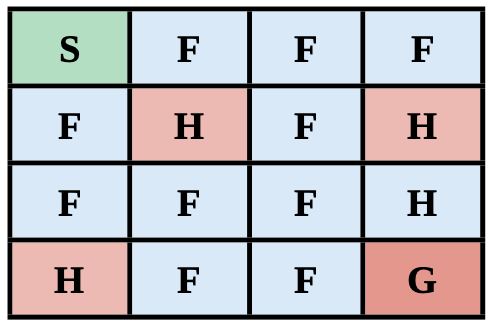
\includegraphics[width=0.35\linewidth]{frozenlake-table.png}
\caption{Frozen Lake Environment Grid}
\label{tab:frozen_lake}
\end{figure}


% \begin{table}[ht]
%     \centering
%     \setlength{\arrayrulewidth}{0.5mm}
%     \setlength{\tabcolsep}{12pt}
%     \renewcommand{\arraystretch}{1.5}
%     \begin{tabular}{|c|c|c|c|}
%         \hline
%         \cellcolor[HTML]{A9DFBF}\textbf{S} & \cellcolor[HTML]{D6EAF8}\textbf{F} & \cellcolor[HTML]{D6EAF8}\textbf{F} & \cellcolor[HTML]{D6EAF8}\textbf{F} \\ \hline
%         \cellcolor[HTML]{D6EAF8}\textbf{F} & \cellcolor[HTML]{F5B7B1}\textbf{H} & \cellcolor[HTML]{D6EAF8}\textbf{F} & \cellcolor[HTML]{F5B7B1}\textbf{H} \\ \hline
%         \cellcolor[HTML]{D6EAF8}\textbf{F} & \cellcolor[HTML]{D6EAF8}\textbf{F} & \cellcolor[HTML]{D6EAF8}\textbf{F} & \cellcolor[HTML]{D6EAF8}\textbf{H} \\ \hline
%         \cellcolor[HTML]{F5B7B1}\textbf{H} & \cellcolor[HTML]{D6EAF8}\textbf{F} & \cellcolor[HTML]{D6EAF8}\textbf{F} & \cellcolor[HTML]{F1948A}\textbf{G} \\ \hline
%     \end{tabular}
%     \caption{Frozen Lake Environment Grid}
%     \label{tab:frozen_lake} % This label is used to reference the table
% \end{table}


\begin{table*}[ht]
    \centering
    \small
    \begin{tabular}{|>{\centering\arraybackslash}p{3cm}|p{3.5cm}|p{9cm}|}
        \hline
        \textbf{Component of Markov Decision Process Formulation} & \textbf{Frozen Lake Example} & \textbf{Large Scale Recommendation Systems for Ad Policy Optimization} \\ 
        \hline
        \textbf{Environment} & The frozen lake. & The users. \\ 
        \hline
        \textbf{Goal} & Reach the goal (G) from the start position (S) while avoiding holes (H). The agent must avoid falling into a hole, and reaching the goal faster is rewarded. & Maximize revenue without compromising user experience. \\ 
         \hline
          \textbf{Episode} & A game. & A time period (T), typically 2 weeks, corresponding to an A/B experiment where enough data is collected to evaluate policy performance across users. \\ 
        \hline
        \textbf{Rewards} & Rewarded for reaching the goal (i.e., +100), but penalized for delays (i.e., -1 per step). & 
        The reward is typically represented by a utility function, which could be a weighted sum of metrics like user engagement (clicks, time spent) and revenue generated (ad clicks, conversions). The challenge lies in balancing short-term revenue with long-term user retention. \\ 
        \hline
        \textbf{Agent} & The learner. & The Recommendation System. \\ 
        \hline
        \textbf{Actions} & Up, down, left and right. & 
        Basically infinite. But when it comes to ad recommendations specifically, some typical actions are the following: 
        \begin{itemize}
            \item Reserve Price Floor: The minimum price at which an ad impression is sold.
            \item Displacement Cost Threshold: A measure of the opportunity cost for showing an ad.
            \item Max Ad Load: The maximum number of ads that can be shown without reducing user satisfaction.
            \item Ad Quality Thresholds: Standards used to ensure ads meet a quality bar before being shown.
            \item Ad Placement: The specific position of ads within the user feed (e.g., first, third, or fifth position).
        \end{itemize} \\
        \hline
        \textbf{States} & All possible grid positions the agent can occupy, representing the state space of the environment. & 
        \textbf{Signals}:
        \begin{itemize}
            \item User Context: Demographics, user profile
            \item Interaction Data: Previous interactions with ads, organic content
            \item Contextual Features: Time of day, browsing context
            \item Embeddings: Latent feature representations of user interests or ad features
        \end{itemize} \\
        \hline
        \textbf{Policy} & A mapping of grid positions to optimal action to take for a maximum reward. & 
        A mapping of user segments to ad treatments to maximize both revenue and user experience. This policy can be dynamically adjusted based on real-time feedback or offline simulations. \\ 
        \hline
    \end{tabular}
    \caption{Comparison of Frozen Lake Example and Large-Scale Recommendation Systems for Ad Policy Optimization}
    \label{tab:comparison}
\end{table*}

\subsection{The Agent and its Objective}
While toy examples like GridWorld \cite{Sutton1998}  and Frozen Lake \cite{frozenlake} provide well-defined, relatively simple environments where RL algorithms can be easily tested, transitioning these insights to real-world recommendation systems is far more complex due to factors like vast state–action spaces and delayed rewards, and environment observability \cite{dulac2019challenges, kaelbling1996reinforcement}. \textbf{Observability refers to the degree to which an agent can directly perceive the complete state of the environment} \cite{kaelbling1998planning}. In fully observable settings (such as the FrozenLake), the agent sees the true state at every step, enabling straightforward decision-making \cite{kaelbling1998planning}. However, real-world environments, including \textbf{recommendation systems, are often partially observable \cite{lu2016partially}}; the agent must infer the underlying state from incomplete or noisy signals, increasing both the computational complexity of learning and the uncertainty of policy outcomes \cite{wu2021partially}. In the FrozenLake environment, the \textbf{agent is a decision-maker that observes its surroundings and chooses actions}. It learns to navigate the grid to reach the goal (\textcolor[HTML]{FF4500}{G}) from the start position (\textcolor[HTML]{228B22}{S}) while avoiding holes (\textcolor[HTML]{FF0000}{H}) and navigating slippery surfaces (\textcolor[HTML]{1E90FF}{F}). By analogy, in ad policy optimization, \textbf{the agent is the algorithm responsible for serving ads}, which must balance two primary \textbf{objectives}: maximizing revenue while maintaining (or ideally enhancing) user engagement \cite{Theocharous-2015, zou2019reinforcement}. Ultimately, both the FrozenLake agent and the ad-serving algorithm share the same high-level goal: to maximize long-term rewards through strategic actions grounded in observed states.

The use of a \textbf{reward signal} to formalize the idea of a goal is a distinctive feature of RL \cite{Sutton1998}. In an MDP, the reward is a scalar value the agent receives after taking an action in a given state and transitioning to a new state, serving as immediate feedback on the benefit or cost of the action \cite{kaelbling1996reinforcement}. This feedback allows the agent to learn a policy that maximizes the cumulative reward over time \cite{kaelbling1996reinforcement}. In simple RL scenarios, rewards are typically straightforward. For instance, the agent might receive -1 per move (to encourage shorter paths), +100 for reaching the goal (G), and -100 if it falls into a hole (H), ending the episode. \textbf{However, in real-world recommendation systems, reward structures can be far more nuanced.  It is often unclear which user behaviors warrant the highest reward or how to weigh different signals} \cite{mcdonald2023spotify}. In online advertising, for example, low-intent actions such as clicks may be valued less than high-intent actions like saves or purchases. Moreover, deciding how to balance these varied signals in a single reward function can be both subjective and complex, especially when multiple objectives (e.g., revenue, user satisfaction, and content diversity) must be optimized \cite{mcdonald2023spotify}.\\

Ad recommendation engines often need to \textbf{balance multiple objectives}, such as maximizing user engagement while also ensuring ad revenue \cite{zhang2018whole, yan2020ads, sagtani2024ad}. Long-term engagement and revenue are metrics that are particularly difficult to measure directly, especially in randomized controlled experiments that typically span only a couple of weeks \cite{mcdonald2023spotify}. The delay in outcomes (e.g., retention signals may take months to manifest) and the often subtle impact of a single intervention can make it nearly impossible to detect meaningful changes within such short time frames \cite{mcdonald2023spotify}.  As a result, proxy metrics are commonly used. For instance, click-through rate (CTR) and ad impressions serve as approximate measures of revenue, while session duration, saves, and shares act as proxies for longer-term engagement \cite{wang2022surrogate}. However, these simpler proxies can fail to capture the system’s true long-term objectives, occasionally leading to suboptimal policies \cite{mazoure2021improving}. A high CTR may reflect short-term engagement, yet it can ultimately induce ad fatigue or frustrate users if the ads are misaligned with their actual interests \cite{hohnhold2015focusing, sagtani2024ad}. Table \ref{fig:proxy-metrics} summarizes some of the most commonly used proxies in the industry across dimensions of revenue, engagement, and ad fatigue. 


% \begin{figure}[H]
% \centering
% 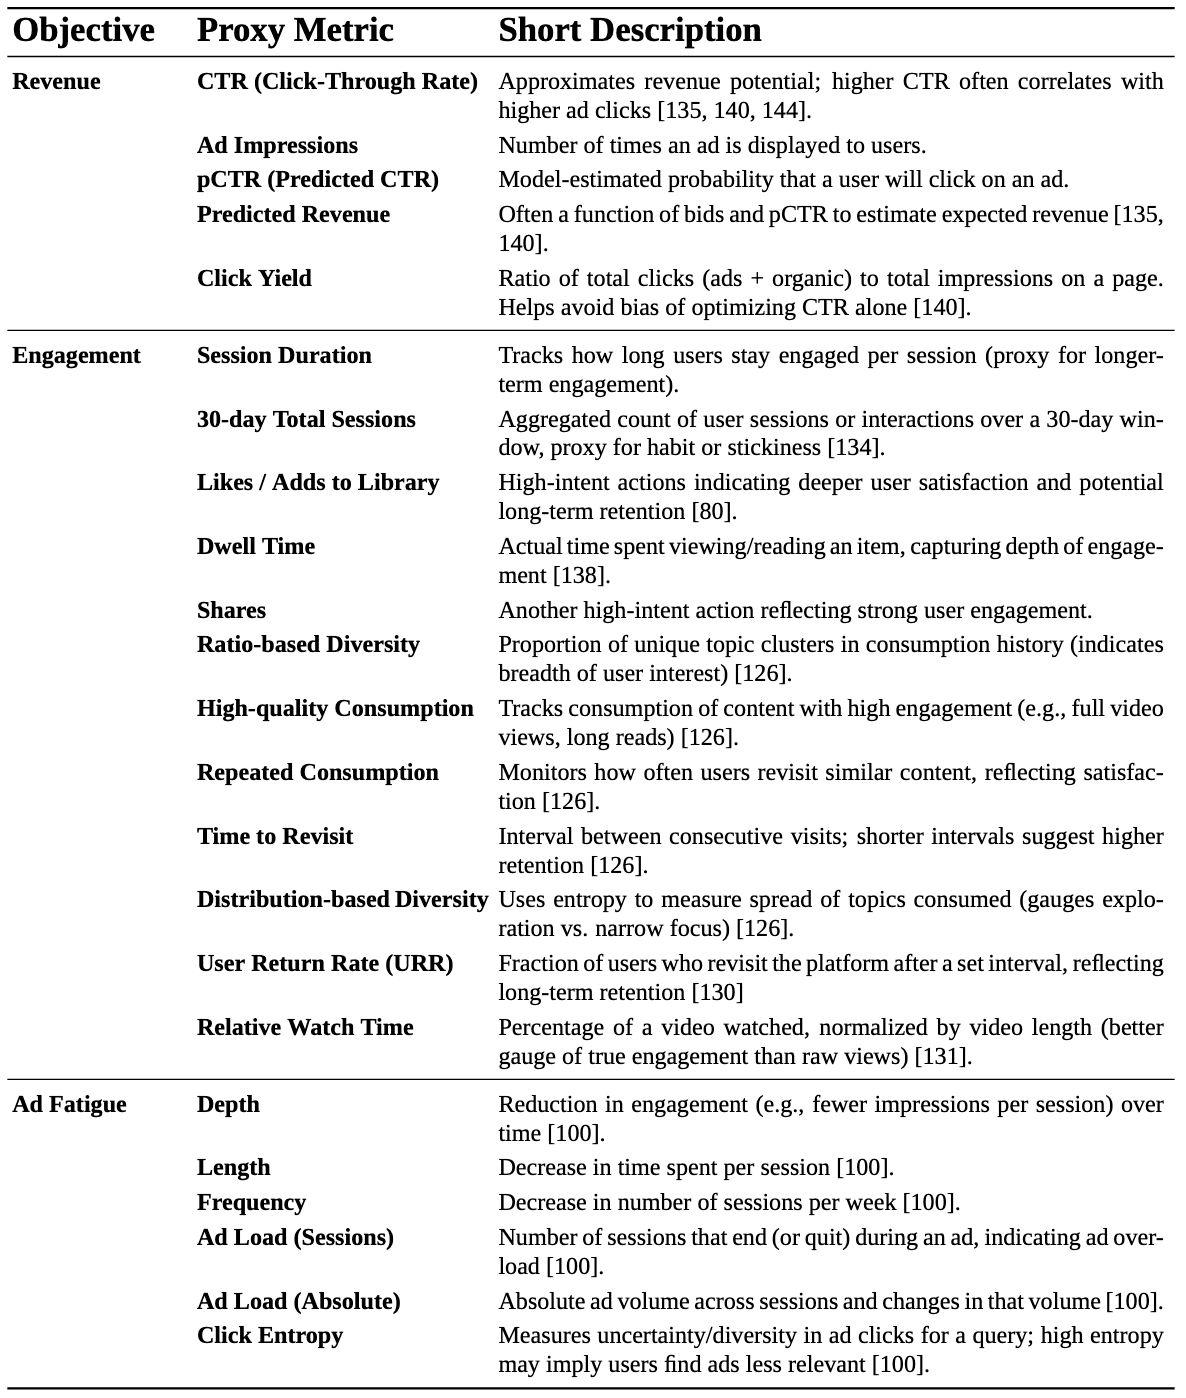
\includegraphics[width=\linewidth]{proxy-metrics-table.png}
% \caption{Proxy metrics for Revenue, Engagement, and Ad Fatigue.}
% \label{fig:proxy-metrics}
% \end{figure}

\begin{figure}[ht]
  \centering
  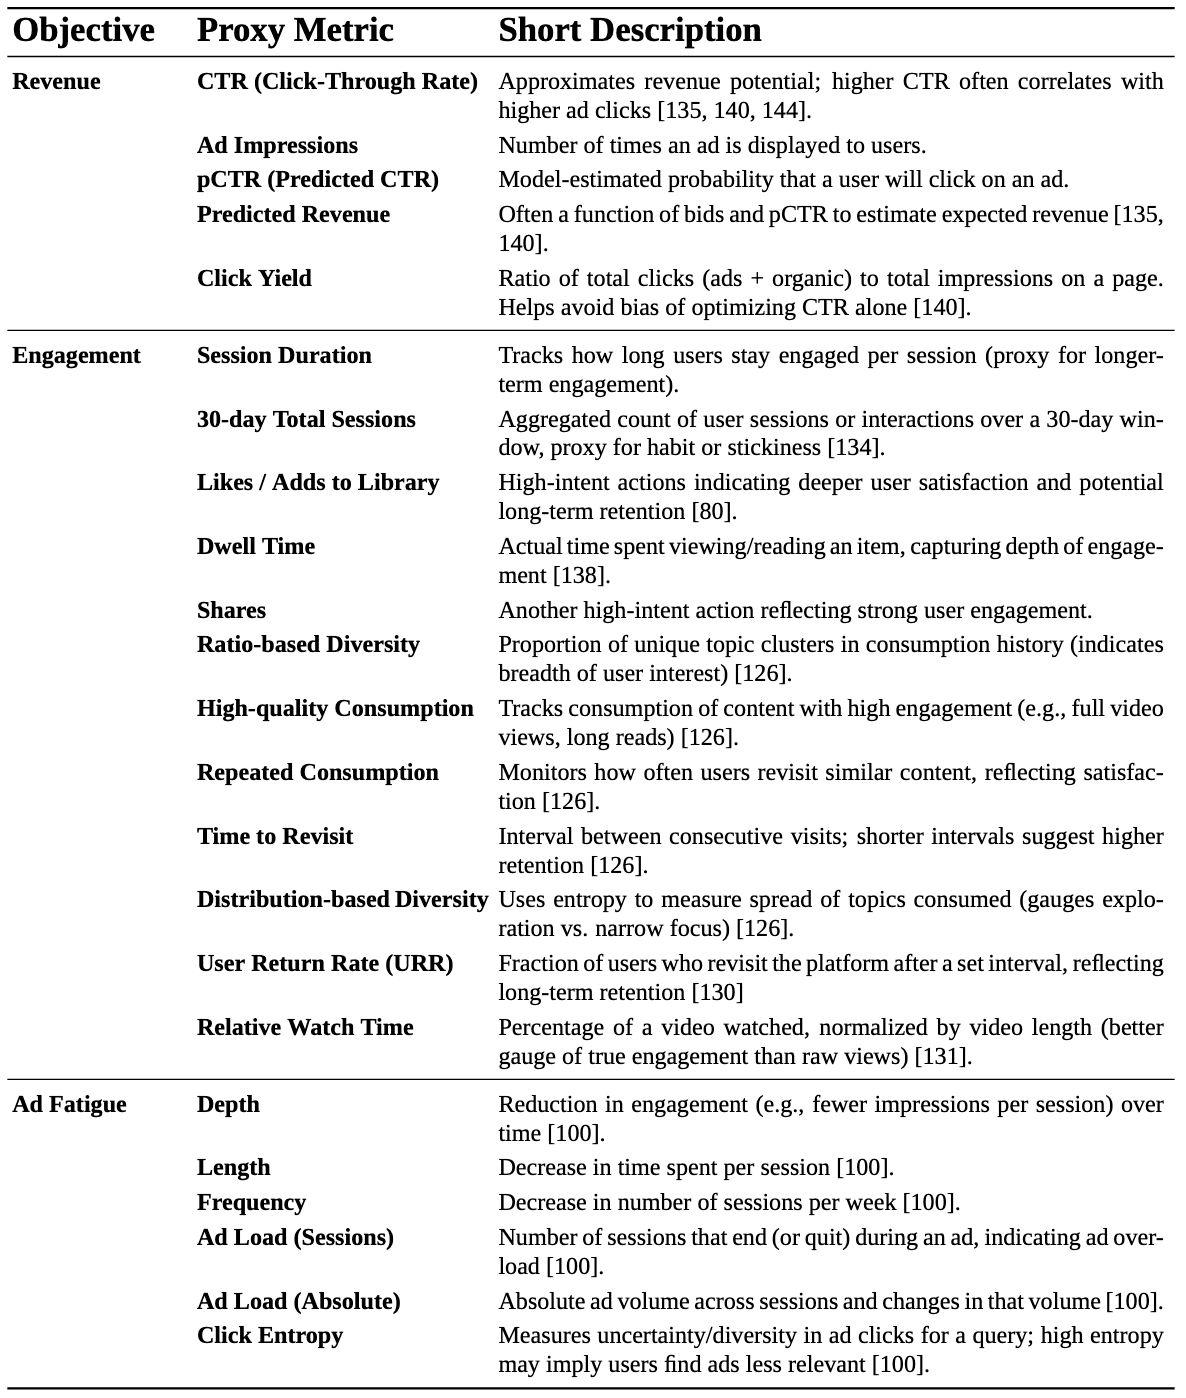
\includegraphics[width=\textwidth, height=0.85\textheight, keepaspectratio]{proxy-metrics-table.png}
  \caption{Proxy metrics for Revenue, Engagement, and Ad Fatigue.}
  \label{fig:proxy-metrics}
\end{figure}


% \begin{table}[H]
% \setstretch{1} % Ensure normal spacing within table. Separation between lines of the same cell. 
% \centering
% \small
% \renewcommand{\arraystretch}{1.2}  % Tweak if needed
% \setlength{\tabcolsep}{2pt} % separation between columns 
% \begin{tabularx}{\linewidth}{p{0.15\linewidth} p{0.25\linewidth} p{0.57\linewidth}}
% % the decimal points allow to control the size of the table, not of the text.
% \toprule
% {\bfseries \Large Objective} & {\bfseries \Large Proxy Metric} & {\bfseries \Large Short Description} \\
%   % \textbf{Objective} & \textbf{Proxy Metric} & \textbf{Short Description} \\
% \midrule
%     \multirow{\textbf{Revenue}} 
%        & \textbf{CTR (Click-Through Rate)} 
%            &  Approximates revenue potential; higher CTR often correlates with higher ad clicks \cite{zhang2018whole, yan2020ads, zhao2020jointly}. \\
%        & \textbf{Ad Impressions} 
%            & Number of times an ad is displayed to users. \\
%        & \textbf{pCTR (Predicted CTR)} 
%            & Model-estimated probability that a user will click on an ad. \\
%        & \textbf{Predicted Revenue} 
%            & Often a function of bids and pCTR to estimate expected revenue  \cite{yan2020ads, zhang2018whole}. \\
%        & \textbf{Click Yield} 
%            & Ratio of total clicks (ads + organic) to total impressions on a page. Helps avoid bias of optimizing CTR alone \cite{zhang2018whole}. \\
%     \midrule
%     \multirow{\textbf{Engagement}} 
%        & \textbf{Session Duration} 
%            & Tracks how long users stay engaged per session (proxy for longer-term engagement). \\
%         & \textbf{30-day Total Sessions} 
%        & Aggregated count of user sessions or interactions over a 30-day window, proxy for habit or stickiness 
%        \cite{xu2023optimizing}. \\
%        & \textbf{Likes / Adds to Library} 
%        & High-intent actions indicating deeper user satisfaction and potential long-term retention \cite{mcdonald2023spotify}. \\
%           & \textbf{Dwell Time} 
%        & Actual time spent viewing/reading an item, capturing depth of engagement  \cite{yi2014beyond}. \\
%        & \textbf{Shares} 
%            & Another high-intent action reflecting strong user engagement. \\
%     & \textbf{Ratio-based Diversity}  
%            & Proportion of unique topic clusters in consumption history (indicates breadth of user interest) \cite{wang2022surrogate}. \\
%        & \textbf{High-quality Consumption} 
%            & Tracks consumption of content with high engagement (e.g., full video views, long reads) \cite{wang2022surrogate}. \\
%      & \textbf{Repeated Consumption}  
%            & Monitors how often users revisit similar content, reflecting satisfaction \cite{wang2022surrogate}. \\
%               & \textbf{Time to Revisit} 
%            & Interval between consecutive visits; shorter intervals suggest higher retention \cite{wang2022surrogate}. \\
%      & \textbf{Distribution-based Diversity}  
%            & Uses entropy to measure spread of topics consumed (gauges exploration vs. narrow focus) \cite{wang2022surrogate}. \\
%     & \textbf{User Return Rate (URR)} 
%        & Fraction of users who revisit the platform after a set interval, reflecting long-term retention  \cite{wu2017returning} \\
%      & \textbf{Relative Watch Time} 
%        & Percentage of a video watched, normalized by video length (better gauge of true engagement than raw views) 
%       \cite{wu2018beyond}. \\
%     \midrule
%     \multirow{\textbf{Ad Fatigue}} 
%        & \textbf{Depth} 
%            & Reduction in engagement (e.g., fewer impressions per session) over time \cite{sagtani2023quantifying}. \\
%        & \textbf{Length} 
%            & Decrease in time spent per session \cite{sagtani2023quantifying}. \\
%        & \textbf{Frequency} 
%            & Decrease in number of sessions per week \cite{sagtani2023quantifying}. \\
%        & \textbf{Ad Load (Sessions)} 
%            & Number of sessions that end (or quit) during an ad, indicating ad overload \cite{sagtani2023quantifying}. \\
%        & \textbf{Ad Load (Absolute)} 
%            & Absolute ad volume across sessions and changes in that volume \cite{sagtani2023quantifying}. \\
%        & \textbf{Click Entropy} 
%            & Measures uncertainty/diversity in ad clicks for a query; high entropy may imply users find ads less relevant \cite{sagtani2023quantifying}. \\
% \bottomrule
% \end{tabularx}
% \caption{Proxy metrics for Revenue, Engagement, and Ad Fatigue.}
% \label{tab:proxy-metrics}
% \end{table}




\textbf{Utility functions are mathematical constructs used to estimate the net value of conflicting objectives \cite{Stigler1950}.} A utility function is a \textbf{composite reward function} that allows the agent to integrate various rewards or metrics from multiple objectives using a unified currency, facilitating more nuanced decision-making across competing priorities \cite{Stigler1950}. The ability to compare two utilities, like those of revenue and engagement normalized to a common scale, is critical for any principled blending of organic items and ads \cite{yan2020ads}.  Most utility functions are linear though this linearity is not a requirement for how the individual utility of each component is calculated \cite{wen2019learning, zhao2020jointly}. 

A \textbf{canonical utility function} at the policy layer to \textit{blend} ads and organic content can be represented as follows \cite{sagtani2024ad, yan2020ads, carrion2021blending}:
    \begin{equation}
        U(x) = \alpha \times \text{Revenue} + \beta \times \text{Engagement} - \gamma \times \text{Ad Fatigue}
    \end{equation}
    where $\alpha$, $\beta$, and $\gamma$ are weights that determine the relative importance of each factor. To compute the utilities of "Revenue", "Engagement", and "Ad Fatigue", typically many signals feed into each component. These signals include, but are not limited to, the ones shown in Table \ref{fig:proxy-metrics}. In a bandit or RL context, $U(x)$ serves as the reward signal guiding policy updates. The process of tuning the weights of $\alpha$, $\beta$, and $\gamma$ is often done through experimentation, as the right balance between engagement and revenue can shift depending on the context. For instance, ByteDance uses a multi-objective reward framework in their recommendation systems, where different reward functions are designed for organic content and ads, combining them to guide the overall recommendation strategy \cite{zhao2020jointly}.
    
In some cases, a very simple unified function can suffice over a complex utility function. Researchers at Alibaba introduced the concept of Click Yield, which is defined as the ratio of the total number of clicks on all items (ads + organic results) to the total number of impressions on a page \cite{zhang2018whole}. Click Yield provides a holistic evaluation of page performance, accounting for the interactive effects between ads and organic content, and helping to mitigate the bias that arises from examining CTR in isolation. Their optimization task maximizes total revenue while ensuring that the Click Yield does not fall below a certain threshold (T)  \cite{zhang2018whole}. A comparison of utility function formulations is shown in Table \ref{fig:utility-comparison}.

\begin{figure}[ht]
\centering
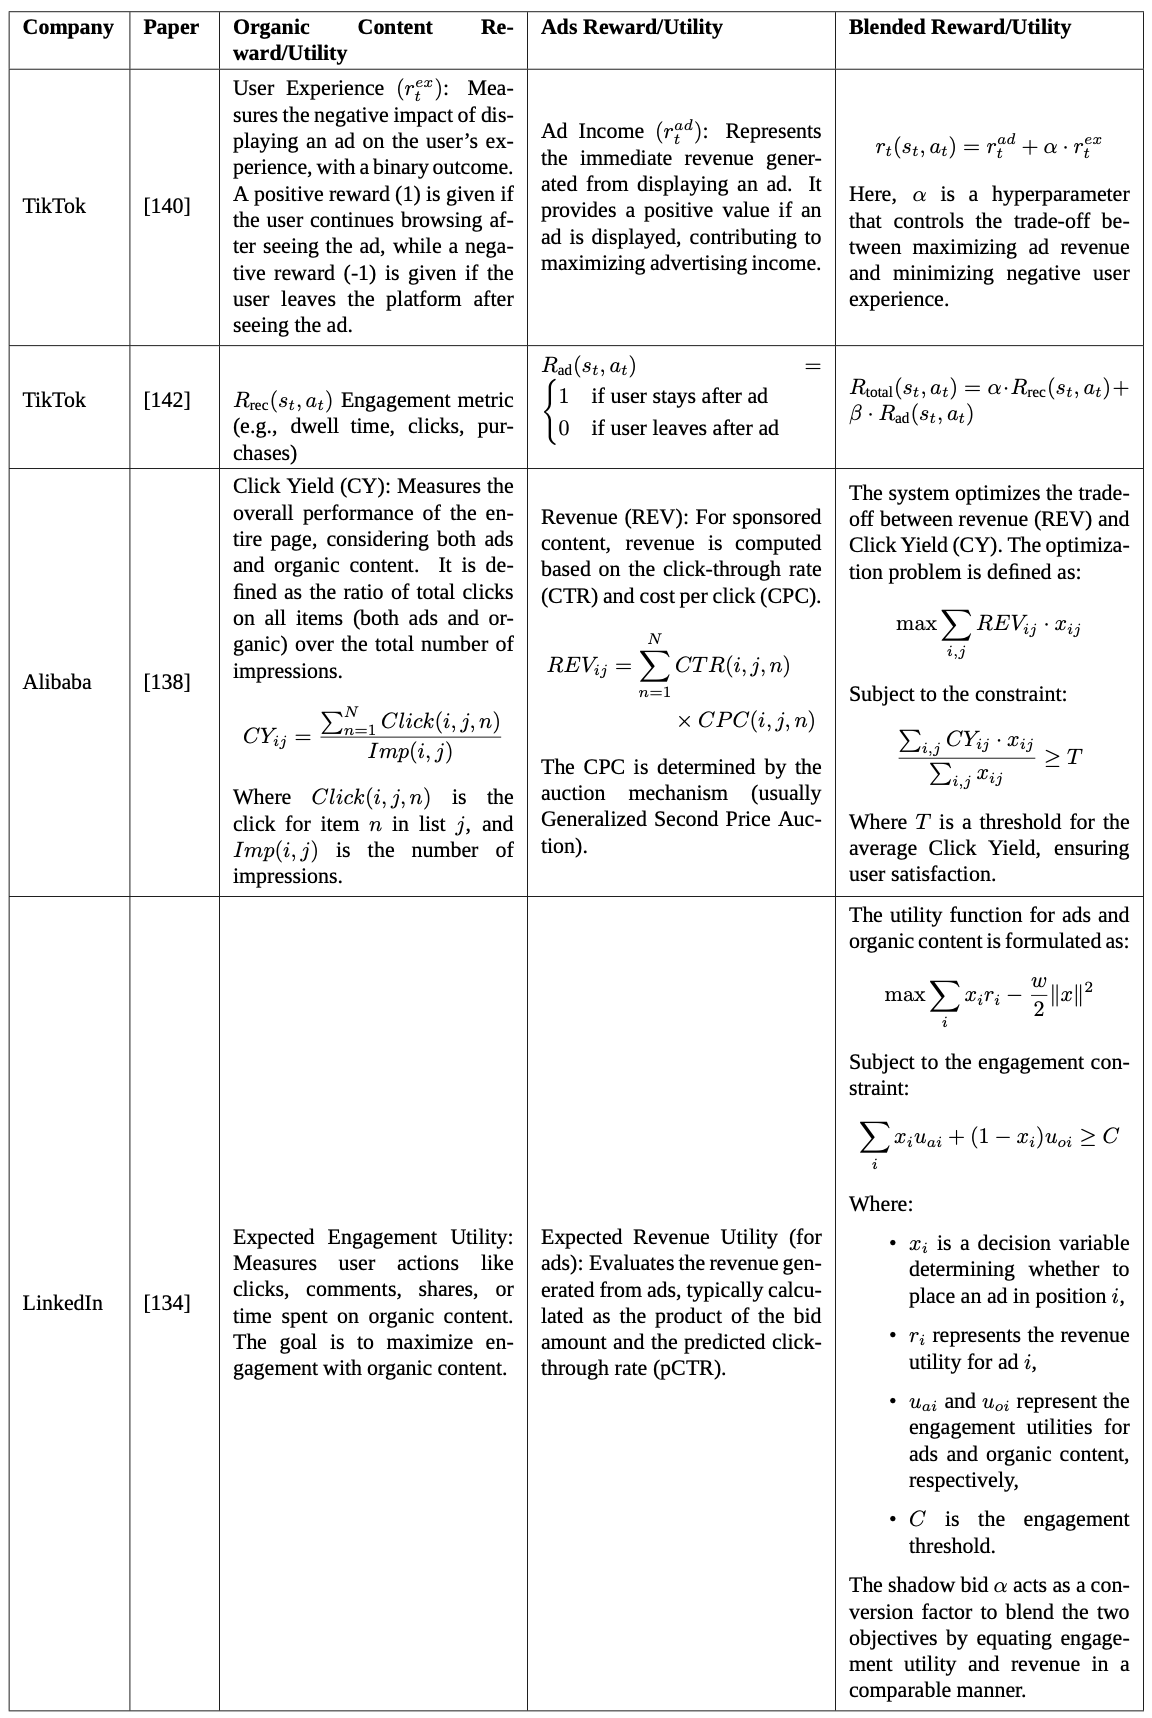
\includegraphics[width=\textwidth, height=0.85\textheight, keepaspectratio]{utility-comparison-table.png}
\caption{Comparison of Utility/Reward Formulation Approaches across Different Companies}
\label{fig:utility-comparison}
\end{figure}



% Adjusted table with better column width control and proper spacing
% \begin{table}[ht]
%     \centering
%     % \renewcommand{\arraystretch}{1.3}  % Adjust row height spacing
%     \begin{adjustbox}{max width=\textwidth}
%     \small % Decrease font size for the table
%     % \setlength{\tabcolsep}{6t} % Increase spacing between text and vertical lines
%     \renewcommand{\arraystretch}{1.15}
% \begin{tabular}{|p{1.5 cm}|p{1 cm}|p{4.5 cm}|p{4.5 cm}|p{4.5 cm}|}
%     \hline
%     \textbf{Company} & \textbf{Paper} & \textbf{Organic Content Reward/Utility} & \textbf{Ads Reward/Utility} & \textbf{Blended Reward/Utility} \\ 
%     \hline
%     TikTok & \cite{zhao2021dear} & 
%     \begin{minipage}{4.5cm}
%     \vspace{4pt}
%         User Experience \((r_t^{ex})\): Measures the negative impact of displaying an ad on the user's experience, with a binary outcome. A positive reward (1) is given if the user continues browsing after seeing the ad, while a negative reward (-1) is given if the user leaves the platform after seeing the ad.
%         \vspace{4pt}
%     \end{minipage}
%     & 
%     \begin{minipage}{4.5cm}
%     \vspace{4pt}
%         Ad Income \((r_t^{ad})\): Represents the immediate revenue generated from displaying an ad. It provides a positive value if an ad is displayed, contributing to maximizing advertising income.
%         \vspace{4pt}
%     \end{minipage}
%     & 
%     \begin{minipage}{4.5cm}
%     \vspace{4pt}
%         \[
%         r_t(s_t, a_t) = r_t^{ad} + \alpha \cdot r_t^{ex}
%         \]
%         Here, \(\alpha\) is a hyperparameter that controls the trade-off between maximizing ad revenue and minimizing negative user experience.
%         \vspace{4pt}
%     \end{minipage} \\
%     \hline
%     TikTok & \cite{zhao2020jointly} & 
%     $R_{\text{rec}}(s_t, a_t)$ Engagement metric (e.g., dwell time, clicks, purchases)  
%     & 
%     \begin{minipage}{4.5cm}
%     \vspace{4pt} 
%     \( R_{\text{ad}}(s_t, a_t) = 
%     \begin{cases} 
%         1 & \text{if user stays after ad} \\
%         0 & \text{if user leaves after ad} 
%     \end{cases} \) 
%         \vspace{4pt}
%     \end{minipage}
%     & 
%     \begin{minipage}{4.5cm}
%     \vspace{4pt}
%     \( R_{\text{total}}(s_t, a_t) = \alpha \cdot R_{\text{rec}}(s_t, a_t) + \beta \cdot R_{\text{ad}}(s_t, a_t) \)
%         \vspace{4pt}
%     \end{minipage} \\
%     \hline
%     Alibaba & \cite{zhang2018whole} & 
%     \begin{minipage}{4.5cm}
%     \vspace{4pt}
%         Click Yield (CY): Measures the overall performance of the entire page, considering both ads and organic content. It is defined as the ratio of total clicks on all items (both ads and organic) over the total number of impressions.
%         \[
%         CY_{ij} = \frac{\sum_{n=1}^{N} Click(i, j, n)}{Imp(i, j)}
%         \]
%         Where \(Click(i, j, n)\) is the click for item \(n\) in list \(j\), and \(Imp(i, j)\) is the number of impressions.
%         \vspace{4pt}
%     \end{minipage}
%     & 
%     \begin{minipage}{4.5cm}
%     \vspace{4pt}
%         Revenue (REV): For sponsored content, revenue is computed based on the click-through rate (CTR) and cost per click (CPC).
%         \[
% \begin{aligned}
% REV_{ij} = \sum_{n=1}^{N} & \, CTR(i, j, n) \\
% & \times CPC(i, j, n)
% \end{aligned}
% \]
%         The CPC is determined by the auction mechanism (usually Generalized Second Price Auction).
%         \vspace{4pt}
%     \end{minipage}
%     & 
%     \begin{minipage}{4.5cm}
%     \vspace{4pt}
%         The system optimizes the trade-off between revenue (REV) and Click Yield (CY). The optimization problem is defined as:
%         \[
%         \max \sum_{i,j} REV_{ij} \cdot x_{ij}
%         \]
%         Subject to the constraint:
%         \[
%         \frac{\sum_{i,j} CY_{ij} \cdot x_{ij}}{\sum_{i,j} x_{ij}} \geq T
%         \]
%         Where \(T\) is a threshold for the average Click Yield, ensuring user satisfaction.
%         \vspace{4pt}
%     \end{minipage} \\
%     \hline
%     LinkedIn & \cite{yan2020ads} & 
%     \begin{minipage}{4.5cm}
%     \vspace{4pt}
%         Expected Engagement Utility: Measures user actions like clicks, comments, shares, or time spent on organic content. The goal is to maximize engagement with organic content.
%         \vspace{4pt}
%     \end{minipage}
%     & 
%     \begin{minipage}{4.5cm}
%     \vspace{4pt}
%         Expected Revenue Utility (for ads): Evaluates the revenue generated from ads, typically calculated as the product of the bid amount and the predicted click-through rate (pCTR).
%         \vspace{4pt}
%     \end{minipage}
%     & 
%     \begin{minipage}{4.5cm}
%     \vspace{4pt}
%         The utility function for ads and organic content is formulated as:
%         \[
%         \max \sum_i x_i r_i - \frac{w}{2} \| x \|^2
%         \]
%         Subject to the engagement constraint:
%         \[
%         \sum_i x_i u_{ai} + (1 - x_i) u_{oi} \geq C
%         \]
%         Where:
%         \begin{itemize}
%             \item \(x_i\) is a decision variable determining whether to place an ad in position \(i\),
%             \item \(r_i\) represents the revenue utility for ad \(i\),
%             \item \(u_{ai}\) and \(u_{oi}\) represent the engagement utilities for ads and organic content, respectively,
%             \item \(C\) is the engagement threshold.
%         \end{itemize}
%         The shadow bid \(\alpha\) acts as a conversion factor to blend the two objectives by equating engagement utility and revenue in a comparable manner.
%         \vspace{4pt}
%     \end{minipage} \\
%     \hline
% \end{tabular}
% \end{adjustbox}
% \caption{Comparison of Utility/Reward Formulation Approaches across Different Companies}
% \label{tab:utility-comparison}
% \end{table}


\subsection{Action Space Representation}
\label{action_space_representation}

In RL, environments are modeled as a Markov Decision Process (MDP). An MDP is defined by $(\mathcal{S}, \mathcal{A}, P, R)$, where $\mathcal{S}$ is the state space, $\mathcal{A}$ is the action space, $P(\cdot\mid s,a)$ is the transition probability distribution, and $R(s,a)$ is the reward function. At each timestep $t$, the agent observes a state $s_t \in \mathcal{S}$ and selects an action $a_t \in \mathcal{A}$. Both action and state sets may be finite, infinite, discrete, or continuous.

% What is an action 
In RL, an \textbf{action} $a \in \mathcal{A}$ refers to \textbf{a decision or intervention taken by the agent based on its current state to influence the environment} \cite{Sutton1998}. The action space $\mathcal{A}$  represents the complete set of all possible actions that the agent can choose from at any given decision point \cite{Sutton1998}. For example, in the  FrozenLake environment,\textbf{ the possible actions for the agent are \textit{up, down, left} and \textit{right}} \cite{frozenlake}. \textbf{Because this set of possible actions is countable, the action space for the FrozenLake is said to be \textit{discrete} \cite{frozenlake}.} By contrast, in an \emph{advertisement recommendation} setting, the action space $\mathcal{A}$ might consist of all possible combinations of ads, their rankings, placements, and formats \cite{ie2019slateq}. The objective of this set of actions in ad recommendation is to deliver the right set of ads at the right time in order to maximize platform revenue, while maintaining or improving user engagement and satisfaction \cite{zhao2020jointly}. Although this action space is discrete and countable, the number of possible combinations grows exponentially with the number of candidate ads and available slots. As a result, it becomes computationally infeasible to enumerate or evaluate each action individually, and must instead be treated using methods designed for high-dimensional discrete spaces \cite{ie2019recsim}.

\textbf{An ideal action space should be \textit{expressive} enough to capture all relevant degrees of freedom the agent needs to optimize its behavior, but it should avoid unnecessary complexity \cite{zhu2024discretizing, liu2025reducing}.} The action space described above in the FrozenLake example satisfies these criteria, as the four cardinal movements (\textit{up, down, left,} and \textit{right}) are enough to navigate to any state in the grid while remaining \textbf{orthogonal}, thus providing both sufficient \textbf{coverage and simplicity} \cite{frozenlake}.  In contrast, the ad recommendation action space is inherently high-dimensional and entangled \cite{ie2019recsim}. The agent must decide \emph{what} to show (a discrete choice over candidate ads), \emph{where} to place it  (which may be modeled as a discrete slot or a continuous position), and in \emph{what order} (often determined by continuous relevance scores), often under tight latency constraints and user personalization requirements \cite{zhao2020jointly}. The action space in ad recommendation systems must be expressive enough to encompass all relevant choices for optimal ad delivery while ensuring no combinatorial explosion in complexity \cite{ie2019slateq}. Moreover, ensuring that each dimension remains sufficiently \emph{orthogonal} can be nontrivial, given potential interactions between ad content, positioning, and user context \cite{ie2019reinforcement}. If the action space is too coarse, the system risks underfitting, serving generic policies that fail to personalize effectively or miss monetization opportunities \cite{ie2019slateq}. On the other hand, if it is too fine, the system may overfit to noise, struggle to generalize, or incur prohibitive computational costs \cite{ie2019slateq}. Practical systems often resort to action abstraction or parameterization (e.g., slate-based policies, ad load knobs, or policy buckets) to reduce complexity at the cost of optimality \cite{ie2019reinforcement, hohnhold2015focusing, sagtani2024ad}.

\textbf{The independence of these action dimensions facilitates more modular policy learning \cite{tavakoli2018action, sharma2017learning}}. By allowing a degree of independence for each action dimension, the agent achieves modular policy learning that scales linearly (instead of exponentially) with the number of action degrees-of-freedom \cite{tavakoli2018action}. In addition, actions should ideally correspond to \textbf{semantically meaningful choices} to facilitate policy interpretability and validation \cite{glanois2024survey, puiutta2020explainable}. In the case of the FrozenLake problem, the action space is intuitive and human-interpretable, making it straightforward to validate learned policies \cite{brockman2016openai, Sutton1998}. For instance, an RL practitioner can manually inspect and reason about the learned policy (e.g. "the agent plans to move \textit{down} then \textit{right} to reach the goal") to verify that each action choice aligns with domain logic \cite{brockman2016openai}. While the action space in ad recommendation systems is far more complex, structuring it around semantically meaningful levers (e.g., “increase ad load for high-intent users” or “downrank low-quality creatives”) enables engineers and product teams to reason about the system’s behavior \cite{glanois2024survey, dulac2021challenges}. If a learned policy increases ad load for a particular user segment, analysts can trace this decision back to upstream signals, such as historical engagement patterns or commercial intent scores \cite{gauci2018horizon, dulac2021challenges}. Policies composed of interpretable levers enable more transparent debugging, offline validation, and policy review, which is crucial for ensuring that the deployed strategy aligns with business intuition, avoids learning spurious correlations, and mitigates the risk of unintended outcomes \cite{dulac2021challenges, verma2018programmatically, puiutta2020explainable, glanois2024survey}.

\textbf{Moreover, an action space should be consistent across episodes \cite{puterman2014markov}.} That is, taking the same action in the same state should yield statistically predictable outcomes \cite{puterman2014markov}. \textbf{The state space in the FrozenLake is stochastic \cite{frozenlake}}, meaning that taking the same action does not always result in the same next state. For example, selecting the action "move right" might result in the agent moving right, up, or down, as governed by the transition probabilities defined by $P(s' \mid s, a)$ \cite{frozenlake}. Despite the stochasticity in the environment,\textbf{ the outcomes observed should converge to the expected values described by the transition probability distribution over a sufficiently large number of episodes \cite{puterman2014markov}}. A similar principle applies in ad recommendation. Although user behavior and auction dynamics introduce stochasticity, \textbf{taking the same ad-serving action, such as presenting a specific slate of ads to a user with a given context, should yield statistically predictable engagement or monetization outcomes}. That is, over many episodes, \textbf{the distribution of observed rewards (e.g., clicks, conversions, revenue) should converge to the expected value associated with the given state-action pair \cite{mcmahan2013ad, zhao2018deep}}. This consistency is foundational for policy learning, as it ensures that repeated exposure to similar decision contexts enables accurate estimation of long-term value, despite noisy observations \cite{Sutton1998}. 

The action space can be thought of as levers that can be used to tune ad policy. Typical \textbf{levers in treatments in ad policies} include the following elements \cite{koutsopoulos2016native}: 

\begin{itemize}
    \item \textbf{Ad Load.} Also referred to as the spacing ads or frequency of ads is also a key component in inducing ad load fatigue. Placing ads too closely together may lead to user fatigue and reduced click probabilities \cite{abrams2007personalized, zhao2020jointly}. 
    \item \textbf{Ad Quality.} This refers to intrinsic features of the ad, such as the design format, product type, accompanying text, and the quality of the landing page, all of which directly influence user engagement. \cite{yan2009much, nielsen2017advertising}.
    \item \textbf{Ad Placement.}
Ads placed earlier in the feed are more likely to be clicked, though their relevance to preceding content also plays a significant role \cite{zhao2020jointly, saha2021advertiming, yuan2020unbiased}. 
    \item \textbf{Ad Relevance.} Ads that align more closely with user preferences and user intent are more likely to drive engagement. For example, an ad on a hotel might have a higher probability if shown adjacent to results of search queries related to vacations \cite{chakrabarti2008contextual, Zhou2018}. \\
\end{itemize}

\subsection{State Space Representation} \label{state_space_representation}
% Definition and Desirable Properties
% 1.1 What is a state space in RL?
% 1.2 Desirable properties of a state space
% Markovianity
% Expressiveness vs. generalization
% Stability under distribution shift
% Sample efficiency and learnability
% Interpretability and support for counterfactual reasoning

In RL, a \textit{state} $s \in \mathcal{S}$  represents all the relevant information from past agent-environment interactions necessary for the agent to make optimal decisions to maximize the expected cumulative reward \cite{Sutton1998}. Ideally, the state space is Markovian, meaning the future is conditionally independent of the past given the current state \cite{russell2016artificial, Sutton1998}. If the agent’s policy or value estimates rely on omitted or unobserved information from the past, the state representation violates the Markov property and the performance of the learned policy may degrade as a result \cite{russell2016artificial, Sutton1998}. In the FrozenLake example, the state space consists of the agent’s current grid position as the future outcomes of any action depend only on this position, and not on how the agent arrived there \cite{frozenlake}. In this example, because future transitions depend only on the current state and action, and not on prior history, the FrozenLake Environment satisfies the \textit{Markov Property} \cite{Sutton1998, frozenlake}.  


In contrast, the environments where \textbf{ad recommendation systems} operate are often \textbf{partially observable, high-dimensional, and non-stationary} \cite{dulac2021challenges, russell2016artificial}. To construct a state representation that reasonably approximates the Markov property in the face of partial observability and complex user dynamics, ad recommendation systems often combine tabular features with learned embeddings \cite{afsar2022reinforcement, kaelbling1998planning}. The tabular signals tend to include static attributes (e.g. demographics), contextual metadata (e.g. device type, time of the day), and behavioral history (e.g. recent clicks, impressions, or dwell time) \cite{cheng2016wide, covington2016deep}. An embedding is a learned, dense vector that encodes complex or high-cardinality inputs, such as user profiles, ads, or behavioral sequences, into a lower-dimensional space \cite{cheng2016wide}. Compared to static tabular features like frequency counts or recency buckets, embeddings capture richer structure, including sequence effects and latent similarity. This makes them more expressive and task-relevant, enabling ad recommendation systems to personalize content and ads more effectively \cite{covington2016deep, cheng2016wide}.

% User embeddings, item embeddings, user-item interaction embeddings, and sequence embeddings are among the most common embedding types used in recommendation systems. Each embedding type captures distinct aspects of information to guide the agent’s decisions. 

% Contextual features, including a user's location or device type, often serve as informative priors, particularly helpful in addressing the cold-start problem, i.e., when new users enter an ecosystem with limited historical data \cite{covington2016deep}. Additionally, some platforms prompt new users to select interests or topics during onboarding, providing supplementary signals that help initialize user embeddings. When no data for users is available (incognito window, SEO-driven traffic, new device without login, etc), systems typically default to population-level trends or popular content. While user embeddings may also be static and updated on batch mode, user embeddings can also be updated dynamically, such that as users engage further, the continuous updates on the embeddings allow for more personalized policies by the agent to reflect new information in the system and evolving preferences.

Embeddings may consist of two components: an offline (stationary) component and an online (non-stationary) component \cite{zhao2023embedding}. \textbf{Offline embeddings} represent \textbf{stationary or slow-changing attributes}, such as a user's demographics (e.g., gender, country) or long-term preferences, and fixed item properties (e.g., brand or product category) \cite{koren2009matrix, quadrana2018sequence}. These embeddings are usually computed in batch mode due to their \textbf{higher computational complexity, larger size, and relatively static nature} \cite{naumov2019deep, liu2022monolith}. \textbf{Online embeddings}, conversely, address non-stationary and rapidly evolving aspects such as recent user behaviors, trending content, or immediate interests \cite{Zhou2018, zhou2019deep}. These embeddings are \textbf{generally smaller,} \textbf{computed in near-real-time to meet latency requirements} \cite{liu2022monolith}. This hybrid approach combines stable and dynamic embeddings, balancing relevance with computational efficiency \cite{cheng2016wide, covington2016deep}. Furthermore, this allows the recommendation system to remain stable under distribution shifts, which is of paramount importance, especially in environments with rapidly evolving user preferences, content inventories, and behavioral patterns \cite{gama2014survey, Sutton1998}.

To effectively integrate diverse embeddings (user, item, interaction) and their offline and online components, embeddings of varying dimensions are typically concatenated and then projected via learned linear layers into a shared dimension \cite{pancha2022pinnerformer, grbovic2018real, covington2016deep}. Generally, zero-padding or truncation is avoided, as these methods can introduce noise or cause information loss \cite{xia2023transact}.

\textbf{User embeddings} are learned vector representations designed to capture user preferences and behaviors, enabling ad recommendation systems to personalize content effectively at scale \cite{covington2016deep, he2017neural}. These embeddings compress complex, high-dimensional user data, such as past interactions and demographic information, into compact vectors utilized by recommendation models \cite{covington2016deep, koren2009matrix, naumov2019deep}. User embeddings can be learned using a combination of supervised, unsupervised, and self-supervised approaches \cite{zhao2021dear}.  In the case of supervised learning, embeddings are optimized to predict explicit labels such as clicks, conversions, or purchases \cite{covington2016deep, Zhou2018}. To exploit information in more implicit signals, self-supervised methods can be used with objectives such as next item interaction or item co-occurrence \cite{yuan2020unbiased, mikolov2013distributed}. Many practical implementations tend to combine both supervised and self-supervised methods \cite{zhao2021dear, xia2023transact}. For example, embeddings may initially be learned through self-supervised tasks (e.g., predicting next clicks) and then fine-tuned on supervised tasks (CTR, conversions). A well-documented example is that of YouTube, where despite the availability of explicit feedback mechanisms (thumbs up/down, in-product surveys, etc.), they turn to implicit signals, where a user completing a video is a positive example, given that the relative prevalence of implicit signals is much higher than explicit signals, allowing the models to learn more effectively \cite{covington2016deep}.

\textbf{Item embeddings} are designed to capture intrinsic item characteristics \cite{koren2009matrix}. These embeddings compress complex, high-dimensional item data, such as product descriptions, categories, brands, and historical interaction patterns \cite{koren2009matrix, cheng2016wide}. Similar to user embeddings, item embeddings can be learned through supervised, unsupervised, and self-supervised approaches \cite{barkan2016item2vec, zhao2023embedding}. In supervised learning scenarios, embeddings are optimized to predict explicit labels, such as clicks, conversions, or purchases associated with the items \cite{covington2016deep, naumov2019deep}. To leverage more implicit information, self-supervised methods may focus on objectives like predicting co-occurrence patterns or sequential interactions (e.g., item-to-item relationships) \cite{barkan2016item2vec, sun2019bert4rec}. 

While user and item embeddings provide essential representations of individual entities, it is through interaction embeddings, which capture the joint dynamics between users and items, that the system truly learns user preferences and can surface content that is contextually relevant and personalized \cite{koren2009matrix}. Being able to \textbf{ effectively represent user-item interactions} is at the core of personalization for recommendation systems \cite{linden2003amazon}. Collaborative Filtering (CF) was one of the earliest popular methods to represent user-item interactions \cite{linden2003amazon, Bobadilla2013}. CF predicted user preferences by analyzing explicit interactions (e.g., ratings) or implicit behavioral signals (e.g., clicks, views), using metrics like cosine similarity or Pearson correlation \cite{Bobadilla2013}. However, CF struggled with sparse datasets, as many user-item pairs lacked interactions, limiting recommendation accuracy \cite{Bobadilla2013}. Additionally, CF's direct interaction-based approach limited its ability to capture deeper latent or implicit relationships between users and items \cite{koren2008factorization}.

Matrix Factorization (MF), popularized during the Netflix Prize competition (2006–2009), addressed some of CF’s key limitations \cite{bennett2007netflix}. The classic approach is to factorize the (sparse) interaction matrix into the product of a user-factor matrix and an item-factor matrix \cite{koren2009matrix}. MF learns these latent (hidden) user and item factors by optimizing embeddings to reconstruct observed interactions, enabling it to capture deeper relational structures that CF missed \cite{koren2009matrix}. MF also significantly improved storage efficiency \cite{koren2009matrix}. For instance, a CF matrix with 1 million users and 1 million items would contain 1 trillion (mostly sparse) entries. In contrast, MF represents these interactions using two dense embedding matrices totaling approximately 128 million entries (assuming an embedding dimension of k=64) \cite{koren2009matrix}.

As companies began logging large-scale user interaction data in the late 2000s and early 2010s, Amazon, Spotify, and Netflix turned to Matrix Factorization (MF) as a simple yet effective way to harness that data for scalable personalization \cite{gomez2015netflix, linden2003amazon}. However, while MF improved predictions for existing users/items with limited interactions, it did not solve all limitations of CF \cite{koren2009matrix}. Particularly, MF still struggled with the cold-start problem, as completely new users or items without interaction history cannot be effectively represented in the embedding space \cite{koren2009matrix}. Additionally, MF assumes linear interactions between latent factors, limiting its ability to capture more complex, nonlinear user behaviors \cite{he2017neural}. Neural embeddings emerged in the 2010s to address some of these limitations \cite{he2017neural}. Unlike CF and MF, neural embeddings naturally capture complex, nonlinear interactions between users and items \cite{he2017neural}. They also effectively incorporate content-based and contextual metadata, significantly improving the handling of cold-start issues \cite{van2013deep, cheng2016wide, naumov2019deep}. Two-tower models,  notably introduced by Google for YouTube’s recommendation systems, leverage deep neural networks for scalable candidate retrieval and generation \cite{covington2016deep}.  A two-tower model consists of two distinct neural network components: one tower encodes user-specific features, and the other one encodes item-specific features, projecting them into a shared latent embedding space \cite{covington2016deep}. This shared embedding space enables efficient similarity computation, facilitating large-scale real-time recommendations \cite{covington2016deep}. Today, companies like YouTube use two-tower models for tasks such as next-video prediction, and Meta uses them for personalized ad ranking \cite{covington2016deep, he2014practical, naumov2019deep}.

Following the widespread adoption of two-tower neural networks, the need to explicitly capture temporal dynamics emerged, motivating the rise of sequence-aware embeddings \cite{quadrana2018sequence}. Users’ preferences evolve continuously, and earlier methods struggled to effectively capture these dynamics \cite{gama2014survey}. Earlier embedding methods, such as Matrix Factorization and two-tower models, primarily represented user-item relationships statically, without adequately capturing evolving user preferences or the order of interactions \cite{koren2009matrix, covington2016deep}. Sequence-aware embeddings thus emerged as an important advancement \cite{quadrana2018sequence}. Initially, RNNs, particularly GRUs, were introduced to model sequential user behaviors \cite{kang2018sasrec}. GRUs could effectively capture short-term temporal dependencies by processing sequences step-by-step, making them well-suited for real-time recommendation tasks \cite{kang2018sasrec, zhao2021dear}. However, these recurrent architectures faced several key limitations: they were prone to the vanishing gradient problem, where information from earlier interactions diminished during training, making it challenging to capture long-range dependencies \cite{Bengio1994}. They also exhibited a recency bias, disproportionately emphasizing recent interactions and overlooking longer-term user interests \cite{Pascanu2013}. Moreover, their sequential nature resulted in slow training times, limiting their scalability \cite{shim2022comparison}. To address these limitations, Transformers, originally introduced by Vaswani et al. in 2017, became widely adopted for recommendation tasks in the late 2010s and early 2020s \cite{vaswani2017attention}. Transformers leveraged self-attention mechanisms, allowing the model to simultaneously process all interactions in a sequence and dynamically attend to the most informative interactions—such as pivotal clicks, conversions, or moments of high engagement \cite{vaswani2017attention}. This adaptive attention mechanism effectively mitigated the vanishing gradient problem, robustly captured both short-term and long-range dependencies, and reduced recency bias by emphasizing interactions based on relevance rather than mere chronological proximity \cite{kang2018sasrec, vaswani2017attention}. 

Transformers enable parallel processing over sequence elements, significantly accelerating training and making them well-suited for large-scale recommendation systems with extensive historical data \cite{vaswani2017attention, kang2018sasrec}. Industry models like Pinterest’s PinnerFormer (2020) and ByteDance’s DEAR (2021) have leveraged this capability to effectively model evolving user behavior and serve contextually relevant recommendations \cite{pancha2022pinnerformer, zhao2021dear}.

\subsection{Policy Learning} \label{policy_learning}

A policy is a core component of any RL system \cite{Sutton1998}. It encodes not only the logic that determines which action the agent should take in a given state to maximize long-term cumulative rewards, but also how much to explore versus exploit \cite{Sutton1998, russell2016artificial}. Exploration is necessary for the agent to discover the value of unfamiliar actions, which may lead to better strategies \cite{russo2018tutorial}. However, this must be balanced with exploitation, which involves choosing actions that are already known to yield high rewards \cite{auer2002finite}. Without a policy, the agent has no systematic way to select actions or improve its behavior based on feedback from the environment \cite{Sutton1998}.

Formally, a policy is denoted as $\pi(a|s)$, representing the probability of selecting action $a$ given state $s$ \cite{Sutton1998, russell2016artificial}. In the context of the FrozenLake example, a policy is the mapping of grid positions (e.g. the states) to the optimal moves {\textit{up, down, left, right}} (e.g the actions) in order to maximize cumulative reward \cite{frozenlake}. The FrozenLake setting also provides intuition for the explore–exploit tradeoff \cite{frozenlake}. If the agent only explores, it never settles on a reliable strategy and may keep falling into holes \cite{Sutton1998}. If it only exploits, it might stick to a suboptimal path and miss shorter or safer routes \cite{russo2018tutorial}. Balancing both is essential to finding the optimal policy \cite{auer2002finite}.

\textbf{The degree of randomness in a policy is an important consideration \cite{Sutton1998}.} A policy can be either stochastic or deterministic \cite{Sutton1998}. In a \textbf{\textit{stochastic} policy}, $\pi(a|s)$ defines a probability distribution over the action space: $\sum_a \pi(a|s) = 1$ and $0 \leq \pi(a|s) \leq 1$ for all $a$ \cite{Sutton1998}. In a \textbf{\textit{deterministic} policy}, the agent always selects the same action in a given state, with $\pi(a|s) = 1$ for exactly one action and $0$ for all others \cite{puterman2014markov}. A deterministic policy can be expressed as $\pi(s) = a$, where, in the context of the FrozenLake example, $s$ is the agent’s current position in the grid and $a$ is the action selected from the set \{\textit{up}, \textit{down}, \textit{left}, \textit{right}\} \cite{frozenlake}. For example, if $\pi((2,1)) = \textit{down}$, it means that when the agent is in row 2, column 1 of the grid, it should move down to maximize the expected return \cite{FrozenLakeGymnasium2023}.

\textbf{It is important to distinguish between the stochasticity of the \textit{policy} and that of the \textit{environment}} \cite{Sutton1998}. A policy determines which action the agent selects in a given state \cite{Sutton1998, russell2016artificial}. The environment, by contrast, is modeled by transition dynamics that specify a probability distribution over the next state and reward, given the current state and action \cite{puterman2014markov}. This is typically denoted as \( P(s', r \mid s, a) \), where \( s \) is the current state, \( a \) is the selected action, and \( (s', r) \) is the resulting next state and reward \cite{Sutton1998, puterman2014markov}. However, while the decision of choosing the action of \textit{moving right} given a state may be deterministic, what happens next is subject to the degree of stochasticity present in the environment \cite{Sutton1998, FrozenLakeGymnasium2023}. Due to slipperiness, taking the action to move  'right' from that cell may result in the agent actually moving in a different direction, such as \textit{up} or \textit{down}, each with some probability \cite{frozenlake}. Thus, an agent can act deterministically in an environment where the outcomes of its actions are probabilistic \cite{Sutton1998, kaelbling1996reinforcement}.

The \textbf{optimal policy $\pi^*$} is the one that maximizes the expected cumulative return from any given state \cite{Sutton1998, puterman2014markov}. In Markov Decision Processes (MDPs), this is often expressed as 
\begin{equation}
\pi^*(a|s) = \arg\max_{\pi} \mathbb{E} \left[ \sum_{t=0}^{\infty} \gamma^t r_t \,\middle|\, \pi, s_0 = s \right]
\end{equation}
where $\gamma \in [0,1)$ is the discount factor and $r_t$ is the reward received at time $t$ \cite{puterman2014markov, Sutton1998}.

This simplicity in defining states, actions, transitions, and rewards makes toy examples like GridWorld ideal for illustrating core RL concepts, but they lack the complexity and ambiguity found in real-world applications, where the state space is vast, the actions are numerous and continuous, and the rewards are often delayed and difficult to quantify \cite{dulac2021challenges, levine2020offline}, .

In the context of \textbf{ad policy optimization}, the policy $\pi(a|s)$ defines how the system selects ads $a$ to display to a user in a particular state $s$, using levers such as ad load, placement, and price thresholds, as detailed in Section~\ref{action_space_representation} \cite{zhang2018whole, zhao2021dear, ie2019reinforcement}. The state $s$ may include the user’s profile, browsing history, session context, and inferred commercial intent, as discussed in Section~\ref{state_space_representation} \cite{pancha2022pinnerformer, xia2023transact, Zhou2019}. The policy can be deterministic (always show the same ad for a given state) or stochastic (show ads based on probabilities) \cite{Sutton1998, levine2020offline}. In advanced recommendation systems, ad policies are typically stochastic, whereas in older recommendation systems, policies might be deterministic (i.e. every X impressions of organic items show ad Y from list Z) \cite{gauci2018horizon, zhao2021dear}.  \textbf{Stochastic policies} are desirable because they \textbf{naturally support exploration}, allowing the system to sample from a range of actions rather than always selecting the historically best-performing one \cite{Sutton1998, russo2018tutorial}. This \textbf{helps avoid local optima} and uncover ad-user pairings that may lead to better long-term outcomes \cite{zou2019reinforcement, mazoure2021improving}. Moreover, stochastic policies provide a practical mechanism for managing uncertainty and partial information \cite{dulac2021challenges, levine2020offline}. When it is unclear which action best serves all objectives, such as monetization and long-term engagement, randomizing over plausible actions allows the system to spread risk and continue learning \cite{Mehrotra2020, Jannach2023}. While \textbf{deterministic policies} can in principle encode complex tradeoffs, they may hard-code assumptions that \textbf{ do not generalize well or require re-tuning as user behavior shifts }\cite{dulac2021challenges}. Stochastic policies, by contrast, can naturally adapt via probabilistic weighting as more data becomes available \cite{levine2020offline, gauci2018horizon}.


\textbf{Learning a policy} involves a series of critical design decisions that must account for both \textbf{algorithmic trade-offs and real-world constraints}. These include whether to learn from historical data in an \textbf{offline} setting or through direct interaction with the environment via \textbf{online learning}; whether to rely on \textbf{value-based methods} \textbf{or policy-based optimization}; whether to incorporate an \textbf{explicit model of the environment or adopt a model-free approach}; and whether to use \textbf{tabular methods or generalize through function approximation}. In addition, selecting an appropriate \textbf{exploration} strategy is essential for balancing the trade-off between learning new behaviors and \textbf{exploiting} known high-reward actions. This section provides guidance on how to navigate these decisions, using the FrozenLake environment as a conceptual reference point and highlighting real-world implementations from large-scale recommendation systems.

\subsubsection{Offline vs Online Policy Learning}
Depending on whether the agent learns by training on historical data or by interacting with the environment in real time,  \textbf{policy learning can be categorized as either offline or online \cite{Sutton1998}}. \textbf{In offline policy learning, }models are trained using logged data from past user interactions, without actively modifying the live system \cite{levine2020offline}. This is often the safest and most scalable approach in large platforms, as it avoids the risk of deploying untested policies \cite{levine2020offline}. Offline methods are particularly useful during the early stages of development when real-time exploration is expensive \cite{levine2020offline, gauci2018horizon, Mehrotra2020}. 

Monte Carlo (MC) methods estimate the expected return of a policy by averaging cumulative rewards across complete episodes of logged interactions \cite{Sutton1998, levine2020offline}. Because they require observing full trajectories before updates, MC methods are particularly well-suited to settings where rewards are delayed and live exploration is costly \cite{Sutton1998, levine2020offline}. This makes them a natural fit for early-stage offline learning scenarios, where the focus is on extracting long-term value insights from existing data without interacting with the live environment \cite{Sutton1998, levine2020offline}. However, Monte Carlo methods have notable limitations \cite{Sutton1998}. Waiting for full episodes to complete can make them highly sample-inefficient, particularly in environments where episodes are long or rewards are sparse \cite{levine2020offline}. This inefficiency can delay policy improvements and slow adaptation to changes \cite{dulac2019challenges}. Furthermore, MC estimates often suffer from high variance, especially in noisy or stochastic environments, which can destabilize learning unless techniques like reward normalization, batch averaging, or variance reduction are applied \cite{Sutton1998}. Monte Carlo approaches also assume that logged episodes are representative of the environment; if the logging policy is narrow or biased, importance sampling corrections become necessary to avoid skewed estimates \cite{swaminathan2015counterfactual}. Due to these limitations, Monte Carlo methods are typically not used in high-frequency online systems where quick updates are critical \cite{dulac2019challenges}. As an illustrative example of offline learning, in the context of the FrozenLake environment, offline policy learning refers to the process of learning a policy using a log of past episodes, i.e. sequences of (state, action, next state, reward) generated by a prior policy.  The learner must rely entirely on the logged data to reason about optimal behavior in navigating from the start state (S) to the goal (G), while avoiding holes (H) and dealing with slippery transitions. 

\textbf{Logged data only contains actions chosen by the historical policy}, which means there is no direct visibility into what would have happened if alternative actions had been taken in the same context \cite{swaminathan2015counterfactual}. This \textbf{lack of counterfactual information makes it difficult to evaluate or iterate on new policies \cite{dudik2011doubly}}. However, methods such as inverse propensity scoring (IPS), which re-weights logged rewards to approximate outcomes under a different policy, and doubly robust estimators, which combine IPS with model-based value predictions, can help address this challenge \cite{swaminathan2015counterfactual, dudik2011doubly, levine2020offline}. These approaches enable limited forms of counterfactual reasoning, especially when the new policy does not diverge too far from the one that generated the data \cite{swaminathan2015counterfactual, dudik2011doubly}. 

A simple example of counterfactual estimation being viable in the FrozenLake environment can be illustrated as follows: suppose the agent has never made a left turn from state 4. While we may not have logged data on this specific action at this specific grid location, a function approximator—such as a neural network trained over state-action pairs—might still be able to infer the expected outcome. This is because the model could have learned to generalize from similar patterns observed in nearby states, allowing it to estimate the return of an unobserved action in a plausible way \cite{levine2020offline, dudik2011doubly}.

To overcome the constraints of limited exploration in offline settings, \textbf{online policy learning enables agents to refine their policies by interacting with the environment and learning from new experiences} \cite{dimitrakakis2018decision}. The agent is able to explore different actions, observe the consequences in real time, gather feedback, and update its behavior accordingly. This ability to learn directly through interaction with the environment makes online learning more flexible and adaptive, although it also introduces greater risk \cite{dulac2019challenges}. 

To mitigate risks and costs of online exploration, offline is almost always used first \cite{levine2020offline}. Online is introduced gradually via controlled bandit loops, feature gates, or soft rollouts. This hybrid approach of offline-then-online policy learning is commonly seen in industry. In their offline RL system, YouTube trained an actor-critic model entirely on logged user interaction data, using Monte Carlo returns to estimate long-term value, and only deployed policies to production after thorough offline evaluation \cite{chen2022off}. At Meta, the Horizon platform first trains policies offline using counterfactual estimators like Doubly Robust evaluation, and then deploys them through gated rollouts, which refer to the controlled and staged release of new policies to a limited portion of traffic in order to minimize risk during online learning \cite{gauci2018horizon}. Spotify similarly adopts a cautious approach by first optimizing contextual bandit policies offline, and then introducing online learning through incremental updates and careful exploration strategies \cite{Mehrotra2020}.

\subsubsection{Value-based vs Policy-based Learning}

RL algorithms can be divided into value-based and policy-based methods based on how they learn to make decisions to maximize cumulative rewards \cite{Sutton1998, russell2016artificial}. Value-based methods first estimate the value of states or state-action pairs and then derive a policy from these estimates, whereas policy-based methods learn the policy directly by optimizing expected cumulative reward \cite{Sutton1998, schulman2017proximal}. In other words, value-based methods focus on learning the utility of states or actions and derive the optimal behavior indirectly by acting greedily with respect to this learned value \cite{Sutton1998}. Policy-based methods, in contrast, directly optimize the policy without estimating value functions \cite{Sutton1998, schulman2017proximal}. 

There are two common \textbf{value functions}. The first is the state value function, defined as
    \begin{equation}
        V^{\pi}(s) = \mathbb{E}_{\pi} \left[ \sum_{t=0}^{\infty} \gamma^t R_{t+1} \,\middle|\, S_0 = s \right]
        \label{eq:v_function}
    \end{equation}
    which gives the expected return when starting in state $s$ and following policy $\pi$ thereafter. As in standard RL notation, \( R_{t+1} \) is the reward received at time step \( t+1 \), and \( \gamma \in [0, 1] \) is the discount factor that determines how much future rewards are valued relative to immediate ones. The lower the value of $\gamma$, the less future rewards influence the total return \cite{Sutton1998, russell2016artificial}. The second is the action value function, defined as
    \begin{equation}
        Q^{\pi}(s, a) = \mathbb{E}_{\pi} \left[ \sum_{t=0}^{\infty} \gamma^t R_{t+1} \,\middle|\, S_0 = s, A_0 = a \right]
        \label{eq:q_function}
    \end{equation}
which gives the expected return when starting in state $s$, taking action $a$, and then following policy $\pi$ \cite{Sutton1998, russell2016artificial}. Once the action-value function \( Q(s, a) \) is learned,  the agent can act greedily with respect to its current value estimates by selecting the action that maximizes this function:

\begin{equation}
    \pi(s) = \arg\max_a Q(s, a)
    \label{eq:greedy_policy}
\end{equation}

where \( \pi(s) \) denotes the policy derived from the current value function \cite{Sutton1998}. This approach allows the agent to act greedily with respect to its current value estimates, that is, to select the action that appears to yield the highest expected return at the next decision point, gradually improving its behavior as the value function becomes more accurate \cite{Sutton1998}. Because value-based methods rely on greedy action selection to determine the next best action, they require comparing the estimated value of all possible actions at each decision point (e.g. each state) \cite{Sutton1998, dulac2019challenges}. As the number of available actions grows, and as the agent encounters more states during interaction, this exhaustive comparison becomes computationally intractable \cite{dulac2019challenges}. For this reason, value-based methods are particularly well-suited for environments with discrete or low-dimensional action spaces, where enumerating and comparing action values remains computationally feasible \cite{dulac2019challenges, Sutton1998}. Common algorithms used in value-based learning include Q-learning, SARSA, and Deep Q-Networks (DQN) \cite{Sutton1998, mnih2015human}. 

\textbf{In Policy-based learning}, the agent tries out different strategies and tweaks their behavior directly based on what works well overall, rather than scoring every possible move \cite{russell2016artificial, Sutton1998}. Formally, the goal is to learn a parameterized policy \( \pi_\theta(a \mid s) \), where \( \theta \) denotes the parameters of the policy \cite{Sutton1998, schulman2017proximal}. In practice, especially in modern industrial applications, these parameters are often the weights of a neural network, though other function approximators are possible \cite{Sutton1998, levine2020offline, mnih2016asynchronous}. Neural network-based policies have become the norm in large-scale recommendation systems due to their expressiveness and scalability, making them particularly well-suited for environments with complex and high-dimensional state spaces \cite{lin2023survey, chen2022off, gauci2018horizon}. Formally, the objective function to be maximized is the expected cumulative reward under the policy: 
\begin{equation}
    J(\theta) = \mathbb{E}_{\tau \sim \pi_\theta} \left[ \sum_{t=0}^{\infty} \gamma^t R_{t+1} \right]
    \label{eq:objective_function}
\end{equation}
where \( \tau \) denotes a trajectory: a sequence of states and actions generated by following the policy \( \pi_\theta \) \cite{Sutton1998, levine2020offline}. To optimize this objective, the policy gradient theorem provides a way to compute the gradient of the expected return with respect to the policy parameters, given by:

\begin{equation}
    \nabla_\theta J(\theta) = \mathbb{E}_{\pi_\theta} \left[ \nabla_\theta \log \pi_\theta(a \mid s) \cdot Q^{\pi_\theta}(s, a) \right]
    \label{eq:policy_gradient}
\end{equation}

where \( Q^{\pi_\theta}(s, a) \) is the action-value function under the current policy \cite{Sutton1998, williams1992simple}. Since the goal is to maximize return, gradient ascent, not descent, is used \cite{Sutton1998, williams1992simple}. \textbf{Common policy-based RL algorithms }include REINFORCE, Proximal Policy Optimization (PPO), Trust Region Policy Optimization (TRPO), and various Actor-Critic methods, which \textbf{combine both policy and value learning in a hybrid architecture} \cite{williams1992simple, schulman2015trust, schulman2017proximal, Sutton1998}.

In theory, either value-based or policy-based learning is sufficient to solve an RL problem \cite{Sutton1998, kaelbling1996reinforcement}. However, policy-based methods tend to be more suitable for ad policy optimization for a number of reasons \cite{chen2022off, gauci2018horizon}. \textbf{First, policy-based methods are preferred in scenarios where stochastic policies are desired} because they explicitly parameterize the policy as a probability distribution over actions, rather than implicitly choosing a single best action \cite{williams1992simple, Sutton1998}. What policy-based methods learn are the stochastic policy   $\pi_\theta(a \mid s)$ directly, whereby the output is itself a probability distribution (e.g. softmax over action logits, Gaussian in continuous space) \cite{Sutton1998, schulman2015trust}. \textbf{Moreover, policy-based methods are also desirable when careful tuning of exploration-exploitation is required}, as they can learn when and how to be random, whereas value-based methods cannot \cite{Sutton1998, williams1992simple, schulman2015trust}. In contrast, because value-based methods learn the action-value function $Q(s,a)$ and then derive the deterministic policy $\arg\max_a Q(s, a)$, value-based methods cannot directly represent probability distributions over actions \cite{Sutton1998, dulac2019challenges}. To accommodate for stochasticity, value-based methods resort to $\epsilon$-greedy approaches, which are ad hoc and not a learned methodology \cite{Sutton1998, kaelbling1996reinforcement}. \textbf{Finally, Policy-based methods are often used when we want to optimize a policy across an entire ML pipeline}\cite{Sutton1998, chen2022off}. It is common for ad-ranking systems to start with a transformer-based encoder for ad retrieval and to conclude with a multi-head attention blending layer that predicts a downstream action, where end-to-end differentiability is required to allow the gradient to flow and therefore learn a cohesive policy \cite{zhao2021dear, xia2023transact, pancha2022pinnerformer}. This is difficult to achieve with value-based methods, which estimate a value function \(Q(s, a)\) and then select actions via \(\arg\max_{a} Q(s, a)\) \cite{Sutton1998, dulac2019challenges}. Because \(\arg\max\) is non-differentiable, it breaks gradient flow in neural networks \cite{Sutton1998, dulac2019challenges}. In contrast, policy-based methods directly parameterize the policy \(\pi_\theta(a \mid s)\) using differentiable functions (e.g., softmax or Gaussians) \cite{Sutton1998, williams1992simple}. As a result, gradients can backpropagate through the entire pipeline, from the final action probabilities to earlier neural layers, enabling a fully integrated, end-to-end approach that can incorporate embeddings, attention mechanisms, and encoder-decoder architectures \cite{chen2022off, zhao2021dear, xia2023transact}.

While policy-based methods are powerful and overcome many of the limitations of value-based methods, \textbf{policy-based methods also have their shortcomings} \cite{Sutton1998, levine2020offline}. Policy-based methods assume that the performance of the gradient can be accurately estimated and optimized through sampling \cite{williams1992simple, Sutton1998}. However,\textbf{ these estimates often suffer from high variance}, which can lead to unstable learning and slow convergence \cite{Sutton1998, schulman2015trust}. Because of the absence of an explicit value function, policy-based methods tend to require a larger number of samples compared to value-based methods, making them \textbf{less sample-efficient} \cite{levine2020offline, dulac2019challenges}. \textbf{To overcome these limitations, many large-scale production systems adopt hybrid approaches that combine both value-based and policy-based learning, most notably in the form of actor-critic architectures} \cite{Sutton1998, chen2022off, gauci2018horizon}. In these methods, \textbf{the actor is responsible for learning the policy}, \textbf{while the critic estimates the value function to guide and stabilize the policy updates} \cite{Sutton1998, williams1992simple}. This combination improves learning stability, speeds up convergence, and enhances interpretability, making it well-suited for complex, real-world applications such as recommendation and ad-serving systems \cite{chen2022off, gauci2018horizon, dulac2019challenges}.

To illustrate the \textbf{distinction between value-based and policy-based methods in a simple example, consider the FrozenLake environment} \cite{frozenlake}. In a value-based approach, the agent learns a state-action value function \( Q(s, a) \) that estimates the expected cumulative reward for each action at every grid position \cite{Sutton1998, kaelbling1996reinforcement}. Once trained, the agent derives its policy by selecting the action with the highest value in each state \cite{Sutton1998}. For example, from a particular icy tile near a hole, it may learn that moving right has a higher expected return than moving down, based on accumulated experience. In contrast, a policy-based agent would directly learn a parameterized policy \( \pi(a \mid s) \) that outputs a probability distribution over actions for each state \cite{Sutton1998, williams1992simple}. Instead of estimating the value of each action, it adjusts its parameters to increase the likelihood of action sequences that successfully reach the goal \cite{williams1992simple, Sutton1998}. Over time, this agent may learn, for instance, that taking a probabilistic mix of "right" and "down" from a slippery tile leads to more consistent success, even if it cannot explicitly quantify the expected value of each option.

\textbf{The value-based vs policy-based taxonomy offers a useful lens for categorizing RL approaches in ad policy optimization, based on how decisions are learned to maximize cumulative rewards} \cite{Sutton1998, zhao2021dear, lin2023survey}. \textbf{Platforms like LinkedIn and Google Ads have applied value-based approaches like Q-learning to optimize between discrete ad policies}, such as selecting between low or high ad load treatments, by estimating the expected value of each action for a given user segment \cite{mcmahan2013ad, Theocharous-2015, zhao2024survey}. \textbf{Value-based learning works well when the action space is discrete, small, and easily enumerable}, allowing the agent to derive a policy through the maximization of the learned Q-function \cite{Sutton1998, dulac2019challenges}. \textbf{In contrast, policy-based approaches are better suited for continuous, high-dimensional, or unstructured decision spaces} \cite{Sutton1998, dulac2019challenges, schulman2015trust}. While industry examples above from Google and LinkedIn have applied value-based methods such as Q-learning to optimize among a small set of discrete ad policies (e.g., choosing between high and low ad load treatments) \cite{mcmahan2013ad, Theocharous-2015}, it is also \textbf{possible to optimize for the ad policy directly in a more flexible formulation} \cite{Sutton1998, williams1992simple, zhao2021dear}. For instance, rather than predefining a limited set of treatment arms, TikTok used Proximal Policy Optimization (PPO) to learn a stochastic ranking policy that directly maps user context to slates of ads \cite{zhao2021dear, zhao2024survey}. This approach can handle potentially large or complex sets of ads more flexibly, allowing for direct parameterization of the stochastic policy \cite{zhao2021dear, ie2019slateq, dulac2019challenges}. The built-in stochasticity facilitates exploration (helping to uncover effective ad configurations) and adaptation to shifting user behaviors,  without constraining the policy to a small, predefined action space \cite{Sutton1998, williams1992simple, zhao2021dear}.

\textbf{Actor-critic architectures present a hybrid method that leverages the benefits of both value-based and policy-based methods \cite{Sutton1998}. The actor learns the policy, while the critic provides value estimates to stabilize and accelerate learning \cite{Sutton1998, lin2023survey}.} The critic acts as a baseline to reduce the high variance of policy gradient methods (e.g. REINFORCE), and the actor’s explicit policy handles large or complex action spaces better than value-based approaches (e.g. DQN) \cite{chen2022off, mnih2016asynchronous, Sutton1998}.

There are well-documented industry examples of the use of actor-critic methods in ad recommendations. For example, Facebook reported that RL models (including off-policy actor-critic methods) trained on its Horizon platform outperformed and even replaced previous supervised recommendation systems in tasks like notifications and video ranking \cite{gauci2018horizon}. YouTube introduced an off-policy actor-critic approach to augment their previous REINFORCE agent (policy-gradient based) by adding a critic network that estimates Q-values via temporal difference (TD) learning \cite{chen2022off}. The use of Q-value estimates enables lower-variance policy updates compared to Monte Carlo returns; one-step importance correction offers more robust handling of off-policy data than full-trajectory importance sampling; and bootstrapping with one-step TD targets improves the estimation of long-term rewards \cite{chen2022off}.

 Actor-critic methods are particularly useful in multi-objective settings where both revenue and user engagement must be balanced, and where using logged data for offline training is desired \cite{cai2023two}. To this end, two-staged constrained actor-critic methods have been effectively used to optimize the main objective while enforcing guardrail constraints through a constrained MDP formulation \cite{cai2023two}. In stage one, multiple actor-critic agents learn to optimize auxiliary objectives (e.g. engagement such as likes, saves, and shares) \cite{cai2023two}. In stage two, a primary actor-critic learns a policy maximizing the main objective (e.g. revenue, ad clicks) while staying close to the auxiliary policies to satisfy those constraints. This two-tier actor-critic approach achieved a superior balance: offline experiments showed it outperformed alternative RL methods on the trade-off between watch time and other interaction metrics \cite{cai2023two}.

\textbf{Actor-critic RL brings the bias–variance trade-off under control: the critic (value-based element) introduces bias but provides low-variance evaluation, and the actor (policy-based element) ensures we still directly optimize the true objective \cite{chen2022off, Sutton1998}.}\textbf{ Understanding the structure and cardinality of the action and state spaces, the importance of calibrating exploration vs exploitation, the available computational budget, and the degree of cohesion required across an ML pipeline are some key factors that help determine which paradigm to use in practice \cite{dulac2019challenges, schulman2017proximal, zhu2021overview}.}


\subsection{Balancing Exploration and Exploitation in Policy Learning}

Balancing exploration and exploitation is a fundamental challenge in policy learning \cite{Sutton1998}, particularly at large scale, whereby exhaustively exploring all options is computationally infeasible, the cost of suboptimal decisions compounds quickly, and sustained bias toward early winners can prevent  the discovery of truly optimal policies over time \cite{dulac2021challenges}.

In ad policy optimization, tuning exploration and exploitation is critical across multiple dimensions, notably ad selection and ad load. In \textit{ad selection}, a system must decide between exploring new ads that might yield higher rewards and exploiting ads known to perform well \cite{russo2018tutorial,auer2002finite, bietti2021contextual}. In setting \textit{ad load} configuration, platforms must weigh the exploration of higher ad exposure for queries with high commercial intent against the risk of degrading user experience \cite{zhang2018whole, carrion2021blending, hohnhold2015focusing}. While exploring more aggressive ad load configurations may unlock revenue gains, it risks triggering ad fatigue, reduced engagement, and eventual user attrition \cite{silberstein2023combating, sagtani2023quantifying}. 

In this section, we introduce the commonly used methods in industry as well as their pros and cons,  and the contexts in which they are most effective.

% \subsubsection{\textbf{$\epsilon$-Greedy Strategy}} 
\subsubsection{\textbf{\texorpdfstring{$\epsilon$}{epsilon}-Greedy Strategy}}

One of the simplest and most widely used exploration methods, the epsilon-greedy strategy allows the agent to primarily exploit known successful actions (with probability $1 - \epsilon$) while occasionally exploring random actions (with probability $\epsilon$) \cite{Sutton1998, russell2016artificial}. Over time, $\epsilon$ \textit{can} be reduced, shifting focus toward exploitation as the agent gains more experience \cite{russo2018tutorial, Sutton1998}. However, deciding how much and when to decrease $\epsilon$ is non-trivial, as reducing exploration too quickly can lead to premature convergence on suboptimal actions \cite{Sutton1998, dulac2019challenges}. 
    
 $\epsilon$-Greedy based exploration/exploitation is a relatively easy method to implement, computationally efficient, and thus well-suited for real-time applications \cite{Sutton1998, russell2016artificial}. However, because it treats all actions uniformly during exploration, $\epsilon$-greedy does not differentiate between tried and untried actions, account for uncertainty in value estimates, or prioritize actions with higher potential expected improvement \cite{Sutton1998, dulac2019challenges}. This can lead to missed opportunities, especially in environments with large action spaces, because as the number of possible actions increases, the probability of selecting any particular action during exploration decreases \cite{Sutton1998, bubeck2012regret}. As a result, many potentially high-value actions may never be explored, or may be explored too infrequently to accurately estimate their value \cite{Sutton1998, dulac2019challenges}. $\epsilon$-greedy is most effective in smaller action spaces, where exploration remains tractable and the risk of encountering extremely low-value actions is lower due to the reduced likelihood of extreme outcomes \cite{Sutton1998, dulac2019challenges}. \\
    
\subsubsection{\textbf{Upper Confidence Bound (UCB)}} In contrast to $\epsilon$-greedy strategies, which explore uniformly at random and do not incorporate knowledge of an action's estimated value or the uncertainty in that estimate, the UCB algorithm ranks actions using a composite score that integrates both expected reward and uncertainty \cite{auer2002finite}. At each time step $t$, UCB selects the action $a$ that maximizes:
\begin{equation}
    \text{UCB}_t(a) = \hat{Q}_t(a) + \alpha \cdot \sqrt{\frac{\log t}{N_t(a)}}
    \label{eq:ucb}
\end{equation}

where\textbf{ the first term $\hat{Q}_t(a)$ is the estimated average reward of action $a$, and the second term is called the exploration bonus}, which reflects the uncertainty in the reward estimate \cite{auer2002finite, bubeck2012regret}. $N_t(a)$ is the number of times action $a$ has been selected, which shrinks the bonus as the action is chosen more often and reduces exploration as a result \cite{auer2002finite, bubeck2012regret}. Similarly, $\log t$ grows slowly over time, which ensures continued exploration in later rounds. This formulation with the exploration and exploitation terms ensures that actions are prioritized either because they have performed well (high $\hat{Q}_t(a)$) or because they are underexplored (high uncertainty bonus) \cite{auer2002finite, bubeck2012regret}. $\alpha$ is a tunable parameter that determines how much exploration is valued over exploitation \cite{auer2002finite, bubeck2012regret, Sutton1998}. As an action is selected more frequently, its estimate becomes more reliable, uncertainty decreases, and the confidence interval narrows \cite{auer2002finite, bubeck2012regret}.  As a result, the UCB score may increase or decrease: if the action is good, its estimated reward improves and the score may remain high or even rise despite the shrinking bonus; if the action is bad, the estimate stays low and the diminishing uncertainty term no longer inflates its score, causing it to be deprioritized over time \cite{auer2002finite, bubeck2012regret}. 

\textbf{The unified scoring function in UCB naturally balances exploration and exploitation \cite{auer2002finite, bubeck2012regret}.} It allows the agent to identify promising but underexplored actions while avoiding those that are confidently known to perform poorly \cite{auer2002finite}. While UCB provides tighter bounds on long-term regret, it can be more computationally expensive than simpler methods like $\epsilon$-greedy and may over-explore suboptimal actions with high uncertainty, leading to short-term performance losses \cite{bubeck2012regret, dulac2019challenges, Sutton1998}.

\textbf{LinkedIn used UCB-style methods to optimize ad placement and pacing in user feeds.} In the early stages of their system, UCB was employed to evaluate which treatment arms, such as different spacing, reserve price, and ad load configurations, performed best across user segments. UCB helped balance exploration of new pacing parameters with exploitation of those already showing promising results \cite{yan2020ads}. \textbf{Microsoft, through the Contextual Bandit Bake-Off, found that UCB and its linear variant, LinUCB, were competitive or superior to $\epsilon$-greedy approaches across multiple offline datasets for ad personalization and content recommendation} \cite{bietti2021contextual}.\textbf{ Facebook (Meta) }\textbf{incorporated UCB-inspired bandit methods within its Horizon RL platform, particularly for notification ranking and ad sequencing tasks}. These methods were used in early-stage exploration, particularly in cold-start scenarios or on surfaces with limited historical data, before transitioning to more complex actor-critic architectures for long-term optimization \cite{gauci2018horizon}.

\textbf{UCB performs best} in environments where data is sparse, \textbf{optimization horizons are long}, and \textbf{the cost of regret is high}, making it well-suited for ad policy optimization where long-term performance (like maximizing user lifetime value or engagement) is key \cite{bubeck2012regret, dulac2019challenges, Theocharous-2015}. However, in real-time applications where immediate results are prioritized, UCB’s tendency to over-explore may be less suitable \cite{mcmahan2013ad, Sutton1998, dulac2019challenges}. Additionally, the choice of the exploration parameter $\alpha$ can be brittle as too conservative a setting may limit the discovery of better actions, while too aggressive a setting may amplify noise and degrade performance.
    
%     \item \textbf{RegCB (Regret Confidence Bounds).} RegCB is another method within the confidence-based family, extending the Upper Confidence Bound (UCB) approach by leveraging a regression oracle to compute more sophisticated confidence intervals for each action \cite{foster2020beyond}. While UCB bases decisions on the average reward and uncertainty using linear assumptions, RegCB takes a more advanced approach by predicting the reward based on contextual features using a regression model. Importantly, RegCB can incorporate non-linear regressions, allowing it to handle more complex relationships between features and outcomes, making it particularly well-suited for environments with sparse or high-dimensional data \cite{foster2020beyond}.\\

% This flexibility gives RegCB an edge in scenarios where feature interactions are non-linear, enabling it to estimate rewards more accurately compared to UCB’s simpler linear models. By providing tighter confidence bounds and improving decision-making, RegCB better balances exploration and exploitation, especially in environments where data sparsity or high dimensionality are key challenges \cite{bietti2021contextual}.\\

% In a large-scale evaluation conducted by researchers at Microsoft across 500 datasets, RegCB outperformed UCB and other algorithms in balancing exploration and exploitation, demonstrating superior performance in uncertain environments \cite{bietti2021contextual}. However, the trade-off for this robustness is increased computational complexity, as computing regression-based confidence intervals—especially for non-linear models—requires more resources than simpler methods like $\epsilon$-greedy \cite{bietti2021contextual}. Despite the added complexity, RegCB’s ability to handle uncertainty and complex data makes it a strong candidate for large-scale recommendation systems.\\


\subsubsection{\textbf{Thompson Sampling}} Thompson Sampling (TS) uses a Bayesian approach in which actions are selected by sampling from the posterior distribution over rewards and choosing the action with the highest sampled value \cite{Sutton1998, russo2018tutorial}.  Formally, the selected action at time $t$ is:
\begin{equation}
a_t = \arg\max_{a \in \mathcal{A}} \tilde{Q}_t(a)
\label{eq:ts}
\end{equation}

Formally, the selected action at time $t$ is:
where $\mathcal{A}$ is the action set and $\tilde{Q}_t(a)$ is a sample from the posterior distribution of the expected reward for action $a$ at time $t$ \cite{russo2018tutorial}.

While each individual decision is based on a single random sample, across many realizations, the likelihood that an action is selected reflects the posterior probability that it is the optimal choice \cite{russo2018tutorial}. Initially, TS relies on a prior distribution that reflects the initial belief about the reward of each action, usually based on some default assumptions or domain knowledge \cite{russo2018tutorial}. As more data is collected through interactions (e.g., clicks or conversions in an ad setting), the prior is updated to form a posterior distribution, representing the system’s refined belief about expected rewards \cite{russo2018tutorial}. Actions with greater uncertainty (i.e., wider posterior distributions) are more likely to generate extreme reward samples, occasionally leading to their selection even if their mean reward is lower \cite{russo2018tutorial}. In contrast, actions with higher expected rewards and narrower posterior distributions are selected more consistently due to their reliably higher sampled values \cite{russo2018tutorial}. Thus, TS leverages posterior variance to simultaneously enable exploration and exploitation without requiring an explicit exploration bonus as used in UCB methods \cite{russo2018tutorial}. \\

While both UCB and TS leverage estimates of variability to manage exploration and exploitation, they differ in how they quantify uncertainty, handle randomness, and select actions \cite{Sutton1998, russo2018tutorial}. UCB constructs an upper confidence bound for each action and always selects the action with the highest upper bound \cite{auer2002finite}, whereas TS samples from the posterior distribution over rewards and chooses the action with the highest sampled value \cite{russo2018tutorial}. As a result, UCB deterministically selects the same action given the same inputs, while TS’s choice varies across runs due to its sampling-based nature \cite{russo2018tutorial}. Although UCB is often easier to implement, as it does not require specifying prior or posterior distributions, it can be more brittle to tune (e.g., selecting an appropriate exploration constant $\alpha$) \cite{Sutton1998, auer2002finite}. In contrast, TS is generally more robust to hyperparameter choices and tends to perform better in non-stationary environments \cite{chapelle2011empirical, russo2018tutorial}.

Studies by Chapelle and Li \cite{chapelle2011empirical} show that TS can perform as well as, or better than, UCB in terms of cumulative regret, defined as the total loss incurred from not consistently selecting the optimal action \cite{chapelle2011empirical, russo2018tutorial}. This is especially true in \textbf{scenarios where data is sparse or feedback is delayed \cite{chapelle2011empirical}}. In contrast to UCB, which might over-explore uncertain actions with low potential returns, TS ensures a more balanced and probabilistic form of exploration \cite{russo2018tutorial}. TS is naturally well-suited for industry problems like selecting ads for new or existing users, particularly in dynamic environments such as online advertising, where user preferences shift frequently and new content is introduced continuously. However, because TS relies on randomized sampling, it can exhibit high variance, which may lead to less stable performance in environments that prioritize short-term accuracy or require highly reliable decision-making \cite{russo2018tutorial}.

\subsubsection{\textbf{Broader Considerations for Exploration and Exploitation}}
While the previous discussion focused on canonical exploration strategies that are widely deployed and highly effective in industrial recommender and ad systems (e.g., $\epsilon$-Greedy, UCB, Thompson Sampling), it is also important to recognize that additional techniques are often employed to address more complex, high-dimensional, or rapidly evolving environments. For instance, in dynamic ad allocation systems, parameters are often tuned in real-time to balance short-term revenue generation against user experience metrics such as Click Yield, which measures the rate of user interactions per ad impression \cite{zhang2018whole}. By adjusting trade-off parameters in response to shifting engagement patterns, platforms can dynamically prioritize either immediate monetization or sustained user satisfaction. Moreover, alternative approaches such as entropy-regularized policies \cite{mnih2016asynchronous}, Bayesian optimization \cite{shahriari2015taking}, and policy gradient methods like Proximal Policy Optimization (PPO) \cite{schulman2017proximal} extend the exploration-exploitation framework in settings where continuous adaptation is critical.


% \item \textbf{Deterministic Trade-off Parameters for Dynamic Optimization.} In certain systems, a deterministic trade-off parameter can be used to dynamically adjust between competing objectives, such as maximizing short-term revenue (exploitation) and maintaining long-term user engagement (exploration). For example, in dynamic ad allocation systems, a parameter like $\alpha$ can balance revenue generation against metrics such as Click Yield (user engagement). Adjusting this parameter in real-time allows the system to shift priorities based on the current context, ensuring an optimal trade-off between immediate business goals and sustained user satisfaction \cite{zhang2018whole}.


%     \item \textbf{Other Techniques.} While the above methods are prominent, other approaches like entropy-regularized policies \cite{mnih2016asynchronous}, multi-armed bandit algorithms \cite{auer2002finite}, Proximal Policy Optimization (PPO) \cite{schulman2017proximal}, Bayesian optimization \cite{shahriari2015taking}, and dual networks in Deep Q-Networks (DQN) \cite{van2016deep} also play significant roles in managing the exploration-exploitation trade-off, especially in more complex or dynamic environments.


\begin{table*}[ht]
    \centering
    \renewcommand{\arraystretch}{1.15}
    \small
    \hspace*{-1.5cm}

    \begin{tabular}{|>{\raggedright\arraybackslash}p{1.4cm}|>{\raggedright\arraybackslash}p{3.6cm}|>{\raggedright\arraybackslash}p{3.6cm}|>{\raggedright\arraybackslash}p{3.0cm}|>{\raggedright\arraybackslash}p{3.0cm}|}
        \hline
        \textbf{Method} & \textbf{How It Works} & \textbf{Pros} & \textbf{Cons} & \textbf{Best Use Cases} \\ 
        \hline
        Epsilon-Greedy & 
        Selects the best-known action with probability \(1 - \epsilon\) and explores randomly with probability \(\epsilon\). & 
        \begin{minipage}[t]{\linewidth}
            \raggedright
            \begin{itemize}[leftmargin=*, itemsep=1pt]
                \item Simple to implement
                \item Low computational cost
                \item Easy to understand
            \end{itemize}
        \end{minipage}
        & 
        \begin{minipage}[t]{\linewidth}
            \raggedright
            \begin{itemize}[leftmargin=*, itemsep=1pt]
                \item Fixed exploration rate
                \item Might miss better actions
                \item Not adaptive to context
            \end{itemize}
        \end{minipage}
        & 
        \begin{minipage}[t]{\linewidth}
            \raggedright
            \begin{itemize}[leftmargin=*, itemsep=1pt]
                \item Simple, static environments
                \item Prioritize computational efficiency
            \end{itemize}
        \end{minipage} \\ 
        \hline
        Upper Confidence Bound (UCB) & 
        Selects actions based on confidence intervals combining reward estimates and uncertainty. & 
        \begin{minipage}[t]{\linewidth}
            \raggedright
            \begin{itemize}[leftmargin=*, itemsep=1pt]
                \item Systematic exploration
                \item Minimizes long-term regret
                \item Strong theoretical foundations
            \end{itemize}
        \end{minipage}
        & 
        \begin{minipage}[t]{\linewidth}
            \raggedright
            \begin{itemize}[leftmargin=*, itemsep=1pt]
                \item May overexplore uncertain actions
                \item Higher computational complexity
            \end{itemize}
        \end{minipage}
        & 
        \begin{minipage}[t]{\linewidth}
            \raggedright
            \begin{itemize}[leftmargin=*, itemsep=1pt]
                \item Real-time ad placement
                \item Long-term optimization
            \end{itemize}
        \end{minipage} \\ 
        \hline
        Regret Confidence Bounds (RegCB) & 
        Extends UCB by using regression oracles to compute confidence intervals based on contextual features. & 
        \begin{minipage}[t]{\linewidth}
            \raggedright
            \begin{itemize}[leftmargin=*, itemsep=1pt]
                \item Handles high-dimensional, sparse data
                \item More accurate reward estimates
                \item Well-suited for complex environments
            \end{itemize}
        \end{minipage}
        & 
        \begin{minipage}[t]{\linewidth}
            \raggedright
            \begin{itemize}[leftmargin=*, itemsep=1pt]
                \item High computational cost
                \item Difficult to scale
            \end{itemize}
        \end{minipage}
        & 
        \begin{minipage}[t]{\linewidth}
            \raggedright
            \begin{itemize}[leftmargin=*, itemsep=1pt]
                \item High-dimensional environments
                \item Needs precise reward prediction
            \end{itemize}
        \end{minipage} \\ 
        \hline
        Thompson Sampling (TS) & 
        Uses Bayesian sampling from posterior distributions to estimate optimal actions. & 
        \begin{minipage}[t]{\linewidth}
            \raggedright
            \begin{itemize}[leftmargin=*, itemsep=1pt]
                \item Adapts quickly to new data
                \item Naturally balances exploration
                \item Effective for cold-start problems
            \end{itemize}
        \end{minipage}
        & 
        \begin{minipage}[t]{\linewidth}
            \raggedright
            \begin{itemize}[leftmargin=*, itemsep=1pt]
                \item Can exhibit high variance
                \item Moderate computational complexity
            \end{itemize}
        \end{minipage}
        & 
        \begin{minipage}[t]{\linewidth}
            \raggedright
            \begin{itemize}[leftmargin=*, itemsep=1pt]
                \item Cold-start and sparse data
                \item Dynamic, shifting environments
            \end{itemize}
        \end{minipage} \\ 
        \hline
    \end{tabular}
    \caption{Comparison of Exploration-Exploitation Methods in Ad Policy Optimization}
    \label{tab:exploration-exploitation-comparison}
\end{table*}


\definecolor{darkgreen}{rgb}{0.0, 0.5, 0.0}

\begin{figure*}[ht]
    \centering
    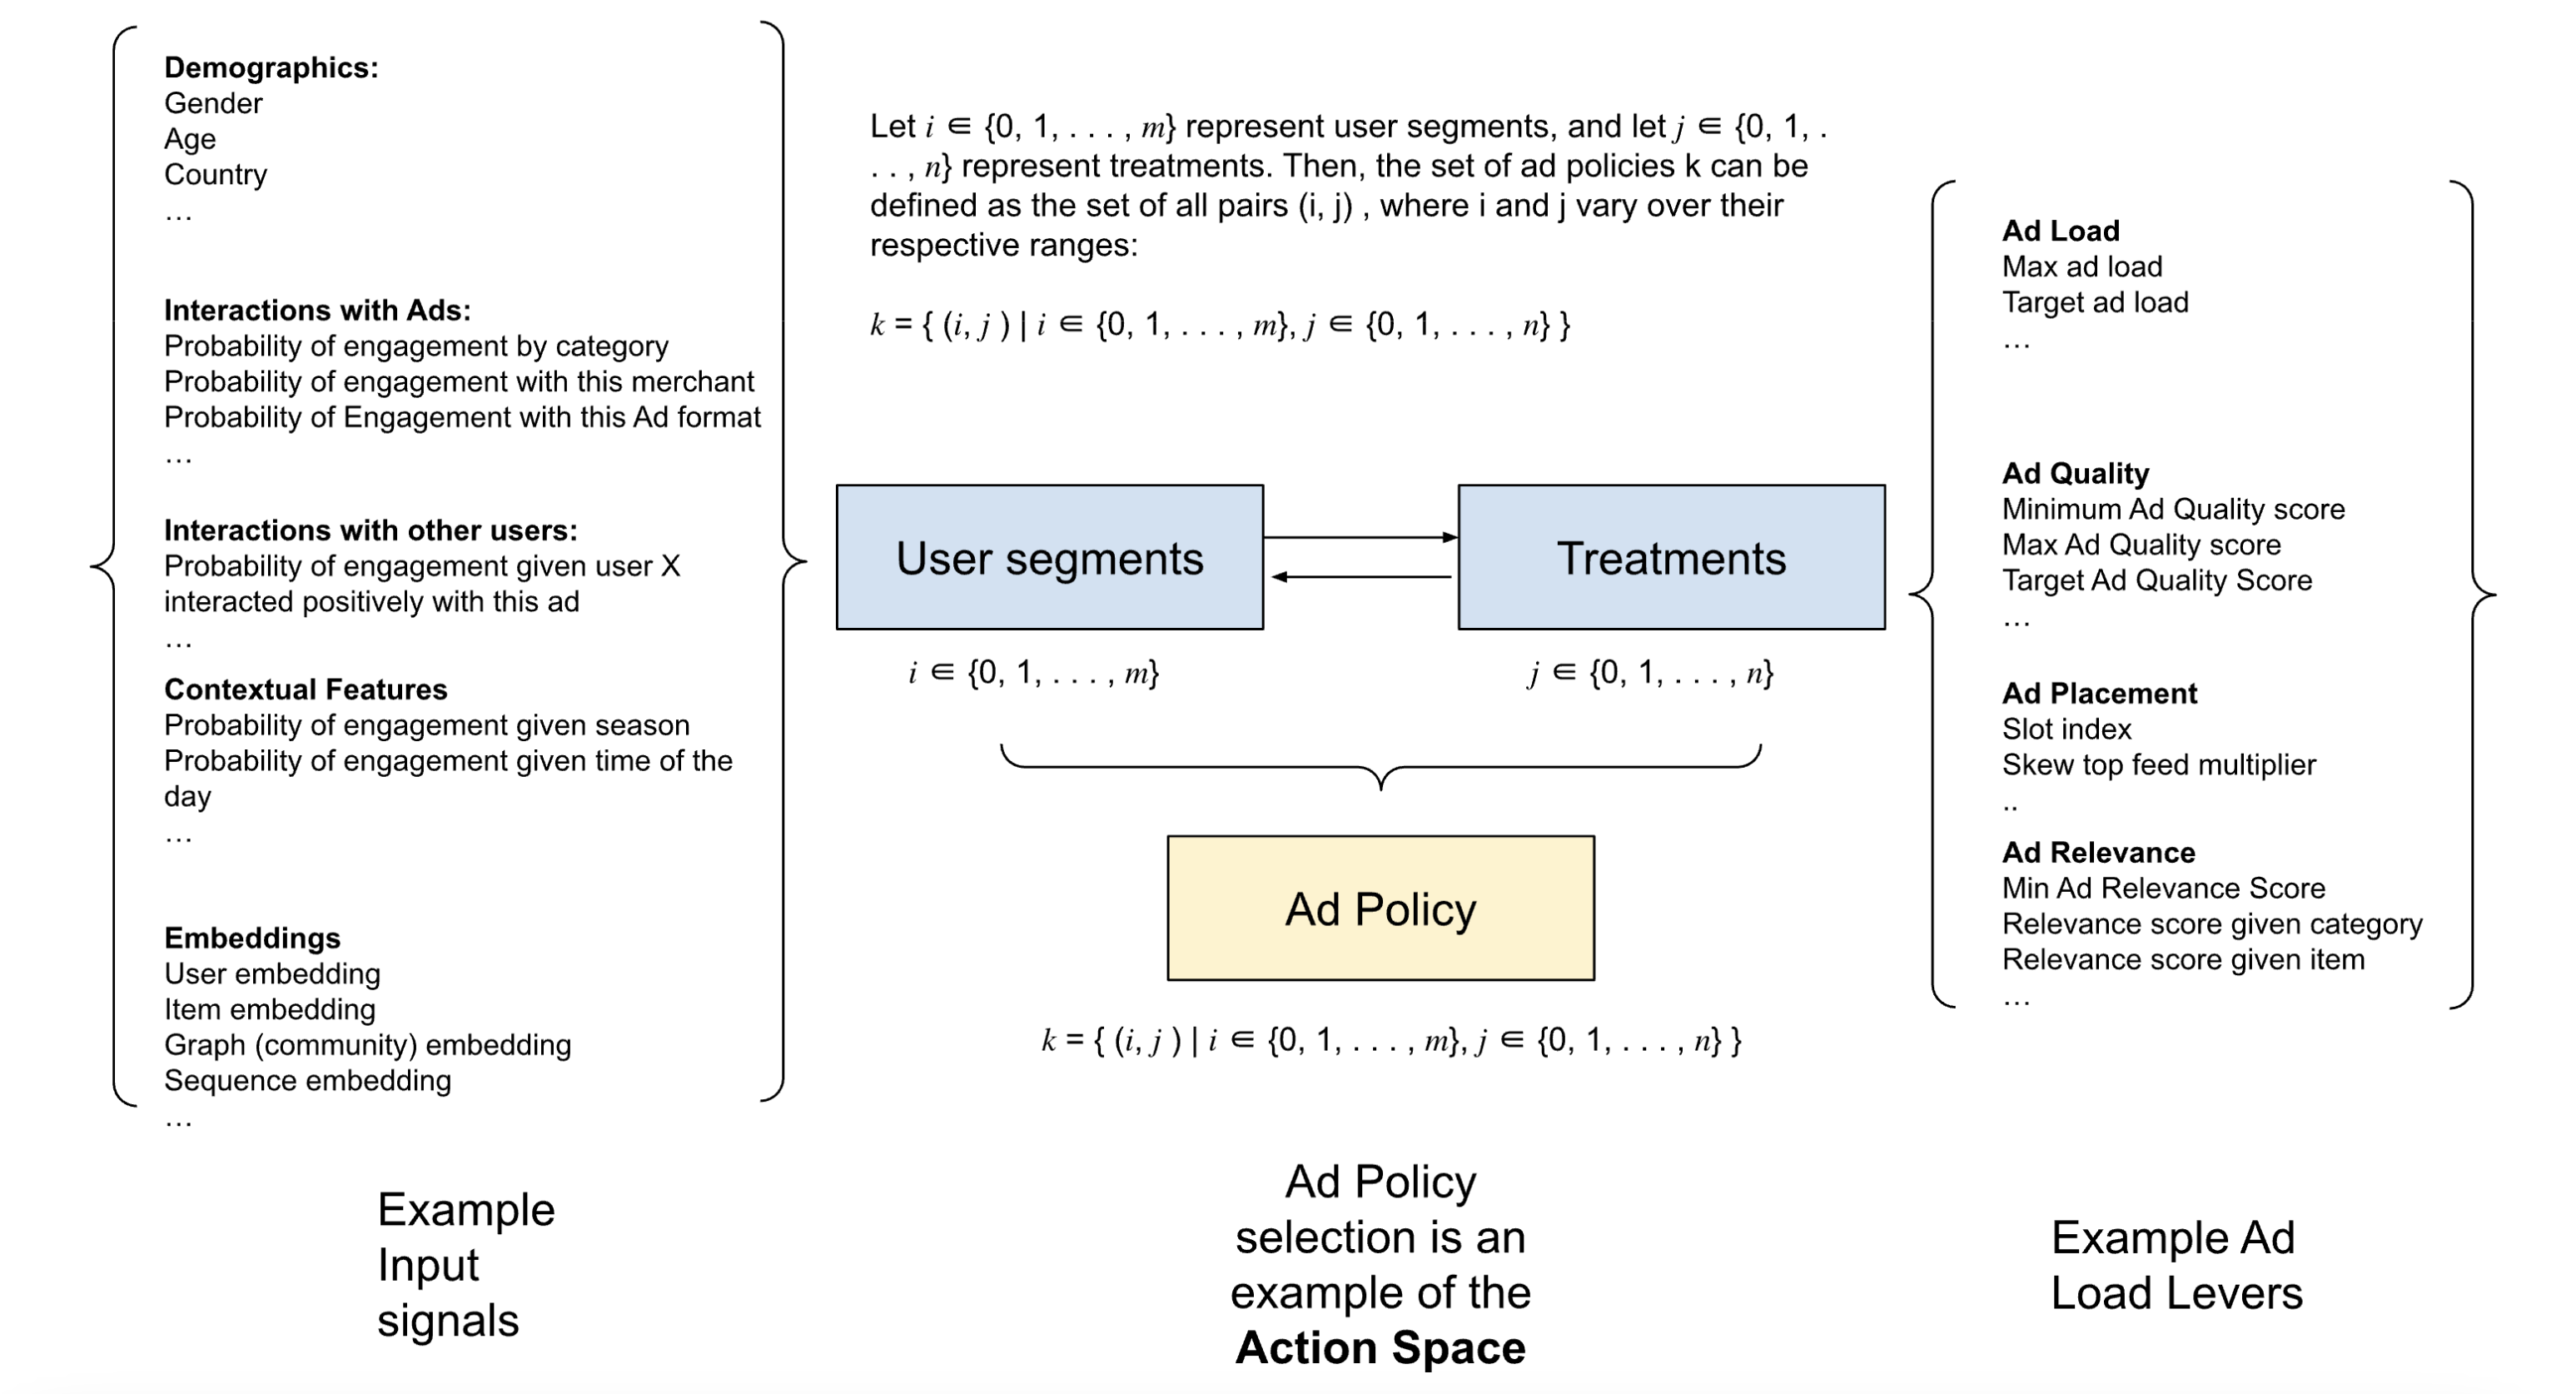
\includegraphics[width=\textwidth]{detailed_ad_policy.png}
    \caption{Example of an action set in the context of ad policies in recommendation systems}
    \label{fig:detailed_ad_policy}
\end{figure*}

\section{Conclusions}

The integration of RL in policy optimization for large-scale recommender systems has gained popularity as a promising approach to balance long-term and short-term objectives in environments with complex user behavior and revenue dynamics. However, scaling RL in practice presents challenges, including vast state and action spaces, reliance on proxy metrics, and significant computational demands. This paper provides an overview of effective, scalable techniques that address these challenges, offering insights into how RL can be applied at scale.
Unlike traditional methods that focus on optimizing short-term outcomes, RL’s cumulative reward framework enables it to account for both immediate and delayed feedback. Together, contextual bandits and offline replay offer scalable, interpretable solutions that approximate full RL while managing real-time constraints. Contextual bandits support selecting optimal actions within each interaction based on the current state, maximizing immediate rewards, which are typically proxy metrics of the true long-term reward. Offline replay complements this by enabling counterfactual learning: multiple treatments can be tested across randomized populations to evaluate causal effects, refining policies for diverse user segments.

Future research may focus on enhancing interpretability, refining reward functions, and exploring decentralized approaches to handle complex decision layers. These advancements will bring RL closer to fulfilling its potential in providing tailored, dynamic ad recommendations that align user satisfaction with business goals in large-scale recommendation systems.




\section*{Acknowledgements}
I would like to thank my advisor, Yuri Lawryshyn, for his valuable guidance and direction throughout this work. I also extend my gratitude to Adam Obeng, Bee-Chung Chen, and Jay Adams for their critical coaching and insights, which have significantly shaped my approach and understanding of industry practices. Their expertise has been key in aligning academic research with practical applications.

% This unnumbered section should be blank when submitting your paper. After review, you may include lists of people and organizations who supported the work.

% Print the biblography at the end. Keep this line after the main text of your paper, and before an appendix. 
% % THIS IS A LATEX TEMPLATE FILE FOR PAPERS INCLUDED IN THE
% *Anthology of Computers and the Humanities*. ADD THE OPTION
% 'final' WHEN CREATING THE FINAL VERSION OF THE PAPER. 
% DO NOT change the documentclass
%\documentclass[final]{anthology-ch} % for the final version
\documentclass[final]{anthology-ch}         % for the submission

% LOAD LaTeX PACKAGES
\usepackage{booktabs}
\usepackage{graphicx}
\usepackage{tabularx}
\usepackage{adjustbox}  % lets us make the table wider than \textwidth
\usepackage{setspace}
\usepackage{enumitem}
\usepackage{makecell}
% \usepackage{multirow}
\usepackage{float}

% \usepackage[table,xcdraw]{xcolor} % Allows the use of HTML colors

\addbibresource{bibliography.bib}


% \PassOptionsToPackage{table,xcdraw}{xcolor}


\geometry{
  a4paper,
  top=2cm,
  bottom=2cm,
  left=2cm,
  right=2cm
}

% ADD your own packages using \usepackage{}

% TITLE OF THE SUBMISSION
% Change this to the name of your submission
\title{A Review of Reinforcement Learning Applications in Ad Policy Optimization for Large-Scale Recommender Systems}

% AUTHOR AND AFFILIATION INFORMATION
% For each author, include a new call to the \author command, with
% the numbers in brackets indicating the associated affiliations 
% (next section) and ORCID-ID for each author.  
\author{Armando Ordorica}

\author{Yuri Lawryshyn}

% While we encourage including ORCID-IDs for all authors, you can
% include authors that do not have one by definining an empty ID.


% There should be one call to \affiliation for each affiliation of
% the authors. Multiple affiliations can be given to each author
% and an affiliation can be given to multiple authors. 
\affiliation{University of Toronto, Toronto, Canada}

% KEYWORDS
% Provide one or more keywords or key phrases seperated by commas
% using the following command

\keywords{Reinforcement Learning, Ad Policy Optimization, Contextual Bandits, Recommendation Systems,  Off-Policy Learning, Online Advertising, Deep Reinforcement Learning,  Multi-Objective Optimization}

% METADATA FOR THE PUBLICATION
% This will be filled in when the document is published; the values can
% be kept as their defaults when the file is submitted
\pubyear{2025}
\pubvolume{1}
\pagestart{1}
\pageend{1}
\conferencename{Proceedings of Conference XXX}
\conferenceeditors{Editor1 Editor2}
\doi{00000/00000}  

% \addbibresource{bibliography.bib}


\setstretch{2.0}

\begin{document}


\maketitle
% \doublespacing

\begin{abstract}
Balancing advertisements with organic content in large-scale recommendation engines is a well-known challenge in the industry. While ads are essential for revenue generation in platforms that integrate them alongside organic content, they often underperform in user engagement compared to organic content \cite{hochstein2023toward}. The key challenges in achieving this balance include ad selection, ranking, and integration with organic content. These involve decisions about whether to insert an ad, which ad to select, and where to place it \cite{zhao2020jointly}. Traditional methods optimize for the highest probability of ad clickthrough with fixed placements and are typically solved as supervised Machine Learning (ML) problems \cite{covington2016deep}. However, these approaches focus on optimizing single actions, overlooking the downstream impact of sequential user behavior and underutilizing valuable contextual signals. A more dynamic approach that accounts for context and optimizes the long-term value of action sequences, balancing both engagement and revenue, remains an open research area \cite{lin2023survey}.\\

Reinforcement Learning (RL) offers a promising framework to address the need for dynamic, context-aware optimization by formalizing the process of finding the best policy in sequential decision-making under uncertainty \cite{dimitrakakis2018decision}. However, implementing RL in large-scale recommendation systems faces challenges such as vast state and action spaces, the risk of poorly chosen reward functions, high computational costs \cite{pancha2022pinnerformer}, and the difficulty of interpreting online policy learning \cite{van2024practical}. This paper surveys existing methodologies and frameworks that utilize RL to enhance recommendation strategies, aiming to guide practitioners and researchers in navigating these challenges. Our analysis reveals that while fully online RL is powerful in theory, in practice, techniques like contextual bandits, offline replay, and surrogate reward modeling often yield more scalable and interpretable solutions for large-scale ad-serving.
\end{abstract}

% \tableofcontents

\section{Introduction}

Platforms such as Google, Meta, TikTok, and Pinterest offer content recommendation systems whose revenue models depend on an effective balance between advertisements and organic content \cite{zhao2020jointly} \cite{danescu2010competing}. This balance is essential to maximize immediate revenue while avoiding long-term issues such as ad fatigue, where users become less responsive to ads due to overexposure, and user churn, where users discontinue using the platform \cite{sagtani2023quantifying} \cite{silberstein2023combating}.\\

Over the past decade, deep learning has emerged as a promising technique that enables recommendation engines to better understand context through embeddings, significantly improving their ability to personalize content \cite{naumov2019deep} \cite{zhao2024survey}. However, deep learning approaches are often supervised and rely on measurable and observable short-term metrics used as model labels, such as the probability of a click-through or the likelihood of a video being watched in full \cite{nvidia_recommender_systems_2021}. Methodologies that use myopic objective functions to optimize these directly measurable short-term metrics often overlook the long-term value of a recommendation \cite{mazoure2021improving}. By focusing on immediate rewards, they may rank content based on short-term engagement metrics while neglecting the entire sequence of user interactions that involve delayed responses. Such approaches can result in suboptimal outcomes, such as promoting clickbait content that compromises long-term revenue and user engagement.\\

	% 4.	How does Reinforcement Learning (RL) offer a promising solution to these challenges?

To overcome the challenges of optimizing based solely on immediate objectives, Reinforcement Learning (RL), modeled as a Markov Decision Process (MDP), has emerged as a promising framework \cite{afsar2022reinforcement}. RL enables the consideration of long-term value by optimizing policies that maximize cumulative rewards over time, rather than focusing on short-term engagement metrics. In an MDP, actions are selected based on a policy ($\pi$), which chooses the action that maximizes the expected cumulative reward from the current state onward. This cumulative reward is typically conceptualized as the expected sum of future rewards, discounted over time using a discount factor. A lower discount factor places more emphasis on immediate rewards, effectively ignoring future outcomes. Conversely, a discount factor approaching one values future rewards more heavily, encouraging the policy to consider long-term benefits \cite{Sutton1998}. \\

In the context of recommendation systems, rewards can be defined to capture both user engagement and revenue objectives. Engagement rewards might include metrics such as time spent on the platform, content views, clicks, saves, shares, or likes \cite{wang2022surrogate}. Revenue rewards can be tied to ad-related metrics like ad impressions, ad clicks, conversions, or purchases resulting from ad exposure. These different rewards are often combined into a single utility function that reflects the platform’s overall objectives \cite{zhao2020jointly} \cite{zou2019reinforcement} \cite{xu2023optimizing}.\\

For example, the reward function  $r_t$  at time  $t$  can be defined as:

$$
r_t = \alpha \times \text{Engagement Metric}_t + \beta \times \text{Revenue Metric}_t,
$$ where  $\alpha$  and  $\beta$  are weighting factors that balance the importance of user engagement and monetization. By appropriately defining the utility function and choosing suitable weights, RL algorithms can optimize policies that enhance user experience while maximizing revenue over the long term \cite{zhao2020jointly, zhao2021dear, yan2020ads, sagtani2024ad}. \\


% What specific challenges are encountered when implementing RL in large-scale recommendation systems?
Despite the promising theoretical framework that RL offers for optimizing long-term value in recommendation systems, implementing RL in real-world, large-scale platforms remains complex \cite{dulac2021challenges}. First, in the context of recommendation systems, the state space, which reflects the current context of the user and the environment, and the action space, which captures how the recommender system can be tuned, are both essentially infinite \cite{zhu2021overview}. This vastness makes learning and optimization computationally intensive and difficult to discretize into individual actions and states, a critical requirement for policy learning \cite{afsar2022reinforcement} . \\ 

Second, designing appropriate reward functions is critical, as poorly chosen reward functions can lead to unintended system behaviors that degrade user experience or negatively affect business revenue \cite{everitt2021reward}. For example, a reward function that overly prioritizes click-based metrics may drive the system to promote clickbait content, boosting short-term engagement but eroding user trust and satisfaction over time \cite{wu2017returning}. Similarly, a reward function too heavily skewed toward revenue metrics could result in excessive ad load, disrupting the user experience and leading to churn. Striking the right balance in reward function design is essential to achieve both user engagement and monetization objectives without compromising the platform’s long-term goals.\\


Furthermore, interpretability is a major challenge in RL deployment. Understanding the learned policies--the strategies adopted by the RL agent--can be particularly difficult when policies are updated in real-time during user interactions (online policy learning) \cite{glanois2024survey} \cite{vouros2022explainable} \cite{dulac2019challenges}. This real-time adaptation complicates monitoring and evaluation, making it challenging to understand what is happening during online learning. In extreme cases, this lack of transparency could result in non-compliant or unethical behavior, posing significant risks to both users and the business \cite{lambert2023entangled}.\\

	% 7.	What are the objectives and contributions of this paper?
In light of the challenges outlined above, this paper examines methodologies and frameworks used to implement RL for large-scale recommendation systems, with a particular focus on contexts where ad revenue is central to the business model. Although previous surveys address RL in recommendation systems \cite{lin2023survey, afsar2022reinforcement}, they do not specifically explore how RL can balance the competing demands of ad and organic content. This paper fills that gap by analyzing approaches tailored to these unique challenges and bridging the divide between theoretical RL concepts and their real-world applications.
\\

The paper begins with a historical overview of ad selection and ranking systems, tracing the evolution from simple rule-based models and heuristic approaches to tree-based models and modern deep learning techniques. Each of these stages is explored in detail, highlighting their limitations and the motivations for adopting RL as the next paradigm in recommendation systems. Following this contextual history and motivation, the paper introduces key RL components such as the action space, state space, reward functions, and policies, using a straightforward toy example: the frozen lake problem. This example provides a foundation for understanding RL fundamentals, which are then mapped to real-world challenges in online advertising and recommendation systems. Drawing on these analogies, the paper offers a clear and practical framework to help practitioners navigate the implementation of RL and adapt these methodologies to their specific needs.


	% 8.	How will this paper help practitioners and researchers navigate the challenges of implementing RL in recommendation systems?


	% 13.	What is the structure of the paper, and what can readers expect in the subsequent sections?

\section{Paper Collection Methodology}

To ensure broad coverage, relevant papers were collected from both academic and industry sources. Foundational academic works such as \textit{Reinforcement Learning: An Introduction} \cite{Sutton1998}, \textit{Statistical Methods for Recommender Systems} \cite{agarwal2016statistical}, and \textit{Artificial Intelligence: A Modern Approach} \cite{russell2016artificial} were used to establish key mathematical foundations, including Markov Decision Processes (MDPs), Contextual Bandits, Off-Policy Learning, and Offline Replay.

To reflect the internal perspective of a production-facing ad policy team, a curated list of 10–15 papers referenced within Pinterest’s Ad Policy team was also compiled. Examples include \textit{Jointly Learning to Recommend and Advertise} \cite{zhao2020jointly}, \textit{DEAR: Deep Reinforcement Learning for Online Advertising Impressions in Recommender Systems} \cite{zhao2021dear}, \textit{Ad-load Balancing via Off-Policy Learning} \cite{sagtani2024ad}, and \textit{Practical Bandits} \cite{van2024practical}. In addition, targeted keyword searches such as “Reinforcement Learning ads [company name]” and “Contextual Bandit [company name]” were conducted for leading companies in the advertising and recommendation space (e.g., Google, Meta, Pinterest, Microsoft, TikTok, YouTube, LinkedIn),  surfacing additional papers describing real-world systems and methodologies. To complement those efforts, a separate search was conducted on Google Scholar for relevant review papers. While no surveys were found that specifically focused on RL in ad recommendation systems, related reviews on "contextual bandits", "ad fatigue", and "recommender systems" were used to identify additional references.

Finally, manual crawling of citation networks in cornerstone papers was used to identify additional key contributions. For instance, tracing citations from \textit{Jointly Learning to Recommend and Advertise} \cite{zhao2020jointly}, \textit{DEAR} \cite{zhao2021dear}, and \textit{Offline Reinforcement Learning} \cite{levine2020offline} led to works such as \textit{Ads Allocation in Feed via Constrained Optimization} \cite{yan2020ads} and \textit{A Contextual Bandit Bake-off} \cite{bietti2021contextual}.
In total, 153 papers were selected and reviewed. Papers were ranked according to three main criteria: influence, to capture the foundational or widely adopted ideas in the field; industry relevance, to ensure that the outcomes were sound, implementable, and actionable; and recency, to reflect the latest methodological developments and deployment practices.

While recent and highly cited work was prioritized, papers introducing novel methodologies were also included regardless of citation count. To contextualize the selected works, this survey builds from the ground up. Each component of the Markov Decision Process, including states, actions, rewards, and policies, is defined and illustrated using a toy example such as the Frozen Lake. This foundation is then extended to practice through a review of how each component is operationalized in industry, along with a discussion of the limitations of those approaches. Drawing on existing methods and lessons from industry, the resulting framework is intended to inform practitioners exploring how RL can be applied in their organizations to develop ad policies that balance monetization with organic engagement. A comparison between the toy example and real-world implementation parallels can be found in Table \ref{tab:comparison}.



\section{A Brief History of Ad Selection and Ranking in Recommendation Systems}

\begin{figure}[ht]
    \centering
    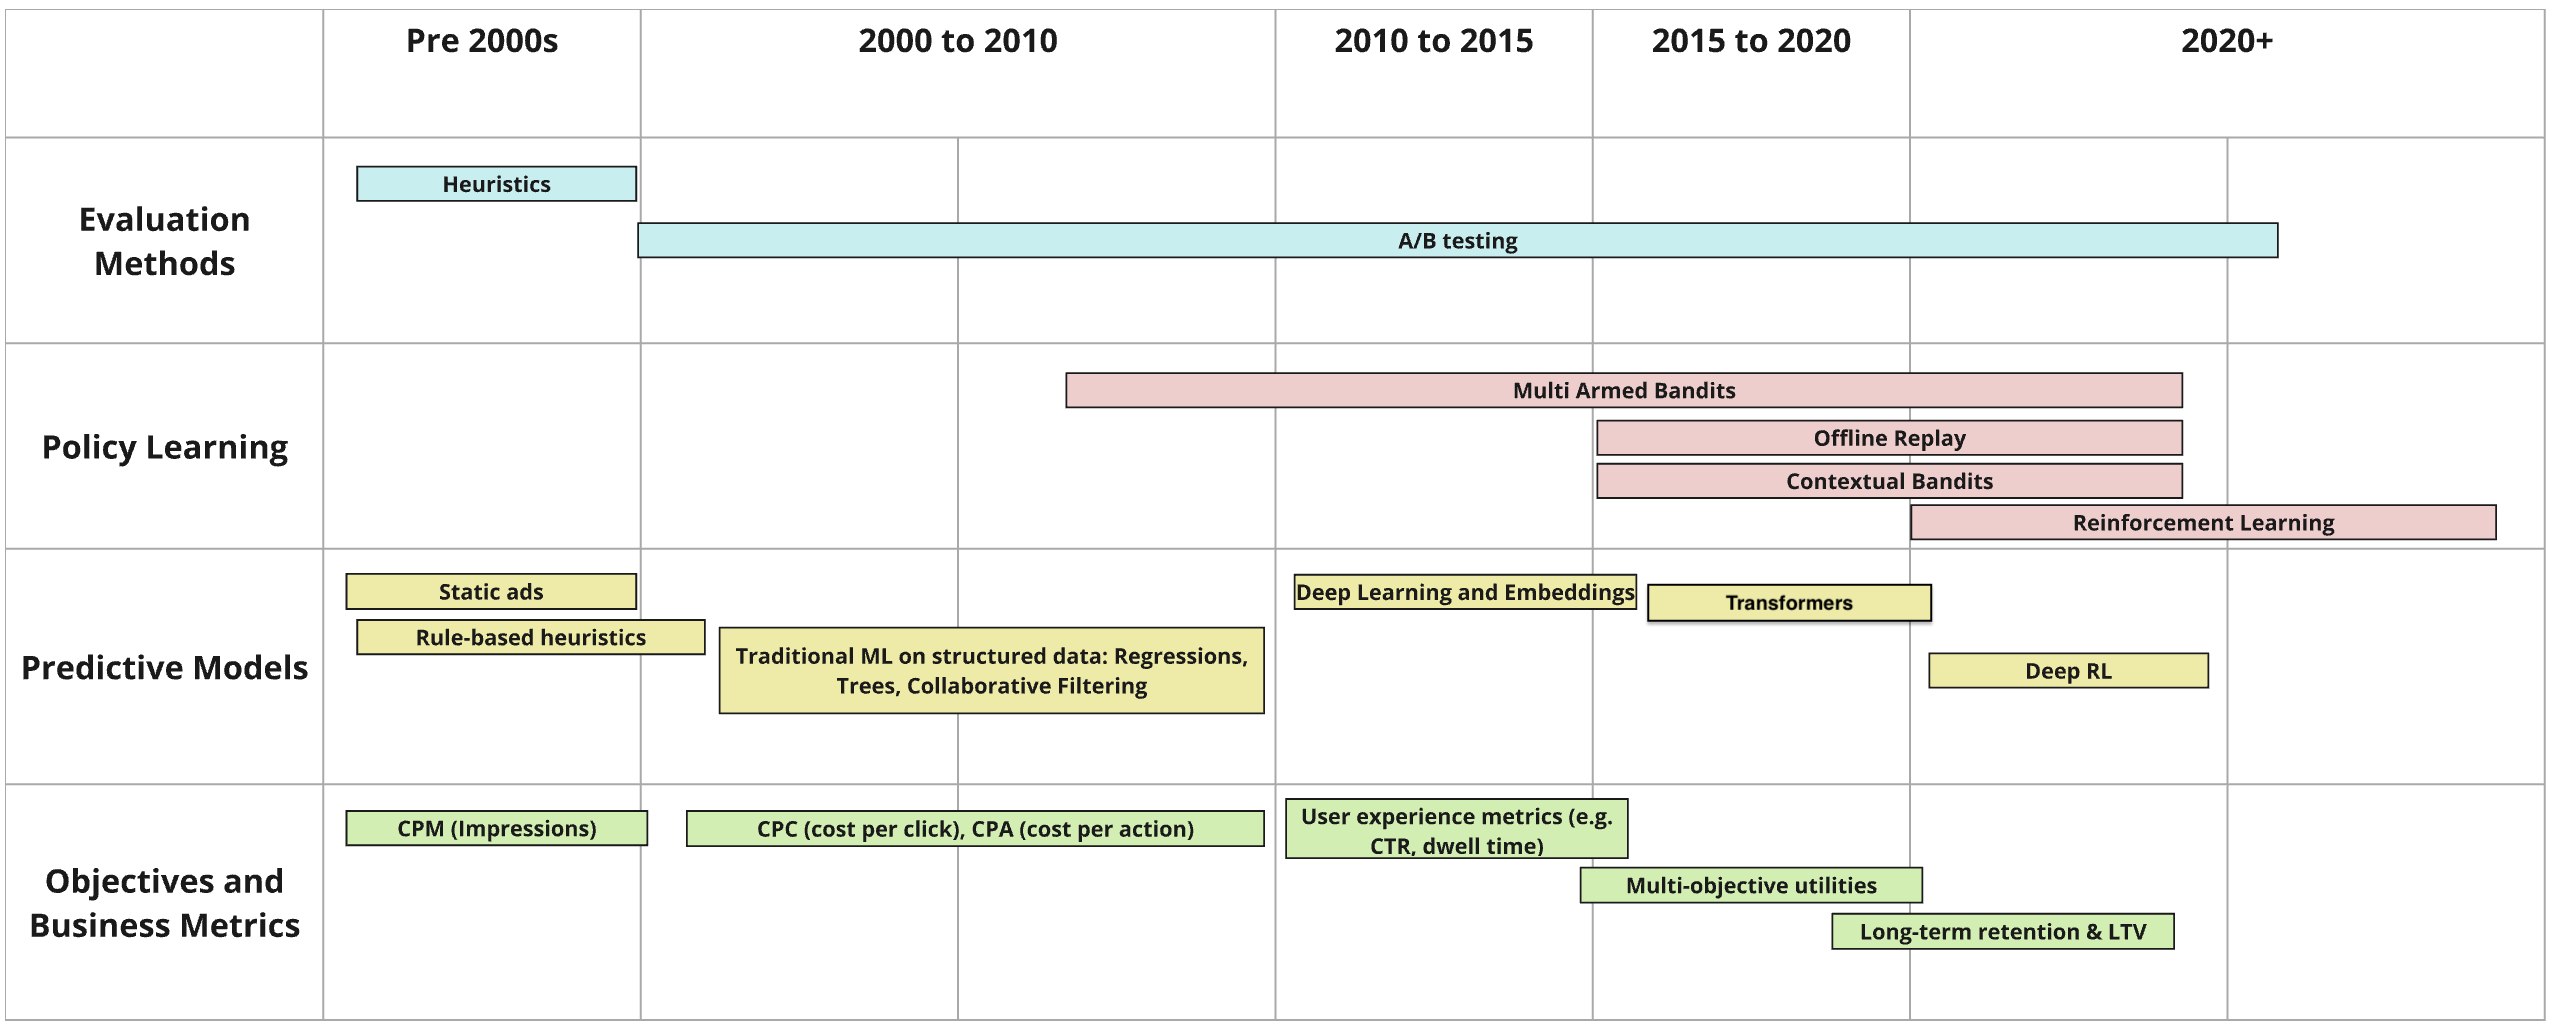
\includegraphics[width=\textwidth]{history_timeline_figure.png}
    \caption{Timeline Showing Initial Adoption and Popularization of Techniques and Methodologies in Online Advertising}
    \label{fig:ad_timeline}
    \vspace{0.2cm} % adds small vertical spacing
    \begin{flushleft}
        \footnotesize{\textit{Note:} The boundaries and lengths of rectangles are approximate. Innovations and transitions between techniques and objectives occurred gradually and continuously, rather than sharply at specific dates.}
    \end{flushleft}
\end{figure}


In online advertising, a good ad policy can result in positive revenue for the company while also boosting user experience. Conversely, a poor ad policy involves showing ads that are irrelevant to the user’s current intent, overloading the feed with excessive ad density, and failing to align content with the user’s interests. Irrelevant ad targeting can lead to ad fatigue, a state where users become desensitized or frustrated by excessive or poorly targeted ads, resulting in decreased engagement with both the ads and the platform as a whole \cite{ccelik2023ad}. \\

This section traces the evolution of advertising recommendation algorithms, culminating in the adoption of RL to overcome the limitations of earlier approaches. It begins by outlining how early online advertising primarily mirrored offline methods through banner ads and other static formats. It continues by explaining how static online advertising evolved over time to incorporate rule-based models and more sophisticated heuristic techniques. The discussion then transitions to the integration of machine learning methods, including regression-based models, tree-based algorithms, and collaborative filtering, followed by the emergence of deep learning and embedding-based approaches that effectively capture the nonlinear interactions between users and content. Finally, RL is introduced as a promising solution to address the shortcomings of preceding methodologies. This evolution is visually represented in Table \ref{fig:ad_timeline}, which shows the initial adoption and popularization of techniques and methodologies in online advertising. \\

\subsection{From Rule-Based Advertising to Traditional Machine Learning}
\textbf{Around the early 2000s, online advertising largely mirrored offline practices, heavily relying on non-targeted formats such as banner ads \cite{kant2021history}.} These generic advertising methods conflicted with the objective of search engines of efficiently directing users to relevant content \cite{fain2006sponsored}. As a marginal improvement on nontargeted ad formats like banner ads, advertisers began to utilize simple \texttt{if-then} logic with predefined rules to select and display ads based on basic criteria like user demographics. While rule-based systems were straightforward to implement, their lack of flexibility and personalization became evident as ad fatigue, defined as reduced user engagement due to repeated exposure to the same advertisement, persisted \cite{abrams2007personalized}. This issue underscored the necessity of not only leveraging user signals but also optimizing ad load tuning parameters, such as frequency and placement, to maintain user interest and maximize click-through rates \cite{abrams2007personalized}. For instance, researchers at LinkedIn introduced concepts like top slot - highest eligible position for an ad within the feed -  and minimum gap - the required distance between consecutive ads to prevent oversaturation - as ad load tuning parameters \cite{yan2020ads}. Their research indicated that users are more likely to click on ads that are spaced farther apart \cite{yan2020ads}. \\

\textbf{The evolution of ad pricing, from paying for impressions to paying for user actions, created pressure within the online advertising industry to improve relevance and performance-based metrics \cite{hu2004performance}.} Sponsored search, introduced by GoTo (later Overture), allowed advertisers to bid on specific keywords, directly linking ads to user queries and addressing the limitations of generic advertising  \cite{fain2006sponsored}. Foundational pricing models, such as Cost per Mille (CPM), charged advertisers per 1,000 impressions and closely mirrored offline practices \cite{wikipedia-cpm}. Yahoo!, through the acquisition of Overture \cite{wsj2003yahoooverture}, later introduced Cost per Click (CPC) \cite{ellam2003overture}, a performance-based pricing model that shifted costs to reflect measurable user engagement. This evolution continued with the introduction of Cost per Action (CPA), which tied fees to specific user actions beyond clicks, such as purchases or sign-ups. These changes incentivized the advertising industry to innovate, leading to the development of more relevance-focused strategies. These foundational pricing models remain integral to the utility functions that underpin contemporary ranking algorithms \cite{fain2006sponsored}. As advertisers increasingly demanded performance-based pricing, the ad tech industry was compelled to innovate within a competitive yet lucrative market, addressing the limitations of rule-based and heuristic models through the adoption of machine learning techniques to enable more dynamic and data-driven approaches \cite{zhang2018whole}.



\textbf{The next set of innovations following heuristics and performance-based targeting was led by machine learning (ML) and A/B testing \cite{barajas2022online}}. From 2010 to 2015, ad selection techniques evolved significantly with the adoption of machine learning models such as Logistic Regression, Decision Trees, and Gradient Boosting Machines \cite{cui2015global}. By leveraging historical data and diverse user behavior signals, these models enabled more accurate predictions of user engagement \cite{cui2015global}. In parallel, A/B testing allowed practitioners to systematically compare models and features, ensuring that any new implementation delivered measurable performance gains \cite{barajas2022online}.
Despite these successes, traditional tabular models struggled to capture nuanced user intent, particularly when processing more complex data such as images or text. In the early 2010s, deep learning gained momentum with breakthroughs like AlexNet \cite{krizhevsky2012imagenet}, which demonstrated the power of neural networks to handle unstructured high-dimensional data. This ability to capture complex, nonlinear interactions dramatically improved ad recommendations, especially through the use of embeddings, which are dense vector representations that map words or images into high-dimensional spaces. Metrics like cosine similarity further refined personalization by aligning recommendations with user interests \cite{covington2016deep}. Embedding-based models, particularly two-tower architectures, presented a major leap forward in ad recommendation systems by effectively capturing intricate relationships between users and ads. These models utilize two neural networks: one dedicated to encoding user information and the other to encoding ad (item) information. The outputs from these networks are then combined to predict user engagement with ads \cite{vorotilov2023scaling}. This approach not only boosted accuracy but also scaled effectively. Despite the significant improvements that embedding-based models introduced in terms of predictive accuracy and scalability of ad recommendation systems, the practical challenges of balancing multiple objectives, such as maximizing revenue, mitigating ad fatigue, and sustaining long-term user engagement remained unresolved.  


\textbf{Multi-Armed Bandits (MABs) emerged as a powerful method for online advertising around the 2010s to minimize user exposure to suboptimal ad configurations, effectively tackling the explore–exploit tradeoff, which consists of finding the optimal balance between choosing new ad policies with unknown performance and showing older ad policies with known positive performance \cite{schwartz2017customer} \cite{burtini2015improving}.} MABs are a class of algorithms for dynamic decision-making under uncertainty, originally developed in mid-20th-century probability theory \cite{robbins1952sequential}. While MABs had been widely applied in areas such as clinical trials \cite{villar2015multi} \cite{thompson1933likelihood}, they only gained significant traction in online advertising around the 2010s \cite{schwartz2017customer}.  

MABs allow platforms to reduce unnecessary exposure to a suboptimal treatment by continuously updating the probability distribution of which treatment is most likely to yield the highest reward \cite{kuleshov2014algorithms}. In clinical trials, for instance, a bandit algorithm reduces unnecessary exposure to suboptimal treatments by updating its reward estimates in real time: it allocates more patients to the better-performing treatment (exploitation) while still testing others that could be better (exploration) \cite{kuleshov2014algorithms}\cite{villar2015multi}. In this setting, the “reward” might be a measurable improvement in patient health or recovery time \cite{villar2015multi}. The same principle applies to online advertising, where “treatments” translate into specific ad configurations, defined by parameters such as displacement cost, reserve price, ad load, and ad placement. “Rewards” in online advertising typically represent user engagement metrics such as clicks or conversions \cite{schwartz2017customer}. Advertising platforms should continuously “explore” new treatments to test new ads, formats, and targeting strategies to avoid stagnation, while simultaneously “exploit” existing high-performing treatments to ensure near-term revenue targets are met \cite{schwartz2017customer}.  

In contrast to traditional A/B tests, where there are randomized treatments assigned for a predetermined amount of time, MABs dynamically learn which configuration yields the highest reward for each user at a particular time. This approach reduces the time users are exposed to suboptimal ad configurations, thereby mitigating losses in engagement and long-term revenue \cite{schwartz2017customer}. Although this dynamic learning framework effectively tackles the explore–exploit tradeoff, defining the precise set of rewards and objectives to optimize remains an open challenge, particularly when advertisers must juggle multiple goals such as revenue and long-term user satisfaction \cite{wen2019learning}.

\textbf{To address this need for clear, multi-objective definitions, such as balancing user satisfaction and revenue, utility functions have been employed in online advertising since the early 2000s \cite{engel2008incorporating}.} Rooted in microeconomic theory dating back to the mid-20th century, utility functions are mathematical constructs that quantify preferences and the net value of conflicting objectives \cite{Stigler1950} \cite{vonNeumannMorgenstern1944}. Introduced to formalize decision-making under uncertainty, they model and quantify consumer preferences, enabling advertisers and publishers to encode multiple objectives, such as revenue, user satisfaction, and long-term platform health, into a single or composite utility metric \cite{engel2008incorporating}. By integrating utility functions into MAB-based frameworks, advertisers can systematically guide the exploration–exploitation process toward a unified reward signal that balances short-term performance (e.g., clicks, impressions, or conversions) with long-term considerations (e.g., minimizing ad fatigue or maintaining user trust). This approach allows for principled trade-offs, optimizing for immediate gains while safeguarding long-term engagement.


\subsection{Advances in Deep Learning: Attention Models, Transformers, and Contextual Bandits}

\textbf{While embedding-based models greatly enhanced the predictive power of recommendation systems, capturing the full complexity of user sequences, especially over long time spans, remained a challenge for sequential deep learning methods such as  Long Short-Term Memory networks (LSTMs) and Gated Recurrent Units (GRUs) \cite{vaswani2017attention} \cite{gao2024mamba}.} Traditional recurrent networks (e.g., LSTMs or GRUs) process sequences step by step, typically encoding an entire sequence into a single fixed-size vector \cite{Sutskever2014}. This design poses several challenges. Because Recurrent Neural Networks (RNNs) operate strictly in a sequential manner, they cannot process multiple parts of the sequence in parallel, creating bottlenecks and risking the loss or blurring of details, especially those from earlier steps in long sequences \cite{vaswani2017attention}.  Moreover, standard RNNs inherently prioritize recent inputs as information is passed along, which attenuates earlier signals and leads to the well-known vanishing gradient problem in lengthy sequences and fails to effectively capture long-term dependencies \cite{Bengio1994}\cite{Pascanu2013}. 


\textbf{To address training inefficiencies in RNNs and the difficulty of capturing long-term dependencies, attention mechanisms allow direct access to any position in the sequence, enabling the model to focus on relevant features in the sequence regardless of their temporal distance \cite{vaswani2017attention}. }By computing pairwise interactions across all positions in the sequence, Transformers overcome the sequential bottlenecks of RNNs and enable parallel computation \cite{vaswani2017attention}.  This mechanism also allows the model to incorporate contextual signals, such as user demographics, session-level metadata, or item attributes, at any point in the sequence, rather than strictly depending on a running hidden state \cite{kang2018sasrec}. The ability to attend to any part of the input at any time allows Transformers to model long-range dependencies with far greater efficiency and accuracy than RNN-based architectures \cite{vaswani2017attention}. This paradigm shift led to the development of the Transformer architecture, which entirely replaces recurrence with self-attention, fundamentally redefining sequence modeling \cite{vaswani2017attention}.

\textbf{The Transformer’s parallel attention architecture is a natural fit for modern hardware.} Since self-attention and feed-forward layers are implemented with large matrix operations, the model makes efficient use of Graphics Processing Units (GPUs) and Tensor Processing Units (TPUs), which excel at parallel computation \cite{vaswani2017attention}. Unlike RNNs that left many GPU cores underutilized due to their step-by-step nature, Transformers keep the hardware busy by processing many elements concurrently. This yields significantly shorter training times compared to earlier recurrent models. Moreover, Transformers scale up seamlessly: training can be distributed across multiple GPUs, and larger batches or longer sequences can be handled without a drop in throughput \cite{shim2022comparison}. Engineers can simply add more GPU workers to accommodate bigger models or more data, achieving near-linear speedups in many cases \cite{brown2020language}. The ability to train deep models efficiently at scale has unlocked previously impractical projects, and Transformer-based architectures (e.g. BERT, GPT) are now standard building blocks in modern AI systems \cite{brown2020language} \cite{kaplan2020scaling}. One of the key innovations of the Transformer architecture is its multi-head attention mechanism \cite{vaswani2017attention}. Instead of relying on a single attention distribution, multiple attention “heads” are trained in parallel, each with its own set of learned parameters. This design allows the model to capture a range of relationships or patterns within the same sequence \cite{vaswani2017attention}.In practice, each head can focus on different aspects. One head might emphasize local dependencies in the user’s interaction history, while another one might highlight more global, long-range correlations \cite{vaswani2017attention}.


\textbf{In an advertising context, multi-head attention naturally accommodates multi-objective learning \cite{ma2018modeling}.} For example, one head could be tuned to prioritize short-term engagement metrics (e.g., click-through rate or CTR) by attending to recent user activities and relevant ad features, while another head could emphasize longer-term outcomes, such as mitigating ad fatigue or preserving user satisfaction \cite{zhao2019recommending} \cite{ma2018modeling}. Each head learns a distinct set of attention weights, enabling the model to isolate and capture unique signals that serve different goals \cite{an2024tmh}. The outputs from these multiple heads are then aggregated, typically concatenated and linearly transformed, into a single representation or score, providing a unified but multi-faceted embedding of user–ad interactions \cite{vaswani2017attention} \cite{lyu2023entire}. However, determining the appropriate attention heads and their optimal weighting remains a complex challenge \cite{vaswani2017attention}\cite{Kang2018} \cite{Voita2019}. The optimal weights may vary not only across different users and content types but also over time \cite{Zhou2018} \cite{Zhou2019}. Additionally, shifting business objectives, engineering constraints, and competing optimization objectives further complicate the design process \cite{Mehrotra2018} \cite{Mehrotra2020} \cite{Jannach2023}. 

%How is head selection and weighing typically done 
\textbf{Selecting the right heads in Multi-Task Attention Models and determining their optimal weighting is not a deterministic process \cite{Michel2019} \cite{Voita2019}.} It typically requires iterative experimentation, involving both offline analysis (e.g., hyperparameter tuning, head ablation studies) and online testing (A/B experiments) \cite{Michel2019} \cite{kang2018sasrec}. This process is particularly challenging for new users and new content, where slow adaptation can result in suboptimal personalization and early churn \cite{Schein2002, Bobadilla2013}. 

%tie this up to Offline Replay 
\textbf{To address difficulties related to policy optimization - like weight tuning and head selection - \textit{Offline Replay} is often employed to find optimal policies in large parameter search spaces  \cite{agarwal2016statistical} \cite{levine2020offline} \cite{agarwal2020optimistic}.} This technique typically begins with data collection via A/B/n experiments, where different policies are randomly assigned to users \cite{agarwal2019online} \cite{chen2009large}. Afterward, Offline Replay simulates the effects of various ad policies across different user segments and estimates the potential rewards based on logged interactions \cite{agarwal2016statistical}. In this context, “reward” refers to the performance metric we aim to maximize (i.e. clicks, likes, shares, revenue) \cite{wu2017returning}. However, in many cases, the true optimal treatment is not explicitly tested \cite{agarwal2019online}. Here, importance sampling corrects for differences between the observed behavior policy and the target policy, improving estimation accuracy \cite{Sutton1998} \cite{dudik2011doubly}.  Based on the collected data on random assignments between policies and users typically involved in Offline Replay, one can use different policy learning methods to map the optimal policies from user ids, content types, and other contextual signals for the optimal weights at any point in time \cite{swaminathan2015counterfactual}. 


%  As a form of counterfactual learning, it estimates potential rewards under different policies by simulating outcomes based on logged interactions. This enables the system to learn from sparse or delayed feedback and serves as a critical tool for safely testing new policies offline \cite{sagtani2024ad}.\\

% In this context, “reward” refers to the performance metric we aim to maximize. For example, a click or any other positive action on an item is considered a reward. Sometimes, a positive action like a click can be weighted by a downstream utility, such as advertising revenue or time spent on a landing page (the page displayed after a user clicks on a recommended item), to derive a weighted reward. Our goal is to estimate the expected reward of a new ad policy using data collected in the past \cite{agarwal2016statistical}.\\

\textbf{Offline replay  often assumes that user preferences and item availability do not change significantly during data collection. }However, in real ad systems, these factors can shift, causing offline data to become stale or biased \cite{levine2020offline} \cite{agarwal2014taming}. Contextual bandits address this limitation by leveraging continuous feedback from live user interactions, preventing the policy from being locked into a static offline dataset \cite{li2010contextual}. Contextual bandits can be thought of as a special case of RL, where an action selection does not influence future states \cite{bubeck2012regret} \cite{Sutton1998}. Unlike full RL, which models long-term state transitions, contextual bandits assume that each decision is independent, optimizing for immediate rewards rather than a multi-step trajectory \cite{bubeck2012regret} \cite{Sutton1998}. This makes them particularly well-suited for recommender systems, where ranking decisions can be treated as independent events \cite{afsar2022reinforcement} \cite{zhou2016latent}. Additionally, contextual bandits naturally balance exploration and exploitation, allowing them to adapt dynamically to user behavior in real time \cite{li2010contextual}. However, a practical limitation of contextual bandits is that they select actions from a fixed set defined at deployment time, such as preconfigured ad policies or treatment arms \cite{bietti2021contextual}. As a result, the policy’s performance is inherently constrained by the quality and granularity of the available states and actions at the time of inference \cite{dimitrakakis2018decision}.

\textbf{Although contextual bandits inherently focus on short-term rewards, they can be tuned to approximate long-term objectives by encoding historical or delayed outcomes into the feature space or the immediate reward function \cite{mcdonald2023impatient} \cite{wu2017returning}.} For instance, if an attention head emphasizing ad engagement indirectly correlates with better retention, a contextual bandit can increase its weight over time, provided that retention signals are reflected in the contextual features or the reward proxy \cite{yi2023progressive}. However, full RL remains more appropriate for scenarios demanding explicit multi-step optimization, where actions taken now significantly shape future user states \cite{gauci2018horizon}. Contextual bandits thus offer a practical trade-off, providing continuous adaptation and efficient online learning without the computational complexity of fully modeling multi-step state transitions \cite{gauci2018horizon} \cite{levine2020offline}.


\textbf{Despite the practical advantages that contextual bandits offer for real-time experimentation and short-horizon reward maximization, they remain limited in scenarios where user states evolve over repeated interactions \cite{Sutton1998}.} Modern advertising platforms often contend with extended user sessions and multiple recurring visits, demanding an approach capable of modeling multi-step feedback loops. RL naturally extends these capabilities by incorporating stateful dynamics and cumulative rewards, capturing phenomena like ad fatigue \cite{ccelik2023ad} and long-term retention \cite{wu2017returning}. Recent industrial deployments underscore RL’s growing importance in ads: ByteDance uses RL-based systems \cite{zhao2020jointly,zhao2021dear} to balance immediate revenue with session-level engagement in short-video feeds, Meta (Facebook) has leveraged policy-gradient methods for sequencing notifications and ad placements over evolving user states \cite{gauci2018horizon}, and companies like Google are experimenting with RL-driven ad scheduling that accounts for shifting user contexts at scale \cite{zhao2024survey}. These efforts demonstrate how RL can transcend the myopic focus of bandits to address long-horizon outcomes, multi-objective trade-offs, and dynamic user behaviors. In the sections that follow, we explore how these RL paradigms are integrated into large-scale advertising stacks, focusing on core algorithms, design decisions, and lessons learned from real-world implementations.



\section{The RL formulation of the Ad Recommendation Problem}

In RL, the \textbf{GridWorld problem }is a foundational example of a Markov Decision Process (MDP), where an \textbf{agent} interacts with a \textbf{deterministic environment} by performing \textbf{discrete actions}, such as moving up, down, left, or right, to navigate through a grid with the objective of reaching a goal, while potentially avoiding obstacles or hazards. A more complex variant is the \textbf{FrozenLake problem}, which features a \textbf{stochastic environment} where movements are uncertain due to a slippery surface (\textcolor[HTML]{1E90FF}{F}) as shown in Figure~\ref{tab:frozen_lake} \cite{FrozenLakeGymnasium2023}. Here, \textbf{actions do not always lead to the intended next state}, adding complexity by requiring policies that effectively manage uncertainty. In this paper, \textbf{we use the FrozenLake problem as a representative framework for stochastic environments and leverage this template to describe the ad optimization problem as an RL task}. Specifically, we will explore components of the underlying MDP, such as states, actions, and rewards, and investigate key RL concepts including policy evaluation, value iteration, and policy iteration. The grid is typically represented as shown in Figure~\ref{tab:frozen_lake}:


\label{frozen_lake}


\begin{figure}[ht]
\centering
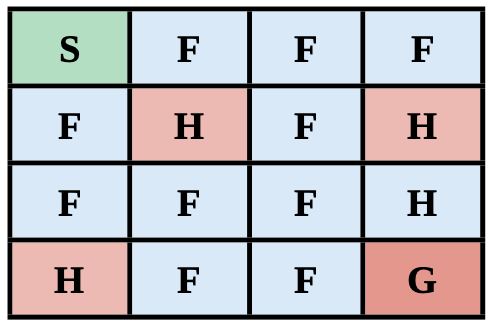
\includegraphics[width=0.35\linewidth]{frozenlake-table.png}
\caption{Frozen Lake Environment Grid}
\label{tab:frozen_lake}
\end{figure}


% \begin{table}[ht]
%     \centering
%     \setlength{\arrayrulewidth}{0.5mm}
%     \setlength{\tabcolsep}{12pt}
%     \renewcommand{\arraystretch}{1.5}
%     \begin{tabular}{|c|c|c|c|}
%         \hline
%         \cellcolor[HTML]{A9DFBF}\textbf{S} & \cellcolor[HTML]{D6EAF8}\textbf{F} & \cellcolor[HTML]{D6EAF8}\textbf{F} & \cellcolor[HTML]{D6EAF8}\textbf{F} \\ \hline
%         \cellcolor[HTML]{D6EAF8}\textbf{F} & \cellcolor[HTML]{F5B7B1}\textbf{H} & \cellcolor[HTML]{D6EAF8}\textbf{F} & \cellcolor[HTML]{F5B7B1}\textbf{H} \\ \hline
%         \cellcolor[HTML]{D6EAF8}\textbf{F} & \cellcolor[HTML]{D6EAF8}\textbf{F} & \cellcolor[HTML]{D6EAF8}\textbf{F} & \cellcolor[HTML]{D6EAF8}\textbf{H} \\ \hline
%         \cellcolor[HTML]{F5B7B1}\textbf{H} & \cellcolor[HTML]{D6EAF8}\textbf{F} & \cellcolor[HTML]{D6EAF8}\textbf{F} & \cellcolor[HTML]{F1948A}\textbf{G} \\ \hline
%     \end{tabular}
%     \caption{Frozen Lake Environment Grid}
%     \label{tab:frozen_lake} % This label is used to reference the table
% \end{table}


\begin{table*}[ht]
    \centering
    \small
    \begin{tabular}{|>{\centering\arraybackslash}p{3cm}|p{3.5cm}|p{9cm}|}
        \hline
        \textbf{Component of Markov Decision Process Formulation} & \textbf{Frozen Lake Example} & \textbf{Large Scale Recommendation Systems for Ad Policy Optimization} \\ 
        \hline
        \textbf{Environment} & The frozen lake. & The users. \\ 
        \hline
        \textbf{Goal} & Reach the goal (G) from the start position (S) while avoiding holes (H). The agent must avoid falling into a hole, and reaching the goal faster is rewarded. & Maximize revenue without compromising user experience. \\ 
         \hline
          \textbf{Episode} & A game. & A time period (T), typically 2 weeks, corresponding to an A/B experiment where enough data is collected to evaluate policy performance across users. \\ 
        \hline
        \textbf{Rewards} & Rewarded for reaching the goal (i.e., +100), but penalized for delays (i.e., -1 per step). & 
        The reward is typically represented by a utility function, which could be a weighted sum of metrics like user engagement (clicks, time spent) and revenue generated (ad clicks, conversions). The challenge lies in balancing short-term revenue with long-term user retention. \\ 
        \hline
        \textbf{Agent} & The learner. & The Recommendation System. \\ 
        \hline
        \textbf{Actions} & Up, down, left and right. & 
        Basically infinite. But when it comes to ad recommendations specifically, some typical actions are the following: 
        \begin{itemize}
            \item Reserve Price Floor: The minimum price at which an ad impression is sold.
            \item Displacement Cost Threshold: A measure of the opportunity cost for showing an ad.
            \item Max Ad Load: The maximum number of ads that can be shown without reducing user satisfaction.
            \item Ad Quality Thresholds: Standards used to ensure ads meet a quality bar before being shown.
            \item Ad Placement: The specific position of ads within the user feed (e.g., first, third, or fifth position).
        \end{itemize} \\
        \hline
        \textbf{States} & All possible grid positions the agent can occupy, representing the state space of the environment. & 
        \textbf{Signals}:
        \begin{itemize}
            \item User Context: Demographics, user profile
            \item Interaction Data: Previous interactions with ads, organic content
            \item Contextual Features: Time of day, browsing context
            \item Embeddings: Latent feature representations of user interests or ad features
        \end{itemize} \\
        \hline
        \textbf{Policy} & A mapping of grid positions to optimal action to take for a maximum reward. & 
        A mapping of user segments to ad treatments to maximize both revenue and user experience. This policy can be dynamically adjusted based on real-time feedback or offline simulations. \\ 
        \hline
    \end{tabular}
    \caption{Comparison of Frozen Lake Example and Large-Scale Recommendation Systems for Ad Policy Optimization}
    \label{tab:comparison}
\end{table*}

\subsection{The Agent and its Objective}
While toy examples like GridWorld \cite{Sutton1998}  and Frozen Lake \cite{frozenlake} provide well-defined, relatively simple environments where RL algorithms can be easily tested, transitioning these insights to real-world recommendation systems is far more complex due to factors like vast state–action spaces and delayed rewards, and environment observability \cite{dulac2019challenges, kaelbling1996reinforcement}. \textbf{Observability refers to the degree to which an agent can directly perceive the complete state of the environment} \cite{kaelbling1998planning}. In fully observable settings (such as the FrozenLake), the agent sees the true state at every step, enabling straightforward decision-making \cite{kaelbling1998planning}. However, real-world environments, including \textbf{recommendation systems, are often partially observable \cite{lu2016partially}}; the agent must infer the underlying state from incomplete or noisy signals, increasing both the computational complexity of learning and the uncertainty of policy outcomes \cite{wu2021partially}. In the FrozenLake environment, the \textbf{agent is a decision-maker that observes its surroundings and chooses actions}. It learns to navigate the grid to reach the goal (\textcolor[HTML]{FF4500}{G}) from the start position (\textcolor[HTML]{228B22}{S}) while avoiding holes (\textcolor[HTML]{FF0000}{H}) and navigating slippery surfaces (\textcolor[HTML]{1E90FF}{F}). By analogy, in ad policy optimization, \textbf{the agent is the algorithm responsible for serving ads}, which must balance two primary \textbf{objectives}: maximizing revenue while maintaining (or ideally enhancing) user engagement \cite{Theocharous-2015, zou2019reinforcement}. Ultimately, both the FrozenLake agent and the ad-serving algorithm share the same high-level goal: to maximize long-term rewards through strategic actions grounded in observed states.

The use of a \textbf{reward signal} to formalize the idea of a goal is a distinctive feature of RL \cite{Sutton1998}. In an MDP, the reward is a scalar value the agent receives after taking an action in a given state and transitioning to a new state, serving as immediate feedback on the benefit or cost of the action \cite{kaelbling1996reinforcement}. This feedback allows the agent to learn a policy that maximizes the cumulative reward over time \cite{kaelbling1996reinforcement}. In simple RL scenarios, rewards are typically straightforward. For instance, the agent might receive -1 per move (to encourage shorter paths), +100 for reaching the goal (G), and -100 if it falls into a hole (H), ending the episode. \textbf{However, in real-world recommendation systems, reward structures can be far more nuanced.  It is often unclear which user behaviors warrant the highest reward or how to weigh different signals} \cite{mcdonald2023spotify}. In online advertising, for example, low-intent actions such as clicks may be valued less than high-intent actions like saves or purchases. Moreover, deciding how to balance these varied signals in a single reward function can be both subjective and complex, especially when multiple objectives (e.g., revenue, user satisfaction, and content diversity) must be optimized \cite{mcdonald2023spotify}.\\

Ad recommendation engines often need to \textbf{balance multiple objectives}, such as maximizing user engagement while also ensuring ad revenue \cite{zhang2018whole, yan2020ads, sagtani2024ad}. Long-term engagement and revenue are metrics that are particularly difficult to measure directly, especially in randomized controlled experiments that typically span only a couple of weeks \cite{mcdonald2023spotify}. The delay in outcomes (e.g., retention signals may take months to manifest) and the often subtle impact of a single intervention can make it nearly impossible to detect meaningful changes within such short time frames \cite{mcdonald2023spotify}.  As a result, proxy metrics are commonly used. For instance, click-through rate (CTR) and ad impressions serve as approximate measures of revenue, while session duration, saves, and shares act as proxies for longer-term engagement \cite{wang2022surrogate}. However, these simpler proxies can fail to capture the system’s true long-term objectives, occasionally leading to suboptimal policies \cite{mazoure2021improving}. A high CTR may reflect short-term engagement, yet it can ultimately induce ad fatigue or frustrate users if the ads are misaligned with their actual interests \cite{hohnhold2015focusing, sagtani2024ad}. Table \ref{fig:proxy-metrics} summarizes some of the most commonly used proxies in the industry across dimensions of revenue, engagement, and ad fatigue. 


% \begin{figure}[H]
% \centering
% 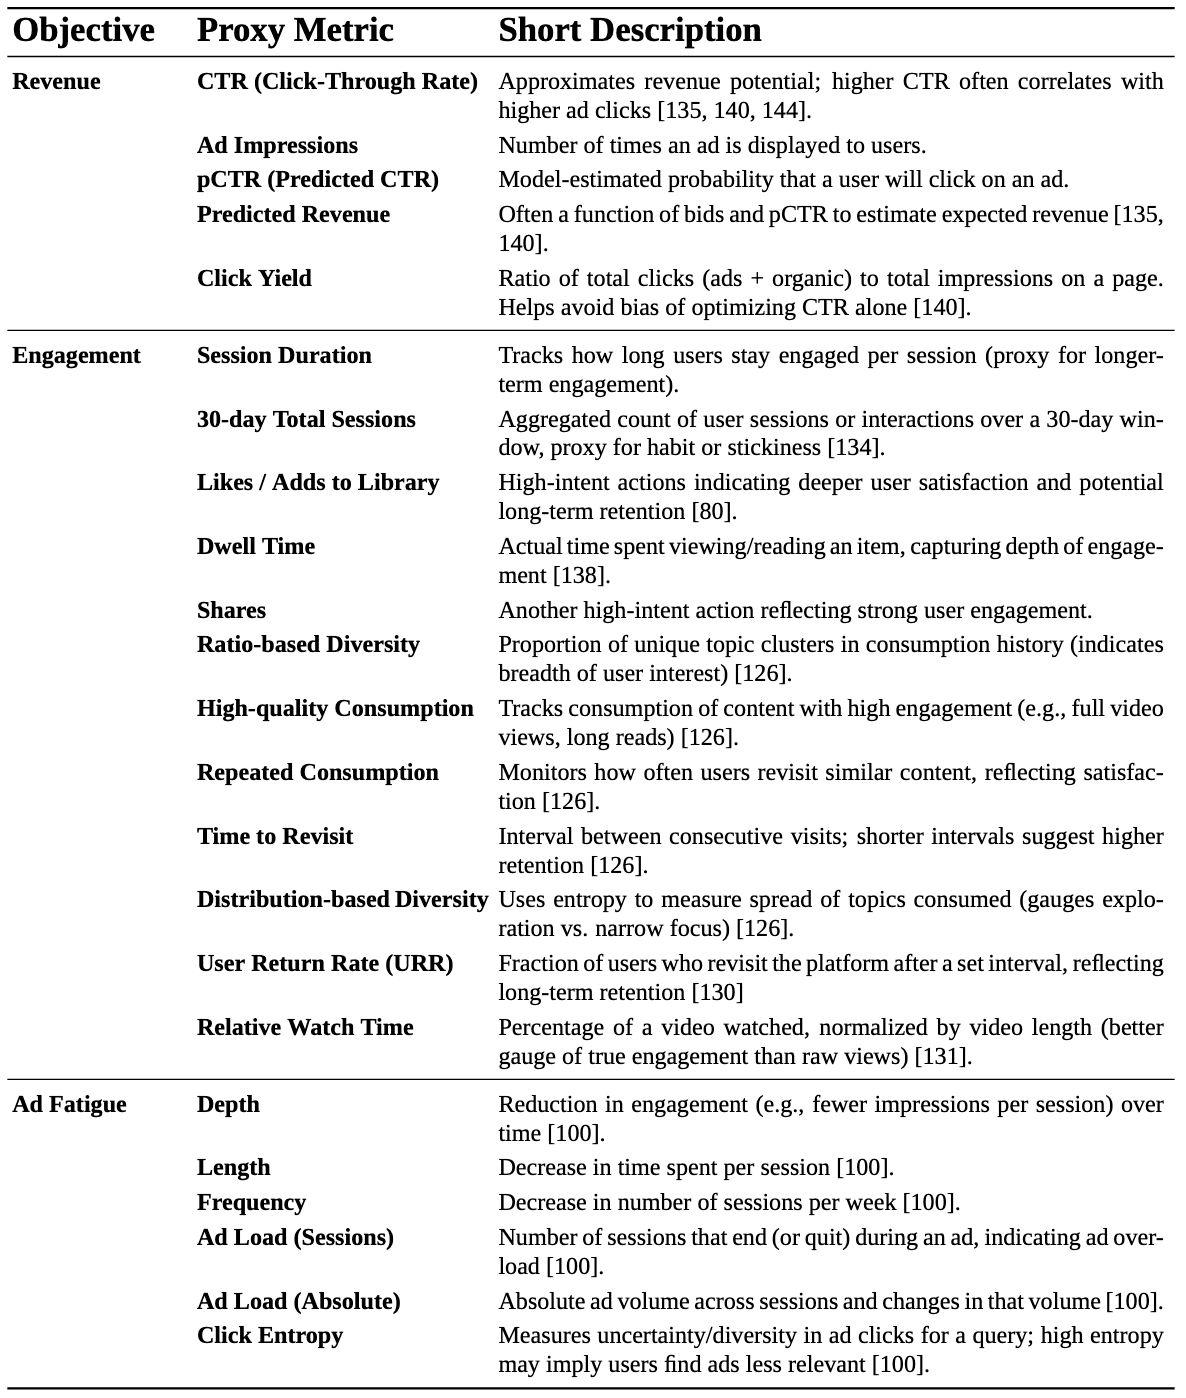
\includegraphics[width=\linewidth]{proxy-metrics-table.png}
% \caption{Proxy metrics for Revenue, Engagement, and Ad Fatigue.}
% \label{fig:proxy-metrics}
% \end{figure}

\begin{figure}[ht]
  \centering
  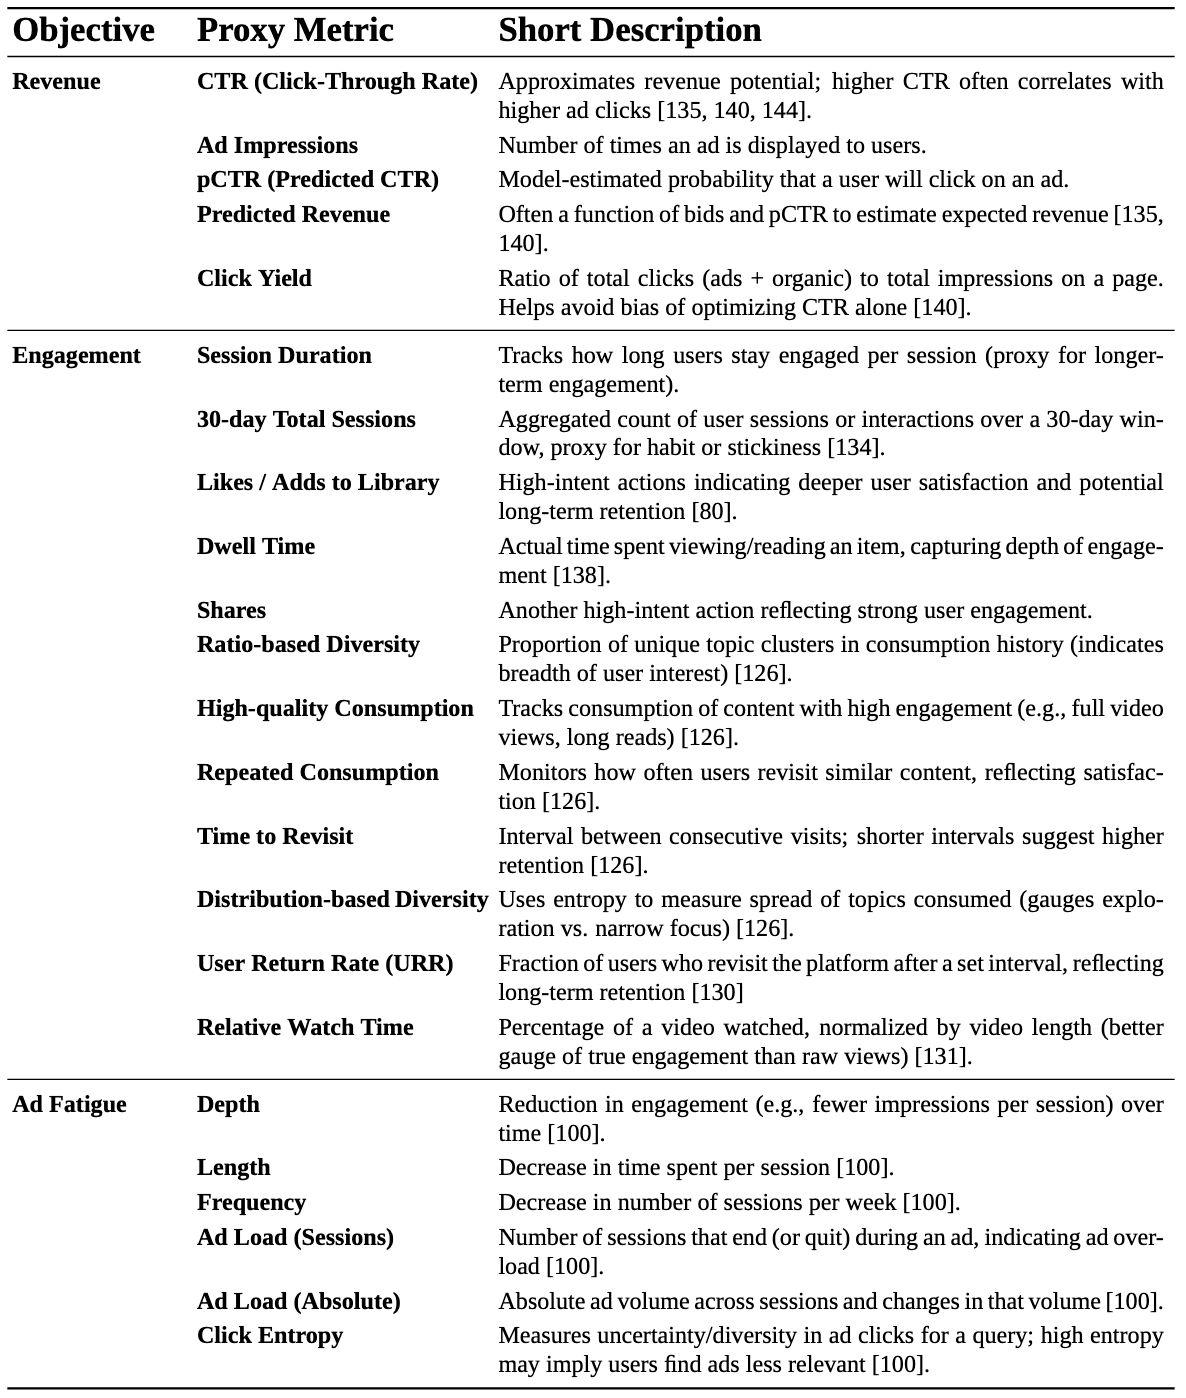
\includegraphics[width=\textwidth, height=0.85\textheight, keepaspectratio]{proxy-metrics-table.png}
  \caption{Proxy metrics for Revenue, Engagement, and Ad Fatigue.}
  \label{fig:proxy-metrics}
\end{figure}


% \begin{table}[H]
% \setstretch{1} % Ensure normal spacing within table. Separation between lines of the same cell. 
% \centering
% \small
% \renewcommand{\arraystretch}{1.2}  % Tweak if needed
% \setlength{\tabcolsep}{2pt} % separation between columns 
% \begin{tabularx}{\linewidth}{p{0.15\linewidth} p{0.25\linewidth} p{0.57\linewidth}}
% % the decimal points allow to control the size of the table, not of the text.
% \toprule
% {\bfseries \Large Objective} & {\bfseries \Large Proxy Metric} & {\bfseries \Large Short Description} \\
%   % \textbf{Objective} & \textbf{Proxy Metric} & \textbf{Short Description} \\
% \midrule
%     \multirow{\textbf{Revenue}} 
%        & \textbf{CTR (Click-Through Rate)} 
%            &  Approximates revenue potential; higher CTR often correlates with higher ad clicks \cite{zhang2018whole, yan2020ads, zhao2020jointly}. \\
%        & \textbf{Ad Impressions} 
%            & Number of times an ad is displayed to users. \\
%        & \textbf{pCTR (Predicted CTR)} 
%            & Model-estimated probability that a user will click on an ad. \\
%        & \textbf{Predicted Revenue} 
%            & Often a function of bids and pCTR to estimate expected revenue  \cite{yan2020ads, zhang2018whole}. \\
%        & \textbf{Click Yield} 
%            & Ratio of total clicks (ads + organic) to total impressions on a page. Helps avoid bias of optimizing CTR alone \cite{zhang2018whole}. \\
%     \midrule
%     \multirow{\textbf{Engagement}} 
%        & \textbf{Session Duration} 
%            & Tracks how long users stay engaged per session (proxy for longer-term engagement). \\
%         & \textbf{30-day Total Sessions} 
%        & Aggregated count of user sessions or interactions over a 30-day window, proxy for habit or stickiness 
%        \cite{xu2023optimizing}. \\
%        & \textbf{Likes / Adds to Library} 
%        & High-intent actions indicating deeper user satisfaction and potential long-term retention \cite{mcdonald2023spotify}. \\
%           & \textbf{Dwell Time} 
%        & Actual time spent viewing/reading an item, capturing depth of engagement  \cite{yi2014beyond}. \\
%        & \textbf{Shares} 
%            & Another high-intent action reflecting strong user engagement. \\
%     & \textbf{Ratio-based Diversity}  
%            & Proportion of unique topic clusters in consumption history (indicates breadth of user interest) \cite{wang2022surrogate}. \\
%        & \textbf{High-quality Consumption} 
%            & Tracks consumption of content with high engagement (e.g., full video views, long reads) \cite{wang2022surrogate}. \\
%      & \textbf{Repeated Consumption}  
%            & Monitors how often users revisit similar content, reflecting satisfaction \cite{wang2022surrogate}. \\
%               & \textbf{Time to Revisit} 
%            & Interval between consecutive visits; shorter intervals suggest higher retention \cite{wang2022surrogate}. \\
%      & \textbf{Distribution-based Diversity}  
%            & Uses entropy to measure spread of topics consumed (gauges exploration vs. narrow focus) \cite{wang2022surrogate}. \\
%     & \textbf{User Return Rate (URR)} 
%        & Fraction of users who revisit the platform after a set interval, reflecting long-term retention  \cite{wu2017returning} \\
%      & \textbf{Relative Watch Time} 
%        & Percentage of a video watched, normalized by video length (better gauge of true engagement than raw views) 
%       \cite{wu2018beyond}. \\
%     \midrule
%     \multirow{\textbf{Ad Fatigue}} 
%        & \textbf{Depth} 
%            & Reduction in engagement (e.g., fewer impressions per session) over time \cite{sagtani2023quantifying}. \\
%        & \textbf{Length} 
%            & Decrease in time spent per session \cite{sagtani2023quantifying}. \\
%        & \textbf{Frequency} 
%            & Decrease in number of sessions per week \cite{sagtani2023quantifying}. \\
%        & \textbf{Ad Load (Sessions)} 
%            & Number of sessions that end (or quit) during an ad, indicating ad overload \cite{sagtani2023quantifying}. \\
%        & \textbf{Ad Load (Absolute)} 
%            & Absolute ad volume across sessions and changes in that volume \cite{sagtani2023quantifying}. \\
%        & \textbf{Click Entropy} 
%            & Measures uncertainty/diversity in ad clicks for a query; high entropy may imply users find ads less relevant \cite{sagtani2023quantifying}. \\
% \bottomrule
% \end{tabularx}
% \caption{Proxy metrics for Revenue, Engagement, and Ad Fatigue.}
% \label{tab:proxy-metrics}
% \end{table}




\textbf{Utility functions are mathematical constructs used to estimate the net value of conflicting objectives \cite{Stigler1950}.} A utility function is a \textbf{composite reward function} that allows the agent to integrate various rewards or metrics from multiple objectives using a unified currency, facilitating more nuanced decision-making across competing priorities \cite{Stigler1950}. The ability to compare two utilities, like those of revenue and engagement normalized to a common scale, is critical for any principled blending of organic items and ads \cite{yan2020ads}.  Most utility functions are linear though this linearity is not a requirement for how the individual utility of each component is calculated \cite{wen2019learning, zhao2020jointly}. 

A \textbf{canonical utility function} at the policy layer to \textit{blend} ads and organic content can be represented as follows \cite{sagtani2024ad, yan2020ads, carrion2021blending}:
    \begin{equation}
        U(x) = \alpha \times \text{Revenue} + \beta \times \text{Engagement} - \gamma \times \text{Ad Fatigue}
    \end{equation}
    where $\alpha$, $\beta$, and $\gamma$ are weights that determine the relative importance of each factor. To compute the utilities of "Revenue", "Engagement", and "Ad Fatigue", typically many signals feed into each component. These signals include, but are not limited to, the ones shown in Table \ref{fig:proxy-metrics}. In a bandit or RL context, $U(x)$ serves as the reward signal guiding policy updates. The process of tuning the weights of $\alpha$, $\beta$, and $\gamma$ is often done through experimentation, as the right balance between engagement and revenue can shift depending on the context. For instance, ByteDance uses a multi-objective reward framework in their recommendation systems, where different reward functions are designed for organic content and ads, combining them to guide the overall recommendation strategy \cite{zhao2020jointly}.
    
In some cases, a very simple unified function can suffice over a complex utility function. Researchers at Alibaba introduced the concept of Click Yield, which is defined as the ratio of the total number of clicks on all items (ads + organic results) to the total number of impressions on a page \cite{zhang2018whole}. Click Yield provides a holistic evaluation of page performance, accounting for the interactive effects between ads and organic content, and helping to mitigate the bias that arises from examining CTR in isolation. Their optimization task maximizes total revenue while ensuring that the Click Yield does not fall below a certain threshold (T)  \cite{zhang2018whole}. A comparison of utility function formulations is shown in Table \ref{fig:utility-comparison}.

\begin{figure}[ht]
\centering
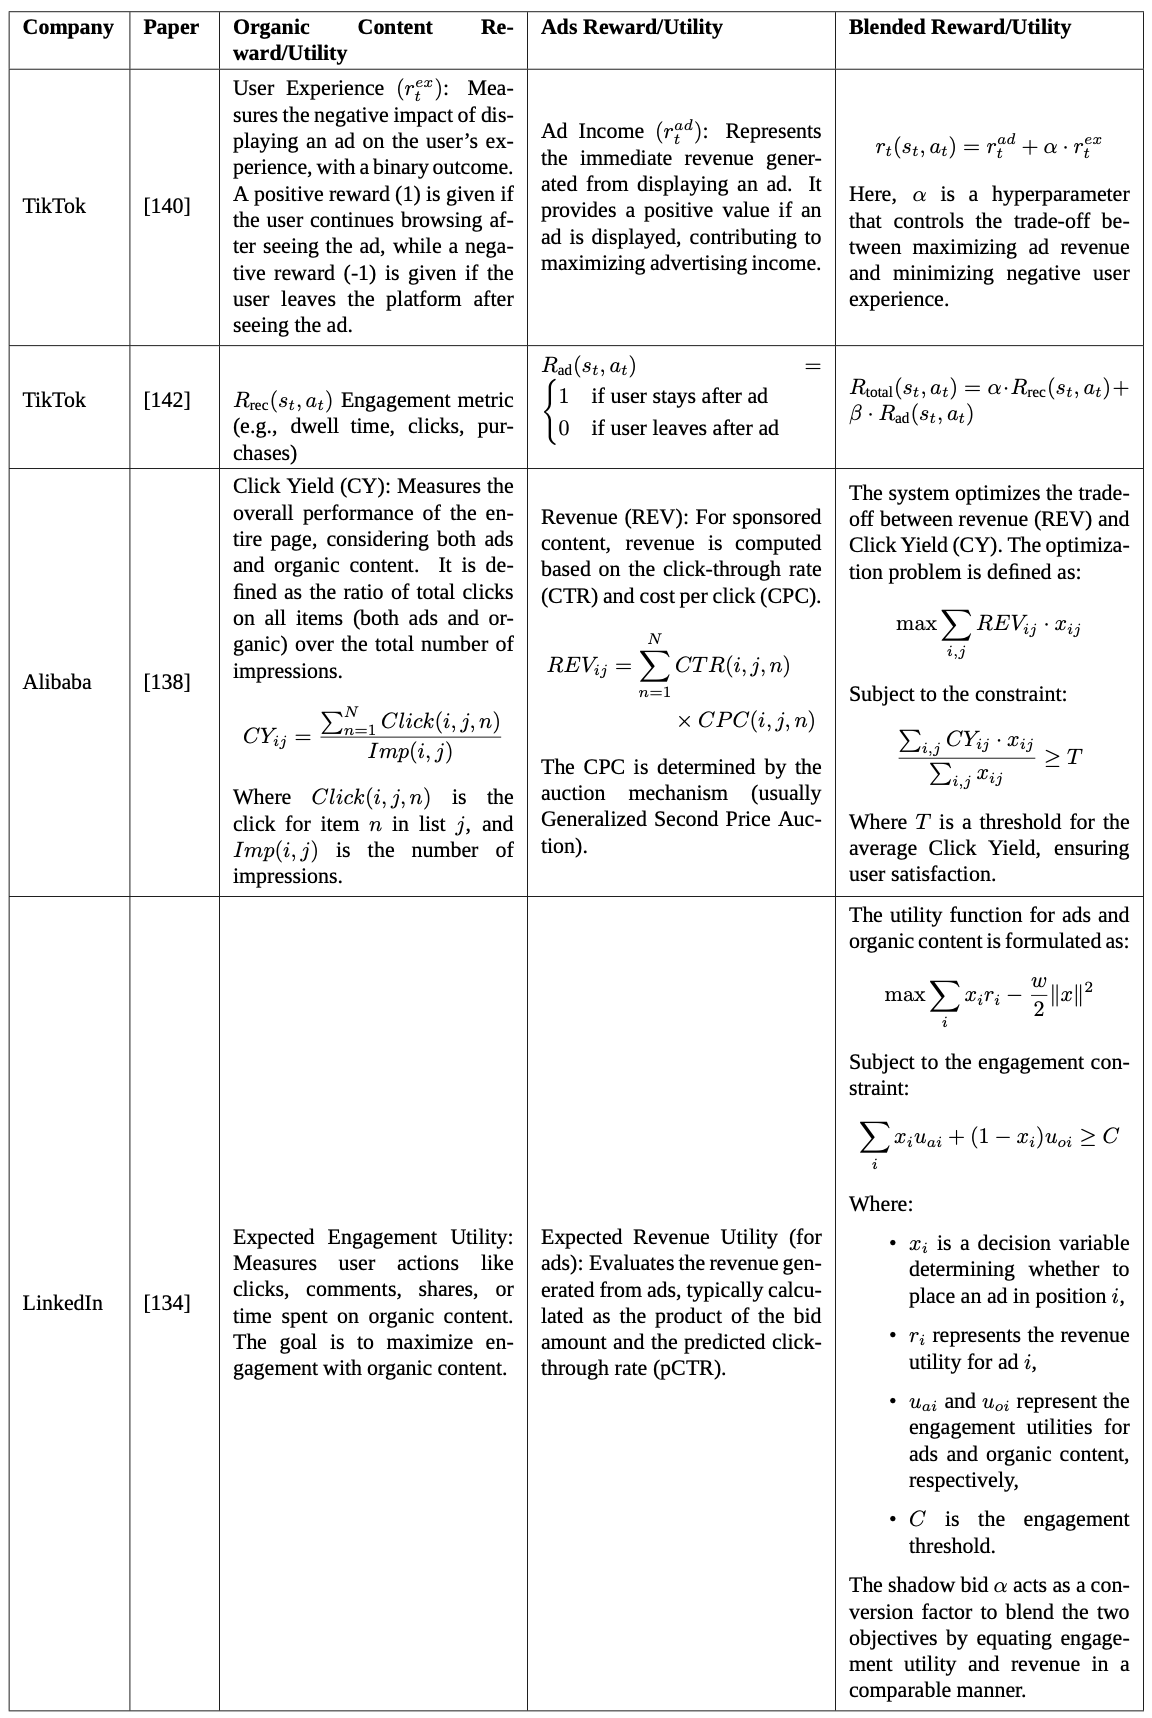
\includegraphics[width=\textwidth, height=0.85\textheight, keepaspectratio]{utility-comparison-table.png}
\caption{Comparison of Utility/Reward Formulation Approaches across Different Companies}
\label{fig:utility-comparison}
\end{figure}



% Adjusted table with better column width control and proper spacing
% \begin{table}[ht]
%     \centering
%     % \renewcommand{\arraystretch}{1.3}  % Adjust row height spacing
%     \begin{adjustbox}{max width=\textwidth}
%     \small % Decrease font size for the table
%     % \setlength{\tabcolsep}{6t} % Increase spacing between text and vertical lines
%     \renewcommand{\arraystretch}{1.15}
% \begin{tabular}{|p{1.5 cm}|p{1 cm}|p{4.5 cm}|p{4.5 cm}|p{4.5 cm}|}
%     \hline
%     \textbf{Company} & \textbf{Paper} & \textbf{Organic Content Reward/Utility} & \textbf{Ads Reward/Utility} & \textbf{Blended Reward/Utility} \\ 
%     \hline
%     TikTok & \cite{zhao2021dear} & 
%     \begin{minipage}{4.5cm}
%     \vspace{4pt}
%         User Experience \((r_t^{ex})\): Measures the negative impact of displaying an ad on the user's experience, with a binary outcome. A positive reward (1) is given if the user continues browsing after seeing the ad, while a negative reward (-1) is given if the user leaves the platform after seeing the ad.
%         \vspace{4pt}
%     \end{minipage}
%     & 
%     \begin{minipage}{4.5cm}
%     \vspace{4pt}
%         Ad Income \((r_t^{ad})\): Represents the immediate revenue generated from displaying an ad. It provides a positive value if an ad is displayed, contributing to maximizing advertising income.
%         \vspace{4pt}
%     \end{minipage}
%     & 
%     \begin{minipage}{4.5cm}
%     \vspace{4pt}
%         \[
%         r_t(s_t, a_t) = r_t^{ad} + \alpha \cdot r_t^{ex}
%         \]
%         Here, \(\alpha\) is a hyperparameter that controls the trade-off between maximizing ad revenue and minimizing negative user experience.
%         \vspace{4pt}
%     \end{minipage} \\
%     \hline
%     TikTok & \cite{zhao2020jointly} & 
%     $R_{\text{rec}}(s_t, a_t)$ Engagement metric (e.g., dwell time, clicks, purchases)  
%     & 
%     \begin{minipage}{4.5cm}
%     \vspace{4pt} 
%     \( R_{\text{ad}}(s_t, a_t) = 
%     \begin{cases} 
%         1 & \text{if user stays after ad} \\
%         0 & \text{if user leaves after ad} 
%     \end{cases} \) 
%         \vspace{4pt}
%     \end{minipage}
%     & 
%     \begin{minipage}{4.5cm}
%     \vspace{4pt}
%     \( R_{\text{total}}(s_t, a_t) = \alpha \cdot R_{\text{rec}}(s_t, a_t) + \beta \cdot R_{\text{ad}}(s_t, a_t) \)
%         \vspace{4pt}
%     \end{minipage} \\
%     \hline
%     Alibaba & \cite{zhang2018whole} & 
%     \begin{minipage}{4.5cm}
%     \vspace{4pt}
%         Click Yield (CY): Measures the overall performance of the entire page, considering both ads and organic content. It is defined as the ratio of total clicks on all items (both ads and organic) over the total number of impressions.
%         \[
%         CY_{ij} = \frac{\sum_{n=1}^{N} Click(i, j, n)}{Imp(i, j)}
%         \]
%         Where \(Click(i, j, n)\) is the click for item \(n\) in list \(j\), and \(Imp(i, j)\) is the number of impressions.
%         \vspace{4pt}
%     \end{minipage}
%     & 
%     \begin{minipage}{4.5cm}
%     \vspace{4pt}
%         Revenue (REV): For sponsored content, revenue is computed based on the click-through rate (CTR) and cost per click (CPC).
%         \[
% \begin{aligned}
% REV_{ij} = \sum_{n=1}^{N} & \, CTR(i, j, n) \\
% & \times CPC(i, j, n)
% \end{aligned}
% \]
%         The CPC is determined by the auction mechanism (usually Generalized Second Price Auction).
%         \vspace{4pt}
%     \end{minipage}
%     & 
%     \begin{minipage}{4.5cm}
%     \vspace{4pt}
%         The system optimizes the trade-off between revenue (REV) and Click Yield (CY). The optimization problem is defined as:
%         \[
%         \max \sum_{i,j} REV_{ij} \cdot x_{ij}
%         \]
%         Subject to the constraint:
%         \[
%         \frac{\sum_{i,j} CY_{ij} \cdot x_{ij}}{\sum_{i,j} x_{ij}} \geq T
%         \]
%         Where \(T\) is a threshold for the average Click Yield, ensuring user satisfaction.
%         \vspace{4pt}
%     \end{minipage} \\
%     \hline
%     LinkedIn & \cite{yan2020ads} & 
%     \begin{minipage}{4.5cm}
%     \vspace{4pt}
%         Expected Engagement Utility: Measures user actions like clicks, comments, shares, or time spent on organic content. The goal is to maximize engagement with organic content.
%         \vspace{4pt}
%     \end{minipage}
%     & 
%     \begin{minipage}{4.5cm}
%     \vspace{4pt}
%         Expected Revenue Utility (for ads): Evaluates the revenue generated from ads, typically calculated as the product of the bid amount and the predicted click-through rate (pCTR).
%         \vspace{4pt}
%     \end{minipage}
%     & 
%     \begin{minipage}{4.5cm}
%     \vspace{4pt}
%         The utility function for ads and organic content is formulated as:
%         \[
%         \max \sum_i x_i r_i - \frac{w}{2} \| x \|^2
%         \]
%         Subject to the engagement constraint:
%         \[
%         \sum_i x_i u_{ai} + (1 - x_i) u_{oi} \geq C
%         \]
%         Where:
%         \begin{itemize}
%             \item \(x_i\) is a decision variable determining whether to place an ad in position \(i\),
%             \item \(r_i\) represents the revenue utility for ad \(i\),
%             \item \(u_{ai}\) and \(u_{oi}\) represent the engagement utilities for ads and organic content, respectively,
%             \item \(C\) is the engagement threshold.
%         \end{itemize}
%         The shadow bid \(\alpha\) acts as a conversion factor to blend the two objectives by equating engagement utility and revenue in a comparable manner.
%         \vspace{4pt}
%     \end{minipage} \\
%     \hline
% \end{tabular}
% \end{adjustbox}
% \caption{Comparison of Utility/Reward Formulation Approaches across Different Companies}
% \label{tab:utility-comparison}
% \end{table}


\subsection{Action Space Representation}
\label{action_space_representation}

In RL, environments are modeled as a Markov Decision Process (MDP). An MDP is defined by $(\mathcal{S}, \mathcal{A}, P, R)$, where $\mathcal{S}$ is the state space, $\mathcal{A}$ is the action space, $P(\cdot\mid s,a)$ is the transition probability distribution, and $R(s,a)$ is the reward function. At each timestep $t$, the agent observes a state $s_t \in \mathcal{S}$ and selects an action $a_t \in \mathcal{A}$. Both action and state sets may be finite, infinite, discrete, or continuous.

% What is an action 
In RL, an \textbf{action} $a \in \mathcal{A}$ refers to \textbf{a decision or intervention taken by the agent based on its current state to influence the environment} \cite{Sutton1998}. The action space $\mathcal{A}$  represents the complete set of all possible actions that the agent can choose from at any given decision point \cite{Sutton1998}. For example, in the  FrozenLake environment,\textbf{ the possible actions for the agent are \textit{up, down, left} and \textit{right}} \cite{frozenlake}. \textbf{Because this set of possible actions is countable, the action space for the FrozenLake is said to be \textit{discrete} \cite{frozenlake}.} By contrast, in an \emph{advertisement recommendation} setting, the action space $\mathcal{A}$ might consist of all possible combinations of ads, their rankings, placements, and formats \cite{ie2019slateq}. The objective of this set of actions in ad recommendation is to deliver the right set of ads at the right time in order to maximize platform revenue, while maintaining or improving user engagement and satisfaction \cite{zhao2020jointly}. Although this action space is discrete and countable, the number of possible combinations grows exponentially with the number of candidate ads and available slots. As a result, it becomes computationally infeasible to enumerate or evaluate each action individually, and must instead be treated using methods designed for high-dimensional discrete spaces \cite{ie2019recsim}.

\textbf{An ideal action space should be \textit{expressive} enough to capture all relevant degrees of freedom the agent needs to optimize its behavior, but it should avoid unnecessary complexity \cite{zhu2024discretizing, liu2025reducing}.} The action space described above in the FrozenLake example satisfies these criteria, as the four cardinal movements (\textit{up, down, left,} and \textit{right}) are enough to navigate to any state in the grid while remaining \textbf{orthogonal}, thus providing both sufficient \textbf{coverage and simplicity} \cite{frozenlake}.  In contrast, the ad recommendation action space is inherently high-dimensional and entangled \cite{ie2019recsim}. The agent must decide \emph{what} to show (a discrete choice over candidate ads), \emph{where} to place it  (which may be modeled as a discrete slot or a continuous position), and in \emph{what order} (often determined by continuous relevance scores), often under tight latency constraints and user personalization requirements \cite{zhao2020jointly}. The action space in ad recommendation systems must be expressive enough to encompass all relevant choices for optimal ad delivery while ensuring no combinatorial explosion in complexity \cite{ie2019slateq}. Moreover, ensuring that each dimension remains sufficiently \emph{orthogonal} can be nontrivial, given potential interactions between ad content, positioning, and user context \cite{ie2019reinforcement}. If the action space is too coarse, the system risks underfitting, serving generic policies that fail to personalize effectively or miss monetization opportunities \cite{ie2019slateq}. On the other hand, if it is too fine, the system may overfit to noise, struggle to generalize, or incur prohibitive computational costs \cite{ie2019slateq}. Practical systems often resort to action abstraction or parameterization (e.g., slate-based policies, ad load knobs, or policy buckets) to reduce complexity at the cost of optimality \cite{ie2019reinforcement, hohnhold2015focusing, sagtani2024ad}.

\textbf{The independence of these action dimensions facilitates more modular policy learning \cite{tavakoli2018action, sharma2017learning}}. By allowing a degree of independence for each action dimension, the agent achieves modular policy learning that scales linearly (instead of exponentially) with the number of action degrees-of-freedom \cite{tavakoli2018action}. In addition, actions should ideally correspond to \textbf{semantically meaningful choices} to facilitate policy interpretability and validation \cite{glanois2024survey, puiutta2020explainable}. In the case of the FrozenLake problem, the action space is intuitive and human-interpretable, making it straightforward to validate learned policies \cite{brockman2016openai, Sutton1998}. For instance, an RL practitioner can manually inspect and reason about the learned policy (e.g. "the agent plans to move \textit{down} then \textit{right} to reach the goal") to verify that each action choice aligns with domain logic \cite{brockman2016openai}. While the action space in ad recommendation systems is far more complex, structuring it around semantically meaningful levers (e.g., “increase ad load for high-intent users” or “downrank low-quality creatives”) enables engineers and product teams to reason about the system’s behavior \cite{glanois2024survey, dulac2021challenges}. If a learned policy increases ad load for a particular user segment, analysts can trace this decision back to upstream signals, such as historical engagement patterns or commercial intent scores \cite{gauci2018horizon, dulac2021challenges}. Policies composed of interpretable levers enable more transparent debugging, offline validation, and policy review, which is crucial for ensuring that the deployed strategy aligns with business intuition, avoids learning spurious correlations, and mitigates the risk of unintended outcomes \cite{dulac2021challenges, verma2018programmatically, puiutta2020explainable, glanois2024survey}.

\textbf{Moreover, an action space should be consistent across episodes \cite{puterman2014markov}.} That is, taking the same action in the same state should yield statistically predictable outcomes \cite{puterman2014markov}. \textbf{The state space in the FrozenLake is stochastic \cite{frozenlake}}, meaning that taking the same action does not always result in the same next state. For example, selecting the action "move right" might result in the agent moving right, up, or down, as governed by the transition probabilities defined by $P(s' \mid s, a)$ \cite{frozenlake}. Despite the stochasticity in the environment,\textbf{ the outcomes observed should converge to the expected values described by the transition probability distribution over a sufficiently large number of episodes \cite{puterman2014markov}}. A similar principle applies in ad recommendation. Although user behavior and auction dynamics introduce stochasticity, \textbf{taking the same ad-serving action, such as presenting a specific slate of ads to a user with a given context, should yield statistically predictable engagement or monetization outcomes}. That is, over many episodes, \textbf{the distribution of observed rewards (e.g., clicks, conversions, revenue) should converge to the expected value associated with the given state-action pair \cite{mcmahan2013ad, zhao2018deep}}. This consistency is foundational for policy learning, as it ensures that repeated exposure to similar decision contexts enables accurate estimation of long-term value, despite noisy observations \cite{Sutton1998}. 

The action space can be thought of as levers that can be used to tune ad policy. Typical \textbf{levers in treatments in ad policies} include the following elements \cite{koutsopoulos2016native}: 

\begin{itemize}
    \item \textbf{Ad Load.} Also referred to as the spacing ads or frequency of ads is also a key component in inducing ad load fatigue. Placing ads too closely together may lead to user fatigue and reduced click probabilities \cite{abrams2007personalized, zhao2020jointly}. 
    \item \textbf{Ad Quality.} This refers to intrinsic features of the ad, such as the design format, product type, accompanying text, and the quality of the landing page, all of which directly influence user engagement. \cite{yan2009much, nielsen2017advertising}.
    \item \textbf{Ad Placement.}
Ads placed earlier in the feed are more likely to be clicked, though their relevance to preceding content also plays a significant role \cite{zhao2020jointly, saha2021advertiming, yuan2020unbiased}. 
    \item \textbf{Ad Relevance.} Ads that align more closely with user preferences and user intent are more likely to drive engagement. For example, an ad on a hotel might have a higher probability if shown adjacent to results of search queries related to vacations \cite{chakrabarti2008contextual, Zhou2018}. \\
\end{itemize}

\subsection{State Space Representation} \label{state_space_representation}
% Definition and Desirable Properties
% 1.1 What is a state space in RL?
% 1.2 Desirable properties of a state space
% Markovianity
% Expressiveness vs. generalization
% Stability under distribution shift
% Sample efficiency and learnability
% Interpretability and support for counterfactual reasoning

In RL, a \textit{state} $s \in \mathcal{S}$  represents all the relevant information from past agent-environment interactions necessary for the agent to make optimal decisions to maximize the expected cumulative reward \cite{Sutton1998}. Ideally, the state space is Markovian, meaning the future is conditionally independent of the past given the current state \cite{russell2016artificial, Sutton1998}. If the agent’s policy or value estimates rely on omitted or unobserved information from the past, the state representation violates the Markov property and the performance of the learned policy may degrade as a result \cite{russell2016artificial, Sutton1998}. In the FrozenLake example, the state space consists of the agent’s current grid position as the future outcomes of any action depend only on this position, and not on how the agent arrived there \cite{frozenlake}. In this example, because future transitions depend only on the current state and action, and not on prior history, the FrozenLake Environment satisfies the \textit{Markov Property} \cite{Sutton1998, frozenlake}.  


In contrast, the environments where \textbf{ad recommendation systems} operate are often \textbf{partially observable, high-dimensional, and non-stationary} \cite{dulac2021challenges, russell2016artificial}. To construct a state representation that reasonably approximates the Markov property in the face of partial observability and complex user dynamics, ad recommendation systems often combine tabular features with learned embeddings \cite{afsar2022reinforcement, kaelbling1998planning}. The tabular signals tend to include static attributes (e.g. demographics), contextual metadata (e.g. device type, time of the day), and behavioral history (e.g. recent clicks, impressions, or dwell time) \cite{cheng2016wide, covington2016deep}. An embedding is a learned, dense vector that encodes complex or high-cardinality inputs, such as user profiles, ads, or behavioral sequences, into a lower-dimensional space \cite{cheng2016wide}. Compared to static tabular features like frequency counts or recency buckets, embeddings capture richer structure, including sequence effects and latent similarity. This makes them more expressive and task-relevant, enabling ad recommendation systems to personalize content and ads more effectively \cite{covington2016deep, cheng2016wide}.

% User embeddings, item embeddings, user-item interaction embeddings, and sequence embeddings are among the most common embedding types used in recommendation systems. Each embedding type captures distinct aspects of information to guide the agent’s decisions. 

% Contextual features, including a user's location or device type, often serve as informative priors, particularly helpful in addressing the cold-start problem, i.e., when new users enter an ecosystem with limited historical data \cite{covington2016deep}. Additionally, some platforms prompt new users to select interests or topics during onboarding, providing supplementary signals that help initialize user embeddings. When no data for users is available (incognito window, SEO-driven traffic, new device without login, etc), systems typically default to population-level trends or popular content. While user embeddings may also be static and updated on batch mode, user embeddings can also be updated dynamically, such that as users engage further, the continuous updates on the embeddings allow for more personalized policies by the agent to reflect new information in the system and evolving preferences.

Embeddings may consist of two components: an offline (stationary) component and an online (non-stationary) component \cite{zhao2023embedding}. \textbf{Offline embeddings} represent \textbf{stationary or slow-changing attributes}, such as a user's demographics (e.g., gender, country) or long-term preferences, and fixed item properties (e.g., brand or product category) \cite{koren2009matrix, quadrana2018sequence}. These embeddings are usually computed in batch mode due to their \textbf{higher computational complexity, larger size, and relatively static nature} \cite{naumov2019deep, liu2022monolith}. \textbf{Online embeddings}, conversely, address non-stationary and rapidly evolving aspects such as recent user behaviors, trending content, or immediate interests \cite{Zhou2018, zhou2019deep}. These embeddings are \textbf{generally smaller,} \textbf{computed in near-real-time to meet latency requirements} \cite{liu2022monolith}. This hybrid approach combines stable and dynamic embeddings, balancing relevance with computational efficiency \cite{cheng2016wide, covington2016deep}. Furthermore, this allows the recommendation system to remain stable under distribution shifts, which is of paramount importance, especially in environments with rapidly evolving user preferences, content inventories, and behavioral patterns \cite{gama2014survey, Sutton1998}.

To effectively integrate diverse embeddings (user, item, interaction) and their offline and online components, embeddings of varying dimensions are typically concatenated and then projected via learned linear layers into a shared dimension \cite{pancha2022pinnerformer, grbovic2018real, covington2016deep}. Generally, zero-padding or truncation is avoided, as these methods can introduce noise or cause information loss \cite{xia2023transact}.

\textbf{User embeddings} are learned vector representations designed to capture user preferences and behaviors, enabling ad recommendation systems to personalize content effectively at scale \cite{covington2016deep, he2017neural}. These embeddings compress complex, high-dimensional user data, such as past interactions and demographic information, into compact vectors utilized by recommendation models \cite{covington2016deep, koren2009matrix, naumov2019deep}. User embeddings can be learned using a combination of supervised, unsupervised, and self-supervised approaches \cite{zhao2021dear}.  In the case of supervised learning, embeddings are optimized to predict explicit labels such as clicks, conversions, or purchases \cite{covington2016deep, Zhou2018}. To exploit information in more implicit signals, self-supervised methods can be used with objectives such as next item interaction or item co-occurrence \cite{yuan2020unbiased, mikolov2013distributed}. Many practical implementations tend to combine both supervised and self-supervised methods \cite{zhao2021dear, xia2023transact}. For example, embeddings may initially be learned through self-supervised tasks (e.g., predicting next clicks) and then fine-tuned on supervised tasks (CTR, conversions). A well-documented example is that of YouTube, where despite the availability of explicit feedback mechanisms (thumbs up/down, in-product surveys, etc.), they turn to implicit signals, where a user completing a video is a positive example, given that the relative prevalence of implicit signals is much higher than explicit signals, allowing the models to learn more effectively \cite{covington2016deep}.

\textbf{Item embeddings} are designed to capture intrinsic item characteristics \cite{koren2009matrix}. These embeddings compress complex, high-dimensional item data, such as product descriptions, categories, brands, and historical interaction patterns \cite{koren2009matrix, cheng2016wide}. Similar to user embeddings, item embeddings can be learned through supervised, unsupervised, and self-supervised approaches \cite{barkan2016item2vec, zhao2023embedding}. In supervised learning scenarios, embeddings are optimized to predict explicit labels, such as clicks, conversions, or purchases associated with the items \cite{covington2016deep, naumov2019deep}. To leverage more implicit information, self-supervised methods may focus on objectives like predicting co-occurrence patterns or sequential interactions (e.g., item-to-item relationships) \cite{barkan2016item2vec, sun2019bert4rec}. 

While user and item embeddings provide essential representations of individual entities, it is through interaction embeddings, which capture the joint dynamics between users and items, that the system truly learns user preferences and can surface content that is contextually relevant and personalized \cite{koren2009matrix}. Being able to \textbf{ effectively represent user-item interactions} is at the core of personalization for recommendation systems \cite{linden2003amazon}. Collaborative Filtering (CF) was one of the earliest popular methods to represent user-item interactions \cite{linden2003amazon, Bobadilla2013}. CF predicted user preferences by analyzing explicit interactions (e.g., ratings) or implicit behavioral signals (e.g., clicks, views), using metrics like cosine similarity or Pearson correlation \cite{Bobadilla2013}. However, CF struggled with sparse datasets, as many user-item pairs lacked interactions, limiting recommendation accuracy \cite{Bobadilla2013}. Additionally, CF's direct interaction-based approach limited its ability to capture deeper latent or implicit relationships between users and items \cite{koren2008factorization}.

Matrix Factorization (MF), popularized during the Netflix Prize competition (2006–2009), addressed some of CF’s key limitations \cite{bennett2007netflix}. The classic approach is to factorize the (sparse) interaction matrix into the product of a user-factor matrix and an item-factor matrix \cite{koren2009matrix}. MF learns these latent (hidden) user and item factors by optimizing embeddings to reconstruct observed interactions, enabling it to capture deeper relational structures that CF missed \cite{koren2009matrix}. MF also significantly improved storage efficiency \cite{koren2009matrix}. For instance, a CF matrix with 1 million users and 1 million items would contain 1 trillion (mostly sparse) entries. In contrast, MF represents these interactions using two dense embedding matrices totaling approximately 128 million entries (assuming an embedding dimension of k=64) \cite{koren2009matrix}.

As companies began logging large-scale user interaction data in the late 2000s and early 2010s, Amazon, Spotify, and Netflix turned to Matrix Factorization (MF) as a simple yet effective way to harness that data for scalable personalization \cite{gomez2015netflix, linden2003amazon}. However, while MF improved predictions for existing users/items with limited interactions, it did not solve all limitations of CF \cite{koren2009matrix}. Particularly, MF still struggled with the cold-start problem, as completely new users or items without interaction history cannot be effectively represented in the embedding space \cite{koren2009matrix}. Additionally, MF assumes linear interactions between latent factors, limiting its ability to capture more complex, nonlinear user behaviors \cite{he2017neural}. Neural embeddings emerged in the 2010s to address some of these limitations \cite{he2017neural}. Unlike CF and MF, neural embeddings naturally capture complex, nonlinear interactions between users and items \cite{he2017neural}. They also effectively incorporate content-based and contextual metadata, significantly improving the handling of cold-start issues \cite{van2013deep, cheng2016wide, naumov2019deep}. Two-tower models,  notably introduced by Google for YouTube’s recommendation systems, leverage deep neural networks for scalable candidate retrieval and generation \cite{covington2016deep}.  A two-tower model consists of two distinct neural network components: one tower encodes user-specific features, and the other one encodes item-specific features, projecting them into a shared latent embedding space \cite{covington2016deep}. This shared embedding space enables efficient similarity computation, facilitating large-scale real-time recommendations \cite{covington2016deep}. Today, companies like YouTube use two-tower models for tasks such as next-video prediction, and Meta uses them for personalized ad ranking \cite{covington2016deep, he2014practical, naumov2019deep}.

Following the widespread adoption of two-tower neural networks, the need to explicitly capture temporal dynamics emerged, motivating the rise of sequence-aware embeddings \cite{quadrana2018sequence}. Users’ preferences evolve continuously, and earlier methods struggled to effectively capture these dynamics \cite{gama2014survey}. Earlier embedding methods, such as Matrix Factorization and two-tower models, primarily represented user-item relationships statically, without adequately capturing evolving user preferences or the order of interactions \cite{koren2009matrix, covington2016deep}. Sequence-aware embeddings thus emerged as an important advancement \cite{quadrana2018sequence}. Initially, RNNs, particularly GRUs, were introduced to model sequential user behaviors \cite{kang2018sasrec}. GRUs could effectively capture short-term temporal dependencies by processing sequences step-by-step, making them well-suited for real-time recommendation tasks \cite{kang2018sasrec, zhao2021dear}. However, these recurrent architectures faced several key limitations: they were prone to the vanishing gradient problem, where information from earlier interactions diminished during training, making it challenging to capture long-range dependencies \cite{Bengio1994}. They also exhibited a recency bias, disproportionately emphasizing recent interactions and overlooking longer-term user interests \cite{Pascanu2013}. Moreover, their sequential nature resulted in slow training times, limiting their scalability \cite{shim2022comparison}. To address these limitations, Transformers, originally introduced by Vaswani et al. in 2017, became widely adopted for recommendation tasks in the late 2010s and early 2020s \cite{vaswani2017attention}. Transformers leveraged self-attention mechanisms, allowing the model to simultaneously process all interactions in a sequence and dynamically attend to the most informative interactions—such as pivotal clicks, conversions, or moments of high engagement \cite{vaswani2017attention}. This adaptive attention mechanism effectively mitigated the vanishing gradient problem, robustly captured both short-term and long-range dependencies, and reduced recency bias by emphasizing interactions based on relevance rather than mere chronological proximity \cite{kang2018sasrec, vaswani2017attention}. 

Transformers enable parallel processing over sequence elements, significantly accelerating training and making them well-suited for large-scale recommendation systems with extensive historical data \cite{vaswani2017attention, kang2018sasrec}. Industry models like Pinterest’s PinnerFormer (2020) and ByteDance’s DEAR (2021) have leveraged this capability to effectively model evolving user behavior and serve contextually relevant recommendations \cite{pancha2022pinnerformer, zhao2021dear}.

\subsection{Policy Learning} \label{policy_learning}

A policy is a core component of any RL system \cite{Sutton1998}. It encodes not only the logic that determines which action the agent should take in a given state to maximize long-term cumulative rewards, but also how much to explore versus exploit \cite{Sutton1998, russell2016artificial}. Exploration is necessary for the agent to discover the value of unfamiliar actions, which may lead to better strategies \cite{russo2018tutorial}. However, this must be balanced with exploitation, which involves choosing actions that are already known to yield high rewards \cite{auer2002finite}. Without a policy, the agent has no systematic way to select actions or improve its behavior based on feedback from the environment \cite{Sutton1998}.

Formally, a policy is denoted as $\pi(a|s)$, representing the probability of selecting action $a$ given state $s$ \cite{Sutton1998, russell2016artificial}. In the context of the FrozenLake example, a policy is the mapping of grid positions (e.g. the states) to the optimal moves {\textit{up, down, left, right}} (e.g the actions) in order to maximize cumulative reward \cite{frozenlake}. The FrozenLake setting also provides intuition for the explore–exploit tradeoff \cite{frozenlake}. If the agent only explores, it never settles on a reliable strategy and may keep falling into holes \cite{Sutton1998}. If it only exploits, it might stick to a suboptimal path and miss shorter or safer routes \cite{russo2018tutorial}. Balancing both is essential to finding the optimal policy \cite{auer2002finite}.

\textbf{The degree of randomness in a policy is an important consideration \cite{Sutton1998}.} A policy can be either stochastic or deterministic \cite{Sutton1998}. In a \textbf{\textit{stochastic} policy}, $\pi(a|s)$ defines a probability distribution over the action space: $\sum_a \pi(a|s) = 1$ and $0 \leq \pi(a|s) \leq 1$ for all $a$ \cite{Sutton1998}. In a \textbf{\textit{deterministic} policy}, the agent always selects the same action in a given state, with $\pi(a|s) = 1$ for exactly one action and $0$ for all others \cite{puterman2014markov}. A deterministic policy can be expressed as $\pi(s) = a$, where, in the context of the FrozenLake example, $s$ is the agent’s current position in the grid and $a$ is the action selected from the set \{\textit{up}, \textit{down}, \textit{left}, \textit{right}\} \cite{frozenlake}. For example, if $\pi((2,1)) = \textit{down}$, it means that when the agent is in row 2, column 1 of the grid, it should move down to maximize the expected return \cite{FrozenLakeGymnasium2023}.

\textbf{It is important to distinguish between the stochasticity of the \textit{policy} and that of the \textit{environment}} \cite{Sutton1998}. A policy determines which action the agent selects in a given state \cite{Sutton1998, russell2016artificial}. The environment, by contrast, is modeled by transition dynamics that specify a probability distribution over the next state and reward, given the current state and action \cite{puterman2014markov}. This is typically denoted as \( P(s', r \mid s, a) \), where \( s \) is the current state, \( a \) is the selected action, and \( (s', r) \) is the resulting next state and reward \cite{Sutton1998, puterman2014markov}. However, while the decision of choosing the action of \textit{moving right} given a state may be deterministic, what happens next is subject to the degree of stochasticity present in the environment \cite{Sutton1998, FrozenLakeGymnasium2023}. Due to slipperiness, taking the action to move  'right' from that cell may result in the agent actually moving in a different direction, such as \textit{up} or \textit{down}, each with some probability \cite{frozenlake}. Thus, an agent can act deterministically in an environment where the outcomes of its actions are probabilistic \cite{Sutton1998, kaelbling1996reinforcement}.

The \textbf{optimal policy $\pi^*$} is the one that maximizes the expected cumulative return from any given state \cite{Sutton1998, puterman2014markov}. In Markov Decision Processes (MDPs), this is often expressed as 
\begin{equation}
\pi^*(a|s) = \arg\max_{\pi} \mathbb{E} \left[ \sum_{t=0}^{\infty} \gamma^t r_t \,\middle|\, \pi, s_0 = s \right]
\end{equation}
where $\gamma \in [0,1)$ is the discount factor and $r_t$ is the reward received at time $t$ \cite{puterman2014markov, Sutton1998}.

This simplicity in defining states, actions, transitions, and rewards makes toy examples like GridWorld ideal for illustrating core RL concepts, but they lack the complexity and ambiguity found in real-world applications, where the state space is vast, the actions are numerous and continuous, and the rewards are often delayed and difficult to quantify \cite{dulac2021challenges, levine2020offline}, .

In the context of \textbf{ad policy optimization}, the policy $\pi(a|s)$ defines how the system selects ads $a$ to display to a user in a particular state $s$, using levers such as ad load, placement, and price thresholds, as detailed in Section~\ref{action_space_representation} \cite{zhang2018whole, zhao2021dear, ie2019reinforcement}. The state $s$ may include the user’s profile, browsing history, session context, and inferred commercial intent, as discussed in Section~\ref{state_space_representation} \cite{pancha2022pinnerformer, xia2023transact, Zhou2019}. The policy can be deterministic (always show the same ad for a given state) or stochastic (show ads based on probabilities) \cite{Sutton1998, levine2020offline}. In advanced recommendation systems, ad policies are typically stochastic, whereas in older recommendation systems, policies might be deterministic (i.e. every X impressions of organic items show ad Y from list Z) \cite{gauci2018horizon, zhao2021dear}.  \textbf{Stochastic policies} are desirable because they \textbf{naturally support exploration}, allowing the system to sample from a range of actions rather than always selecting the historically best-performing one \cite{Sutton1998, russo2018tutorial}. This \textbf{helps avoid local optima} and uncover ad-user pairings that may lead to better long-term outcomes \cite{zou2019reinforcement, mazoure2021improving}. Moreover, stochastic policies provide a practical mechanism for managing uncertainty and partial information \cite{dulac2021challenges, levine2020offline}. When it is unclear which action best serves all objectives, such as monetization and long-term engagement, randomizing over plausible actions allows the system to spread risk and continue learning \cite{Mehrotra2020, Jannach2023}. While \textbf{deterministic policies} can in principle encode complex tradeoffs, they may hard-code assumptions that \textbf{ do not generalize well or require re-tuning as user behavior shifts }\cite{dulac2021challenges}. Stochastic policies, by contrast, can naturally adapt via probabilistic weighting as more data becomes available \cite{levine2020offline, gauci2018horizon}.


\textbf{Learning a policy} involves a series of critical design decisions that must account for both \textbf{algorithmic trade-offs and real-world constraints}. These include whether to learn from historical data in an \textbf{offline} setting or through direct interaction with the environment via \textbf{online learning}; whether to rely on \textbf{value-based methods} \textbf{or policy-based optimization}; whether to incorporate an \textbf{explicit model of the environment or adopt a model-free approach}; and whether to use \textbf{tabular methods or generalize through function approximation}. In addition, selecting an appropriate \textbf{exploration} strategy is essential for balancing the trade-off between learning new behaviors and \textbf{exploiting} known high-reward actions. This section provides guidance on how to navigate these decisions, using the FrozenLake environment as a conceptual reference point and highlighting real-world implementations from large-scale recommendation systems.

\subsubsection{Offline vs Online Policy Learning}
Depending on whether the agent learns by training on historical data or by interacting with the environment in real time,  \textbf{policy learning can be categorized as either offline or online \cite{Sutton1998}}. \textbf{In offline policy learning, }models are trained using logged data from past user interactions, without actively modifying the live system \cite{levine2020offline}. This is often the safest and most scalable approach in large platforms, as it avoids the risk of deploying untested policies \cite{levine2020offline}. Offline methods are particularly useful during the early stages of development when real-time exploration is expensive \cite{levine2020offline, gauci2018horizon, Mehrotra2020}. 

Monte Carlo (MC) methods estimate the expected return of a policy by averaging cumulative rewards across complete episodes of logged interactions \cite{Sutton1998, levine2020offline}. Because they require observing full trajectories before updates, MC methods are particularly well-suited to settings where rewards are delayed and live exploration is costly \cite{Sutton1998, levine2020offline}. This makes them a natural fit for early-stage offline learning scenarios, where the focus is on extracting long-term value insights from existing data without interacting with the live environment \cite{Sutton1998, levine2020offline}. However, Monte Carlo methods have notable limitations \cite{Sutton1998}. Waiting for full episodes to complete can make them highly sample-inefficient, particularly in environments where episodes are long or rewards are sparse \cite{levine2020offline}. This inefficiency can delay policy improvements and slow adaptation to changes \cite{dulac2019challenges}. Furthermore, MC estimates often suffer from high variance, especially in noisy or stochastic environments, which can destabilize learning unless techniques like reward normalization, batch averaging, or variance reduction are applied \cite{Sutton1998}. Monte Carlo approaches also assume that logged episodes are representative of the environment; if the logging policy is narrow or biased, importance sampling corrections become necessary to avoid skewed estimates \cite{swaminathan2015counterfactual}. Due to these limitations, Monte Carlo methods are typically not used in high-frequency online systems where quick updates are critical \cite{dulac2019challenges}. As an illustrative example of offline learning, in the context of the FrozenLake environment, offline policy learning refers to the process of learning a policy using a log of past episodes, i.e. sequences of (state, action, next state, reward) generated by a prior policy.  The learner must rely entirely on the logged data to reason about optimal behavior in navigating from the start state (S) to the goal (G), while avoiding holes (H) and dealing with slippery transitions. 

\textbf{Logged data only contains actions chosen by the historical policy}, which means there is no direct visibility into what would have happened if alternative actions had been taken in the same context \cite{swaminathan2015counterfactual}. This \textbf{lack of counterfactual information makes it difficult to evaluate or iterate on new policies \cite{dudik2011doubly}}. However, methods such as inverse propensity scoring (IPS), which re-weights logged rewards to approximate outcomes under a different policy, and doubly robust estimators, which combine IPS with model-based value predictions, can help address this challenge \cite{swaminathan2015counterfactual, dudik2011doubly, levine2020offline}. These approaches enable limited forms of counterfactual reasoning, especially when the new policy does not diverge too far from the one that generated the data \cite{swaminathan2015counterfactual, dudik2011doubly}. 

A simple example of counterfactual estimation being viable in the FrozenLake environment can be illustrated as follows: suppose the agent has never made a left turn from state 4. While we may not have logged data on this specific action at this specific grid location, a function approximator—such as a neural network trained over state-action pairs—might still be able to infer the expected outcome. This is because the model could have learned to generalize from similar patterns observed in nearby states, allowing it to estimate the return of an unobserved action in a plausible way \cite{levine2020offline, dudik2011doubly}.

To overcome the constraints of limited exploration in offline settings, \textbf{online policy learning enables agents to refine their policies by interacting with the environment and learning from new experiences} \cite{dimitrakakis2018decision}. The agent is able to explore different actions, observe the consequences in real time, gather feedback, and update its behavior accordingly. This ability to learn directly through interaction with the environment makes online learning more flexible and adaptive, although it also introduces greater risk \cite{dulac2019challenges}. 

To mitigate risks and costs of online exploration, offline is almost always used first \cite{levine2020offline}. Online is introduced gradually via controlled bandit loops, feature gates, or soft rollouts. This hybrid approach of offline-then-online policy learning is commonly seen in industry. In their offline RL system, YouTube trained an actor-critic model entirely on logged user interaction data, using Monte Carlo returns to estimate long-term value, and only deployed policies to production after thorough offline evaluation \cite{chen2022off}. At Meta, the Horizon platform first trains policies offline using counterfactual estimators like Doubly Robust evaluation, and then deploys them through gated rollouts, which refer to the controlled and staged release of new policies to a limited portion of traffic in order to minimize risk during online learning \cite{gauci2018horizon}. Spotify similarly adopts a cautious approach by first optimizing contextual bandit policies offline, and then introducing online learning through incremental updates and careful exploration strategies \cite{Mehrotra2020}.

\subsubsection{Value-based vs Policy-based Learning}

RL algorithms can be divided into value-based and policy-based methods based on how they learn to make decisions to maximize cumulative rewards \cite{Sutton1998, russell2016artificial}. Value-based methods first estimate the value of states or state-action pairs and then derive a policy from these estimates, whereas policy-based methods learn the policy directly by optimizing expected cumulative reward \cite{Sutton1998, schulman2017proximal}. In other words, value-based methods focus on learning the utility of states or actions and derive the optimal behavior indirectly by acting greedily with respect to this learned value \cite{Sutton1998}. Policy-based methods, in contrast, directly optimize the policy without estimating value functions \cite{Sutton1998, schulman2017proximal}. 

There are two common \textbf{value functions}. The first is the state value function, defined as
    \begin{equation}
        V^{\pi}(s) = \mathbb{E}_{\pi} \left[ \sum_{t=0}^{\infty} \gamma^t R_{t+1} \,\middle|\, S_0 = s \right]
        \label{eq:v_function}
    \end{equation}
    which gives the expected return when starting in state $s$ and following policy $\pi$ thereafter. As in standard RL notation, \( R_{t+1} \) is the reward received at time step \( t+1 \), and \( \gamma \in [0, 1] \) is the discount factor that determines how much future rewards are valued relative to immediate ones. The lower the value of $\gamma$, the less future rewards influence the total return \cite{Sutton1998, russell2016artificial}. The second is the action value function, defined as
    \begin{equation}
        Q^{\pi}(s, a) = \mathbb{E}_{\pi} \left[ \sum_{t=0}^{\infty} \gamma^t R_{t+1} \,\middle|\, S_0 = s, A_0 = a \right]
        \label{eq:q_function}
    \end{equation}
which gives the expected return when starting in state $s$, taking action $a$, and then following policy $\pi$ \cite{Sutton1998, russell2016artificial}. Once the action-value function \( Q(s, a) \) is learned,  the agent can act greedily with respect to its current value estimates by selecting the action that maximizes this function:

\begin{equation}
    \pi(s) = \arg\max_a Q(s, a)
    \label{eq:greedy_policy}
\end{equation}

where \( \pi(s) \) denotes the policy derived from the current value function \cite{Sutton1998}. This approach allows the agent to act greedily with respect to its current value estimates, that is, to select the action that appears to yield the highest expected return at the next decision point, gradually improving its behavior as the value function becomes more accurate \cite{Sutton1998}. Because value-based methods rely on greedy action selection to determine the next best action, they require comparing the estimated value of all possible actions at each decision point (e.g. each state) \cite{Sutton1998, dulac2019challenges}. As the number of available actions grows, and as the agent encounters more states during interaction, this exhaustive comparison becomes computationally intractable \cite{dulac2019challenges}. For this reason, value-based methods are particularly well-suited for environments with discrete or low-dimensional action spaces, where enumerating and comparing action values remains computationally feasible \cite{dulac2019challenges, Sutton1998}. Common algorithms used in value-based learning include Q-learning, SARSA, and Deep Q-Networks (DQN) \cite{Sutton1998, mnih2015human}. 

\textbf{In Policy-based learning}, the agent tries out different strategies and tweaks their behavior directly based on what works well overall, rather than scoring every possible move \cite{russell2016artificial, Sutton1998}. Formally, the goal is to learn a parameterized policy \( \pi_\theta(a \mid s) \), where \( \theta \) denotes the parameters of the policy \cite{Sutton1998, schulman2017proximal}. In practice, especially in modern industrial applications, these parameters are often the weights of a neural network, though other function approximators are possible \cite{Sutton1998, levine2020offline, mnih2016asynchronous}. Neural network-based policies have become the norm in large-scale recommendation systems due to their expressiveness and scalability, making them particularly well-suited for environments with complex and high-dimensional state spaces \cite{lin2023survey, chen2022off, gauci2018horizon}. Formally, the objective function to be maximized is the expected cumulative reward under the policy: 
\begin{equation}
    J(\theta) = \mathbb{E}_{\tau \sim \pi_\theta} \left[ \sum_{t=0}^{\infty} \gamma^t R_{t+1} \right]
    \label{eq:objective_function}
\end{equation}
where \( \tau \) denotes a trajectory: a sequence of states and actions generated by following the policy \( \pi_\theta \) \cite{Sutton1998, levine2020offline}. To optimize this objective, the policy gradient theorem provides a way to compute the gradient of the expected return with respect to the policy parameters, given by:

\begin{equation}
    \nabla_\theta J(\theta) = \mathbb{E}_{\pi_\theta} \left[ \nabla_\theta \log \pi_\theta(a \mid s) \cdot Q^{\pi_\theta}(s, a) \right]
    \label{eq:policy_gradient}
\end{equation}

where \( Q^{\pi_\theta}(s, a) \) is the action-value function under the current policy \cite{Sutton1998, williams1992simple}. Since the goal is to maximize return, gradient ascent, not descent, is used \cite{Sutton1998, williams1992simple}. \textbf{Common policy-based RL algorithms }include REINFORCE, Proximal Policy Optimization (PPO), Trust Region Policy Optimization (TRPO), and various Actor-Critic methods, which \textbf{combine both policy and value learning in a hybrid architecture} \cite{williams1992simple, schulman2015trust, schulman2017proximal, Sutton1998}.

In theory, either value-based or policy-based learning is sufficient to solve an RL problem \cite{Sutton1998, kaelbling1996reinforcement}. However, policy-based methods tend to be more suitable for ad policy optimization for a number of reasons \cite{chen2022off, gauci2018horizon}. \textbf{First, policy-based methods are preferred in scenarios where stochastic policies are desired} because they explicitly parameterize the policy as a probability distribution over actions, rather than implicitly choosing a single best action \cite{williams1992simple, Sutton1998}. What policy-based methods learn are the stochastic policy   $\pi_\theta(a \mid s)$ directly, whereby the output is itself a probability distribution (e.g. softmax over action logits, Gaussian in continuous space) \cite{Sutton1998, schulman2015trust}. \textbf{Moreover, policy-based methods are also desirable when careful tuning of exploration-exploitation is required}, as they can learn when and how to be random, whereas value-based methods cannot \cite{Sutton1998, williams1992simple, schulman2015trust}. In contrast, because value-based methods learn the action-value function $Q(s,a)$ and then derive the deterministic policy $\arg\max_a Q(s, a)$, value-based methods cannot directly represent probability distributions over actions \cite{Sutton1998, dulac2019challenges}. To accommodate for stochasticity, value-based methods resort to $\epsilon$-greedy approaches, which are ad hoc and not a learned methodology \cite{Sutton1998, kaelbling1996reinforcement}. \textbf{Finally, Policy-based methods are often used when we want to optimize a policy across an entire ML pipeline}\cite{Sutton1998, chen2022off}. It is common for ad-ranking systems to start with a transformer-based encoder for ad retrieval and to conclude with a multi-head attention blending layer that predicts a downstream action, where end-to-end differentiability is required to allow the gradient to flow and therefore learn a cohesive policy \cite{zhao2021dear, xia2023transact, pancha2022pinnerformer}. This is difficult to achieve with value-based methods, which estimate a value function \(Q(s, a)\) and then select actions via \(\arg\max_{a} Q(s, a)\) \cite{Sutton1998, dulac2019challenges}. Because \(\arg\max\) is non-differentiable, it breaks gradient flow in neural networks \cite{Sutton1998, dulac2019challenges}. In contrast, policy-based methods directly parameterize the policy \(\pi_\theta(a \mid s)\) using differentiable functions (e.g., softmax or Gaussians) \cite{Sutton1998, williams1992simple}. As a result, gradients can backpropagate through the entire pipeline, from the final action probabilities to earlier neural layers, enabling a fully integrated, end-to-end approach that can incorporate embeddings, attention mechanisms, and encoder-decoder architectures \cite{chen2022off, zhao2021dear, xia2023transact}.

While policy-based methods are powerful and overcome many of the limitations of value-based methods, \textbf{policy-based methods also have their shortcomings} \cite{Sutton1998, levine2020offline}. Policy-based methods assume that the performance of the gradient can be accurately estimated and optimized through sampling \cite{williams1992simple, Sutton1998}. However,\textbf{ these estimates often suffer from high variance}, which can lead to unstable learning and slow convergence \cite{Sutton1998, schulman2015trust}. Because of the absence of an explicit value function, policy-based methods tend to require a larger number of samples compared to value-based methods, making them \textbf{less sample-efficient} \cite{levine2020offline, dulac2019challenges}. \textbf{To overcome these limitations, many large-scale production systems adopt hybrid approaches that combine both value-based and policy-based learning, most notably in the form of actor-critic architectures} \cite{Sutton1998, chen2022off, gauci2018horizon}. In these methods, \textbf{the actor is responsible for learning the policy}, \textbf{while the critic estimates the value function to guide and stabilize the policy updates} \cite{Sutton1998, williams1992simple}. This combination improves learning stability, speeds up convergence, and enhances interpretability, making it well-suited for complex, real-world applications such as recommendation and ad-serving systems \cite{chen2022off, gauci2018horizon, dulac2019challenges}.

To illustrate the \textbf{distinction between value-based and policy-based methods in a simple example, consider the FrozenLake environment} \cite{frozenlake}. In a value-based approach, the agent learns a state-action value function \( Q(s, a) \) that estimates the expected cumulative reward for each action at every grid position \cite{Sutton1998, kaelbling1996reinforcement}. Once trained, the agent derives its policy by selecting the action with the highest value in each state \cite{Sutton1998}. For example, from a particular icy tile near a hole, it may learn that moving right has a higher expected return than moving down, based on accumulated experience. In contrast, a policy-based agent would directly learn a parameterized policy \( \pi(a \mid s) \) that outputs a probability distribution over actions for each state \cite{Sutton1998, williams1992simple}. Instead of estimating the value of each action, it adjusts its parameters to increase the likelihood of action sequences that successfully reach the goal \cite{williams1992simple, Sutton1998}. Over time, this agent may learn, for instance, that taking a probabilistic mix of "right" and "down" from a slippery tile leads to more consistent success, even if it cannot explicitly quantify the expected value of each option.

\textbf{The value-based vs policy-based taxonomy offers a useful lens for categorizing RL approaches in ad policy optimization, based on how decisions are learned to maximize cumulative rewards} \cite{Sutton1998, zhao2021dear, lin2023survey}. \textbf{Platforms like LinkedIn and Google Ads have applied value-based approaches like Q-learning to optimize between discrete ad policies}, such as selecting between low or high ad load treatments, by estimating the expected value of each action for a given user segment \cite{mcmahan2013ad, Theocharous-2015, zhao2024survey}. \textbf{Value-based learning works well when the action space is discrete, small, and easily enumerable}, allowing the agent to derive a policy through the maximization of the learned Q-function \cite{Sutton1998, dulac2019challenges}. \textbf{In contrast, policy-based approaches are better suited for continuous, high-dimensional, or unstructured decision spaces} \cite{Sutton1998, dulac2019challenges, schulman2015trust}. While industry examples above from Google and LinkedIn have applied value-based methods such as Q-learning to optimize among a small set of discrete ad policies (e.g., choosing between high and low ad load treatments) \cite{mcmahan2013ad, Theocharous-2015}, it is also \textbf{possible to optimize for the ad policy directly in a more flexible formulation} \cite{Sutton1998, williams1992simple, zhao2021dear}. For instance, rather than predefining a limited set of treatment arms, TikTok used Proximal Policy Optimization (PPO) to learn a stochastic ranking policy that directly maps user context to slates of ads \cite{zhao2021dear, zhao2024survey}. This approach can handle potentially large or complex sets of ads more flexibly, allowing for direct parameterization of the stochastic policy \cite{zhao2021dear, ie2019slateq, dulac2019challenges}. The built-in stochasticity facilitates exploration (helping to uncover effective ad configurations) and adaptation to shifting user behaviors,  without constraining the policy to a small, predefined action space \cite{Sutton1998, williams1992simple, zhao2021dear}.

\textbf{Actor-critic architectures present a hybrid method that leverages the benefits of both value-based and policy-based methods \cite{Sutton1998}. The actor learns the policy, while the critic provides value estimates to stabilize and accelerate learning \cite{Sutton1998, lin2023survey}.} The critic acts as a baseline to reduce the high variance of policy gradient methods (e.g. REINFORCE), and the actor’s explicit policy handles large or complex action spaces better than value-based approaches (e.g. DQN) \cite{chen2022off, mnih2016asynchronous, Sutton1998}.

There are well-documented industry examples of the use of actor-critic methods in ad recommendations. For example, Facebook reported that RL models (including off-policy actor-critic methods) trained on its Horizon platform outperformed and even replaced previous supervised recommendation systems in tasks like notifications and video ranking \cite{gauci2018horizon}. YouTube introduced an off-policy actor-critic approach to augment their previous REINFORCE agent (policy-gradient based) by adding a critic network that estimates Q-values via temporal difference (TD) learning \cite{chen2022off}. The use of Q-value estimates enables lower-variance policy updates compared to Monte Carlo returns; one-step importance correction offers more robust handling of off-policy data than full-trajectory importance sampling; and bootstrapping with one-step TD targets improves the estimation of long-term rewards \cite{chen2022off}.

 Actor-critic methods are particularly useful in multi-objective settings where both revenue and user engagement must be balanced, and where using logged data for offline training is desired \cite{cai2023two}. To this end, two-staged constrained actor-critic methods have been effectively used to optimize the main objective while enforcing guardrail constraints through a constrained MDP formulation \cite{cai2023two}. In stage one, multiple actor-critic agents learn to optimize auxiliary objectives (e.g. engagement such as likes, saves, and shares) \cite{cai2023two}. In stage two, a primary actor-critic learns a policy maximizing the main objective (e.g. revenue, ad clicks) while staying close to the auxiliary policies to satisfy those constraints. This two-tier actor-critic approach achieved a superior balance: offline experiments showed it outperformed alternative RL methods on the trade-off between watch time and other interaction metrics \cite{cai2023two}.

\textbf{Actor-critic RL brings the bias–variance trade-off under control: the critic (value-based element) introduces bias but provides low-variance evaluation, and the actor (policy-based element) ensures we still directly optimize the true objective \cite{chen2022off, Sutton1998}.}\textbf{ Understanding the structure and cardinality of the action and state spaces, the importance of calibrating exploration vs exploitation, the available computational budget, and the degree of cohesion required across an ML pipeline are some key factors that help determine which paradigm to use in practice \cite{dulac2019challenges, schulman2017proximal, zhu2021overview}.}


\subsection{Balancing Exploration and Exploitation in Policy Learning}

Balancing exploration and exploitation is a fundamental challenge in policy learning \cite{Sutton1998}, particularly at large scale, whereby exhaustively exploring all options is computationally infeasible, the cost of suboptimal decisions compounds quickly, and sustained bias toward early winners can prevent  the discovery of truly optimal policies over time \cite{dulac2021challenges}.

In ad policy optimization, tuning exploration and exploitation is critical across multiple dimensions, notably ad selection and ad load. In \textit{ad selection}, a system must decide between exploring new ads that might yield higher rewards and exploiting ads known to perform well \cite{russo2018tutorial,auer2002finite, bietti2021contextual}. In setting \textit{ad load} configuration, platforms must weigh the exploration of higher ad exposure for queries with high commercial intent against the risk of degrading user experience \cite{zhang2018whole, carrion2021blending, hohnhold2015focusing}. While exploring more aggressive ad load configurations may unlock revenue gains, it risks triggering ad fatigue, reduced engagement, and eventual user attrition \cite{silberstein2023combating, sagtani2023quantifying}. 

In this section, we introduce the commonly used methods in industry as well as their pros and cons,  and the contexts in which they are most effective.

% \subsubsection{\textbf{$\epsilon$-Greedy Strategy}} 
\subsubsection{\textbf{\texorpdfstring{$\epsilon$}{epsilon}-Greedy Strategy}}

One of the simplest and most widely used exploration methods, the epsilon-greedy strategy allows the agent to primarily exploit known successful actions (with probability $1 - \epsilon$) while occasionally exploring random actions (with probability $\epsilon$) \cite{Sutton1998, russell2016artificial}. Over time, $\epsilon$ \textit{can} be reduced, shifting focus toward exploitation as the agent gains more experience \cite{russo2018tutorial, Sutton1998}. However, deciding how much and when to decrease $\epsilon$ is non-trivial, as reducing exploration too quickly can lead to premature convergence on suboptimal actions \cite{Sutton1998, dulac2019challenges}. 
    
 $\epsilon$-Greedy based exploration/exploitation is a relatively easy method to implement, computationally efficient, and thus well-suited for real-time applications \cite{Sutton1998, russell2016artificial}. However, because it treats all actions uniformly during exploration, $\epsilon$-greedy does not differentiate between tried and untried actions, account for uncertainty in value estimates, or prioritize actions with higher potential expected improvement \cite{Sutton1998, dulac2019challenges}. This can lead to missed opportunities, especially in environments with large action spaces, because as the number of possible actions increases, the probability of selecting any particular action during exploration decreases \cite{Sutton1998, bubeck2012regret}. As a result, many potentially high-value actions may never be explored, or may be explored too infrequently to accurately estimate their value \cite{Sutton1998, dulac2019challenges}. $\epsilon$-greedy is most effective in smaller action spaces, where exploration remains tractable and the risk of encountering extremely low-value actions is lower due to the reduced likelihood of extreme outcomes \cite{Sutton1998, dulac2019challenges}. \\
    
\subsubsection{\textbf{Upper Confidence Bound (UCB)}} In contrast to $\epsilon$-greedy strategies, which explore uniformly at random and do not incorporate knowledge of an action's estimated value or the uncertainty in that estimate, the UCB algorithm ranks actions using a composite score that integrates both expected reward and uncertainty \cite{auer2002finite}. At each time step $t$, UCB selects the action $a$ that maximizes:
\begin{equation}
    \text{UCB}_t(a) = \hat{Q}_t(a) + \alpha \cdot \sqrt{\frac{\log t}{N_t(a)}}
    \label{eq:ucb}
\end{equation}

where\textbf{ the first term $\hat{Q}_t(a)$ is the estimated average reward of action $a$, and the second term is called the exploration bonus}, which reflects the uncertainty in the reward estimate \cite{auer2002finite, bubeck2012regret}. $N_t(a)$ is the number of times action $a$ has been selected, which shrinks the bonus as the action is chosen more often and reduces exploration as a result \cite{auer2002finite, bubeck2012regret}. Similarly, $\log t$ grows slowly over time, which ensures continued exploration in later rounds. This formulation with the exploration and exploitation terms ensures that actions are prioritized either because they have performed well (high $\hat{Q}_t(a)$) or because they are underexplored (high uncertainty bonus) \cite{auer2002finite, bubeck2012regret}. $\alpha$ is a tunable parameter that determines how much exploration is valued over exploitation \cite{auer2002finite, bubeck2012regret, Sutton1998}. As an action is selected more frequently, its estimate becomes more reliable, uncertainty decreases, and the confidence interval narrows \cite{auer2002finite, bubeck2012regret}.  As a result, the UCB score may increase or decrease: if the action is good, its estimated reward improves and the score may remain high or even rise despite the shrinking bonus; if the action is bad, the estimate stays low and the diminishing uncertainty term no longer inflates its score, causing it to be deprioritized over time \cite{auer2002finite, bubeck2012regret}. 

\textbf{The unified scoring function in UCB naturally balances exploration and exploitation \cite{auer2002finite, bubeck2012regret}.} It allows the agent to identify promising but underexplored actions while avoiding those that are confidently known to perform poorly \cite{auer2002finite}. While UCB provides tighter bounds on long-term regret, it can be more computationally expensive than simpler methods like $\epsilon$-greedy and may over-explore suboptimal actions with high uncertainty, leading to short-term performance losses \cite{bubeck2012regret, dulac2019challenges, Sutton1998}.

\textbf{LinkedIn used UCB-style methods to optimize ad placement and pacing in user feeds.} In the early stages of their system, UCB was employed to evaluate which treatment arms, such as different spacing, reserve price, and ad load configurations, performed best across user segments. UCB helped balance exploration of new pacing parameters with exploitation of those already showing promising results \cite{yan2020ads}. \textbf{Microsoft, through the Contextual Bandit Bake-Off, found that UCB and its linear variant, LinUCB, were competitive or superior to $\epsilon$-greedy approaches across multiple offline datasets for ad personalization and content recommendation} \cite{bietti2021contextual}.\textbf{ Facebook (Meta) }\textbf{incorporated UCB-inspired bandit methods within its Horizon RL platform, particularly for notification ranking and ad sequencing tasks}. These methods were used in early-stage exploration, particularly in cold-start scenarios or on surfaces with limited historical data, before transitioning to more complex actor-critic architectures for long-term optimization \cite{gauci2018horizon}.

\textbf{UCB performs best} in environments where data is sparse, \textbf{optimization horizons are long}, and \textbf{the cost of regret is high}, making it well-suited for ad policy optimization where long-term performance (like maximizing user lifetime value or engagement) is key \cite{bubeck2012regret, dulac2019challenges, Theocharous-2015}. However, in real-time applications where immediate results are prioritized, UCB’s tendency to over-explore may be less suitable \cite{mcmahan2013ad, Sutton1998, dulac2019challenges}. Additionally, the choice of the exploration parameter $\alpha$ can be brittle as too conservative a setting may limit the discovery of better actions, while too aggressive a setting may amplify noise and degrade performance.
    
%     \item \textbf{RegCB (Regret Confidence Bounds).} RegCB is another method within the confidence-based family, extending the Upper Confidence Bound (UCB) approach by leveraging a regression oracle to compute more sophisticated confidence intervals for each action \cite{foster2020beyond}. While UCB bases decisions on the average reward and uncertainty using linear assumptions, RegCB takes a more advanced approach by predicting the reward based on contextual features using a regression model. Importantly, RegCB can incorporate non-linear regressions, allowing it to handle more complex relationships between features and outcomes, making it particularly well-suited for environments with sparse or high-dimensional data \cite{foster2020beyond}.\\

% This flexibility gives RegCB an edge in scenarios where feature interactions are non-linear, enabling it to estimate rewards more accurately compared to UCB’s simpler linear models. By providing tighter confidence bounds and improving decision-making, RegCB better balances exploration and exploitation, especially in environments where data sparsity or high dimensionality are key challenges \cite{bietti2021contextual}.\\

% In a large-scale evaluation conducted by researchers at Microsoft across 500 datasets, RegCB outperformed UCB and other algorithms in balancing exploration and exploitation, demonstrating superior performance in uncertain environments \cite{bietti2021contextual}. However, the trade-off for this robustness is increased computational complexity, as computing regression-based confidence intervals—especially for non-linear models—requires more resources than simpler methods like $\epsilon$-greedy \cite{bietti2021contextual}. Despite the added complexity, RegCB’s ability to handle uncertainty and complex data makes it a strong candidate for large-scale recommendation systems.\\


\subsubsection{\textbf{Thompson Sampling}} Thompson Sampling (TS) uses a Bayesian approach in which actions are selected by sampling from the posterior distribution over rewards and choosing the action with the highest sampled value \cite{Sutton1998, russo2018tutorial}.  Formally, the selected action at time $t$ is:
\begin{equation}
a_t = \arg\max_{a \in \mathcal{A}} \tilde{Q}_t(a)
\label{eq:ts}
\end{equation}

Formally, the selected action at time $t$ is:
where $\mathcal{A}$ is the action set and $\tilde{Q}_t(a)$ is a sample from the posterior distribution of the expected reward for action $a$ at time $t$ \cite{russo2018tutorial}.

While each individual decision is based on a single random sample, across many realizations, the likelihood that an action is selected reflects the posterior probability that it is the optimal choice \cite{russo2018tutorial}. Initially, TS relies on a prior distribution that reflects the initial belief about the reward of each action, usually based on some default assumptions or domain knowledge \cite{russo2018tutorial}. As more data is collected through interactions (e.g., clicks or conversions in an ad setting), the prior is updated to form a posterior distribution, representing the system’s refined belief about expected rewards \cite{russo2018tutorial}. Actions with greater uncertainty (i.e., wider posterior distributions) are more likely to generate extreme reward samples, occasionally leading to their selection even if their mean reward is lower \cite{russo2018tutorial}. In contrast, actions with higher expected rewards and narrower posterior distributions are selected more consistently due to their reliably higher sampled values \cite{russo2018tutorial}. Thus, TS leverages posterior variance to simultaneously enable exploration and exploitation without requiring an explicit exploration bonus as used in UCB methods \cite{russo2018tutorial}. \\

While both UCB and TS leverage estimates of variability to manage exploration and exploitation, they differ in how they quantify uncertainty, handle randomness, and select actions \cite{Sutton1998, russo2018tutorial}. UCB constructs an upper confidence bound for each action and always selects the action with the highest upper bound \cite{auer2002finite}, whereas TS samples from the posterior distribution over rewards and chooses the action with the highest sampled value \cite{russo2018tutorial}. As a result, UCB deterministically selects the same action given the same inputs, while TS’s choice varies across runs due to its sampling-based nature \cite{russo2018tutorial}. Although UCB is often easier to implement, as it does not require specifying prior or posterior distributions, it can be more brittle to tune (e.g., selecting an appropriate exploration constant $\alpha$) \cite{Sutton1998, auer2002finite}. In contrast, TS is generally more robust to hyperparameter choices and tends to perform better in non-stationary environments \cite{chapelle2011empirical, russo2018tutorial}.

Studies by Chapelle and Li \cite{chapelle2011empirical} show that TS can perform as well as, or better than, UCB in terms of cumulative regret, defined as the total loss incurred from not consistently selecting the optimal action \cite{chapelle2011empirical, russo2018tutorial}. This is especially true in \textbf{scenarios where data is sparse or feedback is delayed \cite{chapelle2011empirical}}. In contrast to UCB, which might over-explore uncertain actions with low potential returns, TS ensures a more balanced and probabilistic form of exploration \cite{russo2018tutorial}. TS is naturally well-suited for industry problems like selecting ads for new or existing users, particularly in dynamic environments such as online advertising, where user preferences shift frequently and new content is introduced continuously. However, because TS relies on randomized sampling, it can exhibit high variance, which may lead to less stable performance in environments that prioritize short-term accuracy or require highly reliable decision-making \cite{russo2018tutorial}.

\subsubsection{\textbf{Broader Considerations for Exploration and Exploitation}}
While the previous discussion focused on canonical exploration strategies that are widely deployed and highly effective in industrial recommender and ad systems (e.g., $\epsilon$-Greedy, UCB, Thompson Sampling), it is also important to recognize that additional techniques are often employed to address more complex, high-dimensional, or rapidly evolving environments. For instance, in dynamic ad allocation systems, parameters are often tuned in real-time to balance short-term revenue generation against user experience metrics such as Click Yield, which measures the rate of user interactions per ad impression \cite{zhang2018whole}. By adjusting trade-off parameters in response to shifting engagement patterns, platforms can dynamically prioritize either immediate monetization or sustained user satisfaction. Moreover, alternative approaches such as entropy-regularized policies \cite{mnih2016asynchronous}, Bayesian optimization \cite{shahriari2015taking}, and policy gradient methods like Proximal Policy Optimization (PPO) \cite{schulman2017proximal} extend the exploration-exploitation framework in settings where continuous adaptation is critical.


% \item \textbf{Deterministic Trade-off Parameters for Dynamic Optimization.} In certain systems, a deterministic trade-off parameter can be used to dynamically adjust between competing objectives, such as maximizing short-term revenue (exploitation) and maintaining long-term user engagement (exploration). For example, in dynamic ad allocation systems, a parameter like $\alpha$ can balance revenue generation against metrics such as Click Yield (user engagement). Adjusting this parameter in real-time allows the system to shift priorities based on the current context, ensuring an optimal trade-off between immediate business goals and sustained user satisfaction \cite{zhang2018whole}.


%     \item \textbf{Other Techniques.} While the above methods are prominent, other approaches like entropy-regularized policies \cite{mnih2016asynchronous}, multi-armed bandit algorithms \cite{auer2002finite}, Proximal Policy Optimization (PPO) \cite{schulman2017proximal}, Bayesian optimization \cite{shahriari2015taking}, and dual networks in Deep Q-Networks (DQN) \cite{van2016deep} also play significant roles in managing the exploration-exploitation trade-off, especially in more complex or dynamic environments.


\begin{table*}[ht]
    \centering
    \renewcommand{\arraystretch}{1.15}
    \small
    \hspace*{-1.5cm}

    \begin{tabular}{|>{\raggedright\arraybackslash}p{1.4cm}|>{\raggedright\arraybackslash}p{3.6cm}|>{\raggedright\arraybackslash}p{3.6cm}|>{\raggedright\arraybackslash}p{3.0cm}|>{\raggedright\arraybackslash}p{3.0cm}|}
        \hline
        \textbf{Method} & \textbf{How It Works} & \textbf{Pros} & \textbf{Cons} & \textbf{Best Use Cases} \\ 
        \hline
        Epsilon-Greedy & 
        Selects the best-known action with probability \(1 - \epsilon\) and explores randomly with probability \(\epsilon\). & 
        \begin{minipage}[t]{\linewidth}
            \raggedright
            \begin{itemize}[leftmargin=*, itemsep=1pt]
                \item Simple to implement
                \item Low computational cost
                \item Easy to understand
            \end{itemize}
        \end{minipage}
        & 
        \begin{minipage}[t]{\linewidth}
            \raggedright
            \begin{itemize}[leftmargin=*, itemsep=1pt]
                \item Fixed exploration rate
                \item Might miss better actions
                \item Not adaptive to context
            \end{itemize}
        \end{minipage}
        & 
        \begin{minipage}[t]{\linewidth}
            \raggedright
            \begin{itemize}[leftmargin=*, itemsep=1pt]
                \item Simple, static environments
                \item Prioritize computational efficiency
            \end{itemize}
        \end{minipage} \\ 
        \hline
        Upper Confidence Bound (UCB) & 
        Selects actions based on confidence intervals combining reward estimates and uncertainty. & 
        \begin{minipage}[t]{\linewidth}
            \raggedright
            \begin{itemize}[leftmargin=*, itemsep=1pt]
                \item Systematic exploration
                \item Minimizes long-term regret
                \item Strong theoretical foundations
            \end{itemize}
        \end{minipage}
        & 
        \begin{minipage}[t]{\linewidth}
            \raggedright
            \begin{itemize}[leftmargin=*, itemsep=1pt]
                \item May overexplore uncertain actions
                \item Higher computational complexity
            \end{itemize}
        \end{minipage}
        & 
        \begin{minipage}[t]{\linewidth}
            \raggedright
            \begin{itemize}[leftmargin=*, itemsep=1pt]
                \item Real-time ad placement
                \item Long-term optimization
            \end{itemize}
        \end{minipage} \\ 
        \hline
        Regret Confidence Bounds (RegCB) & 
        Extends UCB by using regression oracles to compute confidence intervals based on contextual features. & 
        \begin{minipage}[t]{\linewidth}
            \raggedright
            \begin{itemize}[leftmargin=*, itemsep=1pt]
                \item Handles high-dimensional, sparse data
                \item More accurate reward estimates
                \item Well-suited for complex environments
            \end{itemize}
        \end{minipage}
        & 
        \begin{minipage}[t]{\linewidth}
            \raggedright
            \begin{itemize}[leftmargin=*, itemsep=1pt]
                \item High computational cost
                \item Difficult to scale
            \end{itemize}
        \end{minipage}
        & 
        \begin{minipage}[t]{\linewidth}
            \raggedright
            \begin{itemize}[leftmargin=*, itemsep=1pt]
                \item High-dimensional environments
                \item Needs precise reward prediction
            \end{itemize}
        \end{minipage} \\ 
        \hline
        Thompson Sampling (TS) & 
        Uses Bayesian sampling from posterior distributions to estimate optimal actions. & 
        \begin{minipage}[t]{\linewidth}
            \raggedright
            \begin{itemize}[leftmargin=*, itemsep=1pt]
                \item Adapts quickly to new data
                \item Naturally balances exploration
                \item Effective for cold-start problems
            \end{itemize}
        \end{minipage}
        & 
        \begin{minipage}[t]{\linewidth}
            \raggedright
            \begin{itemize}[leftmargin=*, itemsep=1pt]
                \item Can exhibit high variance
                \item Moderate computational complexity
            \end{itemize}
        \end{minipage}
        & 
        \begin{minipage}[t]{\linewidth}
            \raggedright
            \begin{itemize}[leftmargin=*, itemsep=1pt]
                \item Cold-start and sparse data
                \item Dynamic, shifting environments
            \end{itemize}
        \end{minipage} \\ 
        \hline
    \end{tabular}
    \caption{Comparison of Exploration-Exploitation Methods in Ad Policy Optimization}
    \label{tab:exploration-exploitation-comparison}
\end{table*}


\definecolor{darkgreen}{rgb}{0.0, 0.5, 0.0}

\begin{figure*}[ht]
    \centering
    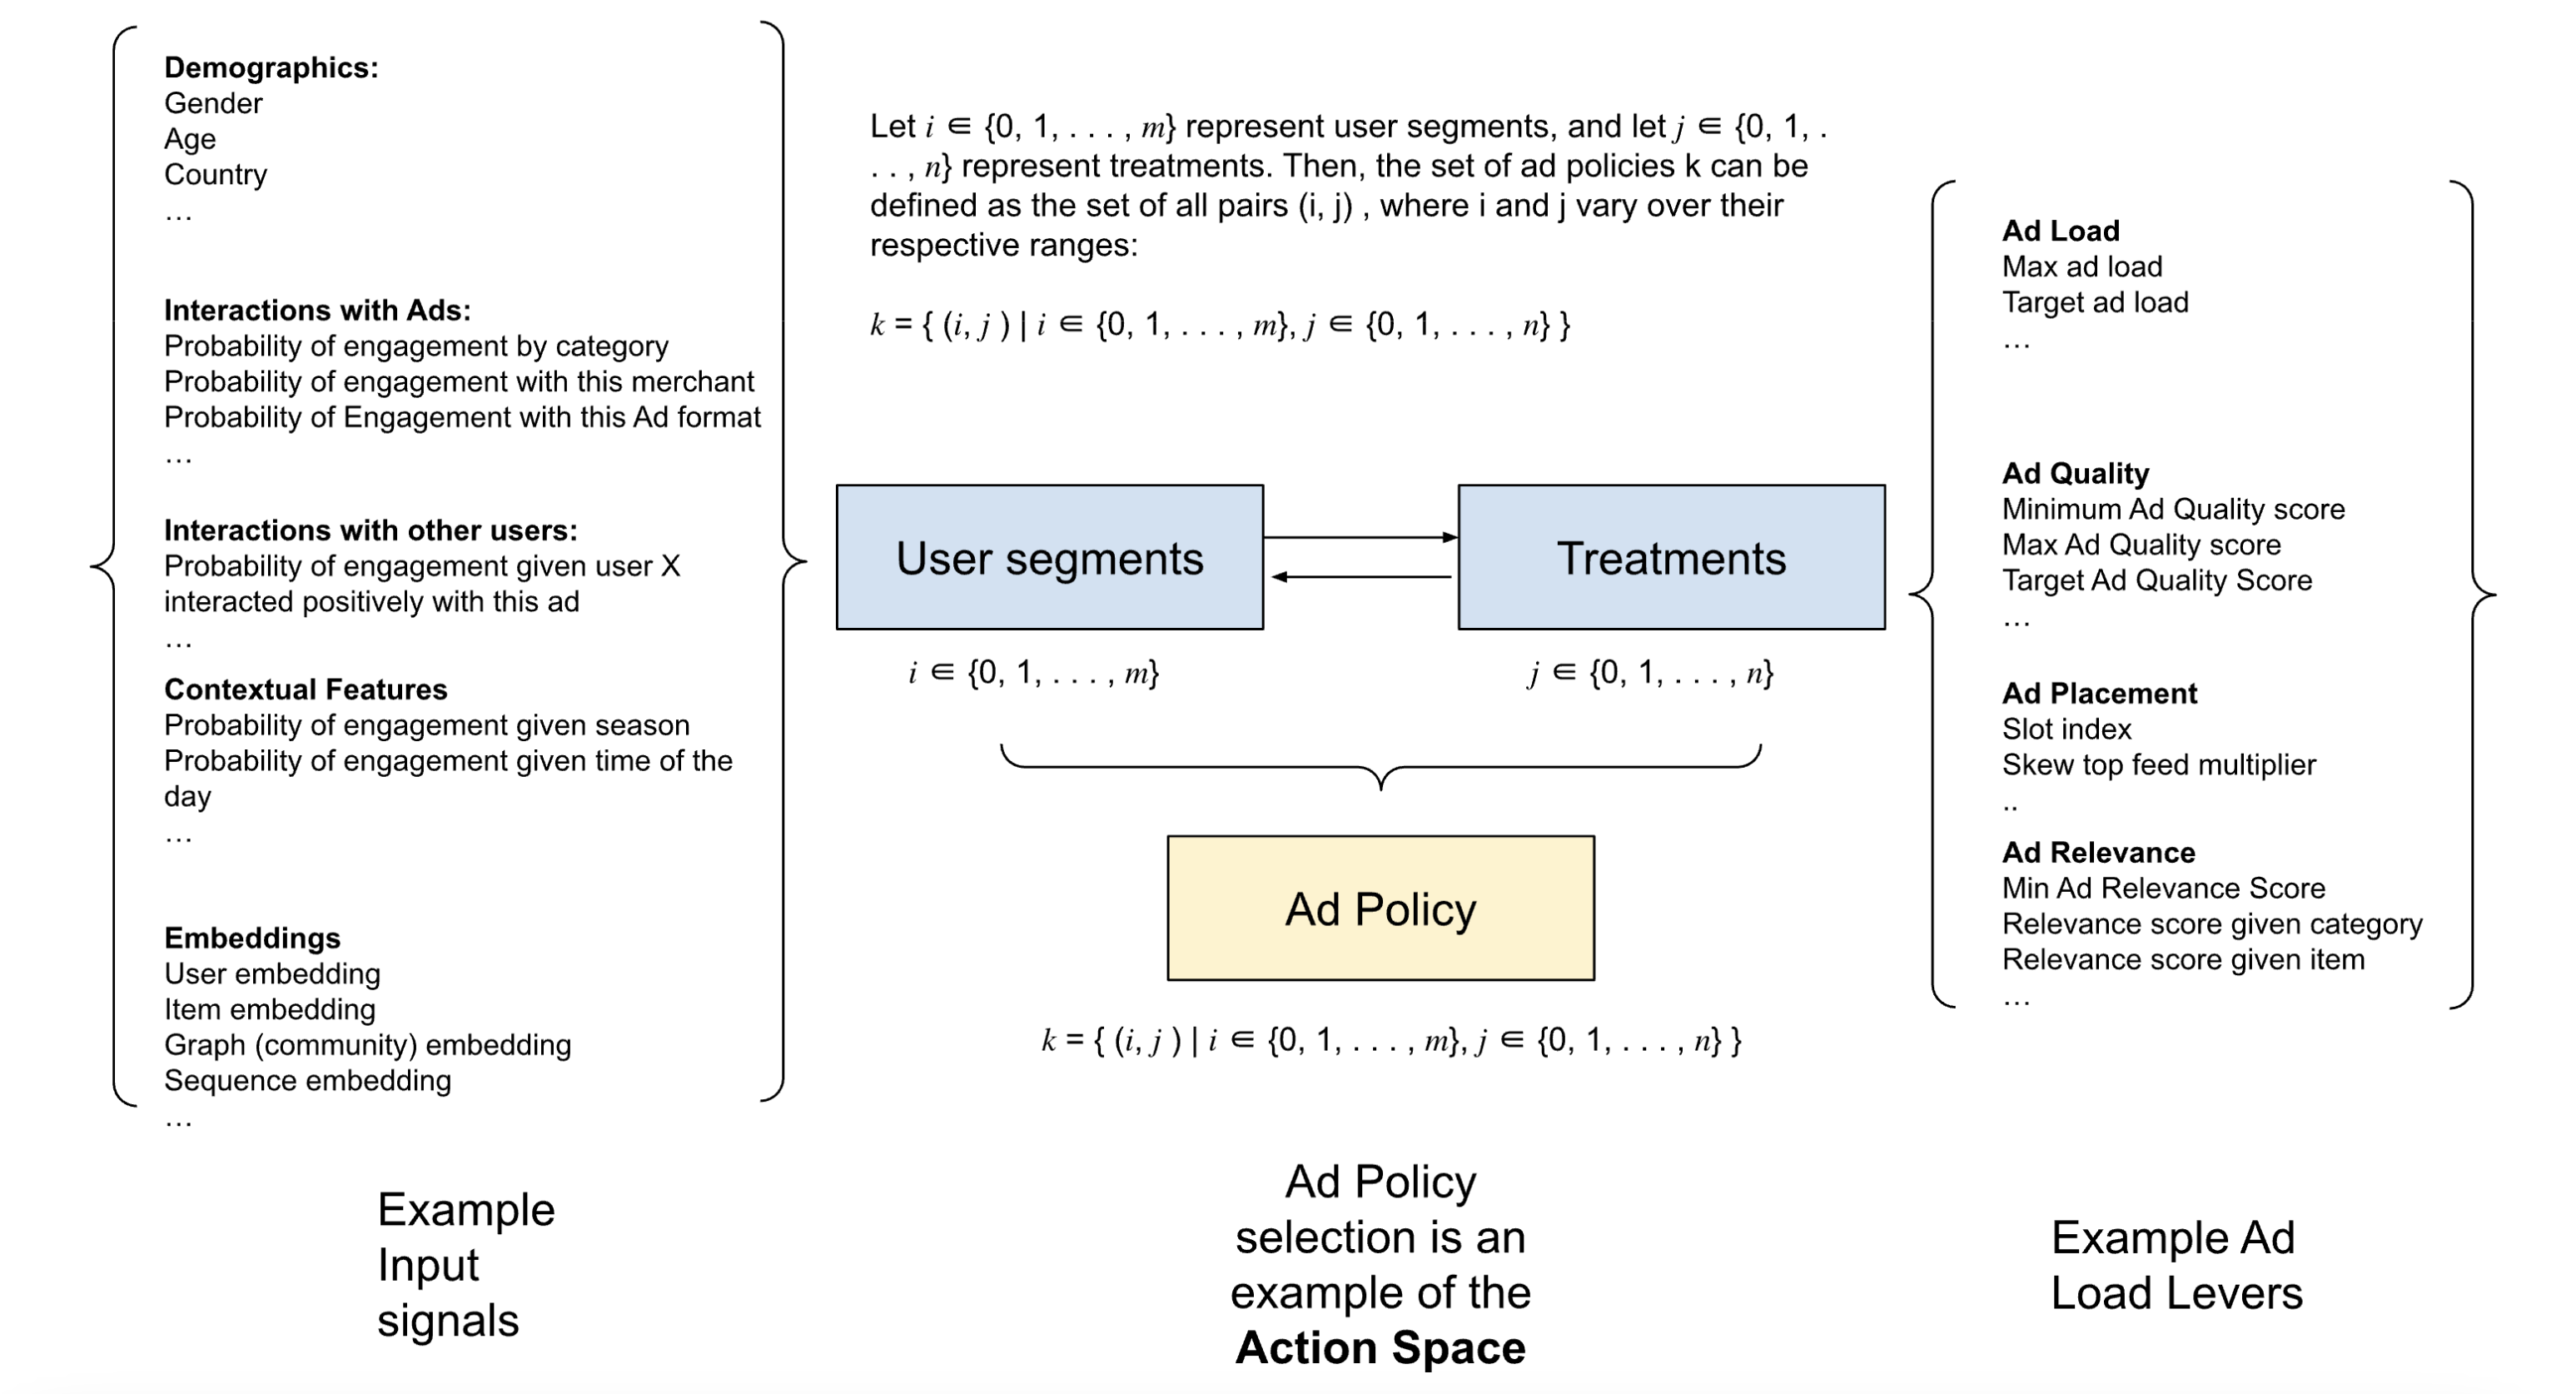
\includegraphics[width=\textwidth]{detailed_ad_policy.png}
    \caption{Example of an action set in the context of ad policies in recommendation systems}
    \label{fig:detailed_ad_policy}
\end{figure*}

\section{Conclusions}

The integration of RL in policy optimization for large-scale recommender systems has gained popularity as a promising approach to balance long-term and short-term objectives in environments with complex user behavior and revenue dynamics. However, scaling RL in practice presents challenges, including vast state and action spaces, reliance on proxy metrics, and significant computational demands. This paper provides an overview of effective, scalable techniques that address these challenges, offering insights into how RL can be applied at scale.
Unlike traditional methods that focus on optimizing short-term outcomes, RL’s cumulative reward framework enables it to account for both immediate and delayed feedback. Together, contextual bandits and offline replay offer scalable, interpretable solutions that approximate full RL while managing real-time constraints. Contextual bandits support selecting optimal actions within each interaction based on the current state, maximizing immediate rewards, which are typically proxy metrics of the true long-term reward. Offline replay complements this by enabling counterfactual learning: multiple treatments can be tested across randomized populations to evaluate causal effects, refining policies for diverse user segments.

Future research may focus on enhancing interpretability, refining reward functions, and exploring decentralized approaches to handle complex decision layers. These advancements will bring RL closer to fulfilling its potential in providing tailored, dynamic ad recommendations that align user satisfaction with business goals in large-scale recommendation systems.




\section*{Acknowledgements}
I would like to thank my advisor, Yuri Lawryshyn, for his valuable guidance and direction throughout this work. I also extend my gratitude to Adam Obeng, Bee-Chung Chen, and Jay Adams for their critical coaching and insights, which have significantly shaped my approach and understanding of industry practices. Their expertise has been key in aligning academic research with practical applications.

% This unnumbered section should be blank when submitting your paper. After review, you may include lists of people and organizations who supported the work.

% Print the biblography at the end. Keep this line after the main text of your paper, and before an appendix. 
% \input{paper.bbl}

\printbibliography
% \section{Appendix Section} \label{appdx:first}

\end{document}



\printbibliography
% \section{Appendix Section} \label{appdx:first}

\end{document}



\printbibliography
% \section{Appendix Section} \label{appdx:first}

\end{document}



% \printbibliography
\bibliography{bibliography}


% \begin{thebibliography}{99}
\bibitem{hochstein2023toward} Hochstein, Rachel E and Harmeling, Colleen M and Perko, Taylor. {T}oward a theory of consumer digital trust: meta-analytic evidence of its role in the effectiveness of user-generated content. \textit{Journal of the Academy of Marketing Science}, 1--21, 2023. Springer.

\bibitem{krizhevsky2012imagenet} Krizhevsky, Alex and Sutskever, Ilya and Hinton, Geoffrey E. {I}magenet classification with deep convolutional neural networks. \textit{Advances in neural information processing systems}, 25, 2012.

\bibitem{cui2015global} Cui, Qing and Bai, Feng-Shan and Gao, Bin and Liu, Tie-Yan. {G}lobal optimization for advertisement selection in sponsored search. \textit{Journal of Computer Science and Technology}, 30, 295--310, 2015. Springer.

\bibitem{barajas2022online} Barajas, Joel and Bhamidipati, Narayan and Shanahan, James G. {O}nline advertising incrementality testing: {P}ractical lessons, paid search and {E}merging challenges. In \textit{European Conference on Information Retrieval}, pp. 575--581. Springer, 2022.

\bibitem{kant2021history} Kant, Tanya. {A} History of the {D}ata-{T}racked {U}ser. \textit{The MIT Press Reader}, 2021. \url{https://thereader.mitpress.mit.edu/a-history-of-the-data-tracked-user/}.

\bibitem{ellam2003overture} Ellam, Andrew and Ottaviani, Marco. {O}verture and {G}oogle: {I}nternet {P}ay-{P}er-{C}lick ({P}PC) {A}dvertising {A}uctions. \textit{London Business School Case Study CS-03-022}, 2003.

\bibitem{wsj2003yahoooverture} Wall Street Journal Staff. {Y}ahoo {A}grees to {A}cquire {O}verture {F}or \textbackslash \textdollar 1.63 {B}illion. \textit{The Wall Street Journal}, 2003. \url{https://www.wsj.com/articles/SB105818965623153600}.

\bibitem{wikipedia-cpm} Wikipedia contributors. {C}ost per mille --- {W}ikipedia, {T}he {F}ree {E}ncyclopedia. [Online; accessed 23-January-2025], 2025. \url{https://en.wikipedia.org/wiki/Cost\_per\_mille}.

\bibitem{hohnhold2015focusing} Hohnhold, Henning and O\textquotesingle Brien, Deirdre and Tang, Diane. {F}ocusing on the long-term: {I}t\textquotesingle s good for users and business. In \textit{Proceedings of the 21th ACM SIGKDD International Conference on Knowledge Discovery and Data Mining}, pp. 1849--1858, 2015.

\bibitem{hu2004performance} Hu, Yu Jeffrey. {P}erformance-based pricing models in online advertising. \textit{Available at SSRN 501082}, 2004.

\bibitem{dimitrakakis2018decision} Dimitrakakis, Christos and Ortner, Ronald. {D}ecision making under uncertainty and reinforcement learning. \textit{Book available at http://www. cse. chalmers. se}, 2018. Springer.

\bibitem{koutsopoulos2016native} Koutsopoulos, Iordanis and Spentzouris, Panagiotis. {N}ative advertisement selection and allocation in social media post feeds. In \textit{Machine Learning and Knowledge Discovery in Databases: European Conference, ECML PKDD 2016, Riva del Garda, Italy, September 19-23, 2016, Proceedings, Part I 16}, pp. 588--603. Springer, 2016.

\bibitem{yan2020ads} Yan, Jinyun and Xu, Zhiyuan and Tiwana, Birjodh and Chatterjee, Shaunak. {A}ds allocation in feed via constrained optimization. In \textit{Proceedings of the 26th ACM SIGKDD International Conference on Knowledge Discovery \& Data Mining}, pp. 3386--3394, 2020.

\bibitem{russo2018tutorial} Russo, Daniel J and Van Roy, Benjamin and Kazerouni, Abbas and Osband, Ian and Wen, Zheng and others. {A} Tutorial on {T}hompson {S}ampling. \textit{Foundations and Trends\textregistered  in Machine Learning}, 11, 1--96, 2018. Now Publishers, Inc.

\bibitem{foster2020beyond} Foster, Dylan and Rakhlin, Alexander. {B}eyond ucb: {O}ptimal and efficient contextual bandits with regression oracles. In \textit{International Conference on Machine Learning}, pp. 3199--3210. PMLR, 2020.

\bibitem{fain2006sponsored} Fain, Daniel C and Pedersen, Jan O. {S}ponsored search: {A} brief history. \textit{Bulletin-American Society For Information Science And Technology}, 32, 12, 2006.

\bibitem{yi2014beyond} Yi, Xing and Hong, Liangjie and Zhong, Erheng and Liu, Nanthan Nan and Rajan, Suju. {B}eyond clicks: dwell time for personalization. In \textit{Proceedings of the 8th ACM Conference on Recommender systems}, pp. 113--120, 2014.

\bibitem{chakrabarti2008contextual} Chakrabarti, Deepayan and Agarwal, Deepak and Josifovski, Vanja. {C}ontextual advertising by combining relevance with click feedback. In \textit{Proceedings of the 17th international conference on World Wide Web}, pp. 417--426, 2008.

\bibitem{linden2003amazon} Linden, Greg and Smith, Brent and York, Jeremy. {A}mazon. com recommendations: {I}tem-to-item collaborative filtering. \textit{IEEE Internet computing}, 7, 76--80, 2003. IEEE.

\bibitem{abrams2007personalized} Abrams, Zo{\"e} and Vee, Erik. {P}ersonalized ad delivery when ads fatigue: {A}n approximation algorithm. In \textit{International Workshop on Web and Internet Economics}, pp. 535--540. Springer, 2007.

\bibitem{bietti2021contextual} Bietti, Alberto and Agarwal, Alekh and Langford, John. {A} contextual bandit bake-off. \textit{Journal of Machine Learning Research}, 22, 1--49, 2021.

\bibitem{baltescu2022itemsage} Baltescu, Paul and Chen, Haoyu and Pancha, Nikil and Zhai, Andrew and Leskovec, Jure and Rosenberg, Charles. {I}temsage: {L}earning product embeddings for shopping recommendations at pinterest. In \textit{Proceedings of the 28th ACM SIGKDD Conference on Knowledge Discovery and Data Mining}, pp. 2703--2711, 2022.

\bibitem{xia2023transact} Xia, Xue and Eksombatchai, Pong and Pancha, Nikil and Badani, Dhruvil Deven and Wang, Po-Wei and Gu, Neng and Joshi, Saurabh Vishwas and Farahpour, Nazanin and Zhang, Zhiyuan and Zhai, Andrew. {T}ransact: {T}ransformer-based realtime user action model for recommendation at pinterest. In \textit{Proceedings of the 29th ACM SIGKDD Conference on Knowledge Discovery and Data Mining}, pp. 5249--5259, 2023.

\bibitem{google_adwords_blog_2005} Google AdWords Team. {O}fficial {G}oogle {A}dWords {B}log. Accessed: 2024-12-03, 2005. \url{https://adwords.googleblog.com/2005/}.

\bibitem{pancha2022pinnerformer} Pancha, Nikil and Zhai, Andrew and Leskovec, Jure and Rosenberg, Charles. {P}innerformer: {S}equence modeling for user representation at pinterest. In \textit{Proceedings of the 28th ACM SIGKDD conference on knowledge discovery and data mining}, pp. 3702--3712, 2022.

\bibitem{he2018nais} He, Xiangnan and He, Zhankui and Song, Jingkuan and Liu, Zhenguang and Jiang, Yu-Gang and Chua, Tat-Seng. N{A}IS: {N}eural attentive item similarity model for recommendation. \textit{IEEE Transactions on Knowledge and Data Engineering}, 30, 2354--2366, 2018. IEEE.

\bibitem{Bengio1994} Bengio, Yoshua and Simard, Patrice and Frasconi, Paolo. {L}earning {L}ong-{T}erm {D}ependencies with {G}radient {D}escent is {D}ifficult. \textit{IEEE Transactions on Neural Networks}, 5, 157--166, 1994. IEEE. \url{https://www.cs.toronto.edu/\textasciitilde hinton/absps/bengio+al94.pdf}.

\bibitem{kang2018sasrec} Kang, Wang-Cheng and McAuley, Julian. {S}elf-{A}ttentive {S}equential {R}ecommendation. In \textit{Proceedings of the 2018 IEEE International Conference on Data Mining (ICDM)}, pp. 197--206, 2018. \url{https://arxiv.org/pdf/1808.09781}.

\bibitem{Sutskever2014} Sutskever, Ilya and Vinyals, Oriol and Le, Quoc V. {S}equence to sequence learning with neural networks. In \textit{Advances in Neural Information Processing Systems (NeurIPS)}, pp. 3104--3112, 2014. \url{https://papers.nips.cc/paper\_files/paper/2014/file/a14ac55a4f27472c5d894ec1c3c743d2-Paper.pdf}.

\bibitem{agarwal2020optimistic} Agarwal, Rishabh and Schuurmans, Dale and Norouzi, Mohammad. {A}n {O}ptimistic {P}erspective on {O}ffline {R}einforcement {L}earning. In \textit{International Conference on Machine Learning (ICML)}, pp. 104\textendash 114, 2020.

\bibitem{Schein2002} Schein, Andrew I. and Popescul, Alexandrin and Ungar, Lyle H. and Pennock, David M.. {M}ethods and {M}etrics for {C}old-start {R}ecommendations. In \textit{Proceedings of the 25th annual international ACM SIGIR conference on Research and development in information retrieval (SIGIR \textquotesingle 02)}, pp. 253--260, 2002.

\bibitem{Bobadilla2013} Bobadilla, Jesus and Ortega, Fernando and Hernando, Antonio and Guti\textbackslash {\'e}rrez, Arturo. {R}ecommender systems survey. \textit{Knowledge-Based Systems}, 46, 109--132, 2013.

\bibitem{Pascanu2013} Pascanu, Razvan and Mikolov, Tomas and Bengio, Yoshua. {O}n the difficulty of training recurrent neural networks. In \textit{Proceedings of the 30th International Conference on Machine Learning (ICML)}, pp. 1310--1318, 2013. PMLR. \url{http://proceedings.mlr.press/v28/pascanu13.pdf}.

\bibitem{gao2024mamba} Gao, Anningzhe and Dai, Shan and Hu, Yan. {M}amba hawkes process. \textit{arXiv preprint arXiv:2407.05302}, 2024.

\bibitem{vaswani2017attention} Vaswani, A. {A}ttention is all you need. \textit{Advances in Neural Information Processing Systems}, 2017.

\bibitem{Mehrotra2020} Rishabh Mehrotra and Niannan Xue and Mounia Lalmas. {B}andit {B}ased {O}ptimization of {M}ultiple {O}bjectives on a {M}usic 
{S}treaming {P}latform. In \textit{Proceedings of the 26th ACM SIGKDD International Conference on 
Knowledge Discovery \& Data Mining (KDD \textquotesingle 20)}, pp. 3224--3233, 2020.

\bibitem{Jannach2023} Dietmar Jannach and Himan Abdollahpouri. {A} Survey on {M}ulti-{O}bjective {R}ecommender {S}ystems. \textit{Frontiers in Big Data}, 6, 2023.

\bibitem{Mehrotra2018} Rishabh Mehrotra and James McInerney and Hugues Bouchard and  Mounia Lalmas and Fernando Diaz. {T}owards a {F}air {M}arketplace: {C}ounterfactual {E}valuation of the 
{T}rade-off between {R}elevance, {F}airness \& {S}atisfaction in 
{R}ecommendation {S}ystems. In \textit{Proceedings of the 27th ACM International Conference on Information 
and Knowledge Management (CIKM \textquotesingle 18)}, 2018.

\bibitem{Zhou2019} Guorui Zhou and Na Mou and Ying Fan and Qi Pi and Weijie Bian and  Chang Zhou and Xiaoqiang Zhu and Kun Gai. {D}eep {I}nterest {E}volution {N}etwork for {C}lick-{T}hrough {R}ate {P}rediction. In \textit{Proceedings of the 33rd AAAI Conference on Artificial Intelligence (AAAI)}, pp. 5941--5948, 2019.

\bibitem{Michel2019} Michel, Paul and Levy, Omer and Neubig, Graham. {A}re {S}ixteen {H}eads {R}eally {B}etter {T}han {O}ne?. In \textit{Advances in Neural Information Processing Systems 32 (NeurIPS)}, pp. 14014--14024, 2019.

\bibitem{Voita2019} Elena Voita and David Talbot and Fedor Moiseev and Rico Sennrich and  Ivan Titov. {A}nalyzing {M}ulti-{H}ead {S}elf-{A}ttention: {S}pecialized {H}eads {D}o the 
{H}eavy {L}ifting, the {R}est {C}an {B}e {P}runed. In \textit{Proceedings of the 57th Annual Meeting of the Association for 
Computational Linguistics (ACL)}, pp. 5797--5808, 2019.

\bibitem{Kang2018} Wang-Cheng Kang and Julian McAuley. {S}elf-{A}ttentive {S}equential {R}ecommendation. In \textit{2018 IEEE International Conference on Data Mining (ICDM)}, pp. 197--206, 2018.

\bibitem{chen2022off} Chen, Minmin and Xu, Can and Gatto, Vince and Jain, Devanshu and Kumar, Aviral and Chi, Ed. {O}ff-policy actor-critic for recommender systems. In \textit{Proceedings of the 16th ACM Conference on Recommender Systems}, pp. 338--349, 2022.

\bibitem{amodei2016concrete} Amodei, Dario and Olah, Chris and Steinhardt, Jacob and Christiano, Paul and Schulman, John and Man{\'e}, Dan. {C}oncrete problems in {A}I safety. \textit{arXiv preprint arXiv:1606.06565}, 2016.

\bibitem{carrion2021blending} Carrion, Carlos and Wang, Zenan and Nair, Harikesh and Luo, Xianghong and Lei, Yulin and Lin, Xiliang and Chen, Wenlong and Hu, Qiyu and Peng, Changping and Bao, Yongjun and others. {B}lending advertising with organic content in e-commerce: {A} virtual bids optimization approach. \textit{arXiv preprint arXiv:2105.13556}, 2021.

\bibitem{zhang2018whole} Zhang, Weiru and Wei, Chao and Meng, Xiaonan and Hu, Yi and Wang, Hao. {T}he whole-page optimization via dynamic ad allocation. In \textit{Companion Proceedings of the The Web Conference 2018}, pp. 1407--1411, 2018.

\bibitem{sagtani2024ad} Sagtani, Hitesh and Jhawar, Madan Gopal and Mehrotra, Rishabh and Jeunen, Olivier. {A}d-load {B}alancing via {O}ff-policy {L}earning in a {C}ontent {M}arketplace. In \textit{Proceedings of the 17th ACM International Conference on Web Search and Data Mining}, pp. 586--595, 2024.

\bibitem{van2016deep} Van Hasselt, Hado and Guez, Arthur and Silver, David. {D}eep reinforcement learning with double q-learning. In \textit{Proceedings of the AAAI conference on artificial intelligence}, 2016.

\bibitem{shahriari2015taking} Shahriari, Bobak and Swersky, Kevin and Wang, Ziyu and Adams, Ryan P and De Freitas, Nando. {T}aking the human out of the loop: {A} review of {B}ayesian optimization. \textit{Proceedings of the IEEE}, 104, 148--175, 2015. IEEE.

\bibitem{schulman2017proximal} Schulman, John and Wolski, Filip and Dhariwal, Prafulla and Radford, Alec and Klimov, Oleg. {P}roximal policy optimization algorithms. \textit{arXiv preprint arXiv:1707.06347}, 2017.

\bibitem{mnih2016asynchronous} Mnih, Volodymyr and Badia, Adria Puigdomenech and Mirza, Mehdi and Graves, Alex and Lillicrap, Timothy and Harley, Tim and Silver, David and Kavukcuoglu, Koray. {A}synchronous methods for deep reinforcement learning. In \textit{International conference on machine learning}, pp. 1928--1937. PMLR, 2016.

\bibitem{auer2002finite} Auer, Peter and Cesa-Bianchi, Nicolo and Fischer, Paul. {F}inite-{T}ime {A}nalysis of the {M}ultiarmed {B}andit {P}roblem. \textit{Machine learning}, 47, 235--256, 2002. Springer.

\bibitem{swaminathan2015counterfactual} Swaminathan, Adith and Joachims, Thorsten. {C}ounterfactual risk minimization: {L}earning from logged bandit feedback. In \textit{International conference on machine learning}, pp. 814--823. PMLR, 2015.

\bibitem{levine2020offline} Levine, Sergey and Kumar, Aviral and Tucker, George and Fu, Justin. {O}ffline reinforcement learning: {T}utorial, review, and perspectives on open problems. \textit{arXiv preprint arXiv:2005.01643}, 2020.

\bibitem{agarwal2014taming} Agarwal, Alekh and Hsu, Daniel and Kale, Satyen and Langford, John and Li, Lihong and Schapire, Robert. {T}aming the monster: {A} fast and simple algorithm for contextual bandits. In \textit{International conference on machine learning}, pp. 1638--1646. PMLR, 2014.

\bibitem{dudik2011doubly} Dud{\i}́k, Miroslav and Langford, John and Li, Lihong. {D}oubly robust policy evaluation and learning. \textit{arXiv preprint arXiv:1103.4601}, 2011.

\bibitem{chapelle2011empirical} Chapelle, Olivier and Li, Lihong. {A}n empirical evaluation of thompson sampling. \textit{Advances in neural information processing systems}, 24, 2011.

\bibitem{galashov2019meta} Galashov, Alexandre and Schwarz, Jonathan and Kim, Hyunjik and Garnelo, Marta and Saxton, David and Kohli, Pushmeet and Eslami, SM and Teh, Yee Whye. {M}eta-learning surrogate models for sequential decision making. \textit{arXiv preprint arXiv:1903.11907}, 2019.

\bibitem{agarwal2016statistical} Agarwal, Deepak K and Chen, Bee-Chung. {S}tatistical methods for recommender systems., 2016. Cambridge University Press.

\bibitem{chen2009large} Chen, Bee-Chung and Pavlov, Dmitry and Canny, John F and Rijckaert, Lodewijk. {L}arge-scale {B}ehavioral {T}argeting. In \textit{Proceedings of the 15th ACM SIGKDD International Conference on Knowledge Discovery \& Data Mining (KDD \textquotesingle 09)}, pp. 209--218, 2009.

\bibitem{agarwal2019online} Agarwal, Deepak and Cornell, David and Huang, Bin and Lee, Bee-Chung Chen and Tang, Ruoxi and Zhang, Le and Wolf, Avery and Shi, Yuchen and Wang, Ye and Guo, Yin and Garimella, Srijan Kumar and Korolko, Nikita and Muthukrishnan, Sandeep. {O}nline {P}arameter {S}election for {W}eb-based {S}ervices. In \textit{Proceedings of the 25th ACM SIGKDD International Conference on Knowledge Discovery \& Data Mining (KDD \textquotesingle 19)}, pp. 1645--1653, 2019.

\bibitem{sagtani2023quantifying} Sagtani, Hitesh and Jhawar, Madan Gopal and Gupta, Akshat and Mehrotra, Rishabh. {Q}uantifying and leveraging user fatigue for interventions in recommender systems. In \textit{Proceedings of the 46th International ACM SIGIR Conference on Research and Development in Information Retrieval}, pp. 2293--2297, 2023.

\bibitem{mazoure2021improving} Mazoure, Bogdan and Mineiro, Paul and Srinath, Pavithra and Sedeh, Reza Sharifi and Precup, Doina and Swaminathan, Adith. {I}mproving long-term metrics in recommendation systems using short-horizon reinforcement learning. \textit{arXiv preprint arXiv:2106.00589}, 2021.

\bibitem{everitt2021reward} Everitt, Tom and Hutter, Marcus and Kumar, Ramana and Krakovna, Victoria. {R}eward tampering problems and solutions in reinforcement learning: {A} causal influence diagram perspective. \textit{Synthese}, 198, 6435--6467, 2021. Springer.

\bibitem{zhu2021overview} Zhu, Jie and Wu, Fengge and Zhao, Junsuo. {A}n overview of the action space for deep reinforcement learning. In \textit{Proceedings of the 2021 4th International Conference on Algorithms, Computing and Artificial Intelligence}, pp. 1--10, 2021.

\bibitem{nvidia_recommender_systems_2021} Carol McDonald. {H}ow to {B}uild a {D}eep {L}earning {P}owered {R}ecommender {S}ystem, {P}art 2. Accessed: 2024-11-19, 2021. \url{https://developer.nvidia.com/blog/how-to-build-a-winning-recommendation-system-part-2-deep-learning-for-recommender-systems/}.

\bibitem{lu2016partially} Lu, Zhongqi and Yang, Qiang. {P}artially observable {M}arkov decision process for recommender systems. \textit{arXiv preprint arXiv:1608.07793}, 2016.

\bibitem{kaelbling1998planning} Kaelbling, Leslie Pack and Littman, Michael L and Cassandra, Anthony R. {P}lanning and acting in partially observable stochastic domains. \textit{Artificial intelligence}, 101, 99--134, 1998. Elsevier.

\bibitem{wu2021partially} Wu, Yaxiong and Macdonald, Craig and Ounis, Iadh. {P}artially observable reinforcement learning for dialog-based interactive recommendation. In \textit{Proceedings of the 15th ACM conference on recommender systems}, pp. 241--251, 2021.

\bibitem{silberstein2023combating} Silberstein, Natalia and Shoham, Or and Klein, Assaf. {C}ombating {A}d {F}atigue via {F}requency-{R}ecency {F}eatures in {O}nline {A}dvertising {S}ystems. In \textit{Proceedings of the 32nd ACM International Conference on Information and Knowledge Management}, pp. 4822--4828, 2023.

\bibitem{zheng2024cadrl} Zheng, Shangfei and Yin, Hongzhi and Chen, Tong and Kong, Xiangjie and Hou, Jian and Zhao, Pengpeng. C{A}DR{L}: {C}ategory-aware {D}ual-agent {R}einforcement {L}earning for {E}xplainable {R}ecommendations over {K}nowledge {G}raphs. \textit{arXiv preprint arXiv:2408.03166}, 2024.

\bibitem{chen2021user} Chen, Minmin and Chang, Bo and Xu, Can and Chi, Ed H. {U}ser response models to improve a reinforce recommender system. In \textit{Proceedings of the 14th ACM international conference on web search and data mining}, pp. 121--129, 2021.

\bibitem{wang2022surrogate} Wang, Yuyan and Sharma, Mohit and Xu, Can and Badam, Sriraj and Sun, Qian and Richardson, Lee and Chung, Lisa and Chi, Ed H and Chen, Minmin. {S}urrogate for long-term user experience in recommender systems. In \textit{Proceedings of the 28th ACM SIGKDD conference on knowledge discovery and data mining}, pp. 4100--4109, 2022.

\bibitem{zhao2021dear} Zhao, Xiangyu and Gu, Changsheng and Zhang, Haoshenglun and Yang, Xiwang and Liu, Xiaobing and Tang, Jiliang and Liu, Hui. {D}ear: {D}eep reinforcement learning for online advertising impression in recommender systems. In \textit{Proceedings of the AAAI conference on artificial intelligence}, pp. 750--758, 2021.

\bibitem{shim2022comparison} Shim, Kyuhong and Sung, Wonyong. {A} Comparison of {T}ransformer, {C}onvolutional, and {R}ecurrent {N}eural {N}etworks on {P}honeme {R}ecognition. \textit{arXiv preprint arXiv:2210.00367}, 2022. \url{https://arxiv.org/abs/2210.00367}.

\bibitem{ma2018modeling} Ma, Jiaqi and Zhao, Zhe and Yi, Xinyang and Chen, Jilin and Hong, Lichan and Chi, Ed H. {M}odeling task relationships in multi-task learning with multi-gate mixture-of-experts. In \textit{Proceedings of the 24th ACM SIGKDD international conference on knowledge discovery \& data mining}, pp. 1930--1939, 2018.

\bibitem{an2024tmh} An, Zijian and Joe, Inwhee. T{M}H: {T}wo-{T}ower {M}ulti-{H}ead {A}ttention neural network for {C}TR prediction. \textit{Plos one}, 19, e0295440, 2024. Public Library of Science San Francisco, CA USA.

\bibitem{lyu2023entire} Lyu, Shanshan and Chen, Qiwei and Zhuang, Tao and Ge, Junfeng. {E}ntire {S}pace {L}earning {F}ramework: {U}nbias {C}onversion {R}ate {P}rediction in {F}ull {S}tages of {R}ecommender {S}ystem. \textit{arXiv preprint arXiv:2303.00276}, 2023.

\bibitem{zhao2019recommending} Zhao, Zhe and Hong, Lichan and Wei, Li and Chen, Jilin and Nath, Aniruddh and Andrews, Shawn and Kumthekar, Aditee and Sathiamoorthy, Maheswaran and Yi, Xinyang and Chi, Ed. {R}ecommending what video to watch next: a multitask ranking system. In \textit{Proceedings of the 13th ACM conference on recommender systems}, pp. 43--51, 2019.

\bibitem{zou2019reinforcement} Zou, Lixin and Xia, Long and Ding, Zhuoye and Song, Jiaxing and Liu, Weidong and Yin, Dawei. {R}einforcement learning to optimize long-term user engagement in recommender systems. In \textit{Proceedings of the 25th ACM SIGKDD international conference on knowledge discovery \& data mining}, pp. 2810--2818, 2019.

\bibitem{Theocharous-2015} Theocharous, Georgios and Thomas, Philip S. and Ghavamzadeh, Mohammad. {P}ersonalized ad recommendation for life-time value optimization. In \textit{Proceedings of the 24th International Joint Conference on Artificial Intelligence (IJCAI)}, pp. 1807--1813, 2015.

\bibitem{mcdonald2023spotify} McDonald, Thomas M. and Maystre, Lucas and Lalmas, Mounia and Russo, Daniel and Ciosek, Kamil. {O}ptimizing for the {L}ong-{T}erm {W}ithout {D}elay., 2023. \url{https://research.atspotify.com/2023/07/optimizing-for-the-long-term-without-delay/}.

\bibitem{kaelbling1996reinforcement} Kaelbling, Leslie Pack and Littman, Michael L and Moore, Andrew W. {R}einforcement learning: {A} survey. \textit{Journal of artificial intelligence research}, 4, 237--285, 1996.

\bibitem{FrozenLakeGymnasium2023} . {F}rozen {L}ake {T}utorial. Accessed: 2023-03-05, 2023.

\bibitem{dulac2019challenges} Dulac-Arnold, Gabriel and Mankowitz, Daniel and Hester, Todd. {C}hallenges of real-world reinforcement learning. \textit{arXiv preprint arXiv:1904.12901}, 2019.

\bibitem{kaplan2020scaling} Kaplan, Jared and McCandlish, Sam and Henighan, Tom and Brown, Tom B and Chess, Benjamin and Child, Rewon and Gray, Scott and Radford, Alec and Wu, Jeffrey and Amodei, Dario. {S}caling laws for neural language models. \textit{arXiv preprint arXiv:2001.08361}, 2020.

\bibitem{brown2020language} Brown, Tom and Mann, Benjamin and Ryder, Nick and Subbiah, Melanie and Kaplan, Jared D and Dhariwal, Prafulla and Neelakantan, Arvind and Shyam, Pranav and Sastry, Girish and Askell, Amanda and others. {L}anguage models are few-shot learners. \textit{Advances in neural information processing systems}, 33, 1877--1901, 2020.

\bibitem{russell2016artificial} Russell, Stuart J and Norvig, Peter. {A}rtificial intelligence: a modern approach., 2016. pearson.

\bibitem{puterman2014markov} Puterman, Martin L. {M}arkov decision processes: discrete stochastic dynamic programming., 2014. John Wiley \& Sons.

\bibitem{montague1999reinforcement} Montague, P Read. {R}einforcement learning: an introduction, by {S}utton, {R}S and {B}arto, {A}G. \textit{Trends in cognitive sciences}, 3, 360, 1999. Elsevier.

\bibitem{afsar2022reinforcement} Afsar, M Mehdi and Crump, Trafford and Far, Behrouz. {R}einforcement learning based recommender systems: {A} survey. \textit{ACM Computing Surveys}, 55, 1--38, 2022. ACM New York, NY.

\bibitem{zhou2016latent} Zhou, Li and Brunskill, Emma. {L}atent contextual bandits and their application to personalized recommendations for new users. \textit{arXiv preprint arXiv:1604.06743}, 2016.

\bibitem{sharma2017learning} Sharma, Sahil and Suresh, Aravind and Ramesh, Rahul and Ravindran, Balaraman. {L}earning to factor policies and action-value functions: {F}actored action space representations for deep reinforcement learning. \textit{arXiv preprint arXiv:1705.07269}, 2017.

\bibitem{glanois2024survey} Glanois, Claire and Weng, Paul and Zimmer, Matthieu and Li, Dong and Yang, Tianpei and Hao, Jianye and Liu, Wulong. {A} survey on interpretable reinforcement learning. \textit{Machine Learning}, 1--44, 2024. Springer.

\bibitem{puiutta2020explainable} Puiutta, Erika and Veith, Eric MSP. {E}xplainable reinforcement learning: {A} survey. In \textit{International cross-domain conference for machine learning and knowledge extraction}, pp. 77--95. Springer, 2020.

\bibitem{tavakoli2018action} Tavakoli, Arash and Pardo, Fabio and Kormushev, Petar. {A}ction branching architectures for deep reinforcement learning. In \textit{Proceedings of the aaai conference on artificial intelligence}, 2018.

\bibitem{liu2025reducing} Liu, Wenzhang and Jin, Lianjun and Ren, Lu and Mu, Chaoxu and Sun, Changyin. {R}educing {A}ction {S}pace for {D}eep {R}einforcement {L}earning via {C}ausal {E}ffect {E}stimation. \textit{arXiv preprint arXiv:2501.14543}, 2025.

\bibitem{zhu2024discretizing} Zhu, Yuanyang and Wang, Zhi and Zhu, Yuanheng and Chen, Chunlin and Zhao, Dongbin. {D}iscretizing {C}ontinuous {A}ction {S}pace {W}ith {U}nimodal {P}robability {D}istributions for {O}n-{P}olicy {R}einforcement {L}earning. \textit{IEEE Transactions on Neural Networks and Learning Systems}, 2024. IEEE.

\bibitem{frozenlake} Gym Documentation Team. {F}rozen {L}ake {E}nvironment in {O}pen{A}I {G}ym. Accessed: 23 August 2024, 2024.

\bibitem{brockman2016openai} Brockman, Greg and Cheung, Vicki and Pettersson, Ludwig and Schneider, Jonas and Schulman, John and Tang, Jie and Zaremba, Wojciech. {O}pen{A}I {G}ym. \textit{arXiv preprint arXiv:1606.01540}, 2016. \url{https://arxiv.org/abs/1606.01540}.

\bibitem{danescu2010competing} Danescu-Niculescu-Mizil, Cristian and Broder, Andrei Z and Gabrilovich, Evgeniy and Josifovski, Vanja and Pang, Bo. {C}ompeting for users\textquotesingle  attention: on the interplay between organic and sponsored search results. In \textit{Proceedings of the 19th international conference on World wide web}, pp. 291--300, 2010.

\bibitem{dulac2021challenges} Dulac-Arnold, Gabriel and Levine, Nir and Mankowitz, Daniel J and Li, Jerry and Paduraru, Cosmin and Gowal, Sven and Hester, Todd. {C}hallenges of real-world reinforcement learning: definitions, benchmarks and analysis. \textit{Machine Learning}, 110, 2419--2468, 2021. Springer.

\bibitem{vonNeumannMorgenstern1944} John von Neumann and Oskar Morgenstern. {T}heory of {G}ames and {E}conomic {B}ehavior., 1944. Princeton University Press.

\bibitem{schwartz2017customer} Schwartz, Eric M and Bradlow, Eric T and Fader, Peter S. {C}ustomer acquisition via display advertising using multi-armed bandit experiments. \textit{Marketing Science}, 36, 500--522, 2017. INFORMS.

\bibitem{engel2008incorporating} Engel, Yagil and Chickering, David Maxwell. {I}ncorporating user utility into sponsored-search auctions. In \textit{Proceedings of the 7th international joint conference on Autonomous agents and multiagent systems-Volume 3}, pp. 1565--1568, 2008.

\bibitem{Stigler1950} George J. Stigler. {T}he {D}evelopment of {U}tility {T}heory. {I}. \textit{Journal of Political Economy}, 58, 307--327, 1950. University of Chicago Press.

\bibitem{wen2019learning} Wen, Ying and Mu, Yao and Ester, Martin. {L}earning {M}ulti-{O}bjective {R}ewards and {U}ser {U}tility {F}unction in {R}ecommender {S}ystems. In \textit{Proceedings of the 28th International Joint Conference on Artificial Intelligence (IJCAI)}, pp. 3719--3725. International Joint Conferences on Artificial Intelligence Organization, 2019. \url{https://www.ijcai.org/proceedings/2019/0532.pdf}.

\bibitem{kuleshov2014algorithms} Kuleshov, Volodymyr and Precup, Doina. {A}lgorithms for {M}ulti-{A}rmed {B}andit {P}roblems. \textit{arXiv preprint arXiv:1402.6028}, 2014. \url{https://arxiv.org/abs/1402.6028}.

\bibitem{thompson1933likelihood} Thompson, William R.. {O}n the likelihood that one unknown probability exceeds another in view of the evidence of two samples. \textit{Biometrika}, 25, 285--294, 1933. Oxford University Press.

\bibitem{villar2015multi} Villar, Sof{\i}́a S. and Bowden, Jack and Wason, James. {M}ulti-armed {B}andit {M}odels for the {O}ptimal {D}esign of {C}linical {T}rials: {B}enefits and {C}hallenges. \textit{Statistical Science}, 30, 199--215, 2015. Institute of Mathematical Statistics. \url{https://projecteuclid.org/euclid.ss/1432829203}.

\bibitem{burtini2015improving} Burtini, Giuseppe and Loeppky, Jason L. and Lawrence, Ramon. {I}mproving {O}nline {M}arketing {E}xperiments with {D}rifting {M}ulti-armed {B}andits. In \textit{Proceedings of the 7th International Conference on Agents and Artificial Intelligence (ICAART)}, pp. 135--146. SCITEPRESS, 2015.

\bibitem{robbins1952sequential} Herbert Robbins. {S}ome aspects of the sequential design of experiments. \textit{Bulletin of the American Mathematical Society}, 58, 527--535, 1952. \url{https://projecteuclid.org/euclid.bams/1183517370}.

\bibitem{ccelik2023ad} {\c C}elik, Fatih and {\c C}am, Mehmet Safa and Koseoglu, Mehmet Ali. {A}d avoidance in the digital context: {A} systematic literature review and research agenda. \textit{International Journal of Consumer Studies}, 47, 2071--2105, 2023. Wiley Online Library.

\bibitem{vorotilov2023scaling} Vorotilov, Vladislav and Shugaepov, Ilnur. {S}caling the {I}nstagram {E}xplore {R}ecommendations {S}ystem. \textit{Engineering at Meta}, 2023. \url{https://engineering.fb.com/2023/08/09/ml-applications/scaling-instagram-explore-recommendations-system/}.

\bibitem{zhao2024survey} Zhao, Yu and Liu, Fang. {A} survey of retrieval algorithms in ad and content recommendation systems. \textit{arXiv preprint arXiv:2407.01712}, 2024.

\bibitem{xu2023optimizing} Xu, Ruiyang and Bhandari, Jalaj and Korenkevych, Dmytro and Liu, Fan and He, Yuchen and Nikulkov, Alex and Zhu, Zheqing. {O}ptimizing long-term value for auction-based recommender systems via on-policy reinforcement learning. In \textit{Proceedings of the 17th ACM Conference on Recommender Systems}, pp. 955--962, 2023.

\bibitem{wu2018beyond} Wu, Siqi and Rizoiu, Marian-Andrei and Xie, Lexing. {B}eyond views: {M}easuring and predicting engagement in online videos. In \textit{Proceedings of the International AAAI Conference on Web and Social Media}, 2018.

\bibitem{wu2017returning} Wu, Qingyun and Wang, Hongning and Hong, Liangjie and Shi, Yue. {R}eturning is believing: {O}ptimizing long-term user engagement in recommender systems. In \textit{Proceedings of the 2017 ACM on Conference on Information and Knowledge Management}, pp. 1927--1936, 2017.

\bibitem{gauci2018horizon} Gauci, Jason and Conti, Edoardo and Liang, Yitao and Virochsiri, Kittipat and He, Yuchen and Kaden, Zachary and Narayanan, Vivek and Ye, Xiaohui and Chen, Zhengxing and Fujimoto, Scott. {H}orizon: {F}acebook\textquotesingle s open source applied reinforcement learning platform. \textit{arXiv preprint arXiv:1811.00260}, 2018.

\bibitem{yi2023progressive} Yi, Congrui and Zumwalt, David and Ni, Zijian and Chakrabarti, Shreya. {P}rogressive horizon learning: {A}daptive long term optimization for personalized recommendation. In \textit{Proceedings of the 17th ACM Conference on Recommender Systems}, pp. 940--946, 2023.

\bibitem{mcdonald2023impatient} McDonald, Thomas M and Maystre, Lucas and Lalmas, Mounia and Russo, Daniel and Ciosek, Kamil. {I}mpatient bandits: {O}ptimizing recommendations for the long-term without delay. In \textit{Proceedings of the 29th ACM SIGKDD Conference on Knowledge Discovery and Data Mining}, pp. 1687--1697, 2023.

\bibitem{lin2023survey} Lin, Yuanguo and Liu, Yong and Lin, Fan and Zou, Lixin and Wu, Pengcheng and Zeng, Wenhua and Chen, Huanhuan and Miao, Chunyan. {A} survey on reinforcement learning for recommender systems. \textit{IEEE Transactions on Neural Networks and Learning Systems}, 2023. IEEE.

\bibitem{van2024practical} van den Akker, Bram and Jeunen, Olivier and Li, Ying and London, Ben and Nazari, Zahra and Parekh, Devesh. {P}ractical {B}andits: {A}n {I}ndustry {P}erspective. In \textit{Proceedings of the 17th ACM International Conference on Web Search and Data Mining}, pp. 1132--1135, 2024.

\bibitem{li2010contextual} Li, Lihong and Chu, Wei and Langford, John and Schapire, Robert E. {A} contextual-bandit approach to personalized news article recommendation. In \textit{Proceedings of the 19th international conference on World wide web}, pp. 661--670, 2010.

\bibitem{bubeck2012regret} Bubeck, S{\'e}bastien and Cesa-Bianchi, Nicolo and others. {R}egret analysis of stochastic and nonstochastic multi-armed bandit problems. \textit{Foundations and Trends\textregistered  in Machine Learning}, 5, 1--122, 2012. Now Publishers, Inc.

\bibitem{lambert2023entangled} Lambert, Nathan and Gilbert, Thomas Krendl and Zick, Tom. {E}ntangled preferences: {T}he history and risks of reinforcement learning and human feedback. \textit{arXiv preprint arXiv:2310.13595}, 2023.

\bibitem{vouros2022explainable} Vouros, George A. {E}xplainable deep reinforcement learning: state of the art and challenges. \textit{ACM Computing Surveys}, 55, 1--39, 2022. ACM New York, NY.

\bibitem{ie2019slateq} Ie, Eugene and Jain, Vihan and Wang, Jing and Narvekar, Sanmit and Agarwal, Ritesh and Wu, Rui and Cheng, Heng-Tze and Chandra, Tushar and Boutilier, Craig. {S}late{Q}: {A} Tractable {D}ecomposition for {R}einforcement {L}earning with {R}ecommendation {S}ets.. In \textit{IJCAI}, pp. 2592--2599, 2019.

\bibitem{zhao2020jointly} Zhao, Xiangyu and Zheng, Xudong and Yang, Xiwang and Liu, Xiaobing and Tang, Jiliang. {J}ointly {L}earning to {R}ecommend and {A}dvertise. In \textit{Proceedings of the 26th ACM SIGKDD International Conference on Knowledge Discovery \& Data Mining}, pp. 3319--3327, 2020. ACM.

\bibitem{ie2019recsim} Ie, Eugene and Hsu, Chih-wei and Mladenov, Martin and Jain, Vihan and Narvekar, Sanmit and Wang, Jing and Wu, Rui and Boutilier, Craig. {R}ecsim: {A} configurable simulation platform for recommender systems. \textit{arXiv preprint arXiv:1909.04847}, 2019.

\bibitem{ie2019reinforcement} Ie, Eugene and Jain, Vihan and Wang, Jing and Narvekar, Sanmit and Agarwal, Ritesh and Wu, Rui and Cheng, Heng-Tze and Lustman, Morgane and Gatto, Vince and Covington, Paul and others. {R}einforcement learning for slate-based recommender systems: {A} tractable decomposition and practical methodology. \textit{arXiv preprint arXiv:1905.12767}, 2019.

\bibitem{mcmahan2013ad} McMahan, H Brendan and Holt, Gary and Sculley, David and Young, Michael and Ebner, Dietmar and Grady, Julian and Nie, Lan and Phillips, Todd and Davydov, Eugene and Golovin, Daniel and others. {A}d click prediction: a view from the trenches. In \textit{Proceedings of the 19th ACM SIGKDD international conference on Knowledge discovery and data mining}, pp. 1222--1230, 2013.

\bibitem{yan2009much} Yan, Jun and Liu, Ning and Wang, Gang and Zhang, Wen and Jiang, Yun and Chen, Zheng. {H}ow much can behavioral targeting help online advertising?. In \textit{Proceedings of the 18th international conference on World wide web}, pp. 261--270, 2009.

\bibitem{nielsen2017advertising} Nielsen. {W}hen {I}t {C}omes to {A}dvertising {E}ffectiveness, {W}hat {I}s {K}ey?. Accessed: 2025-03-27, 2017. \url{https://www.nielsen.com/insights/2017/when-it-comes-to-advertising-effectiveness-what-is-key/}.

\bibitem{zhao2018deep} Zhao, Jun and Qiu, Guang and Guan, Ziyu and Zhao, Wei and He, Xiaofei. {D}eep reinforcement learning for sponsored search real-time bidding. In \textit{Proceedings of the 24th ACM SIGKDD international conference on knowledge discovery \& data mining}, pp. 1021--1030, 2018.

\bibitem{saha2021advertiming} Saha, Koustuv and Liu, Yozen and Vincent, Nicholas and Chowdhury, Farhan Asif and Neves, Leonardo and Shah, Neil and Bos, Maarten W. {A}dvertiming matters: {E}xamining user ad consumption for effective ad allocations on social media. In \textit{Proceedings of the 2021 CHI Conference on Human Factors in Computing Systems}, pp. 1--18, 2021.

\bibitem{yuan2020unbiased} Yuan, Bowen and Liu, Yaxu and Hsia, Jui-Yang and Dong, Zhenhua and Lin, Chih-Jen. {U}nbiased {A}d click prediction for position-aware advertising systems. In \textit{Proceedings of the 14th ACM Conference on Recommender Systems}, pp. 368--377, 2020.

\bibitem{tettoni2024discoverability} Anne-Laure Tettoni and Simon Dumas Primbault. {D}iscoverability in a {D}igital {L}ibrary: {A} Study of \textasciigrave \textasciigrave {R}abbit {H}oles\textquotesingle \textquotesingle  within {G}allica\textquotesingle s corpus. In \textit{Proceedings of the Computational Humanities Research Conference}, pp. 1-20, 2024.

\bibitem{barré2024latent} Jean Barr{\'e}. {L}atent structures in french fiction. In \textit{Proceedings of the Computational Humanities Research Conference}, pp. 21-36, 2024.

\bibitem{arnold2024automated} Taylor Arnold and Lauren Tilton. {A}utomated {I}mage {C}olor {M}apping for a {H}istoric {P}hotographic {C}ollection. In \textit{Proceedings of the Computational Humanities Research Conference}, pp. 37-47, 2024.

\bibitem{bambaci2024steps} Luigi Bambaci and George Kiraz and Christine Roughan and Matthieu Freyder and Daniel St{\"o}kl Ben Ezra. {S}teps {T}owards {M}ining {M}anuscript {I}mages for {U}ntranscribed {T}exts: {A} Case {S}tudy {F}rom the {S}yriac {C}ollection at the {V}atican {L}ibrary. In \textit{Proceedings of the Computational Humanities Research Conference}, pp. 48-64, 2024.

\bibitem{levenson2024textual} Matthias Gille Levenson and Lucence Ing and Jean-Baptiste Camps. {T}extual {T}ransmission without {B}orders: {M}ultiple {M}ultilingual {A}lignment and {S}temmatology of the \textasciigrave \textasciigrave {L}ancelot en prose\textquotesingle \textquotesingle  ({M}edieval {F}rench, {C}astilian, {I}talian). In \textit{Proceedings of the Computational Humanities Research Conference}, pp. 65-92, 2024.

\bibitem{jacobsen2024admiration} Mia Jacobsen and Ross Deans Kristensen-McLachlan. {A}dmiration and {F}rustration: {A} Multidimensional {A}nalysis of {F}anfiction. In \textit{Proceedings of the Computational Humanities Research Conference}, pp. 93-112, 2024.

\bibitem{ströbel2024bringing} Phillip B. Str{\"o}bel and Zejie Guo and {\"U}lk{\"u} Karag{\"o}z and Eva Maria Willi and Felix K. Maier. {B}ringing {R}ome to {L}ife: {E}valuating {H}istorical {I}mage {G}eneration. In \textit{Proceedings of the Computational Humanities Research Conference}, pp. 113-126, 2024.

\bibitem{zapata2024transformation} Pepe Ballesteros Zapata and Nina Arnold and Vappu Lukander and Ludovica Schaerf and Dario Negueruela del Castillo. {T}ransformation of {C}omposition and {G}aze {I}nteraction in {N}oli {M}e {T}angere {D}epictions from 1300\textendash 1600. In \textit{Proceedings of the Computational Humanities Research Conference}, pp. 127-136, 2024.

\bibitem{moss2024modeling} Fabian C. Moss and Eita Nakamura. {M}odeling the {E}volution of {H}armony in {P}opular {M}usic from {D}ifferent {C}ultural {C}ontexts. In \textit{Proceedings of the Computational Humanities Research Conference}, pp. 137-152, 2024.

\bibitem{lassen2024literary} Ida Marie S. Lassen and Pascale Feldkamp Moreira and Yuri Bizzoni and Kristoffer Nielbo. {L}iterary {C}anonicity and {A}lgorithmic {F}airness: {T}he {E}ffect of {A}uthor {G}ender on {C}lassification {M}odels. In \textit{Proceedings of the Computational Humanities Research Conference}, pp. 153-171, 2024.

\bibitem{bizzoni2024global} Yuri Bizzoni and Pascale Feldkamp and Kristoffer Nielbo. {G}lobal {C}oherence, {L}ocal {U}ncertainty - {T}owards a {T}heoretical {F}ramework for {A}ssessing {L}iterary {Q}uality. In \textit{Proceedings of the Computational Humanities Research Conference}, pp. 172-185, 2024.

\bibitem{zhou2024once} Naitian Zhou and David Bamman. {O}nce {M}ore, {W}ith {F}eeling: {M}easuring {E}motion of {A}cting {P}erformances in {C}ontemporary {A}merican {F}ilm. In \textit{Proceedings of the Computational Humanities Research Conference}, pp. 186-199, 2024.

\bibitem{gorène2024enhancing} Chahan Vidal-Gor{\`e}ne and Cl{\'e}ment Salah and No{\"e}mie Lucas and Ali{\'e}nor Decours-Perez and Antoine Perrier. {E}nhancing {A}rabic {M}aghribi {H}andwritten {T}ext {R}ecognition with {R}AS{A}M 2: {A} Comprehensive {D}ataset and {B}enchmarking. In \textit{Proceedings of the Computational Humanities Research Conference}, pp. 200-216, 2024.

\bibitem{neugarten2024catching} Julia Neugarten and Tess Dejaeghere and Pranaydeep Singh and Amanda Robin Hemmons and Julie M. Birkholz. {C}atching {F}eelings: {A}spect-{B}ased {S}entiment {A}nalysis for {F}anfiction {C}omments about {G}reek {M}yth. In \textit{Proceedings of the Computational Humanities Research Conference}, pp. 217-231, 2024.

\bibitem{griebel2024locating} Sarah Griebel and Becca Cohen and Lucian Li and Jiayu Liu and Jaihyun Park and Jana Perkins and Ted Underwood. {L}ocating the {L}eading {E}dge of {C}ultural {C}hange. In \textit{Proceedings of the Computational Humanities Research Conference}, pp. 232-245, 2024.

\bibitem{gabay2024birth} Simon Gabay and Thibault Cl{\'e}rice. {T}he birth of {F}rench orthography. {A} computational analysis of {F}rench spelling systems in diachrony. In \textit{Proceedings of the Computational Humanities Research Conference}, pp. 246-264, 2024.

\bibitem{karsdorp2024beyond} Folgert Karsdorp and Mike Kestemont and Margo de Koster. {B}eyond the {R}egister: {D}emographic {M}odeling of {A}rrest {P}atterns in 1879-1880 {B}russels. In \textit{Proceedings of the Computational Humanities Research Conference}, pp. 265-281, 2024.

\bibitem{konle2024on} Leonard Konle and Merten Kr{\"o}ncke and Fotis Jannidis and Simone Winko. {O}n the {U}nity of {L}iterary {C}hange. {T}he {D}evelopment of {E}motions in {G}erman {P}oetry, {P}rose, and {D}rama between 1850 and 1920 as a {T}est {C}ase. In \textit{Proceedings of the Computational Humanities Research Conference}, pp. 282-300, 2024.

\bibitem{dunbar2024getting} Maria Bekker-Nielsen Dunbar and Manex Agirrezabal and T{\o}nnes Bekker-Nielsen. {G}etting to grippe with influenza: an investigation of why the disease is called that. In \textit{Proceedings of the Computational Humanities Research Conference}, pp. 301-312, 2024.

\bibitem{priestley2024treebanks} Joel Priestley and Anders N{\o}klestad and Kristin Hagen and Anu Laanemets and Dag Trygve Truslew Haug. {T}reebanks for the ordinary working grammarian. In \textit{Proceedings of the Computational Humanities Research Conference}, pp. 313-321, 2024.

\bibitem{yu2024across} Ze Yu and Federico Pianzola. {A}cross the {P}ages: {A} Comparative {S}tudy of {R}eader {R}esponse to {W}eb {N}ovels in {C}hinese and {E}nglish on {Q}idian and {W}eb{N}ovel. In \textit{Proceedings of the Computational Humanities Research Conference}, pp. 322-333, 2024.

\bibitem{rodilla2024addressing} Patricia Martin-Rodilla and Leticia Tobalina-Pulido. {A}ddressing {U}ncertainty according to the {A}nnotator\textquotesingle s {E}xpertise in {A}rchaeological {D}ata {C}ollections: an {A}pproach from {F}uzzy {L}ogic. In \textit{Proceedings of the Computational Humanities Research Conference}, pp. 334-352, 2024.

\bibitem{kaldeli2024combining} Eirini Kaldeli and Alexandros Chortaras and Vassilis Lyberatos and Jason Liartis and Spyridon Kantarelis and Giorgos Stamou. {C}ombining {A}utomatic {A}nnotation with {H}uman {V}alidation for the {S}emantic {E}nrichment of {C}ultural {H}eritage {M}etadata. In \textit{Proceedings of the Computational Humanities Research Conference}, pp. 353-368, 2024.

\bibitem{schmidt2024fine} Gleb Schmidt and Veronica Vybornaya and Ivan P. Yamshchikov. {F}ine-{T}uning {P}re-{T}rained {L}anguage {M}odels for {A}uthorship {A}ttribution of the {P}seudo-{D}ionysian {A}rs {R}hetorica. In \textit{Proceedings of the Computational Humanities Research Conference}, pp. 369-385, 2024.

\bibitem{schöch2024multilingual} Christof Sch{\"o}ch and Julia Dudar and Evgeniia Fileva and Artjoms {\v S}e{\c l}a. {M}ultilingual {S}tylometry: {T}he influence of language on the performance of authorship attribution using corpora from the {E}uropean {L}iterary {T}ext {C}ollection ({E}LTe{C}). In \textit{Proceedings of the Computational Humanities Research Conference}, pp. 386-408, 2024.

\bibitem{ros2024epistemic} Ruben Ros and Melvin Wevers. {E}pistemic {C}apture through {S}pecialization in {P}ost-{W}orld {W}ar {I}I {P}arliamentary {D}ebate. In \textit{Proceedings of the Computational Humanities Research Conference}, pp. 409-426, 2024.

\bibitem{kiessling2024does} Benjamin Kiessling and Thibault Cl{\'e}rice. {D}oes {C}ontext {M}atter ? {E}nhancing {H}andwritten {T}ext {R}ecognition with {M}etadata in {H}istorical {M}anuscripts. In \textit{Proceedings of the Computational Humanities Research Conference}, pp. 427-442, 2024.

\bibitem{hagen2024domain} Thora Hagen. {D}omain {A}daptation with {L}inked {E}ncyclopedic {D}ata: {A} Case {S}tudy for {H}istorical {G}erman. In \textit{Proceedings of the Computational Humanities Research Conference}, pp. 443-461, 2024.

\bibitem{pannach2024golem} Franziska Pannach and Luotong Cheng and Federico Pianzola. {T}he {G}OL{E}M-{K}nowledge {G}raph and {S}earch {I}nterface: {P}erspectives into {N}arrative and {F}iction. In \textit{Proceedings of the Computational Humanities Research Conference}, pp. 462-471, 2024.

\bibitem{kababgi2024recognising} Daniel Kababgi and Giulia Grisot and Federico Pennino and Berenike Herrmann. {R}ecognising non-named spatial entities in literary texts: a novel spatial entities classifier. In \textit{Proceedings of the Computational Humanities Research Conference}, pp. 472-481, 2024.

\bibitem{nagy2024bootstrap} Ben Nagy. {B}ootstrap {D}istance {I}mposters: {H}igh precision authorship verification with improved interpretability. In \textit{Proceedings of the Computational Humanities Research Conference}, pp. 482-493, 2024.

\bibitem{bamman2024on} David Bamman and Kent K. Chang and Li Lucy and Naitian Zhou. {O}n {C}lassification with {L}arge {L}anguage {M}odels in {C}ultural {A}nalytics. In \textit{Proceedings of the Computational Humanities Research Conference}, pp. 494-527, 2024.

\bibitem{mahowald2024integrating} Jamie Mahowald and Benjamin Charles Germain Lee. {I}ntegrating {V}isual and {T}extual {I}nputs for {S}earching {L}arge-{S}cale {M}ap {C}ollections with {C}LI{P}. In \textit{Proceedings of the Computational Humanities Research Conference}, pp. 528-547, 2024.

\bibitem{sartini2024deciphering} Bruno Sartini. {D}eciphering {S}till {L}ife {A}rtworks with {L}inked {O}pen {D}ata. In \textit{Proceedings of the Computational Humanities Research Conference}, pp. 548-558, 2024.

\bibitem{arnold2024explainable} Taylor Arnold and Lauren Tilton. {E}xplainable {S}earch and {D}iscovery of {V}isual {C}ultural {H}eritage {C}ollections with {M}ultimodal {L}arge {L}anguage {M}odels. In \textit{Proceedings of the Computational Humanities Research Conference}, pp. 559-574, 2024.

\bibitem{stewart2024methodology} Spencer Dean Stewart. {A} Methodology for {S}tudying {L}inguistic and {C}ultural {C}hange in {C}hina, 1900-1950. In \textit{Proceedings of the Computational Humanities Research Conference}, pp. 575-588, 2024.

\bibitem{wang2024quantitative} Sungpil Wang and Juyong Park. {Q}uantitative {F}ramework for {W}ord-{C}olor {A}ssociation and {A}pplication to 20th {C}entury {A}nglo-{A}merican {P}oetry. In \textit{Proceedings of the Computational Humanities Research Conference}, pp. 589-609, 2024.

\bibitem{raffaelli2024promises} Giulio Tani Raffaelli. {P}romises from an {I}nferential {A}pproach in {C}lassical {L}atin {A}uthorship {A}ttribution. In \textit{Proceedings of the Computational Humanities Research Conference}, pp. 610-619, 2024.

\bibitem{nusch2024clustering} Carlos Javier Nusch and Gimena Del R{\'\i}o Riande and Leticia Cagnina and Marcelo Luis Errecalde and Leandro Antonelli. {C}lustering {T}asks and {D}ecision {T}rees with {A}ugustan {L}ove {P}oets: {C}ohesion and {S}eparation in {F}eature {I}mportance {E}xtraction. In \textit{Proceedings of the Computational Humanities Research Conference}, pp. 620-648, 2024.

\bibitem{heřmánková2024fair} Petra He{\v r}m{\'a}nkov{\'a} and Brian Ballsun-Stanton and Ray Laurence. F{A}IR {T}urn in {E}pigraphy: {L}ow {B}arrier {P}athways to {Q}uantitative and {R}eproducible {R}esearch in {L}atin {E}pigraphy. In \textit{Proceedings of the Computational Humanities Research Conference}, pp. 649-661, 2024.

\bibitem{laato2024extracting} Joonatan Laato and Jenna Kanerva and John Loehr and Virpi Lummaa and Filip Ginter. {E}xtracting {S}ocial {C}onnections from {F}innish {K}arelian {R}efugee {I}nterviews {U}sing {L}LMs. In \textit{Proceedings of the Computational Humanities Research Conference}, pp. 662-680, 2024.

\bibitem{feldkamp2024sentiment} Pascale Feldkamp and Ea Overgaard Lindhardt and Kristoffer L. Nielbo and Yuri Bizzoni. {S}entiment {B}elow the {S}urface: {O}missive and {E}vocative {S}trategies in {L}iterature and {B}eyond. In \textit{Proceedings of the Computational Humanities Research Conference}, pp. 681-706, 2024.

\bibitem{barakat2024computational} Berat Kurar-Barakat and Daria Vasyutinsky-Shapira and Sharva Gogawale and Mohammad Suliman and Nachum Dershowitz. {C}omputational {P}aleography of {M}edieval {H}ebrew {S}cripts. In \textit{Proceedings of the Computational Humanities Research Conference}, pp. 707-717, 2024.

\bibitem{jacobsen2024patterns} Mia Jacobsen and Yuri Bizzoni and Pascale Feldkamp Moreira and Kristoffer L. Nielbo. {P}atterns of {Q}uality: {C}omparing {R}eader {R}eception {A}cross {F}anfiction and {C}ommercially {P}ublished {L}iterature. In \textit{Proceedings of the Computational Humanities Research Conference}, pp. 718-739, 2024.

\bibitem{boot2024in} Peter Boot and Angel Daza and Carsten Schnober and Willem van Hage. {I}n the {C}ontext of {N}arrative, we {N}ever {P}roperly {D}efined the {C}oncept of {V}alence. In \textit{Proceedings of the Computational Humanities Research Conference}, pp. 740-760, 2024.

\bibitem{ziegler2024exploration} Ismail Prada Ziegler. {E}xploration of {E}vent {E}xtraction {T}echniques in {L}ate {M}edieval and {E}arly {M}odern {A}dministrative {R}ecords. In \textit{Proceedings of the Computational Humanities Research Conference}, pp. 761-771, 2024.

\bibitem{hansen2024literary} Jens Bjerring-Hansen and Ali Al-Laith and Daniel Hershcovich and Alexander Conroy and Sebastian {\O}rtoft Rasmussen. {L}iterary {T}ime {T}ravel: {D}istinguishing {P}ast and {C}ontemporary {W}orlds in {D}anish and {N}orwegian {F}iction. In \textit{Proceedings of the Computational Humanities Research Conference}, pp. 772-787, 2024.

\bibitem{venglarova2024who} Klara Venglarova and Raven Adam and Wiltrud M{\"o}lzer and Saranya Balasubramanian and J{\"o}rn Kleinert and Manfred F{\"u}llsack and Georg Vogeler. {W}ho {A}dvertises in {N}ewspapers? {D}ata {C}riticism in {M}ining {H}istorical {J}ob {A}ds. In \textit{Proceedings of the Computational Humanities Research Conference}, pp. 788-801, 2024.

\bibitem{abel2024greatest} Edward Abel and Andrew Goddard. {G}reatest {H}its {V}ersus {D}eep {C}uts: {E}xploring {V}ariety in {S}et-lists {A}cross {A}rtists and {M}usical {G}enres. In \textit{Proceedings of the Computational Humanities Research Conference}, pp. 802-828, 2024.

\bibitem{mclachlan2024context} Ross Deans Kristensen-McLachlan and Rebecca M.M. Hicke and M{\'a}rton Kardos and Mette Thun{\o}. {C}ontext is {K}ey({N}MF): {M}odelling {T}opical {I}nformation {D}ynamics in {C}hinese {D}iaspora {M}edia. In \textit{Proceedings of the Computational Humanities Research Conference}, pp. 829-847, 2024.

\bibitem{zichert2024tracing} Michael Zichert and Adrian W{\"u}thrich. {T}racing the {D}evelopment of the {V}irtual {P}article {C}oncept {U}sing {S}emantic {C}hange {D}etection. In \textit{Proceedings of the Computational Humanities Research Conference}, pp. 848-868, 2024.

\bibitem{sobotkova2024assessing} Adela Sobotkova. {A}ssessing {B}urial {M}ound {I}ntervisibility and {P}rominence at {R}egional {S}cale. In \textit{Proceedings of the Computational Humanities Research Conference}, pp. 869-880, 2024.

\bibitem{vandyck2024abbreviation} Caroline Vandyck and Mike Kestemont. {A}bbreviation {A}pplication: {A} Stylochronometric {S}tudy of {A}bbreviations in the {O}euvre of {H}erne\textquotesingle s {S}peculum {S}cribe. In \textit{Proceedings of the Computational Humanities Research Conference}, pp. 881-891, 2024.

\bibitem{roald2024visual} Marie Roald and Magnus Breder Birkenes and Lars Gunnars{\o}nn Bag{\o}ien Johnsen. {V}isual {N}avigation of {D}igital {L}ibraries: {R}etrieval and {C}lassification of {I}mages in the {N}ational {L}ibrary of {N}orway\textquotesingle s {D}igitised {B}ook {C}ollection. In \textit{Proceedings of the Computational Humanities Research Conference}, pp. 892-905, 2024.

\bibitem{yang2024exploring} Xiaoyan Yang and Federio Pianzola. {E}xploring the {E}volution of {G}ender {P}ower {D}ifference through the {O}megaverse {T}rope on {A}O3 {F}anfiction. In \textit{Proceedings of the Computational Humanities Research Conference}, pp. 906-916, 2024.

\bibitem{chang2024subversive} Kent K. Chang and Anna Ho and David Bamman. {S}ubversive {C}haracters and {S}tereotyping {R}eaders: {C}haracterizing {Q}ueer {R}elationalities with {D}ialogue-{B}ased {R}elation {E}xtraction. In \textit{Proceedings of the Computational Humanities Research Conference}, pp. 917-937, 2024.

\bibitem{vozhik2024censorship} Ekaterina Vozhik and Kirill Maslinsky and Roman Lisiukov. {C}ensorship as a {D}issociative {F}orce: {A} Case of {S}ovremennik {M}agazine, 1847\textendash 1866. In \textit{Proceedings of the Computational Humanities Research Conference}, pp. 938-949, 2024.

\bibitem{langenhorst2024and} Jan Langenhorst and Robert C. Schuppe and Yannick Frommherz. {A}nd then {I} saw it: {T}esting {H}ypotheses on {T}urning {P}oints in a {C}orpus of {U}FO {S}ighting {R}eports. In \textit{Proceedings of the Computational Humanities Research Conference}, pp. 950-960, 2024.

\bibitem{zhang2024remember} Xinhao Zhang and Olga Seminck and Pascal Amsili. {R}emember to {F}orget: {A} Study on {V}erbatim {M}emorization of {L}iterature in {L}arge {L}anguage {M}odels. In \textit{Proceedings of the Computational Humanities Research Conference}, pp. 961-981, 2024.

\bibitem{kim2024sequencing} Alexander Kim. {S}equencing {L}iterary {R}eception: {T}rajectories of {R}ussian {N}ovels over the {A}fterlife {C}ourse. In \textit{Proceedings of the Computational Humanities Research Conference}, pp. 982-998, 2024.

\bibitem{schnober2024page} Carsten Schnober and Renate Smit and Manjusha Kuruppath and Kay Pepping and Leon van Wissen and Lodewijk Petram. {P}age {E}mbeddings: {E}xtracting and {C}lassifying {H}istorical {D}ocuments with {G}eneric {V}ector {R}epresentations. In \textit{Proceedings of the Computational Humanities Research Conference}, pp. 999-1011, 2024.

\bibitem{kurzynski2024revolution} Maciej Kurzynski and Aaron Gilkison. {R}evolution + {L}ove: {M}easuring the {E}ntanglements of {S}tate {V}iolence and {E}motions in {E}arly {P}RC. In \textit{Proceedings of the Computational Humanities Research Conference}, pp. 1012-1022, 2024.

\bibitem{häußler2024animacy} Julian H{\"a}u{\ss}ler and Janis von Keitz and Evelyn Gius. {A}nimacy in {G}erman {F}olktales. In \textit{Proceedings of the Computational Humanities Research Conference}, pp. 1023-1036, 2024.

\bibitem{bartl2024quantitative} Christoph Bartl and Sharwin Rezagholi and Mareike Schumacher. {A} quantitative study of gender representation and authors\textquotesingle  gender in a large-market print medium. In \textit{Proceedings of the Computational Humanities Research Conference}, pp. 1037-1052, 2024.

\bibitem{dalfsen2024direct} Arjan van Dalfsen and Folgert Karsdorp and Ayoub Bagheri and Dieuwertje Mentink and Thirza van Engelen and Els Stronks. {D}irect and {I}ndirect {A}nnotation with {G}enerative {A}I: {A} Case {S}tudy into {F}inding {A}nimals and {P}lants in {H}istorical {T}ext. In \textit{Proceedings of the Computational Humanities Research Conference}, pp. 1053-1074, 2024.

\bibitem{jacomy2024sub} Mathieu Jacomy and Matilde Ficozzi and Anders K. Munk. {S}ub-optimal {R}ecall in {V}isual {C}luster {R}etrieval: {W}hen {C}lusters {L}ook {L}ike {B}ridges. In \textit{Proceedings of the Computational Humanities Research Conference}, pp. 1075-1085, 2024.

\bibitem{levchenko2024automatic} Maria Levchenko. {A}utomatic {T}ranslation {A}lignment {P}ipeline for {M}ultilingual {D}igital {E}ditions of {L}iterary {W}orks. In \textit{Proceedings of the Computational Humanities Research Conference}, pp. 1086-1104, 2024.

\bibitem{hicke2024science} Rebecca M. M. Hicke and Ross Deans Kristensen-McLachlan. S{C}IE{N}CE {I}S {E}XP{L}OR{A}TI{O}N: {C}omputational {F}rontiers for {C}onceptual {M}etaphor {T}heory. In \textit{Proceedings of the Computational Humanities Research Conference}, pp. 1105-1116, 2024.

\bibitem{colliaux2024discourse} David Colliaux and Remi van Trijp. {T}he discourse of the {F}rench method: making old knowledge on market gardening accessible to machines and humans. In \textit{Proceedings of the Computational Humanities Research Conference}, pp. 1117-1127, 2024.

\bibitem{schlenk2024treating} Martin Schlenk and Thomas Efer and Manuel Burghardt. {T}reating {G}ames as {P}lays? {C}omputational {A}pproaches to the {D}etection of {S}cenes in {G}ame {D}ialogs. In \textit{Proceedings of the Computational Humanities Research Conference}, pp. 1128-1138, 2024.

\bibitem{ryan2024early} Yann Ryan and Margherita Fantoli. {E}arly {M}odern {B}ook {C}atalogues and {M}ultilingualism: {I}dentifying {M}ultilingual {T}exts and {T}ranslations using {T}itles. In \textit{Proceedings of the Computational Humanities Research Conference}, pp. 1139-1157, 2024.

\bibitem{illmer2024univariate} Viktor J. Illmer and D{\^\i}lan Canan {\c C}akir and Frank Fischer and Lilly Welz and Carsten Milling. {U}nivariate {S}tatistical {A}nalysis of a {N}on-{C}anonical {L}iterary {G}enre. {Q}uantifying {G}erman-{L}anguage {O}ne-{A}ct {P}lays (1740\textendash 1850). In \textit{Proceedings of the Computational Humanities Research Conference}, pp. 1158-1174, 2024.

\bibitem{rebora2024models} Simone Rebora and Gabriele Vezzani. {M}odels of {L}iterary {E}valuation and {W}eb 2.0. {A}n {A}nnotation {E}xperiment with {G}oodreads {R}eviews. In \textit{Proceedings of the Computational Humanities Research Conference}, pp. 1175-1200, 2024.

\bibitem{walsh2024does} Melanie Walsh and Anna Preus and Elizabeth Gronski. {D}oes {C}hat{G}PT {H}ave a {P}oetic {S}tyle?. In \textit{Proceedings of the Computational Humanities Research Conference}, pp. 1201-1219, 2024.

\bibitem{schwartz2024text} Haley Anne Schwartz and Paula Jard{\'o}n Giner and Xavier Rubio Campillo. {T}ext {M}ining to unveil {P}rehistoric {P}astness in {M}useums. In \textit{Proceedings of the Computational Humanities Research Conference}, pp. 1220-1230, 2024.

\bibitem{liew2024computational} Hong Wei Shawn Liew and Miguel Escobar Varela. {C}omputational segmentation of {W}ayang {K}ulit video recordings using a {C}ross-{A}ttention {T}emporal {M}odel. In \textit{Proceedings of the Computational Humanities Research Conference}, pp. 1231-1241, 2024.

\bibitem{maksimova2024viability} Erika Maksimova and Mari-Anna Meimer and Mari Piirsalu and Priit J{\"a}rv. {V}iability of {Z}ero-shot {C}lassification and {S}earch of {H}istorical {P}hotos. In \textit{Proceedings of the Computational Humanities Research Conference}, pp. 1242-1258, 2024.

\bibitem{kvinnsland2024rediscovering} Ranveig Kvinnsland and Ingerid L{\o}yning Dale and Lars Magne Tungland. {R}ediscovering the 1890s: {A} Norwegian {P}oetry {C}orpus. In \textit{Proceedings of the Computational Humanities Research Conference}, pp. 1259-1271, 2024.

\bibitem{wu2018budget} Wu, Di and Chen, Xiujun and Yang, Xun and Wang, Hao and Tan, Qing and Zhang, Xiaoxun and Xu, Jian and Gai, Kun. {B}udget constrained bidding by model-free reinforcement learning in display advertising. In \textit{Proceedings of the 27th ACM International Conference on Information and Knowledge Management}, pp. 1443--1451, 2018.

\bibitem{verma2018programmatically} Verma, Abhinav and Murali, Vijayaraghavan and Singh, Rishabh and Kohli, Pushmeet and Chaudhuri, Swarat. {P}rogrammatically interpretable reinforcement learning. In \textit{International conference on machine learning}, pp. 5045--5054. PMLR, 2018.

\bibitem{zhang2024scaling} Zhang, Wei and Li, Dai and Liang, Chen and Zhou, Fang and Zhang, Zhongke and Wang, Xuewei and Li, Ru and Zhou, Yi and Huang, Yaning and Liang, Dong and others. {S}caling {U}ser {M}odeling: {L}arge-scale {O}nline {U}ser {R}epresentations for {A}ds {P}ersonalization in {M}eta. In \textit{Companion Proceedings of the ACM Web Conference 2024}, pp. 47--55, 2024.

\bibitem{zhao2023embedding} Zhao, Xiangyu and Wang, Maolin and Zhao, Xinjian and Li, Jiansheng and Zhou, Shucheng and Yin, Dawei and Li, Qing and Tang, Jiliang and Guo, Ruocheng. {E}mbedding in recommender systems: {A} survey. \textit{arXiv preprint arXiv:2310.18608}, 2023.

\bibitem{koren2009matrix} Koren, Yehuda and Bell, Robert and Volinsky, Chris. {M}atrix factorization techniques for recommender systems. \textit{Computer}, 42, 30--37, 2009. IEEE.

\bibitem{quadrana2018sequence} Quadrana, Massimo and Cremonesi, Paolo and Jannach, Dietmar. {S}equence-aware recommender systems. \textit{ACM computing surveys (CSUR)}, 51, 1--36, 2018. ACM New York, NY, USA.

\bibitem{naumov2019deep} Naumov, Maxim and Mudigere, Dheevatsa and Shi, Hao-Jun Michael and Huang, Jianyu and Sundaraman, Narayanan and Park, Jongsoo and Wang, Xiaodong and Gupta, Udit and Wu, Carole-Jean and Azzolini, Alisson G and others. {D}eep learning recommendation model for personalization and recommendation systems. \textit{arXiv preprint arXiv:1906.00091}, 2019.

\bibitem{liu2022monolith} Liu, Zhuoran and Zou, Leqi and Zou, Xuan and Wang, Caihua and Zhang, Biao and Tang, Da and Zhu, Bolin and Zhu, Yijie and Wu, Peng and Wang, Ke and others. {M}onolith: real time recommendation system with collisionless embedding table. \textit{arXiv preprint arXiv:2209.07663}, 2022.

\bibitem{zhou2019deep} Zhou, Guorui and Mou, Na and Fan, Ying and Pi, Qi and Bian, Weijie and Zhou, Chang and Zhu, Xiaoqiang and Gai, Kun. {D}eep interest evolution network for click-through rate prediction. In \textit{Proceedings of the AAAI conference on artificial intelligence}, pp. 5941--5948, 2019.

\bibitem{gama2014survey} Gama, Jo{\~a}o and {\v Z}liobait{\.e}, Indr{\.e} and Bifet, Albert and Pechenizkiy, Mykola and Bouchachia, Abdelhamid. {A} survey on concept drift adaptation. \textit{ACM computing surveys (CSUR)}, 46, 1--37, 2014. ACM New York, NY, USA.

\bibitem{Zhou2018} Guorui Zhou and Chengru Song and Xiaoqiang Zhu and Ying Fan and  Han Zhu and Xiao Ma and Yanghui Yan and Junqi Jin and Han Li and Kun Gai. {D}eep {I}nterest {N}etwork for {C}lick-{T}hrough {R}ate {P}rediction. In \textit{Proceedings of the 24th ACM SIGKDD International Conference on 
Knowledge Discovery \& Data Mining (KDD \textquotesingle 18)}, pp. 1059--1068, 2018.

\bibitem{cheng2016wide} Cheng, Heng-Tze and Koc, Levent and Harmsen, Jeremiah and Shaked, Tal and Chandra, Tushar and Aradhye, Hrishi and Anderson, Glen and Corrado, Greg and Chai, Wei and Ispir, Mustafa and others. {W}ide \& deep learning for recommender systems. In \textit{Proceedings of the 1st workshop on deep learning for recommender systems}, pp. 7--10, 2016.

\bibitem{covington2016deep} Covington, Paul and Adams, Jay and Sargin, Emre. {D}eep neural networks for youtube recommendations. In \textit{Proceedings of the 10th ACM conference on recommender systems}, pp. 191--198, 2016.

\bibitem{Sutton1998} Sutton, Richard S. and Barto, Andrew G.. {R}einforcement {L}earning: {A}n {I}ntroduction., 2018 . The MIT Press. \url{http://incompleteideas.net/book/the-book-2nd.html}.

\bibitem{grbovic2018real} Grbovic, Mihajlo and Cheng, Haibin. {R}eal-time personalization using embeddings for search ranking at airbnb. In \textit{Proceedings of the 24th ACM SIGKDD international conference on knowledge discovery \& data mining}, pp. 311--320, 2018.

\bibitem{he2017neural} He, Xiangnan and Liao, Lizi and Zhang, Hanwang and Nie, Liqiang and Hu, Xia and Chua, Tat-Seng. {N}eural collaborative filtering. In \textit{Proceedings of the 26th international conference on world wide web}, pp. 173--182, 2017.

\bibitem{mikolov2013distributed} Mikolov, Tomas and Sutskever, Ilya and Chen, Kai and Corrado, Greg S and Dean, Jeff. {D}istributed representations of words and phrases and their compositionality. \textit{Advances in neural information processing systems}, 26, 2013.

\bibitem{barkan2016item2vec} Barkan, Oren and Koenigstein, Noam. {I}tem2vec: neural item embedding for collaborative filtering. In \textit{2016 IEEE 26th international workshop on machine learning for signal processing (MLSP)}, pp. 1--6. IEEE, 2016.

\bibitem{sun2019bert4rec} Sun, Fei and Liu, Jun and Wu, Jian and Pei, Changhua and Lin, Xiao and Ou, Wenwu and Jiang, Peng. B{E}RT4{R}ec: {S}equential recommendation with bidirectional encoder representations from transformer. In \textit{Proceedings of the 28th ACM international conference on information and knowledge management}, pp. 1441--1450, 2019.

\bibitem{koren2008factorization} Koren, Yehuda. {F}actorization meets the neighborhood: a multifaceted collaborative filtering model. In \textit{Proceedings of the 14th ACM SIGKDD international conference on Knowledge discovery and data mining}, pp. 426--434, 2008.

\bibitem{bennett2007netflix} Bennett, James and Lanning, Stan. {T}he netflix prize., 2007. Netflix.

\bibitem{gomez2015netflix} Gomez-Uribe, Carlos A and Hunt, Neil. {T}he netflix recommender system: {A}lgorithms, business value, and innovation. \textit{ACM Transactions on Management Information Systems (TMIS)}, 6, 1--19, 2015. ACM New York, NY, USA.

\bibitem{van2013deep} Van den Oord, Aaron and Dieleman, Sander and Schrauwen, Benjamin. {D}eep content-based music recommendation. \textit{Advances in neural information processing systems}, 26, 2013.

\bibitem{he2014practical} He, Xinran and Pan, Junfeng and Jin, Ou and Xu, Tianbing and Liu, Bo and Xu, Tao and Shi, Yanxin and Atallah, Antoine and Herbrich, Ralf and Bowers, Stuart and others. {P}ractical lessons from predicting clicks on ads at facebook. In \textit{Proceedings of the eighth international workshop on data mining for online advertising}, pp. 1--9, 2014.

\bibitem{mnih2015human} Mnih, Volodymyr and Kavukcuoglu, Koray and Silver, David and Rusu, Andrei A and Veness, Joel and Bellemare, Marc G and Graves, Alex and Riedmiller, Martin and Fidjeland, Andreas K and Ostrovski, Georg and Petersen, Stig and others. {H}uman-level control through deep reinforcement learning. \textit{Nature}, 518, 529--533, 2015. \url{https://doi.org/10.1038/nature14236}.

\bibitem{schulman2015trust} Schulman, John and Levine, Sergey and Abbeel, Pieter and Jordan, Michael and Moritz, Philipp. {T}rust region policy optimization. In \textit{International Conference on Machine Learning (ICML)}, pp. 1889--1897. PMLR, 2015. \url{https://proceedings.mlr.press/v37/schulman15.pdf}.

\bibitem{williams1992simple} Williams, Ronald J.. {S}imple statistical gradient-following algorithms for connectionist reinforcement learning. \textit{Machine Learning}, 8, 229--256, 1992. Springer. \url{https://link.springer.com/article/10.1007/BF00992696}.

\bibitem{cai2023two} Cai, Qingpeng and Xue, Zhenghai and Zhang, Chi and Xue, Wanqi and Liu, Shuchang and Zhan, Ruohan and Wang, Xueliang and Zuo, Tianyou and Xie, Wentao and Zheng, Dong and others. {T}wo-stage constrained actor-critic for short video recommendation. In \textit{Proceedings of the ACM Web Conference 2023}, pp. 865--875, 2023.
\end{thebibliography}


% \section{Appendix Section} \label{appdx:first}

\end{document}

